\chapter{Morphologische Markierungen}\label{morphologie}
 %\noindent
Im Bereich der \isi{Morphologie} weist das \hai{{\LiJi}} weit weniger Strategien zur \isi{Emulation} des Jiddischen auf, als es auf phonologischer Ebene der Fall ist. Doch selbst wenn die Quellen quantitativ nur wenige Manipulationen an der \isi{Morphologie} vornehmen, sind diese nicht minder interessant. So zeigen etwa einige der morphologischen Phänomene interessante diachrone Streuungen. In der Analyse der 53 untersuchten Quelltexte sind von der Schriftnorm abweichende Auffälligkeiten bezüglich Nominal- (Genuswahl, \isi{Diminution}, Pluralbildung, Kasussystem) und Verbalmorphologie (Flexionsformen, \isi{Wortakzent} bei Präfix-/Partikelverben) zu verzeichnen. Diese gilt es im Folgenden im Einzelnen darzulegen.

 \section{Genusverschiebungen}\label{genus}
%\noindent
 Einige Quellen des \hai{chrLiJi1} und \hai{jüdLiJi} zeigen den Gebrauch abweichender Genera. Die Genuszuweisung im Standardjiddischen entspricht (bei den Lexemen der germanischen Komponente) weitestgehend dem Deutschen (vgl.\, \citealt[166–168]{Jacobs2005}). Es gibt einige Ausnahmen, wo Variationen zwischen den drei Genera Femininum, Maskulinum und Neutrum im Standardjiddischen vorliegen, die im Deutschen nicht gegeben sind, z.\,B.\, in (\ref{BELEGEGENJI}). \,%rs + "Bsp." %LS  - Bsp.
  Es sind besonders Feminina, die zum maskulinen \isi{Genus} wechseln können. Ausnahmen wie in (\ref{bspWEIB}) \,%rs + "Bsp."%LS  - Bsp.
  lassen sich mit semantischer Kongruenz (\textit{Dehybridisierung}) erklären (vgl.\, \citealt{Fleischer2012}). Weitere Unterschiede zum deutschen Genussystem finden sich bei jüngeren Lexemen, wie z.\,B.\, in \,%rs + "Bsp."%LS  - Bsp.
  (\ref{bspHP}). Im Genussystem liegt sicherlich eine der größten Diskrepanzen zwischen Standard und gesprochener Sprache vor (\citealt[insbes. 153–207]{Wolf1969}). \label{GENUSNOJ}Dialektale Variation findet sich besonders im \hai{{\NOJ}}, wo im Unterschied zu den übrigen jiddischen Varietäten das Neutrum abgebaut und ein Genussystem entwickelt wurde, welches nur noch die Opposition \quein{maskulin–feminin} besitzt (vgl.\, \citealt{Jacobs1990b}; \citealt{Wolf1969}; \citealt[101–124]{Herzog1965}). In den Dialekten des \hai{{\NOJ}} und \hai{{\SOJ}} finden sich darüber hinaus auch Wechsel historischer Feminina zu Maskulina (\citealt[160–168]{Wolf1969}) bzw. von Maskulina zu Feminina (\citealt[168–176]{Wolf1969}). In manchen Lexemen können sogar alle drei Genera in den Dialekten auftreten, wie z.\,B.\, in \,%rs + "Bsp."%LS  - Bsp.
  (\ref{bspRAD})  (vgl.\, \citealt[178]{Wolf1969}). Eine Abweichung vom schriftdeutschen Genussystem im \hai{{\LiJi}} könnte auf diese ostjiddischen Dialektsysteme verweisen.
 
  \eenumsentence{\label{BELEGEGENJI}
\item  \RL{דער/דיע מויער} \textit{der/di moyer} \sem{die Mauer} (zitiert n.\citealt[167]{Jacobs2005})
 
\item  \RL{דער/דיע נוס} \textit{der/di nus} \sem{die Nuss}

\item  \RL{דער/דיע גרענעץ} \textit{der/di grents} \sem{die Grenze}

\item  \RL{ד{א\makebox(-1.25,-1.25)[r]{\libertineGlyph{uni05B8}}}ס/דיע וו{יי}\makebox(-1.5,-3.5)[r]{\libertineGlyph{uni207B}}ב} \textit{dos/di vayb} \sem{die Frau} (zitiert n. \citealt[167]{Jacobs2005}) \label{bspWEIB}

\item  \RL{ד{א\makebox(-1.25,-1.25)[r]{\libertineGlyph{uni05B8}}}ס/דער  וועבבלא\makebox(-1.5,-7.5)[r]{\libertineGlyph{uni207B}}ט} \textit{dos/der vebblat} \sem{die Homepage}  \label{bspHP}


\item  \RL{ד{א\makebox(-1.25,-1.25)[r]{\libertineGlyph{uni05B8}}}ס  ר{א\makebox(-1.25,-1.25)[r]{\libertineGlyph{uni05B8}}}ד} \textit{dos rod} (südl. \hai{{\ZOJ}}) – \RL{דער  ר{א\makebox(-1.25,-1.25)[r]{\libertineGlyph{uni05B8}}}ד} \textit{der rod} (\hai{{\NOJ}}) –  \RL{דיע  ר{א\makebox(-1.25,-1.25)[r]{\libertineGlyph{uni05B8}}}ד} \textit{die rod} (\hai{{\SOJ}}) \sem{das Rad}(zitiert n. \citealt[178]{Wolf1969})
 \label{bspRAD} 
  } 
 
  Diese Form der dialektalen Variation im Ostjiddischen lässt sich bis zu einem gewissen Grad auf den Einfluss, den osteuropäische Sprachen auf das Jiddische ausgeübt haben, zurückführen (vgl.\, \citealt{Trudgill1999}; \citealt[591]{Weinreich1973}). 
So sind Genus-Mismatches ein häufiges Phänomen intensiven Sprachkontakts (vgl.\, \citealt{Trudgill1999}). Dies gilt besonders in den modernen germanischen Sprachen, in denen die Genuszuweisung nicht (mehr) ersichtlich ist. Genusschwankungen und \isi{Genus}übergänge sind aber auch für die Diachronie und Diatopie des Deutschen reichlich belegt (\citealt[443f]{Schirmunski1962}). Ein Einfließen deutsch-dialektaler Formen auf das \hai{chrLiJi1} ist somit nicht völlig von der Hand zu weisen (vgl.\, \ref{BSPGENUS_6}). Möglich wäre aber auch eine rein literarische Funktion der Genusverstöße an der deutschen Schreibvarietät. So kann besonders die Verwendung des Neutrums bei Personennamen, die im Übrigen in vielen deutschen Dialekten  unmarkiert ist, in der Schriftsprache jedoch zu pejorativen Zwecken eingesetzt werden (vgl.\, \citealt{NueblingimErsch}). 
Personennamen sind im \hai{{\LiJi}} allerdings kaum von Genusverstößen betroffen. 

Die einzelnen Belege für die Setzung eines abweichenden \isi{Genus} sind in (\ref{BELEGEGENUS}) \,%rs + "Bsp." %LS - BSP.
 aufgeführt.\footnote{Alle diese Belege stehen im Nominativ, eine Kasusalternanz wäre demnach auszuschließen (vgl.\, Abschnitt \ref{kasus}).} Im \hai{chrLiJi1} finden sich einzelne Belege in sechs Quellen (\ref{BSPGENUS_1})–(\ref{BSPGENUS_7}). Das \hai{jüdLiJi1} zeigt einen einzelnen Beleg (\ref{BSPGENUS_8}). Mit Blick auf die pejorative Funktion wäre eine besondere Hervorhebung des Neutrums anzunehmen (vgl.\, \citealt{NueblingimErsch}). Dies ist jedoch nur in zwei Belegen (\ref{BSPGENUS_2} und \ref{BSPGENUS_3}) der Fall, die übrigen sechs Belege wählen das Maskulinum zur Markierung. Dies ist besonders interessant, da in vier dieser sechs Belege ein Neutrum maskulin wird, was ideal in die Strukturen des \hai{{\NOJ}} passen würde (vgl.\, \citealt{Jacobs1990}). Für einen nordostjiddischen Einfluss auf das \hai{{\LiJi}} spricht besonders die geographische Verteilung der Belege: Mit der Ausnahme einer Mannheimer Quelle liegen alle Belege im östlichen Teil des westjiddischen Sprachgebiets (vgl.\, Abbildung \ref{KarteGenus}), wo die direkte Einwanderung von Sprechern des Nordostjiddischen wahrscheinlicher ist, als im Westen bzw. Süden. 
Besonders interessant sind die Belege (\ref{BSPGENUS_1}), (\ref{BSPGENUS_5}), (\ref{BSPGENUS_7}) und (\ref{BSPGENUS_8}), \,%rs Klammern streichen, sonst auch keine, wenn direkt auf die Bsp. verwiesen wird  
 da hier das korrekte ostjiddische \isi{Genus} verwendet wird. Die Autoren müssen hier demnach eine besonders gute Kenntnis vom Ostjiddischen gehabt haben.


 \eenumsentence{\label{BELEGEGENUS}
 \item \textit{der Spektakel} \sem{das Spektakel} (\hai{BS:\,4}); vgl.\, {\oj} \RL{דער ס{פ\makebox(-1,4)[r]{\libertineGlyph{afii57807}}}עקטא\makebox(-1.5,-7.5)[r]{\libertineGlyph{uni207B}}קל} \textit{der spektakl}\label{BSPGENUS_1} %M-N %\ili{OJ}

 \item \textit{das Litteratur} \sem{die Literatur} (\hai{HJ:\,97}); vgl.\, {\oj} \RL{דיע ליטערא\makebox(-1.5,-7.5)[r]{\libertineGlyph{uni207B}}טור} \textit{di literatur}\label{BSPGENUS_2} %N-F  
 
  \item \textit{das arme Jued} \sem{der arme Jude} (\hai{WA:\,157}); vgl.\, {\oj} \RL{דער {{יי}\makebox(-1.5,-4.5)[r]{\libertineGlyph{afii57807}}}ד} \textit{der yid}\label{BSPGENUS_3}%N-M 

  \item \textit{einen guten Gehalt} \sem{ein gutes Gehalt} (\hai{FM:\,8}); \\
  vgl.\, {\oj} \RL{ד{א\makebox(-1.25,-1.25)[r]{\libertineGlyph{uni05B8}}}ס געהא\makebox(-1.5,-7.5)[r]{\libertineGlyph{uni207B}}לט} \textit{dos gehalt}\label{BSPGENUS_4}%M-N 
    
%  \item \textit{Ihrem Großtante} \sem{Ihre Großtante} (\hai{SS:\,18})\label{BSPGENUS_4.2}
 
  \item \textit{der Schiff} \sem{das Schiff} (\hai{SS:\,18}); vgl.\, {\oj} \RL{דיע שיף} \textit{die shif}\label{BSPGENUS_5} 
  %M-N %\ili{OJ}
 
  \item \textit{ein Lerche} \sem{eine Lerche} (\hai{LR:\,11});\\ 
  vgl.\, Mitteldt. (südmos. Obh.) \textit{der lerx} (\citealt[444]{Schirmunski1962}); \\
  {\oj} \RL{ד{א\makebox(-1.25,-1.25)[r]{\libertineGlyph{uni05B8}}}ס טרילערל} \textit{dos trillerl} \sem{die Lerche} \label{BSPGENUS_6}
%M-F 

  \item \textit{ein Wachtel} \sem{eine Wachtel} (\hai{LR:\,11}); \\
vgl.\, {\oj} \RL{דער ווא\makebox(-1.5,-7.5)[r]{\libertineGlyph{uni207B}}כטל} \textit{der wachtel}\label{BSPGENUS_7} %M-F %\ili{OJ}
  
  
   \item \textit{der großer Seminar} \sem{das große Seminar} (\hai{GuS23:\,4})\\
   vgl.\, {\oj} \RL{דער סעמינא\makebox(-1.5,-7.5)[r]{\libertineGlyph{uni207B}}ר} \textit{der seminar}\label{BSPGENUS_8} %jüdLIJI1 %M-N %\ili{OJ}

   
  } 




\begin{figure} 

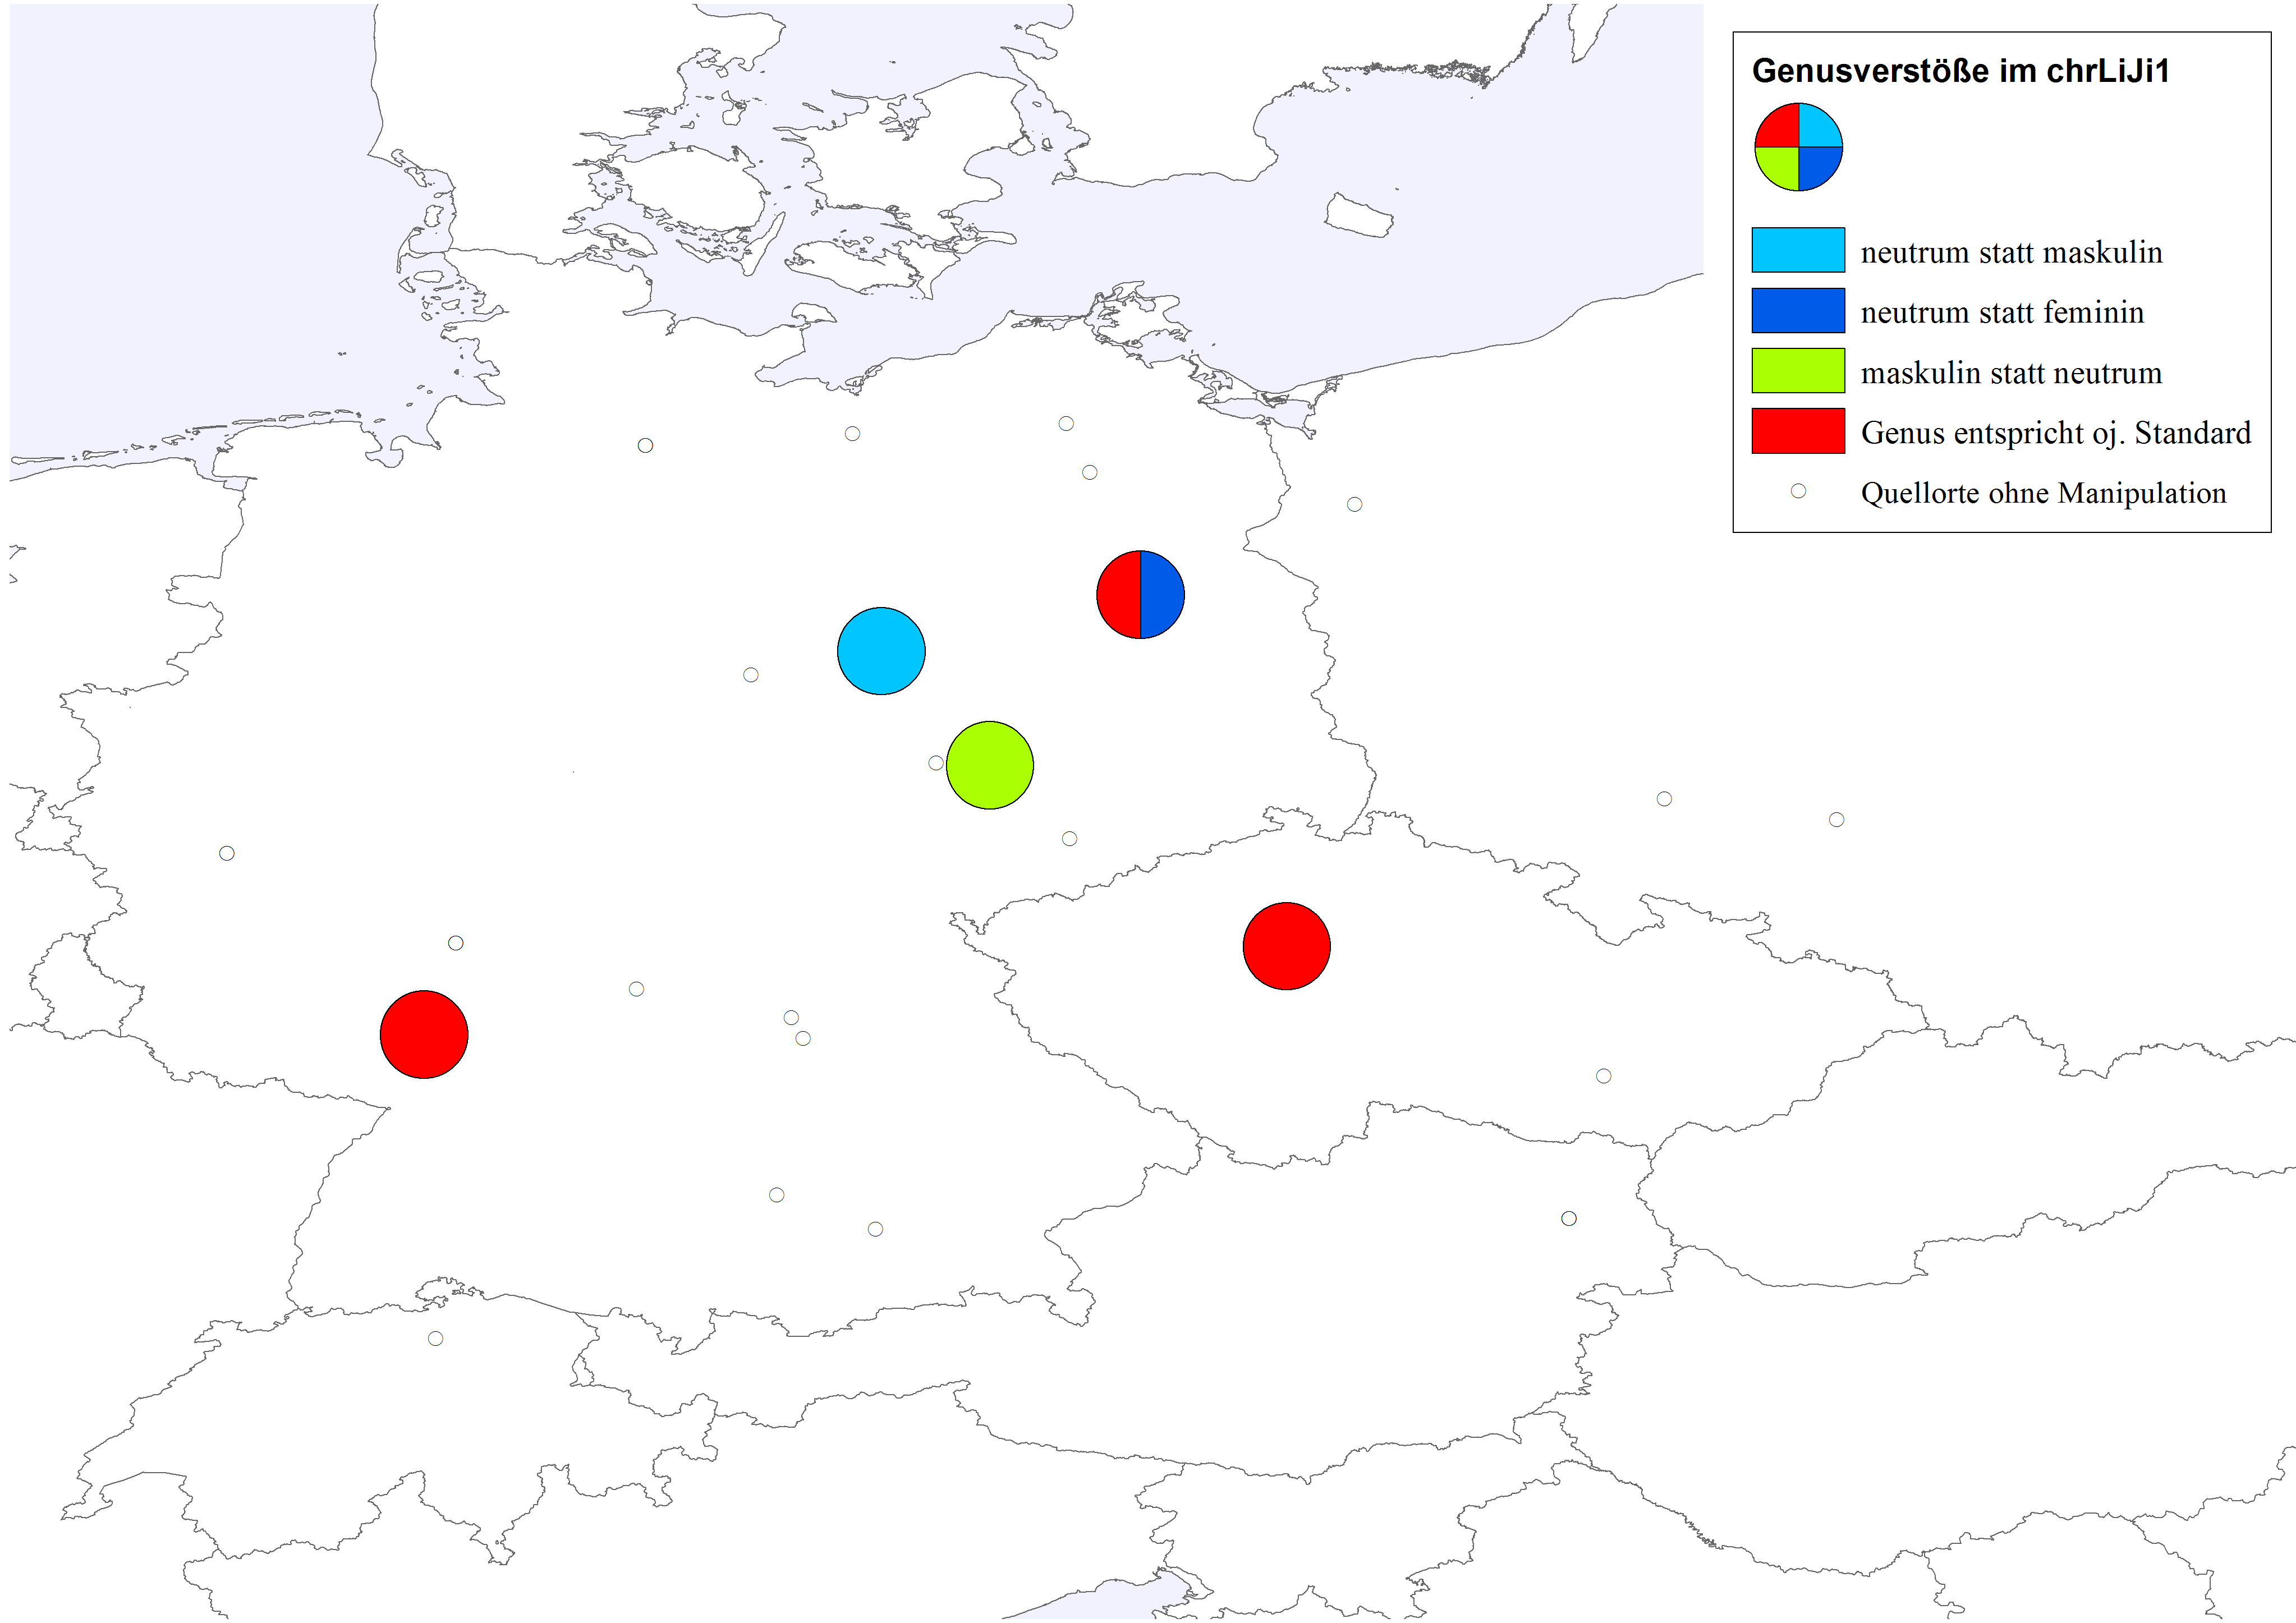
\includegraphics[width=\textwidth]{figures/KarteGenus.png}
		\caption{\label{KarteGenus} Genusverschiebungen im \hai{chrLiJi1}}
	\end{figure}
 
	 

Abschließend lässt sich festhalten, dass Genusverschiebungen von der deutschen Schriftsprache im \hai{{\LiJieins}} äußerst selten vorkommen. Die Hälfte der Belege verwenden Genera, die ostjiddischen Formen entsprechen. Dies ist erstaunlich und kann für eine Kenntnis dieser Autoren vom Ostjiddischen sprechen oder als Hinweis für ein vom Schriftdeutschen abweichendes Genussystem im Westjiddischen interpretiert werden. Wie nun die übrigen vier Belege zu interpretieren sind, muss offen bleiben. Zum einen ist es durchaus möglich, dass die entsprechenden Lexeme in den entsprechenden jiddischen Dialekten genau die Genera aufweisen, die im \hai{{\LiJieins}} belegt sind. Andererseits ist auch die pejorative Funktion von Genusverstößen nicht völlig von der Hand zu weisen. 
Plausibel erscheint es, eine Kombination zwischen Pejoration und Sprachrealität anzunehmen.


  \section{Diminutionen}\label{dim}
 %\noindent
Die \isi{Diminution} ist ein äußerst frequentes Mittel der Charakterisierung jüdischer Figuren. Es finden sich im \hai{chrLiJi1} in 39 (von 53) Quellen 12 verschiedene Diminutivsuffixe für die Singulardiminution (Tabelle \ref{tblDIMSG}, S.\, \pageref{tblDIMSG}) und in 27 Texten 14 Suffixe für die \isi{Diminution} im Plural (Tabelle \ref{tblDIMPL}, S.\, \pageref{tblDIMPL}). In vielen Texten werden dabei mehrere Suffixe parallel verwendet. Im Singular zeigen 14 Quellen zwei unterschiedliche Suffixe parallel. Insgesamt sieben Quellen verwenden drei und in jeweils einer Quelle treten vier (\hai{PA} Frankfurt, 1834) und sechs (\hai{GW} n.a., ca.\, 1900) unterschiedliche Suffixe nebeneinander auf. Der Mittelwert liegt bei 1,4 Suffixen pro Quelle (bei einer Standardabweichung von {$\sigma$}\,1,2). Sechs Quellen verwenden zwei unterschiedliche Suffixe zur Pluraldiminution; fünf Quellen drei und eine Quelle (\hai{PG} Speyer, 1835) vier Suffixe. Dies allein zeigt, welche Vielzahl an Suffixen eingesetzt wird.\label{AnzahlDIM}

Die im Jiddischen verwendeten Diminutivsuffixe entstammen der germanischen Komponente. Aus diesem Grund wird, bevor auf die \isi{Diminution} im Jiddischen eingegangen wird (Unterabschnitt \ref{dimJIDDISCH}), das deutsche System dargestellt (Unterabschnitt \ref{dimDEUTSCH}). Da das Jiddische die Unterscheidung zwischen Diminutivsingular und -plural trifft (\citealt[162–166]{Jacobs2005}), erfolgt die anschließende Analyse aufgrundlage dieser Trennung. Es werden zunächst die einzelnen im \hai{{\LiJi}}  auffindbaren Singulardiminutiva  und später die Pluraldiminutiva dargestellt und mit der Situation im Jiddischen und den deutschen Dialekten verglichen. In die Analyse nicht aufgenommen wird die semantische Kategorie des Diminutivs 1. und 2. Grades, der eine Unterscheidung zwischen \sem{verkleinernd} und \sem{verzärtlichend} trifft und für das Jiddische angenommen wird (\citealt[48]{Landau1895}; \citealt[80]{Perlmutter1988}; \citealt[162]{Jacobs2005}),\footnote{Eine solche semantische Differenzierung ist auch aus den deutschen Dialekten bekannt, wie z.\,B.\, dem Schwäbischen oder dem Hochalemannischen (vgl.\, \citealt[1250]{Seebold1983}; \citealt[159–208]{Luessy1974}; \citealt[162]{Schirmunski1962}).} da solche Kategorien bestenfalls durch direkte Sprecherbefragung, aber nur schwer aufgrundlage schriftlicher Quellen ermittelt werden können.





\subsection{Diminution in den deutschen Dialekten}\label{dimDEUTSCH}
%  %\noindent
Im Deutschen wie auch im Jiddischen erfolgt die \isi{Diminution} mittels Umlautung des Stammvokals und Suffigierung am Stamm. Für die Dialekte des Deutschen veranschlagt man abhängig vom Konsonanten des Suffixes eine grobe Einteilung in \hai{L}- und \hai{K}-\isi{Diminution} (u.\,a.\, \citealt{Wrede1908}; \citealt[475–487]{Schirmunski1962}; \citealt{Seebold1983}), d.\,h. es liegen zwei Klassen von Diminutivsuffixen vor, die sich in ihrem Basiskonsonanten unterscheiden. Dabei finden sich Diminutivformen mit -\textit{l}- als Basiskonsonant im Süden des Sprachgebiets, Formen auf -\textit{k}-(> -\textit{ch}-) im Norden (vgl.\, Abbildung \ref{tblDIMsystemSg}, S.\, \pageref{tblDIMsystemSg} u. \ref{DimDSA}, S.\, \pageref{DimDSA}).\footnote{In den dt. Dialekten der Schweiz und Österreichs, die nicht von den Wenkerkarten abgedeckt sind, setzt sich das \isi{Dialektkontinuum} fort und wir finden hier konsequent \hai{L}-\isi{Diminution}.} Diese Nord-Süd-Teilung der Dialekte spiegelt sich selbst im Schriftdeutschen wieder, wo zwei Diminutivsuffixe -\textit{chen} und -\textit{lein} gebräuchlich sind.\footnote{Mittlerweile hat sich überwiegend die ursprünglich ostmitteldeutsche Diminutivbildung mittels -\textit{chen} durchgesetzt (\citealt[475, 479]{Schirmunski1962}; \citealt[157]{Koenig1978}). Sobald der Stamm auf -\textit{ch}, -\textit{g}, oder -\textit{ng} auslautet, findet sich in der nhd. Schriftsprache die ursprünglich oberdeutsche Bildung mit -\textit{lein} (\citealt[475]{Schirmunski1962}).} Die deutschen Mundarten weisen hingegen weitaus mehr und \qu{seit langem konkurrierende Typen von Diminutivformen} auf, als die Standardsprache vermuten lässt (\citealt[476]{Schirmunski1962}). Wie \cite{Wrede1908} in seiner umfassenden Beschreibung der im Wenkermaterial erhobenen Diminutiva zeigt, ist das Auftreten eines Diminutivsuffixes in den meisten Dialekten abhängig von der \isi{Semantik} eines Lexems und dessen phonologischen Bedingungen. Tatsächlich verwenden die meisten Sprecher eines deutschen Dialekts mehr als nur ein Suffix. Die Leitformenkartierung des \hai{WA} ist damit bei diesem Phänomen stark an das einzelne Lexem gebunden (\citealt[74f]{Wrede1908}).\label{wredeDIM} Das heißt auch, dass alle nachfolgenden Kartenbilder, insbesondere die Polygone des \hai{WA}, wie auch im Fall der phonologischen Karten, nur die Variationen eines Lexems darstellen und keine Gesetzmäßigkeiten reflektieren (vgl.\, \citealt[79]{Wrede1908}). 
   
   
  Die zwei Basistypen von \isi{Diminution} bewirken je nach Vokal kleinräumige areale Variation.\, Hinzu kommen Fusionsformen beider Basistypen, wie man sie im mitteldeutschen Raum, also in der Kontaktzone zwischen \hai{L}-\, und \hai{K}-{Di\-mi\-nu\-tion}, findet. Eine Zusammenfassung der belegten Kombinationen findet sich in Tabelle \ref{tblDIMsystemSg} (S.\, \pageref{tblDIMsystemSg}) für die Singulardiminution und in Tabelle \ref{tblDIMsystem} (S.\, \pageref{tblDIMsystem}) für die Pluralformen.  
 
	Eine Trennung zwischen Singular- und Pluraldiminution, wie sie das Jiddische zeigt und welche nach den Regeln der morphologischen Natürlichkeit besondere \textit{Ikonizität} abbildet (vgl.\, \citealt[insbes. 98–102]{Mayerthaler1981}; \citealt[insbes. 59]{Wurzel1984}), kennen nur wenige deutsche Dialekte. Ausgehend von der in Tabelle \ref{tblDIMsystem} (S.\, \pageref{tblDIMsystem}) aufgeführten Typisierung werden in Abbildung \ref{DimDSA}  die Einzelformen (\hai{WA}-Karte Nr. 381) zur Pluraldiminution zu entsprechenden Polygonen zusammengefasst, die die einzelnen Typen und ihre räumliche Verbreitung darstellen.\footnote{Das Suffix \textit{-chen} verhält sich in der Typisierung als Pluraldiminutivsuffix problematisch, da es zum einen dem Typ einfacher \hai{K}-\isi{Diminution} zugerechnet werden kann; gesetzt den Fall es bestünde aus dem Diminutivsuffix \textit{-chen-} zuzüglich einem  \textit{-en}-Plural ist es zum anderen aber auch dem Typ \hai{K}+\hai{{\Pl}} zuzurechnen. Der Vergleich der Karten zum Singular- und \isi{Pluralsuffix} im \hai{WA} (Karten 381 u. 440) zeigt, dass im ostmitteldeutschen (insbes. dem Obersächsischen) \textit{-chen} sowohl als übliches Suffix zur Singular- als auch zur Pluraldiminution vorliegt. Damit ist keine Unterscheidung zwischen Singular und Plural bei der \isi{Diminution} erkennbar und das Suffix muss hier  zum einfachen \hai{K}-Typ gerechnet werden. Anders sieht es jedoch im Rheinfränkischen (insbes. zwischen Aschaffenburg u.  Weinheim) aus. Hier finden sich im Singular die Suffixe \textit{-che}, \textit{-elche}, \textit{-el} und \textit{-la}. Wir haben es also mit einer äußerst vielfältigen Region von Diminutivsuffixen im Singular zu tun. Im Plural aber findet sich hier flächendeckend \textit{-chen}. Damit unterscheidet sich das Suffix eindeutig vom Singular und die Analyse des Suffix als \hai{K}-\isi{Diminution} + \hai{{\Pl}}-Suffix erscheint hier sinnvoll, zumindest gilt dies für die Gebiete, in denen \textit{-che} und \textit{-elche} im Singular vorliegen. Aus diesem Grund wurde das entsprechende Gebiet im Rheinfränkischen in Karte \ref{DimDSA} zum \hai{K}+\hai{{\Pl}}-Gebiet gezählt, während das Gebiet im Obersächsischen, welches \textit{-chen} im Singular und im Plural aufweist, als zur reinen \hai{K}-\isi{Diminution} gehörig kartiert wurde.} Augenscheinlich ist die aus der Singulardiminution bekannte Nord-Süd-Teilung in \hai{K}- und \hai{L}-\isi{Diminution} (vgl.\, Abbildung \ref{SgDimDSA}). Ebenfalls fällt auf, dass eine besondere Pluralmarkierung vor allem in Regionen von \hai{K}-Singulardiminution und besonders im (west-)mitteldeutschen Gebiet verwendet wird. Im Süden hingegen, wo die \hai{L}-\isi{Diminution} verbreitet ist, wird kaum zwischen Plural und Singular am Diminutivum unterschieden. Die Kombination von \hai{L}-\isi{Diminution} im Singular und \hai{K + {\Pl}}-\isi{Diminution} im Plural, wie sie im Jiddischen vorliegt, ist eine seltene Ausnahme im deutschen Dialektverbund. Lediglich in den Randgebieten des Rhein- und Ostfränkischen kann man  die auf \hai{L}-\isi{Diminution} aufbauenden Pluraldiminutivsuffixe finden und hierbei unter anderem auch das aus dem Jiddischen bekannte Suffix \textit{-lich}. Dieses Suffix findet sich entlang der Isoglosse von \hai{L}- und \hai{K}-Diminutionstypen. Es ist v.\,a.\, diese geolinguistische Verortung, die dafür spricht, in dem Suffix eine Fusion der beiden Basistypen von \isi{Diminution} zu sehen, wie sie auch bei anderen Suffixen entlang der \hai{L}/\hai{K}-Isoglosse zu finden ist.\footnote{So wird der Fusionscharakter von Diminutivsuffixen im Mitteldeutschen deutlicher am Beispiel des Suffixes \textit{-elcher}, welches als eine Fusion aus \textit{-el}\textsubscript{\hai{L}-{\Dim}} + \textit{-ch(e)}\textsubscript{\hai{K}-{\Dim}} + \textit{-(e)r}\textsubscript{{\Pl}} zu analysieren ist.} \\
	
	
	
	 
  
  \begin{table}
%\begin{longtable}{cccccc}

		\begin{tabular}{ll}

		\lsptoprule 

\textbf{Muster} &\textbf{Beispiel} (\sem{Ente\textsubscript{{\Dim} {\Sg}}})  \\ \midrule 

\hai{K} & \textit{-che} \textit{Entche}, \textit{-ke} \textit{Entke} \\
\hai{L} & \textit{-le} \textit{Entla}, \textit{-ile} \textit{Entile} \\

\hai{L + K }& \textit{-elche} \textit{Entelche} \\
  \lspbottomrule 
 \end{tabular}
		 \caption{Grundmuster von Singulardiminutivsuffixen im Deutschen (basierend auf \hai{WA} Karte Nr. 440 \sem{Stückchen})}
		 \label{tblDIMsystemSg}
		 \end{table}
		% \end{longtable}
 

	
	  \begin{figure} 

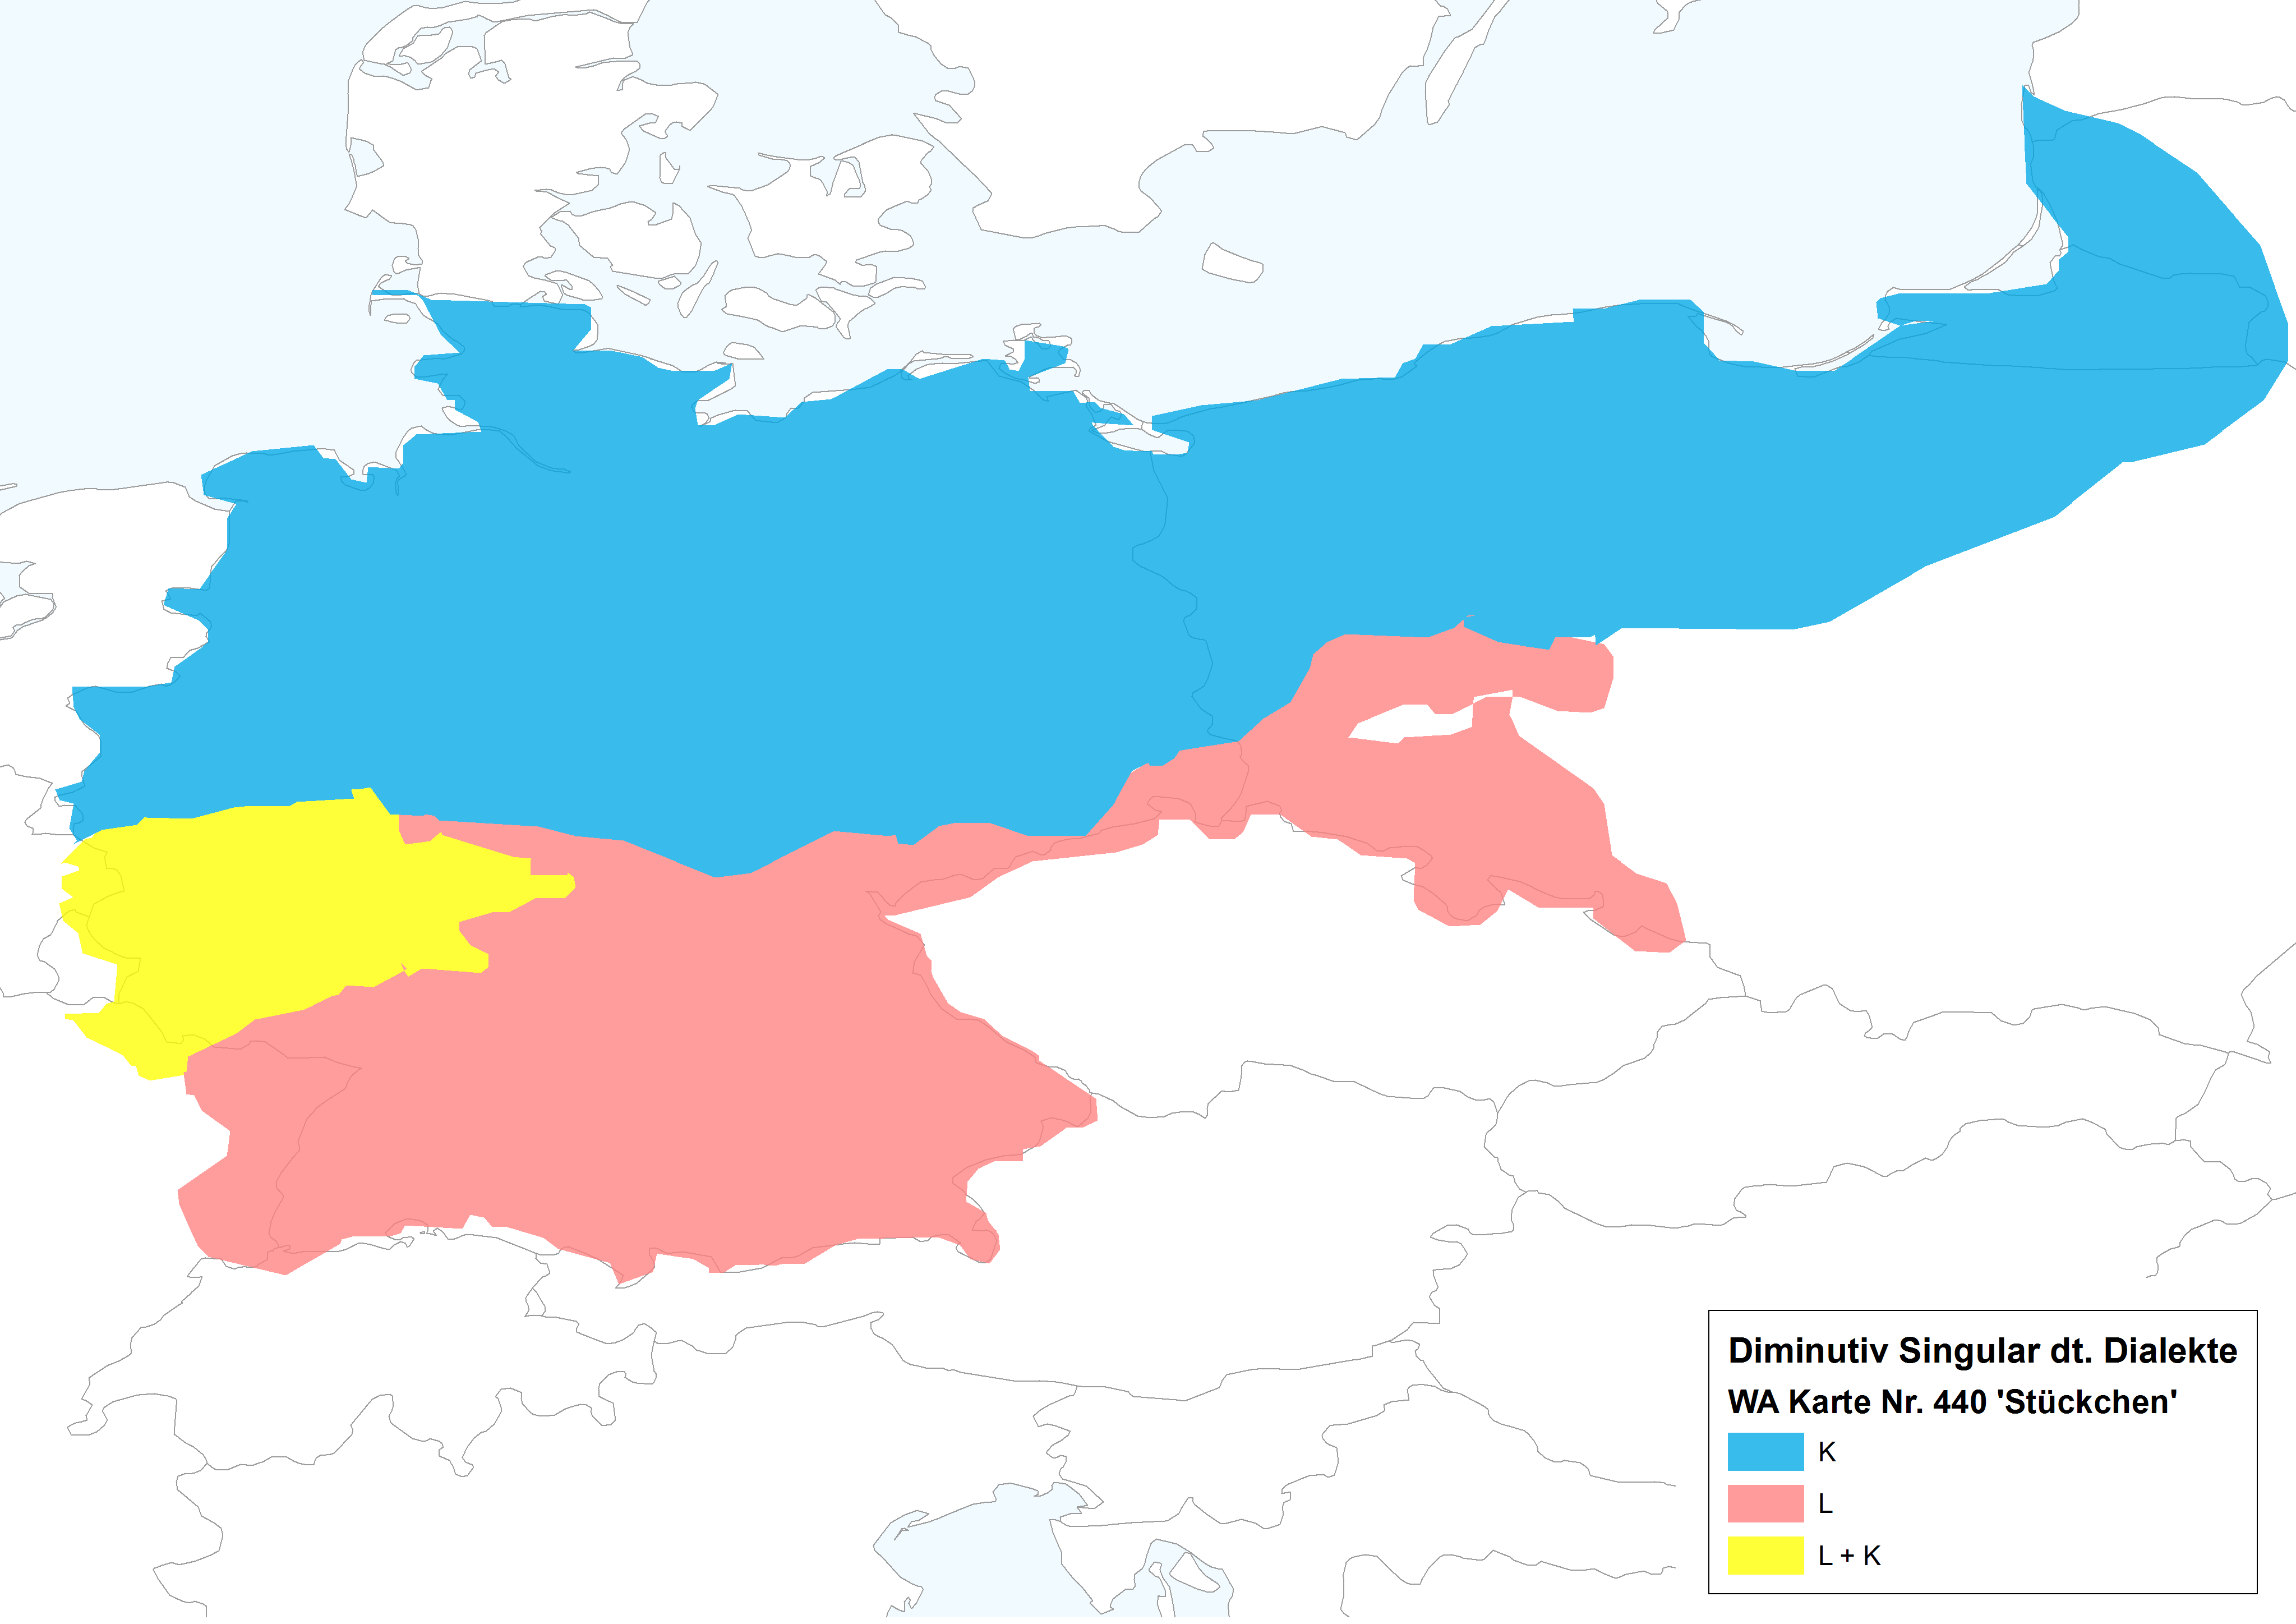
\includegraphics[width=\textwidth]{figures/DSA_DIM_SG_kurz.png}
		\caption{\label{SgDimDSA} Singulardiminutionen in den dt. Dialekten (\hai{WA} Karte Nr. 440 \sem{Stückchen})}
		\end{figure}
 


	
		
		
		
  \begin{table}
%\begin{longtable}{cccccc}

		\begin{tabular}{ll}

		\lsptoprule 

\textbf{Muster} &\textbf{Beispiel} (\sem{Ente\textsubscript{{\Dim} {\Pl}}})  \\ \midrule 

\hai{K} & \textit{-che} \textit{Entche}, \textit{-ke} \textit{Entke} \\
\hai{L} & \textit{-le} \textit{Entla}, \textit{-ile} \textit{Entile} \\

\hai{L + K }& \textit{-lich} \textit{Entlich} \\
\hai{K + L }& \textit{-chel} \textit{Entchel} \\ 

\hai{{\Pl} + K }& \textit{-erche} \textit{Enterche}, \textit{-erje} \textit{Enterje} \\
\hai{{\Pl} + L }& \textit{-erle} \textit{Enterle}\\

\hai{K + {\Pl}} & \textit{-kes} \textit{Entkes}, \textit{-cher} \textit{Entcher} \\
\hai{L + {\Pl}} & \textit{-len} \textit{Entlen} \\


\hai{{\Pl} + K + {\Pl}} & \textit{-ercher} \textit{Entercher}, \textit{-erchens} \textit{Enterchens} \\

  \lspbottomrule 
 \end{tabular}
		 \caption{Grundmuster von Pluraldiminutivsuffixen im Deutschen (basierend auf \hai{WA} Karte Nr. 381 \sem{Apfelbäumchen})}
		 \label{tblDIMsystem}
		 \end{table}
		% \end{longtable}
		
 

 \begin{figure} 

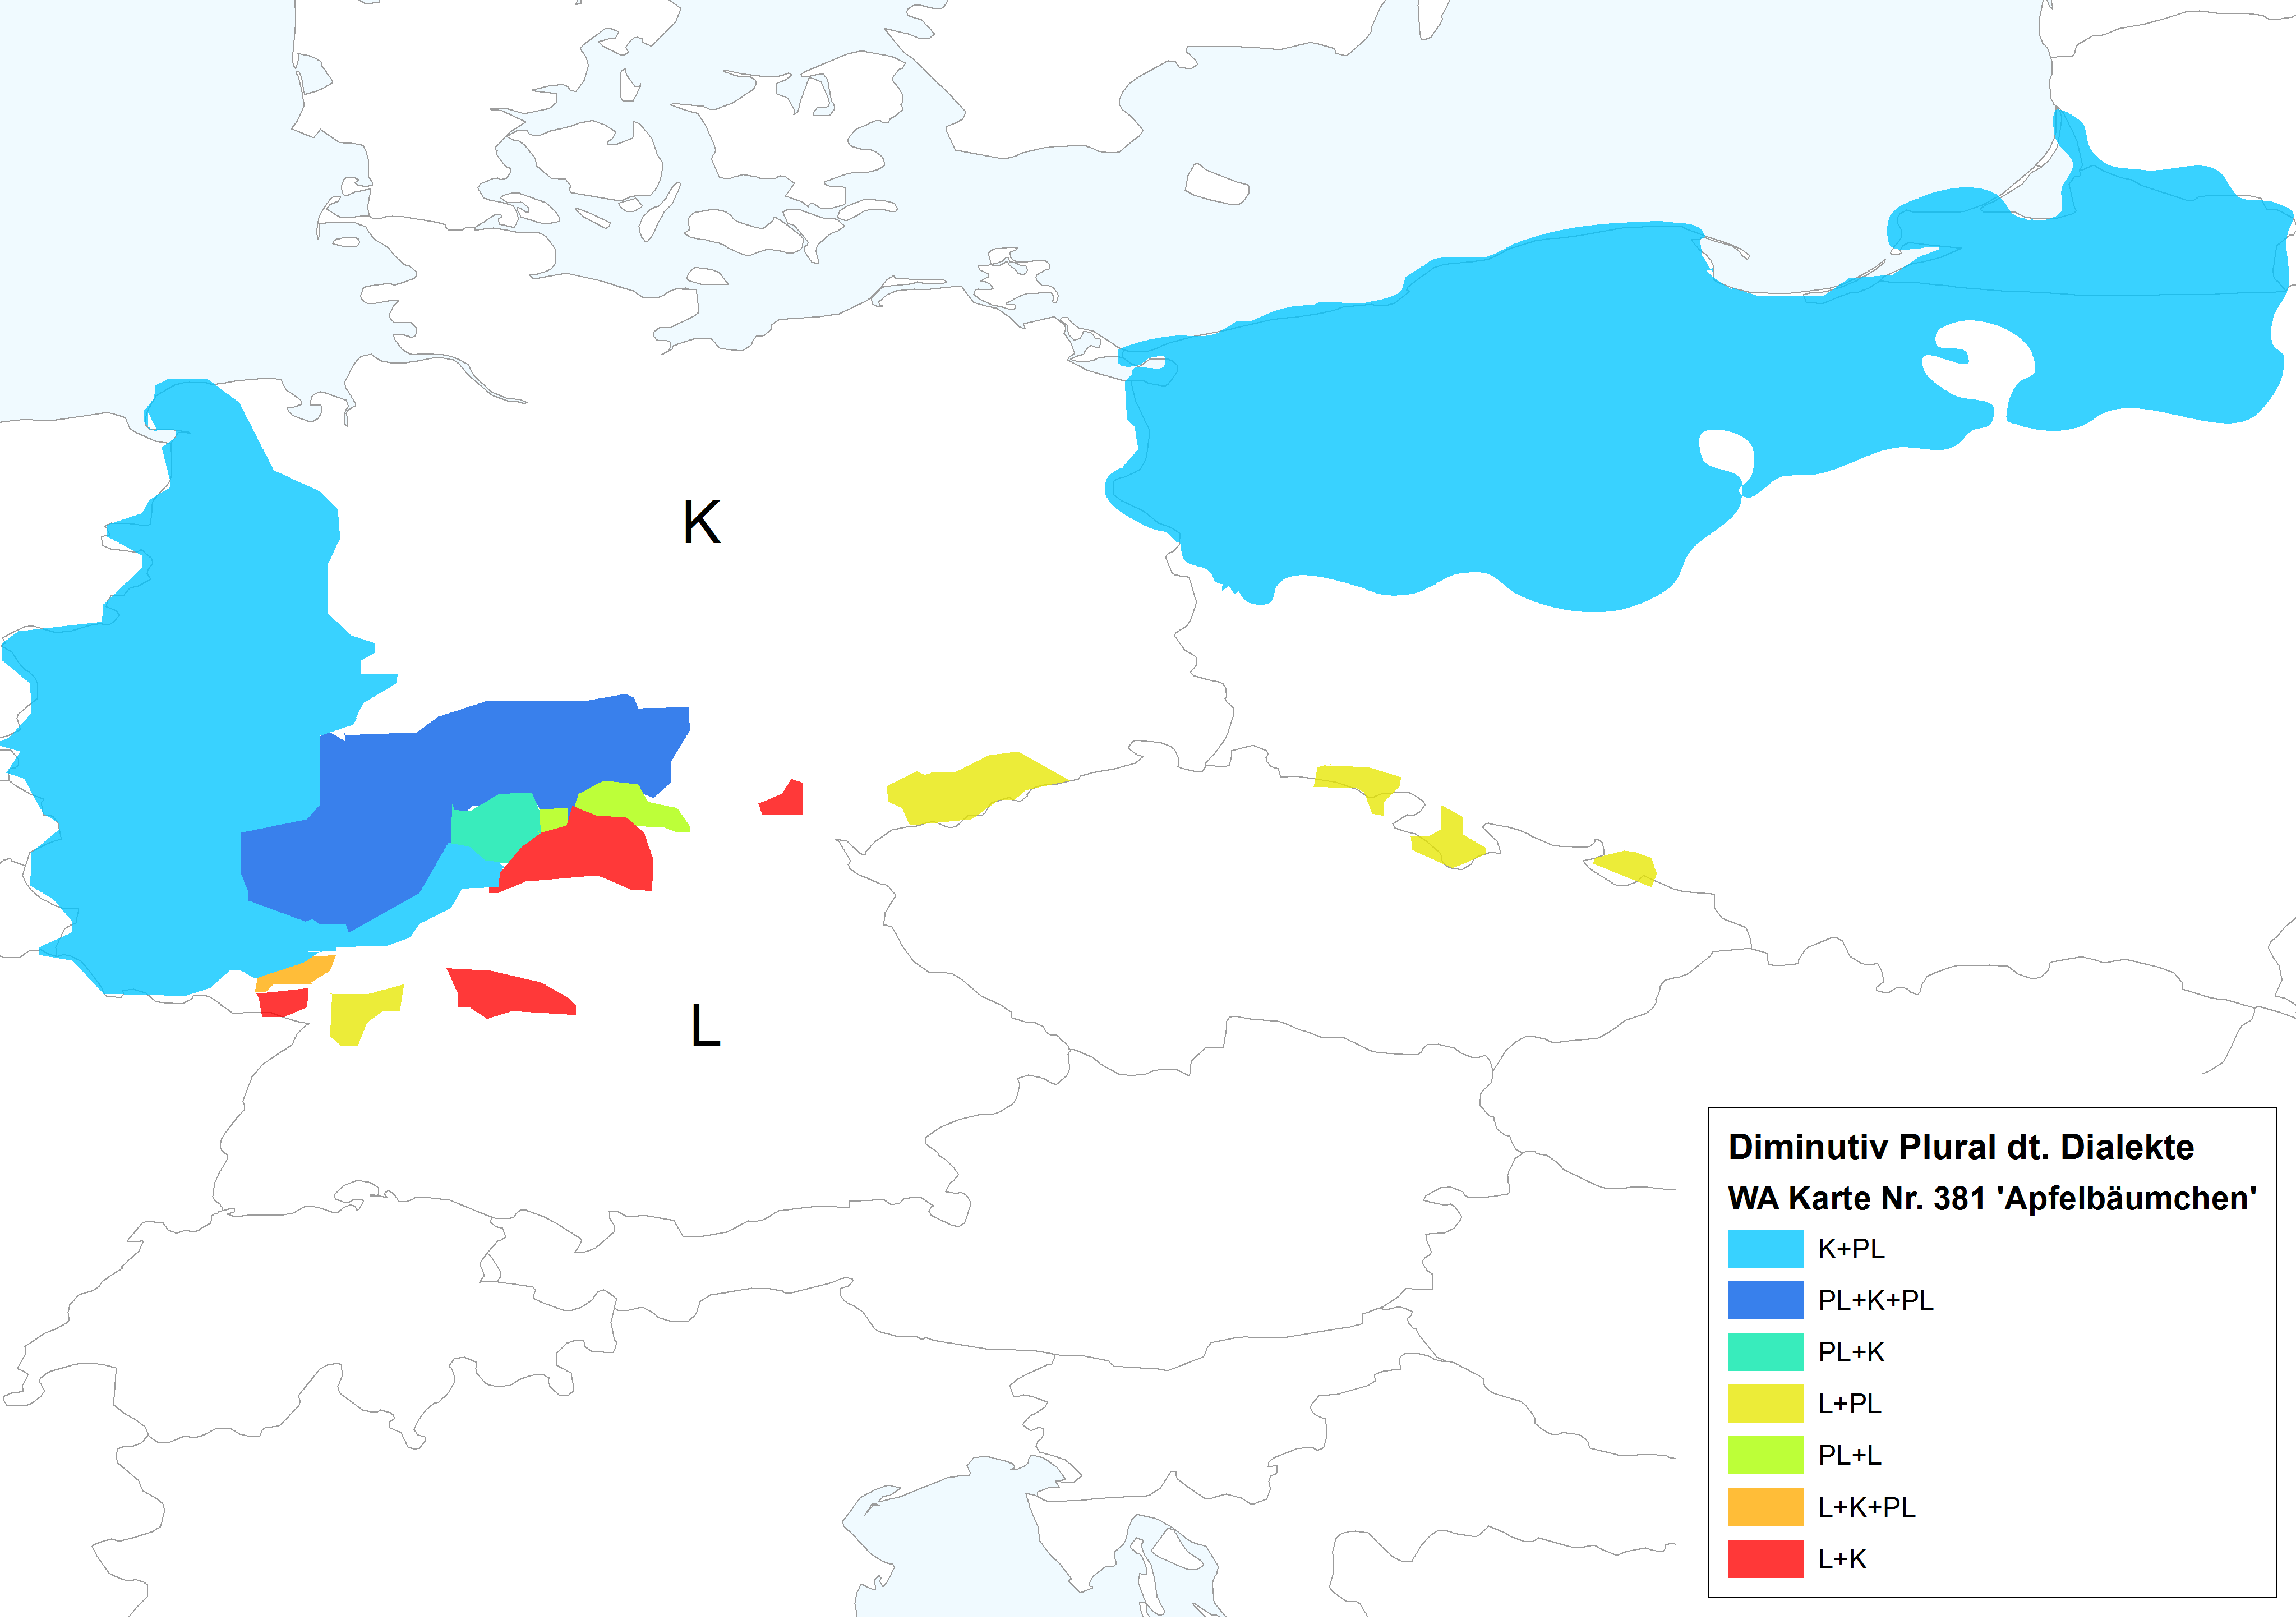
\includegraphics[width=\textwidth]{figures/DSA_DIM_PL_kurz.png}
		\caption{\label{DimDSA} Pluraldiminutionen in den dt. Dialekten (\hai{WA} Karte Nr. 381 \sem{Apfelbäumchen})}
		\end{figure}



\subsection{Diminution im Jiddischen}\label{dimJIDDISCH}
%  %\noindent

\largerpage[-2] 
Das Diminutionssystem des modernen Ostjiddischen fasst Tabelle  \ref{tblDIMOJ} zusammen. Der Singular wird mittels -\textit{l} (1. Grad) und -\textit{ele} (2. Grad)\footnote{Das Suffix -\textit{ele} findet sich auch bei auf /l/ auslautenden Nomina auch im 1. Grad, z.\,B.\, \RL{{{פ\makebox(-0.8,7)[r]{\libertineGlyph{uni207B}}}}ויגל} 
\textit{foygl} \sem{Vogel} \RL{{{פ\makebox(-0.8,7)[r]{\libertineGlyph{uni207B}}}}ייגעלע} 
\textit{feygele} \sem{Vogel\textsubscript{{\Dim} {\Sg}}}} gebildet (\citealt[69]{Jacobs2005}; \citealt[80]{Perlmutter1988}). Die Pluraldiminution wird mittels -\textit{lekh} (1. Grad) bzw. -\textit{elekh} (2. Grad) gebildet (\citealt[162–163]{Jacobs2005}; \citealt[80]{Perlmutter1988}). Bei Nomina mit \ili{hebräisch}-aramäischer \il{hebräisch} Wurzel findet sich oftmals eine doppelte  Pluralmarkierung, indem \textit{-(e)lekh} an das bereits im Plural stehende Nomen gehängt wird, wie z.\,B.\, in \RL{חסיד} \textit{khsid} \sem{Frommer\textsubscript{{\Sg}}} > \RL{חסידים} \textit{khsidim} \sem{Fromme\textsubscript{{\Pl}}} > \RL{חסידיםלעך} \textit{khsidimlekh} \sem{Frommer\textsubscript{{\Pl}+ {\Dim} {\Pl}}} (\citealt[163]{Jacobs2005}; \citealt{Perlmutter1988}). Dieselbe Situation lässt sich aber auch in einzelnen Lexemen der germanischen Komponente finden, z.\,B.\, in \RL{קינדערלעך} \textit{kinderlekh} \sem{Kind\textsubscript{{\Pl} + {\Dim} {\Pl}}} (\citealt[163]{Jacobs2005}; \citealt{Perlmutter1988}). Jiddisch orientiert sich damit an der \hai{L}-\isi{Diminution}, die im Ober- und Mitteldeutschen verbreitet ist. Das \isi{Pluralsuffix} findet sich in den deutschen Dialekten des Ost- und Rheinfränkischen als -\textit{lich} belegt, wo es sich entlang der Isoglosse zwischen \hai{L}- und \hai{K}-\isi{Diminution} als Fusionsform beider Formen herausgebildet hat (\citealt[647]{Grimm1890}; \citealt[245]{Weinhold1867}; \citealt[124]{Wrede1908}; \citealt[49]{Paul1920}).\footnote{Die Analyse des Suffixes als Fusion der zwei Basistypen von \isi{Diminution} wird nicht von jedem geteilt. Z.\,T. wird dieses Suffix als \isi{Komposition} von \hai{L}-\isi{Diminution} und dem Kollektivsuffix {\ahd} -\textit{ahi}, {\mhd} -\textit{ech} (-\textit{ach}, -\textit{ich}), nhd. -\textit{icht} (un\isi{produktiv} z.\,B.\, in \textit{Kehricht}, \textit{Dickicht}) analysiert, so etwa in \cite[484]{Schirmunski1962} oder \cite[110–112]{Timm2005}. \cite[235]{Weinhold1867} schlägt vor, dass die Existenz des Kollektivsuffixes als Katalysator für die Grammatikalisierung der Fusionsform als \isi{Pluralsuffix} gewirkt haben mag. Ebenso können auch die -\textit{ach}-Plurale des Oberdeutschen dazu beigetragen, der Fusionsform -\textit{lich} Pluralbedeutung zu geben (vgl.\, \citealt{Rowley1994}).}\\ 



 \begin{table}
%\begin{longtable}{ccc|ccc}

		\begin{tabular}{llllll}

	\lsptoprule

\textbf{Grad} &\textbf{Numerus} & \textbf{Suffix} & \multicolumn{2}{c}{\textbf{Beispiel \sem{Lied}}} \\ 
\midrule 

1. & {\Sg} & -\textit{l} & \RL{לידל} & \textit{lidl} &\sem{kleines Lied} \\

1. & {\Pl} & -\textit{lekh} & \RL{לידלעך}& \textit{lidlekh} &\sem{kleine Lieder} \\ %format?!   andere Zeilentrennung überlegen? \hdashline?

2. & {\Sg} & -\textit{ele} &  \RL{לידעלע} &\textit{lidele}& zärtlich \sem{Lied} \\ 

2. & {\Pl} & -\textit{elekh} &\RL{לידעלעך} &\textit{lidelekh}& zärtlich \sem{Lieder} \\
 
 
 
\lspbottomrule
 \end{tabular}
		 \caption{Das Diminutionssystem des standardisierten Ostjiddischen}
		 \label{tblDIMOJ}
		 \end{table}
		% \end{longtable}


Die Situation der \isi{Diminution} in den jiddischen Dialekten ist bislang noch nicht beschrieben worden. Die Daten des \hai{LCAAJ} (\citeyear[120]{Herzog2000}) lassen vermuten, dass es tatsächlich diatopisch unterschiedliche Suffixe gab und womöglich auch das System der graduellen Diminuierung de facto nicht soweit verbreitet war, wie das standardisierte Jiddisch vermuten lässt.\footnote{Die Daten zur \isi{Diminution} des \hai{LCAAJ} (\citeyear[120–125, insbes. Karte 36]{Herzog2000}) bieten nur einen minimalen Ausschnitt in die tatsächliche Sprachsituation. Dies zeigt sich besonders daran, dass hier im Singular zwei unterschiedliche und nicht miteinander vergleichbare Suffixe (\RL{שיקסע} \textit{shikse} \sem{Nichtjüdin} im Westjiddischen und \RL{מויל} \textit{moyl} \sem{Mund} im Ostjiddischen) die Basis bilden. Wie \cite{Wrede1908} zeigt, ist die Wahl eines Diminutivsuffixes stark lexemgebunden, vgl.\, S.\, \pageref{wredeDIM}. Hinzu kommt, dass die Erhebungsmethode des Fragebogens im Westjiddischen kaum dazu ausreichte,  semantische Feinheiten wie die \isi{Diminution} 1. und 2. Grades einzufangen.} Dialektale Abweichungen vom Standard finden sich zum Beispiel im \hai{{\NOJ}}, wo die Singulardiminuierung von  \RL{מויל} \textit{moyl} \sem{Mund}  mittels -\textit{kh(e)le} erfolgt, und im \hai{{\SOJ}} findet sich das Suffix -\textit{lche(n)} im Lexem \RL{שיקסע} \textit{shikse} \sem{Nichtjüdin} (\citealt[122, Karten Nr. 36S1, 36S2]{Herzog2000}). \,%rs + "Nr."
Wie in den deutschen Dialekten herrscht so scheinbar auch in den jiddischen Varietäten eine vom Lexem abhängige Vielfalt an Diminutivsuffixen vor (vgl.\, S.\, \pageref{wredeDIM}). Vor allem aber fällt die Datenmenge des \hai{LCAAJ} zu gering aus, als dass sich auf deren Basis Aussagen über das jiddische Diminutionssystem machen ließen.\label{SOJDIM}

Dies zeigt sich besonders im Westjiddischen. Den Daten des \hai{LCAAJ} (\citeyear[120–125]{Herzog2000}) zufolge bildet das Westjiddische die Singulardiminution im \hai{{\SWJ}} und südwestlichen \hai{{\ZWJ}} mittels -\textit{(e)le}, im \hai{{\NWJ}} und \hai{{\NÜJ}} mittels -\textit{l}, im \hai{{\SÜJ}} finden sich beide Suffixe parallel und im westlichen \hai{{\ZWJ}} ist -\textit{che(n)} zu finden (\citealt[120–122, Karten Nr. 36, Nr. 36S1]{Herzog2000}). \citeauthor{GuggenheimGruenberg1973}s Daten zum südlichen \hai{{\SWJ}} und \hai{{\ZWJ}} bestätigen dieses Bild nicht; vielmehr finden sich hier die den koterritorialen deutschen Dialekten entsprechenden Suffixe (\citealt[92, Karte Nr. 33]{GuggenheimGruenberg1973}). Dieses Bild bestätigen auch schriftliche Quellen aus dem 19. und 20. Jahrhundert. So findet sich im Westjiddischen nördlich des Mains die \hai{K}-\isi{Diminution} (\ref{BspSGWJ1}–\ref{BspSGWJ3}) und im Süden \hai{L}-\isi{Diminution} (\ref{BspSGWJ4}–\ref{BspSGWJ6}). \label{DIMSGWJ}

 \eenumsentence{
 
 \item \textit{Stickche} \sem{Stück\textsubscript{{\Dim} {\Sg}}}  \\
 \textit{Schnüpfche} \sem{Schnupfen\textsubscript{{\Dim} {\Sg}}} \\
(\qu{Das verfrühte Schulenrufen} Aurich 1902 [\citealt[67]{Reershemius2007}])  \label{BspSGWJ1}
 
  \item \textit{Goichen} \sem{Nichtjude\textsubscript{{\Dim} {\Sg}}} \\
  (\qu{Die Lebenserinnerungen des A. H. Heymann}, Strausberg (Berlin), 1909:\,92 [\citealt[39]{Schaefer2010}])  \label{BspSGWJ2}


 \item \RL{תמרכה} \textit{tamarche} \sem{Tamara\textsubscript{{\Dim} {\Sg}}} \\
 \RL{גומפלכה}  \textit{gumplche} \sem{Gumpel\textsubscript{{\Dim} {\Sg}}} \\
 (\qu{Die Hochzeit zu Grobsdorf} 1822:\,dramatis personae) \label{BspSGWJ3}
 
  
   \item \textit{Großvaterle} \sem{Großvater\textsubscript{{\Dim} {\Sg}}}  \\
   (\qu{Die Juden von Zirndorf} Fürth, 1897 [1996]:\,177)\label{BspSGWJ4}
   
    \item \textit{Stickle} \sem{Stück\textsubscript{{\Dim} {\Sg}}}  \\
    \textit{Peckle} \sem{Packet\textsubscript{{\Dim} {\Sg}}}  \\
      (\qu{Garkisch} Mulhouse, 1930:\, 9; 20) \label{BspSGWJ5}
      
            
    \item \textit{Stickl} \sem{Stück\textsubscript{{\Dim} {\Sg}}}  \\
     \textit{Majerl} \sem{Mauer\textsubscript{{\Dim} {\Sg}}}  \\
 (Wenkerbogen aus Frauenkirchen Nr. 42663/300447; vgl.\, \citealt{FleischerSchaeferErsch}) \label{BspSGWJ6}
 
 }

Der \hai{LCAAJ} erweckt mit der einzigen Kartierung eines durchaus problematischen\footnote{Problematisch an diesem Lexem als Stellvertreter der Pluraldiminution ist, dass die \isi{Diminution} bereits erstarrt sprich lexikalisiert, sein könnte. vgl.\, dazu auch den westjiddischen Beleg in (\ref{bspDIMPLlichAURICH}) S.\, \pageref{bspDIMPLlichAURICH} (\citealt[133]{Reershemius2007}).} 
Lexems mit Pluraldiminution \RL{קרעפלעך} \textit{kreplekh} \sem{Knödel\textsubscript{{\Dim} {\Pl}}} den falschen Eindruck, dass das Westjiddische über keine vom Singular distinkte Pluraldiminution wie das Ostjiddische verfügt. Der westlichste Beleg für die \isi{Diminution} mittels -\textit{lekh} im \hai{LCAAJ} findet sich in Prag. Dies ist ein besonders eindrucksvolles Beispiel für die Unzulänglichkeit der westjiddischen Daten des \hai{LCAAJ}, denn selbst \cite[94, Karte Nr. 34]{GuggenheimGruenberg1973} gelingt es, die westjiddische Pluraldiminution mittels -\textit{lich} einzufangen. \cite[56]{Zuckerman1969}, dessen Daten eigentlich in die Kartierung des \hai{LCAAJ} hätten einfließen müssen, findet dieses Suffix im Elsässer Jiddisch. Die ersten Belege für Pluraldiminutivbildungen auf -\textit{lich} sind aus dem Mitteljiddischen, d.\,h. aus dem 15. bis 17. Jahrhundert, bekannt (\citealt[112]{Timm2005}). Das historische Diminutivsystem des Jiddischen zeigt noch generell eine hohe Vielfalt der Suffixe (\citealt[109–113]{Timm2005}). Damit ist anzunehmen, dass das moderne System, wie es Tabelle \ref{tblDIMOJ} zeigt, tatsächlich eine Idealisierung eines wahrscheinlich wesentlich komplexeren Systems darstellt. Tatsächlich lässt sich im Fall der Pluraldiminution ein Ost-West-Gefälle innerhalb des jiddischen Dialektgebiets erkennen: Aus dem Westjiddischen sind uns bislang lediglich Quellen mit dem Suffix -\textit{lich}/-\textit{lisch} (\ref{bspDIMPLlich}–\ref{bspDIMPLlisch}) überliefert, im \hai{{\NÜJ}} findet sich vereinzelt das Suffix -\textit{lech} (\ref{bspDIMPLlechHeymann}–\ref{bspDIMPLlech}) und im \hai{{\SÜJ}} und südwestjiddischen Randgebieten zum \hai{{\SÜJ}} -\textit{loch} und -\textit{lach} (\ref{bspDIMPLloch}–\ref{bspDIMPLlach}). Allem Anschein nach ist also die Wahl des Vokals eine regional variierende Komponente. Hinzu kommt, dass im Westjiddischen nördlich des Mains das sonst für das Jiddische übliche \isi{Pluralsuffix} -\textit{l}- +  Vokal + -\textit{ch} nur in zwei umstrittenen Belegen vorliegt.\footnote{Diese beiden Belege sind in den  (\ref{bspDIMPLlichAURICH}) u. (\ref{bspDIMPLlechHeymann}) angeführt. Der Beleg aus Aurich kann, wie \citet[133 Fn. 199]{Reershemius2007} anführt, als ostjiddisches \isi{Lehnwort} im Diminutiv Plural erstarrt sein. Ebenfalls ein ostjiddischer Einfluss ist im Beleg aus Strausberg möglich, da auch dieses Lexem nicht im Westjiddischen belegt ist, vgl.\, \cite[40f]{Schaefer2010}. Die Wahl des Vokals im Diminutivsuffix spricht jedoch in beiden Fällen dafür, dass hier eine regionale Form vorliegt und nicht eine aus dem Ostjiddischen entlehnte.} Das allgemeine Bild westjiddischer (Plural-)\isi{Diminution} im Norden des Sprachgebiets scheint eine größere Variation zu haben, als es im Südwesten der Fall ist. Ein eindrucksvolles und glaubwürdiges Beispiel ist hier \qu{Die Hochzeit zu Grobsdorf}, in der eine hohe Varianz an Diminutivsuffixen im Plural\footnote{Im Singular findet sich hier regulär \RL{כה}- \textit{-che}. Die Pluralsuffixe, wie auch das Singularsuffix, können selbstverständlich aus dem Kontakt zu den koterritorialen hessischen Dialekten ins örtliche Jiddisch Eingang gefunden haben, da dort eben solche Suffixe gebräuchlich sind, vgl.\, \hai{WA} Karten Nr. 381, 440; \cite[86]{Friebertshaeuser1987}.} vorliegt (\ref{bspDIMPLgrob}). Wichtig ist festzuhalten, dass kein im Jiddischen vorkommendes Suffix auch in einem deutschen Dialekt belegt ist.\footnote{Es besteht selbstverständlich die generelle Möglichkeit, dass im Ostjiddischen \isi{Diminution} auch mittels slawischer Suffixe (insbes. -\textit{ke}) gebildet werden können. Eine umfassende Untersuchung zum ostjiddischen Diminuierungssystem müsste diesen Fall zumindest berücksichtigen, da das Suffix selbst (wenn auch un\isi{produktiv}) in vielen Lexemen der slawischen  Komponente vorhanden ist, z.\,B.\, \RL{קא\makebox(-1.5,-6.5)[r]{\libertineGlyph{uni207B}}טשקע} \textit{katshke} \sem{Ente} (vgl.\, {\poln} \textit{kaczka} \sem{Ente}), \RL{מא\makebox(-1.5,-6.5)[r]{\libertineGlyph{uni207B}}רגעריטקע} \textit{margeritke} \sem{Gänseblümchen} (vgl.\, {\poln} \textit{margerytka} \sem{Gänseblümchen}).} 


 \eenumsentence{

\item \RL{מא\makebox(-1.5,-7.5)[r]{\libertineGlyph{uni207B}}דליך} \textit{madlich} \sem{Mädchen\textsubscript{{\Dim} {\Pl}}} \\
\RL{הורג-ליך} \textit{horeg-lich} \sem{Zwerg\textsubscript{{\Dim} {\Pl}}}\\
(\qu{Esther. Oder die belohnte Tugend} Fürth, 1854:\, 7; 17) \label{bspDIMPLlich} 

\item \textit{Kneidlich} \sem{Knödel\textsubscript{{\Dim} {\Pl}}} \\
(\qu{Das verfrühte Schulenrufen} Aurich 1902:\,3. Auftritt [\citealt[133]{Reershemius2007}]) \label{bspDIMPLlichAURICH}

 \item \textit{Blimlisch} \sem{Blumen\textsubscript{{\Dim} {\Pl}}}\\
  \textit{Sticklisch} \sem{Stücke\textsubscript{{\Dim} {\Pl}}} \\
  (\qu{Garkisch} Mulhouse, 1930:\, 15; 16) \label{bspDIMPLlisch}
 
\newpage 
 \item \textit{Rendlech} \sem{Münze\textsubscript{{\Dim} {\Pl}}} \\
 (\qu{Die Lebenserinnerungen des A. H. Heymann}, Strausberg (Berlin), 1909:\,5  [\citealt[40]{Schaefer2010}])  \label{bspDIMPLlechHeymann}
 
 \item \textit{Bäumlēch} \sem{Baum\textsubscript{{\Dim} {\Pl}}} \\
  \textit{Äpelech} \sem{Apfel\textsubscript{{\Dim} {\Pl}}} \\
 (Wenkerbogen aus Kobyla Góra Nr. 09746; vgl.\, \citealt{FleischerSchaeferErsch}) \label{bspDIMPLlech}
 
 \item \textit{Schefeloch} \sem{Schaf\textsubscript{{\Dim} {\Pl}}}\\
  \textit{Eppeloch} \sem{Apfel\textsubscript{{\Dim} {\Pl}}} \\
 (Wenkerbogen aus Frauenkirchen Nr. 42663/300447; vgl.\, \citealt{FleischerSchaeferErsch}) \label{bspDIMPLloch}

 \item \textit{Kinderlach}  \sem{Kind\textsubscript{{\Dim} {\Pl}}}\\
  \textit{Bondlach}  \sem{Bund\textsubscript{{\Dim} {\Pl}}}\\
(\qu{Torres Lokschen} Budapest, 1900:\, 39, 49; 40) \label{bspDIMPLlach}

 \item \RL{מערערכער} \textit{merercher} \sem{Mädchen\textsubscript{{\Dim} {\Pl}}} \\
 (\qu{Die Hochzeit zu Grobsdorf} 1822:\,14, 110)\\
 \RL{קערלכה} \textit{kerlche} \sem{Kerl\textsubscript{{\Dim} {\Pl}}}\\
 (\qu{Die Hochzeit zu Grobsdorf} 1822:\,37) \label{bspDIMPLgrob} 
 
 }

 \subsection{Diminution im \hai{chrLiJi1}}\label{dimsg}
  %  %\noindent
 
Wie eingangs erwähnt (S.\,\pageref{AnzahlDIM}) liegt im \hai{chrLiJi1} eine Vielzahl an Suffixen zur Singulardiminution vor, die im einzelnen mit Beispielbelegen versehen in Tabelle \ref{tblDIMSG} angeführt sind. An erster Stelle steht das Suffix -\textit{che(n)}, wie es auch in der deutschen Schriftsprache Verwendung findet. In diesen Fällen erfolgt also die Markierung der jüdischen Figuren weniger über die Abweichung von der schriftsprachlichen Norm, als durch eine auffallend häufige Verwendung der \isi{Diminution}.\footnote{Um gesicherte Aussagen über die \isi{Frequenz} von Diminutiva im Text jüdischer Figurenrede im Vergleich zu nicht-jüdischer Figuren zu machen, reichen die hier erhobenen Daten selbstverständlich nicht aus. Die Feststellung, dass \isi{Diminution} im Text  jüdischer Figuren die übliche \isi{Frequenz} von \isi{Diminution} übersteigt, beruht hier lediglich auf der Leseerfahrung der Verfasserin.} In zwölf Quellen und damit zweithäufigstes Suffix ist -\textit{el}. Dieses Suffix tritt in den deutschen Dialekten in kleinen Teilen des Niederalemannischen, Rheinfränkischen, Obersächsischen und Schlesischen auf (\hai{WA} Karte Nr. 440) und entspricht der ostjiddischen Singulardiminution des 1. Grads (s. Tabelle \ref{tblDIMOJ}, S.\, \pageref{tblDIMOJ}). Das Suffix -\textit{ele}, welches den 2. Grad der Singulardiminution im Ostjiddischen bildet, findet sich in nur zwei Quellen des \hai{chrLiJi1}. Mit einer Belegzahl von zehn Quellen ebenfalls sehr häufig ist die Fusionsform -\textit{elche(n)}. Diese ist in hessischen, rhein- und moselfränkischen Dialekten weit verbreitet (\hai{WA} Karte Nr. 440). 


  \begin{table}[t]
%\begin{longtable}{ccc|ccc}
%
		\begin{tabularx}{\columnwidth}{lXr}

\lsptoprule

\textbf{Suffix} &\textbf{Beispiel} & \textbf{Quellen} \\ \midrule 


\textit{-che(n)} & \textit{Doktor-Titelche} \sem{Doktortitel\textsubscript{{\Dim} {\Sg}}} (\hai{PG}:\,3), \textit{Doktorche} \sem{Doktor\textsubscript{{\Dim} {\Sg}} } (\hai{JK}:\,4, 5, 8), \textit{Pferdchen} \sem{Pferd\textsubscript{{\Dim} {\Sg}}} (\hai{JP}:\,5) & 28 \\ 

 
 \textit{-ge} & \textit{Biksge} \sem{Büchse\textsubscript{{\Dim} {\Sg}}} (\hai{PA}:\,9),  \textit{Stückge} \sem{Stück\textsubscript{{\Dim} {\Sg}}} (\hai{PA}:\,34) & 1 \\ 
  
 \textit{-je} & \textit{Musje } \sem{Maus\textsubscript{{\Dim} {\Sg}}} (\hai{{\PP}}:\,30) & 1\\

 \textit{-ke} & \textit{Britschke } \sem{Pritsche\textsubscript{{\Dim} {\Sg}}} (\hai{AJ}:\,6),  \textit{Marieken} \sem{Marie \textsubscript{{\Dim} {\Sg}}} (\hai{DP}:\,27) & 2 \\
 
 \textit{-elche(n)} & \textit{Wechselche } \sem{Wechsel\textsubscript{{\Dim} {\Sg}}} (\hai{PA}:\,11),  \textit{Ringelche } \sem{Ring \textsubscript{{\Dim} {\Sg}}} (\hai{WA}:\,165),  \textit{Ringelchen } \sem{ Ring\textsubscript{{\Dim} {\Sg}}} (\hai{FS}:\,44) & 10 \\
 

 \textit{-elgen} & \textit{Mägelgen} \sem{Magen\textsubscript{{\Dim} {\Sg}}} (\hai{OF}:\,1) & 1 \\
 
 \textit{-lach} & \textit{Stickelach} \sem{Stück\textsubscript{{\Dim} {\Sg}}} (\hai{SS}:\,10) &1 \\
 
 \textit{-lich} & \textit{Hütlich} \sem{Hut\textsubscript{{\Dim} {\Sg}}} (\hai{SV}:\,3),  \textit{Hälslich} \sem{Hals\textsubscript{{\Dim} {\Sg}}} (\hai{LM}:\,22),  \textit{Sußlich} \sem{Pferd\textsubscript{{\Dim} {\Sg}}} (\hai{GP} Nürnberg, 1831:\,35, 36), \textit{Lämmlich} \sem{Lamm} (\hai{PG}:\,11) & 4\\
 
 \textit{-lein} & \textit{Stücklein } \sem{Stück\textsubscript{{\Dim} {\Sg}}} (\hai{HJ}:\,101),  \textit{Büchlein} \sem{ Buch\textsubscript{{\Dim} {\Sg}}} (\hai{LM}:\,12) & 2\\
 
 \textit{-le} & \textit{Bäuerle } \sem{Bauer\textsubscript{{\Dim} {\Sg}}} (\hai{PA}:\,)VIII,  \textit{Davidle} \sem{ David\textsubscript{{\Dim} {\Sg}}} (\hai{OF}:\,2),  \textit{Schwesterle } \sem{ Schwester\textsubscript{{\Dim} {\Sg}}} (\hai{AK}:\,247) & 7\\
 
 \textit{-el} & \textit{Bauernmädel} \sem{Bauernmädchen\textsubscript{{\Dim} {\Sg}}} (\hai{{\PP}}:\,21),  \textit{Päckel} \sem{Packet\textsubscript{{\Dim} {\Sg}}} (\hai{FE}:\,56),  \textit{Schicksel} \sem{Nichtjüdin\textsubscript{{\Dim} {\Sg}}} (\hai{JP}:\,5) & 12\\

 \textit{-ele} & \textit{Mouschele} \sem{Mose\textsubscript{{\Dim} {\Sg}}} (\hai{OF}:\,2),  \textit{Patschhäntele} \sem{Patschehand \textsubscript{{\Dim} {\Sg}}} (\hai{GW}:\,13) & 2\\
 
\lspbottomrule
 \end{tabularx}
		 \caption{Diminutivsuffixe Singular im \hai{chrLiJi1}}
		 \label{tblDIMSG}
		 \end{table}


Die Darstellung der Einzelformen in Abbildung \ref{SgDimliji} zeigt, dass einzelne Suffixe in bestimmten Gebieten besonders häufig auftreten. So etwa das Suffix \textit{-el}, welches neben zwei Belegen aus Bonn, vor allem im Nordosten und im Südosten und damit in Kontaktzonen zum Ostjiddischen zu finden ist. Es könnte sich dabei um eine \isi{Emulation} des ostjiddischen Singularsuffix des 2. Diminutionsgrades \textit{-ele} handeln. Ebenfalls räumlich auffällig verhalten sich die Belege des Suffix \textit{-elche(n)}, welches wir zwar besonders im westmitteldeutschen Raum finden, wo es auch in den deutschen Dialekten verbreitet ist (vgl.\, Karte in Abbildung \ref{SgDimDSAliji}), allerdings ist es auch im Nordosten vielfach belegt, wo es für die deutschen Dialekte untypisch ist. 

   \begin{figure}[t]

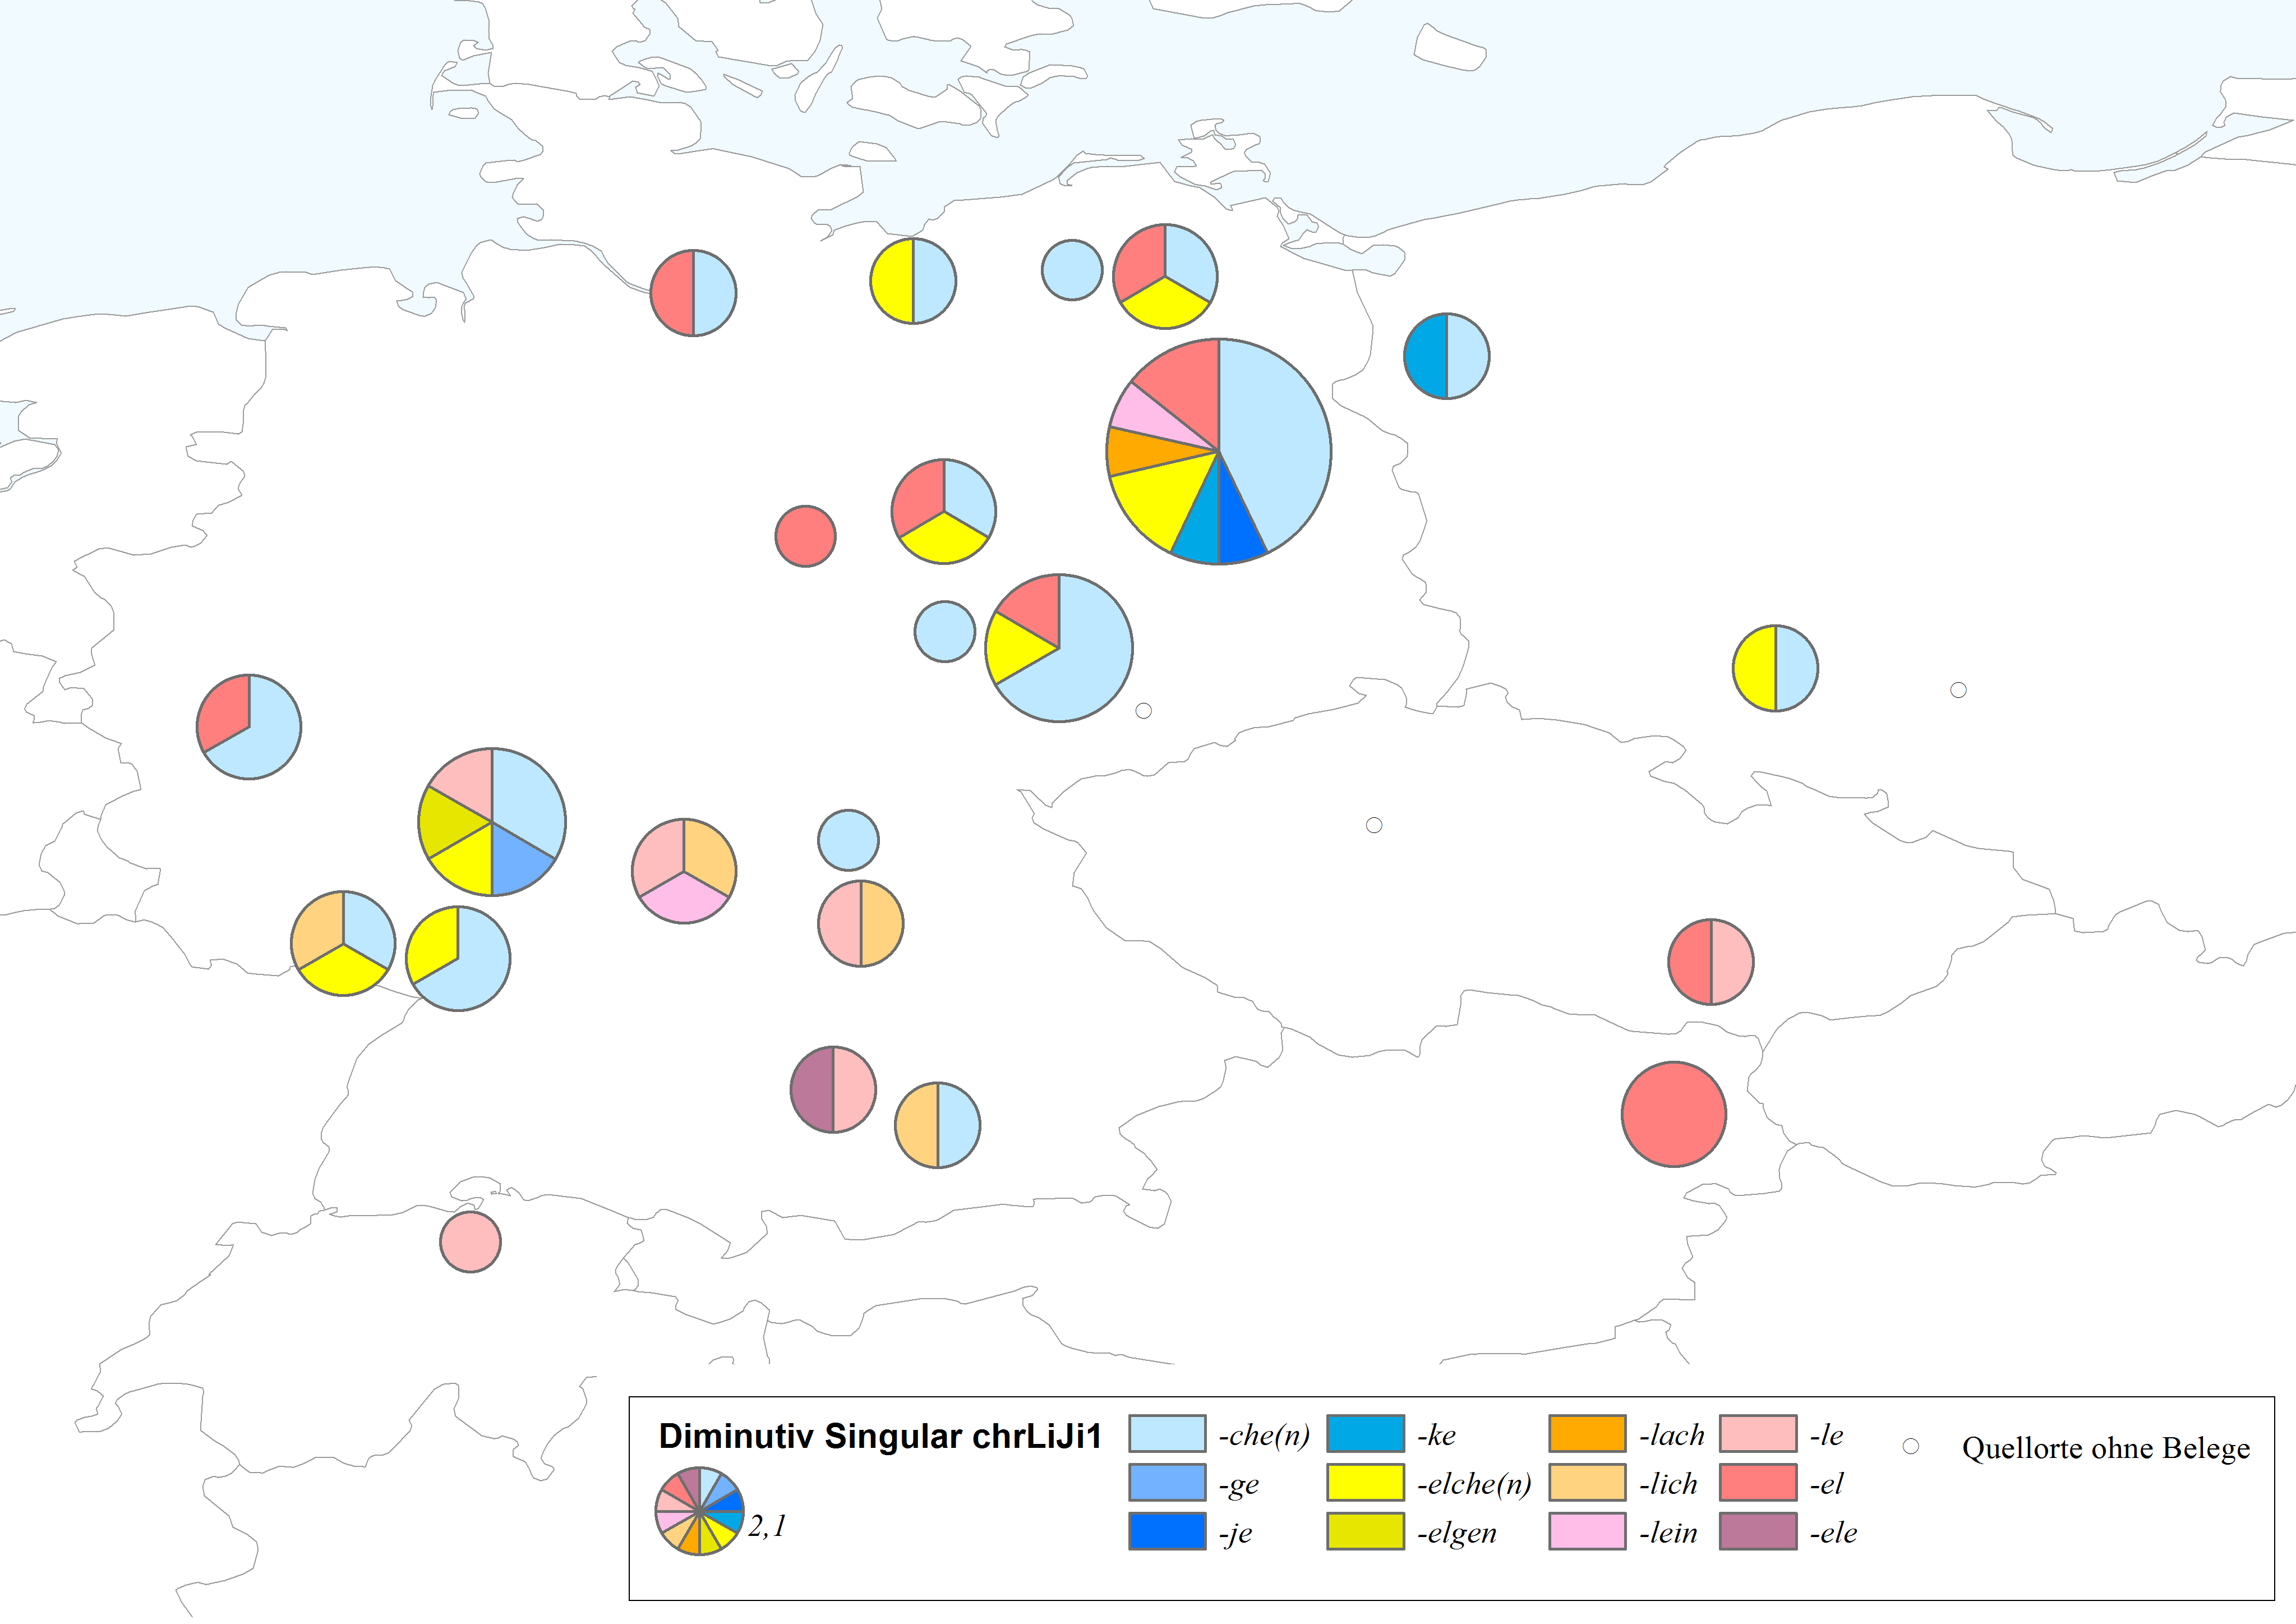
\includegraphics[width=\textwidth]{figures/DIM_SG.png}
		\caption{\label{SgDimliji} Singulardiminutionen im \hai{chrLiJi1}}
		\end{figure} 
 

\begin{figure} 

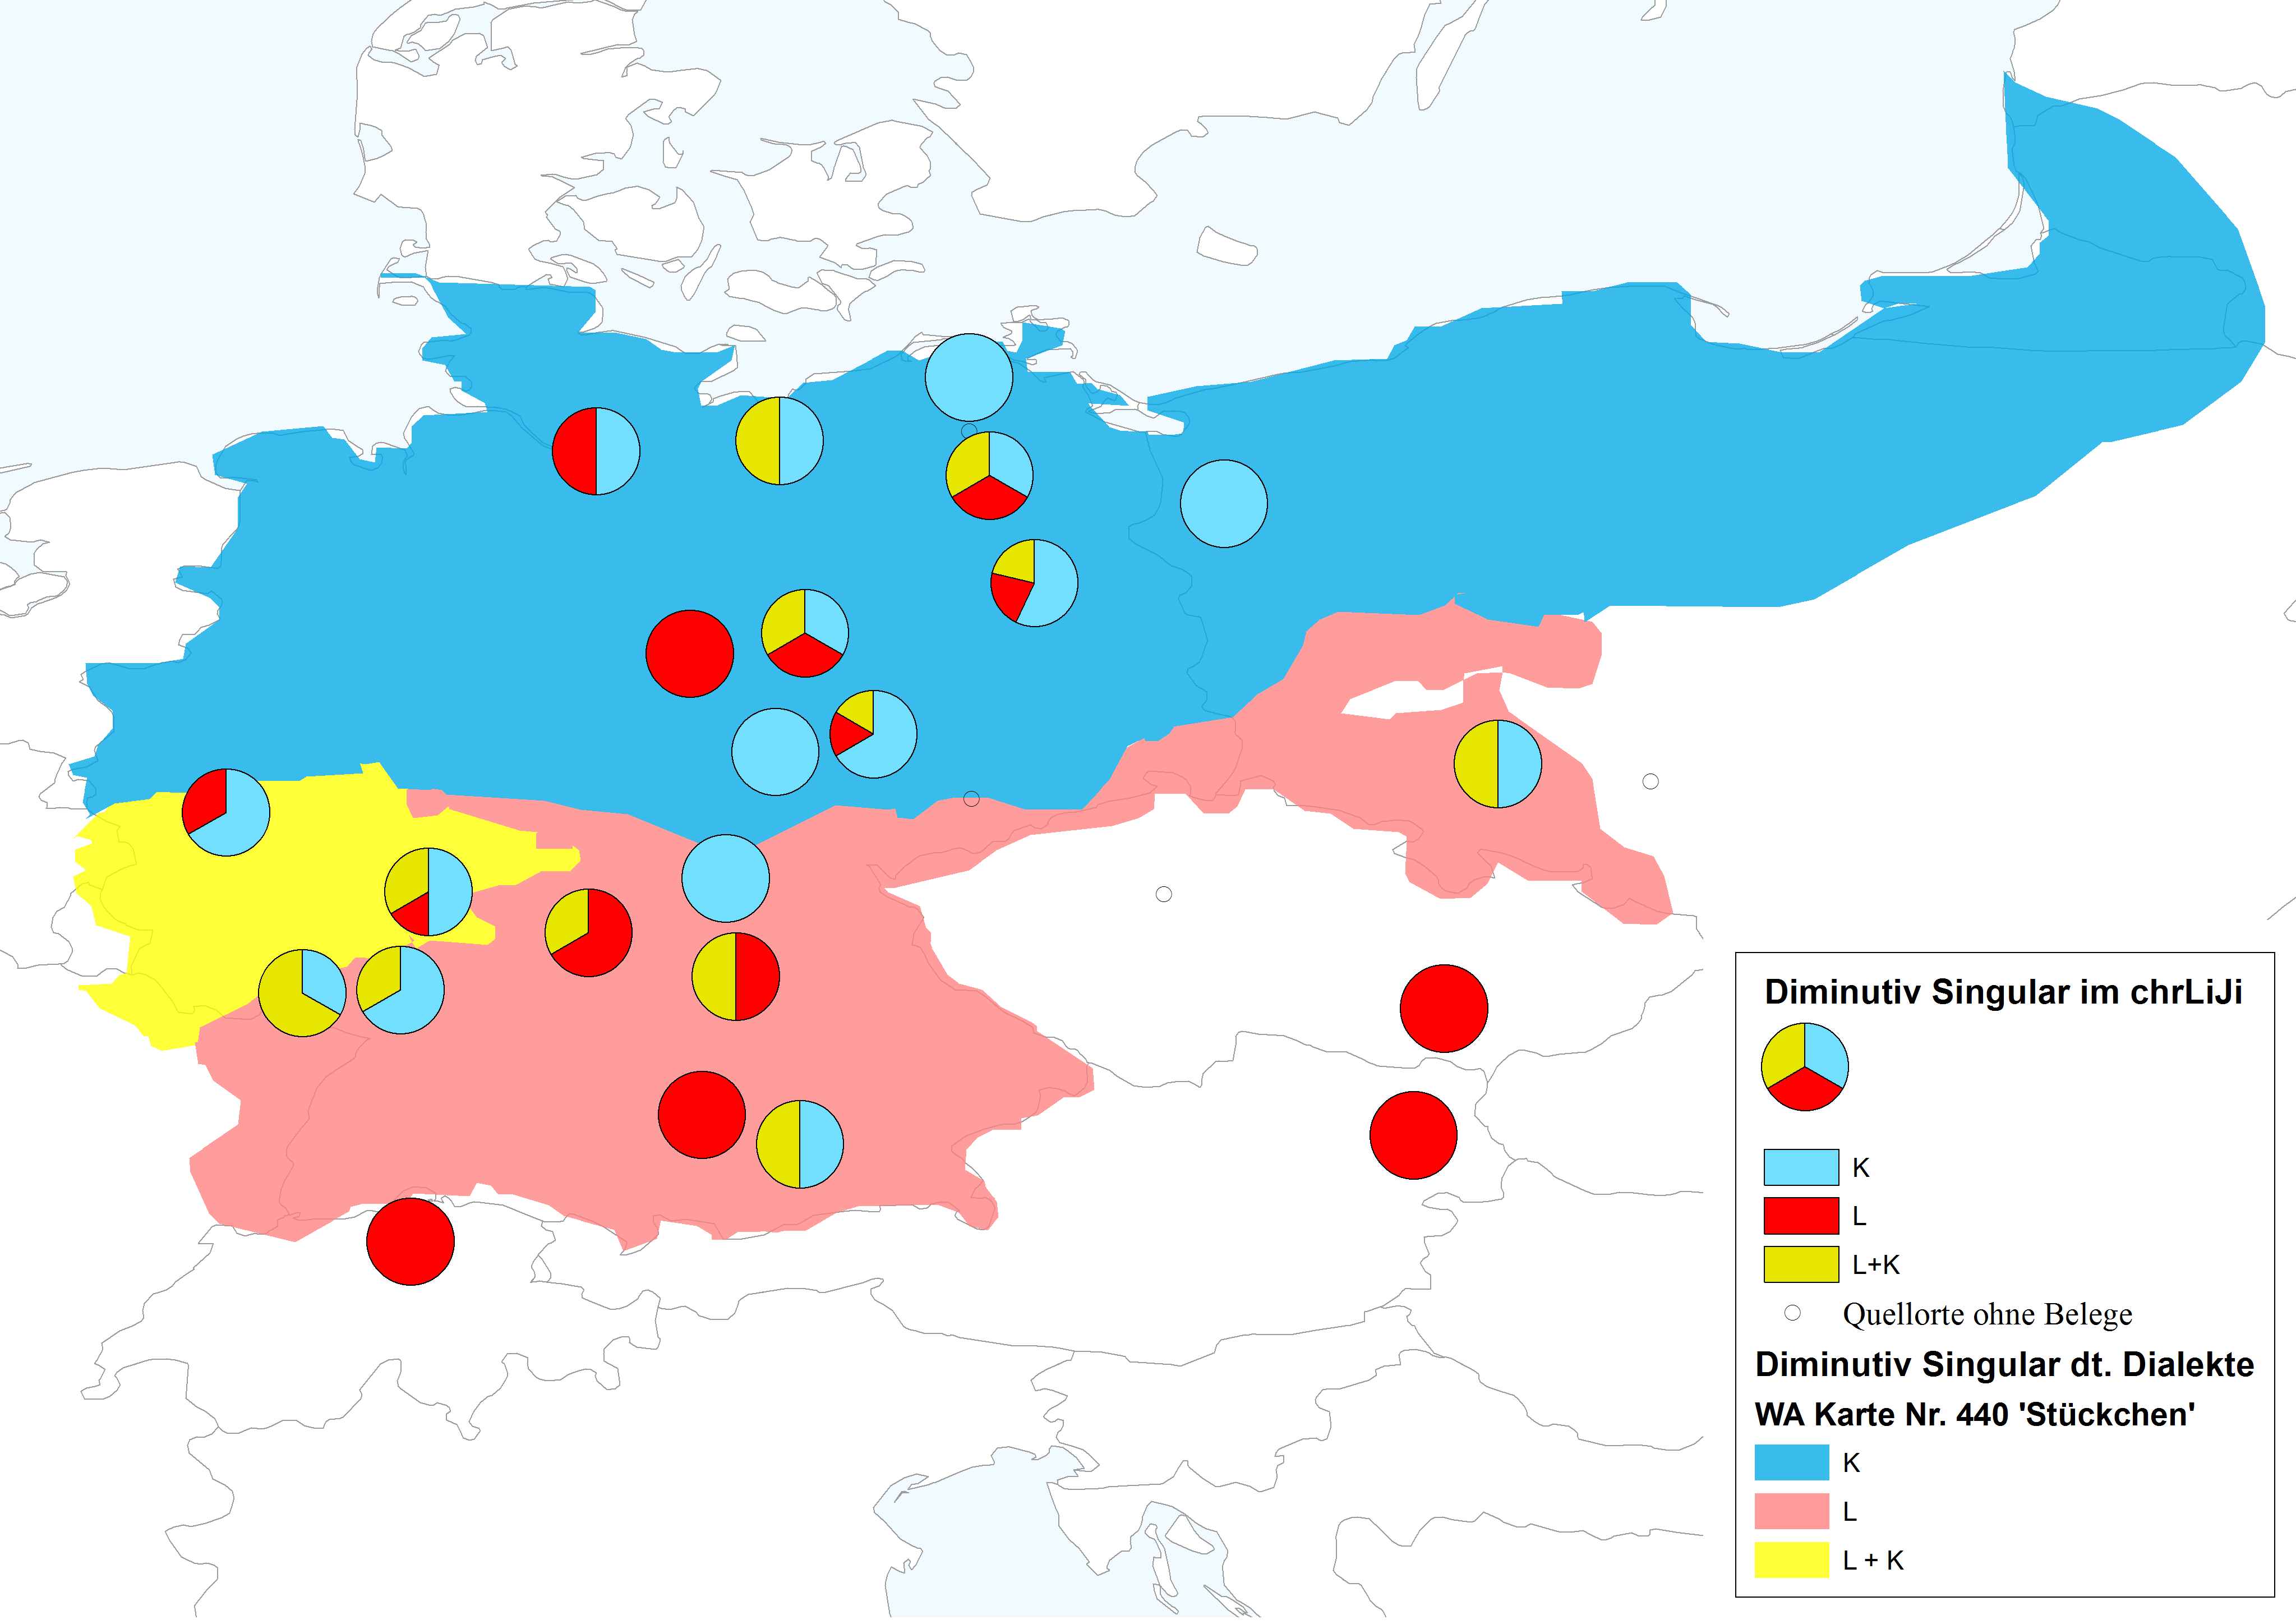
\includegraphics[width=\textwidth]{figures/DIM_SG_DSA_DIM_SG_kurz.png}
		\caption{\label{SgDimDSAliji} Singulardiminutionen im \hai{chrLiJi1} und den dt. Dialekten (\hai{WA} Karte Nr. 440 \sem{Stückchen}) }
		\end{figure}
 
Vier Quellen zeigen das Pluraldiminutivsuffix -\textit{lich} im Singular (s. Abbildung \ref{DimDSALiJilich}, S.\, \pageref{DimDSALiJilich}). Eine solche Verwendung dieses Suffixes im Singular ist weder aus jiddischen noch aus deutschen Varietäten bekannt. Da all diese Quellen das Suffix auch \quein{korrekt} bei der \isi{Diminution} Plural einsetzen, ist anzunehmen, dass es sich hierbei um Übergeneralisierungen handelt.\label{lichHyper} Den meisten Autoren des \hai{chrLiJi1} mag also nicht bewusst gewesen sein, dass das Jiddische eine Unterscheidung zwischen Diminutiv Singular und Plural trifft, und so wurde das  \isi{Pluralsuffix} auf den Singular übertragen.\footnote{Hinzukommt, dass mindestens ein Text durch die Schriften Itzig Veitel Sterns (pseud.) (\hai{GP}  Nürnberg, 1831) beeinflusst ist, welcher -\textit{lich} sowohl im Singular als auch im Plural verwendet; zumindest nennt der Verfasser von \hai{PG} (Speyer, 1835) im Vorwort diesen als sein Vorbild (vgl.\, Abschnitt \ref{IVS}, S.\, \pageref{IVS}).} 
 
Die Kartierung der Daten in den Abbildungen \ref{SgDimliji} und \ref{SgDimDSAliji} zeigt, dass \hai{L}-{Di\-mi\-nu\-tion} über das gesamte Erhebungsgebiet verteilt vorliegt, während \hai{K}-Di\-mi\-nu\-tio\-nen im Süden rar sind. Davon ausgehend lässt sich vermuten, dass einigen der Autoren bewusst war, dass die \isi{Diminution} im Jiddischen auf den \hai{L}-Typ aufbaut. Interessant ist außerdem, dass Fusionsformen nach dem Muster \hai{L+K} im gesamten Gebiet (mit Ausnahme des äußersten Südostens) belegt sind, 
\largerpage[-1]
obwohl diese Form eigentlich charakteristisch für die westmitteldeutschen Dialekte ist. Die bislang bekannten Daten zum Westjiddischen sprechen nicht dafür, dass im Singular solche Fusionsformen dort weit verbreitet waren (vgl.\, S.\, \pageref{DIMSGWJ}). Da jedoch generell die Datengrundlage recht dünn ist, was auch dem Umstand geschuldet ist, dass \isi{Diminution} außerhalb des \hai{{\LiJi}} kein besonders frequentes Phänomen ist und die Wahl der einzelnen Suffixe von Wort zu Wort variieren kann, lässt sich nicht mit Bestimmtheit ausschließen, dass das \hai{chrLiJi1} hier eventuell etwas einfängt, was in den authentischen Quellen des Westjiddischen nicht belegt ist, tatsächlich aber Teil der Sprachrealität war. Für die Existenz einer Fusionsform der Singulardiminutionssuffixe im Jiddischen spricht, dass solche Formen auch im Ostjiddischen belegt sind (\citealt[122, Karten Nr. 36S1, 36S2]{Herzog2000};\,%rs + "Nr."
vgl.\, S.\, \pageref{SOJDIM}) und dass ich das Pluraldiminutivsuffix -\textit{lich}/ -\textit{lekh} als aus einer \hai{L}-\hai{K}-Fusion hervorgegangen auffassen.


  
 
 
 

   
% \todo{Ungefüllten Kreissymbole etwas zu weit oben; kann nicht kompilieren, daher nicht überprüfbar}
 



	
\begin{figure}[t]
	\begin{tikzpicture}
		\begin{axis}[only marks, width=0.82\textwidth,height=0.4\textheight,
		legend style={at={(1,1)},xshift=0.2cm, yshift=-0.5cm,anchor=north west,nodes=left},
			%title={Funktionstypen des sp\"aten Westjiddisch},
			xtick={1700, 1725, 1750, 1775, 1800, 1825, 1850, 1875, 1900, 1925, 1950}, ytick=\empty,
			x tick label style={/pgf/number format/1000 sep=}, 
			y tick label style={/pgf/number format/1000 sep=},
			%extra y ticks={456.1, 1022.4},
			%extra y tick labels={{456,1},{1022,4}},
			extra y tick style={grid=major,
				tick label style={, ,}},
				ymin=0.2,
				ymax=6.2,
			ylabel={\hai{L}-Region  \hspace*{5mm} \hai{L + K}-Region  \hspace*{5mm} \hai{K}-Region},
			enlarge x limits=0.03]	
	
			%K-Gebiet
			\addplot [mark=square*, red] table [x=jahr, y=KDIML] {figures/KDIML.txt};%1.4
			\addplot [ultra thick, mark=triangle*, yellow] table [x=jahr, y=KDIMLK] {figures/KDIMLK.txt};%1
			\addplot [mark=o] table [x=jahr, y=KDIMK] {figures/KDIMK.txt};%1.4

 \draw[gray!50] (-0.2cm,4cm) -- (15.5cm,4cm);		
			
			%LK-Gebiet
			\addplot [mark=square*, red] table [x=jahr, y=LKDIML] {figures/LKDIML.txt};%1.4
			\addplot [mark=triangle] table [x=jahr, y=LKDIMLK] {figures/LKDIMLK.txt};%1
			\addplot [mark=*, blue] table [x=jahr, y=LKDIMK] {figures/LKDIMK.txt};%1.4
	 \draw[gray!50] (-0.2cm,2.1cm) -- (15.5cm,2.1cm);		
		
			%L-Gebiet

			\addplot [mark=square] table [x=jahr, y=LDIML] {figures/LDIML.txt};%1.4
			\addplot [ultra thick, mark=triangle*, yellow] table [x=jahr, y=LDIMLK] {figures/LDIMLK.txt};%1
			\addplot [mark=*, blue] table [x=jahr, y=LDIMK] {figures/LDIMK.txt};%1.4


						\legend{\hai{L}-{\Dim}, \hai{LK}-{\Dim}, \hai{K}-{\Dim}, \hai{L}-{\Dim}, \hai{L + K}-{\Dim}, \hai{K}-{\Dim},\hai{L}-{\Dim}, \hai{L + K}-{\Dim}, \hai{K}-{\Dim}} 
		\end{axis}
	\end{tikzpicture}
	\caption{Regionale Verteilung von Singulardiminutionen im \hai{chrLiJi1}}
	\label{REGDIMSG}	
\end{figure}



Die Karten in Abbildung \ref{SgDimliji} und \ref{SgDimDSAliji} ließen die Vermutung zu, dass \hai{L}-Di\-mi\-nu\-tio\-nen durch ostjiddischen Einfluss erst im Verlauf des 19. Jahrhunderts im Norden auftauchen. Das Histogramm in Abbildung \ref{REGDIMSG}, welches die Quellen je nach regionaler Lage im deutschen Diminutionssystem (ausgehend von \hai{WA} Karte Nr. 440) sortiert, zeigt aber, dass wir in der \hai{K}-Region, also im Norden des Untersuchungsgebiets, bereits um 1800 \hai{L}-\isi{Diminution} vorfinden. Ebenso ist \hai{K}-\isi{Diminution} in den älteren Quellen im Süden (\hai{L}-Region) belegt.\label{LKinberlin} Die Fusionsformen \hai{L+K} hingegen zeigen insofern ein areales Muster, als dass wir sie nur in zwei relativ jungen Quellen in der \hai{L}-Region finden, und sie besonders im Norden (\hai{K}-Region) frequent sind. Eine diachrone Entwicklung von Diminutivtypen im \hai{chrLiJi1} ist also nicht festzustellen. Generell zeigen Karten und Diagramm deutlich, dass im Norden (\hai{K}-Region) mehr von der regionalen Variante (in dem Fall auch der schriftsprachlichen Variante) abweichende Variation zu finden ist, als in der (westlichen) Mitte (\hai{L+K}-Region) oder im Süden (\hai{L}-Region). Zu beachten ist, dass sich die meisten Belege der \hai{K}-\isi{Diminution} aus dem schriftsprachlichen Suffix \textit{-chen} ergeben (wenn auch in manchen Fällen mit gesprochensprachlichem \textit{n}-Ausfall) und damit eher als Hintergrundrauschen der Schriftsprache denn als tatsächliche Evidenz für eine literaturjiddische Manipulation zu deuten sind.\footnote{Es wurde darauf verzichtet, ein vergleichbares Diagramm wie jenes in Abbildung \ref{REGDIMSG} für die Pluraldiminution mit anzuführen, da dieses ebenfalls keine Beziehungen zwischen zeitlich-räumlichen Auftreten einer Struktur im \hai{chrLiJi1} aufweist.}\label{sgDIMimNordenmehr} Ebenfalls als Reflex der deutschen Schriftsprache sind Belege für das Suffix \textit{-ge} zu deuten, da dieses Suffix noch bis ins 18. Jahrhundert als \qu{Leitvariante} der \isi{Diminution} galt und im 19. Jahrhundert, wenn auch sukzessive durch \textit{-chen} abgelöst, noch immer gebräuchlich ist (\citealt{Wegera2000b}; \citealt[73f]{Elspass2005}).


		 

 

  
Im Plural zeigt sich hingegen folgendes Bild: 27 Quellen weisen eine \isi{Diminution} eines Plurals auf. Jedoch nur neun der Suffixe zeigen eine eigene morphologische Markierung des Plurals am Diminutivum (vgl.\, Tabelle \ref{tblDIMPL}).\footnote{\label{FNDIMPL}Diese Suffixe sind \textit{-cher}, \textit{-elcher}, \textit{-ercher}, \textit{-elger}, \textit{-chens}, \textit{-ches}, \textit{-ges}, \textit{-els} und \textit{-lich}. Je nach Ansatz ließe sich auch im Suffix -(\textit{ens})\textit{ke} eine Fussion aus \textit{en}-Plural mit \textit{s}-Plural und \hai{K}-\isi{Diminution} erkennen.} In vielen Fällen wird die Pluraldiminution mittels einer Addition des  \textit{-er}- oder \textit{-s}-\isi{Pluralsuffix} mit dem Diminutivsuffix vollzogen. Immerhin sechs Quellen setzen das jiddische Suffix \textit{-lich} ein (vgl.\, Fn. \ref{FNDIMPL}).\footnote{Die Quellen mit dem jiddischen Suffix \textit{-lich} sind: \hai{PG} (Speyer, 1835), \hai{PA} (Frankfurt, 1834), \hai{LM} (Würzburg, 1844), \hai{GP} (Nürnberg, 1831), \hai{SV} (München, 1890) und \hai{DG} (Wien, 1858).} Vier dieser Quellen (\hai{PA} Frankfurt, 1834, \hai{LM} Würzburg, 1844, \hai{GP} (Nürnberg, 1831) und \hai{SV} (München, 1890)) setzen dabei \textit{-lich} auch zur Singulardiminution ein. In diesen Fällen kann man sehr wahrscheinlich von einer Hyperkorrektur des jiddischen Systems ausgehen (vgl.\, S.\, \pageref{lichHyper} u. Karte in Abbildung \ref{DimDSALiJilich}). Doch gibt es tatsächlich in den deutschen Dialekten auch Fälle, in denen Plural- und die Singularform unter -\textit{lich} zusammengefallen sind (z.\,B.\, in den Wenkerbögen von Hohenstraßen 34519, Niederhochstadt 33266, Heiligkreuz 27473). Diese Einzelfälle finden sich bemerkenswerter Weise besonders in Randgebieten der Areale die -\textit{lich}-Pluraldiminution aufweisen. Es ist also nicht gänzlich auszuschließen, das die Singularbelege für -\textit{lich} Singulardiminution im \hai{chrLiJi1} nicht auf die autoreigene Mündlichkeit zurückzuführen sind. Alles in Allem liegt letzten Endes in lediglich zwei Quellen des \hai{chrLiJi1} (\hai{PA} Frankfurt, 1834 u. \hai{DG} Wien, 1858) das tatsächliche jiddische Diminuierungssystem im Plural vor. Auffällig ist auch, dass die Belege zur Pluraldiminution mittels \textit{-lich} in relativer Nähe zu den Gebieten liegen, in denen laut \hai{WA}-Karte(n) dieses Suffix auch in den deutschen Dialekten üblich ist (vgl.\, Abbildung \ref{DimDSALiJilich}). \,%rs + "Abbildung"

 \begin{table}[t]
		\begin{tabularx}{\columnwidth}{lXr}

	\lsptoprule

\textbf{Suffix} &\textbf{Beispiel} & \textbf{Quellen} \\ \midrule 


\textit{-che(n)} & \textit{Diminutivchen} \sem{Diminutiv\textsubscript{{\Dim} {\Pl}}} (\hai{{\PP}}:\,27), \textit{Steinchen} \sem{Stein\textsubscript{{\Dim} {\Pl}}} (\hai{FS}:\,45, 73), \textit{Bäumchen} \sem{Baum\textsubscript{{\Dim} {\Pl}}} (\hai{PS}:\,28, 44) & 10 \\
 
  \textit{-cher} & \textit{Stickcher} \sem{Stück\textsubscript{{\Dim} {\Pl}}} (\hai{PA}:\,8, 17), \textit{Köpfcher} \sem{Kopf\textsubscript{{\Dim} {\Pl}}} (\hai{BS}:\,7),   \textit{Mädcher} \sem{Mädchen\textsubscript{{\Dim} {\Pl}}} (\hai{PL}:\,39, 50) & 6\\
 
  \textit{-chens} & \textit{Beinchens} \sem{Bein\textsubscript{{\Dim} {\Pl}}} (\hai{{\PP}}:\,20), \textit{Mäuschens} \sem{Maus\textsubscript{{\Dim} {\Pl}}} (\hai{BW} Leipzig, 1826:\,108) & 4 \\
 
  \textit{-ches} & \textit{Semmelches} \sem{Brötchen\textsubscript{{\Dim} {\Pl}}} (\hai{BW} Leipzig, 1826:\,99, 105, 110), \textit{Banches } \sem{Bein\textsubscript{{\Dim} {\Pl}}} (\hai{PG}:\,44), \textit{Sternches} \sem{Stern\textsubscript{{\Dim} {\Pl}}} (\hai{JK}:\,11)& 5 \\
 
  \textit{-(ens)-ke} & \textit{Soldatenske} \sem{Soldat\textsubscript{{\Dim} {\Pl}}} (\hai{AJ}:\,1) & 1\\
 
  \textit{-ges} & \textit{Gesellschaftges} \sem{Gesellschaft\textsubscript{{\Dim} {\Pl}}} (\hai{PA}:\,23) & 1\\
 
 
  \textit{-elcher} & \textit{Stickelcher} \sem{Stück\textsubscript{{\Dim} {\Pl}}} (\hai{VD}:\,17), \textit{Jüngelcher} \sem{Junge\textsubscript{{\Dim} {\Pl}}} (\hai{PG}:\,17, 18, 19) & 2 \\
 
  \textit{-ercher} & \textit{Kindercher} \sem{Kind\textsubscript{{\Dim} {\Pl}}} (\hai{PG}:\,39, 43) & 1 \\
 
  \textit{-elger} & \textit{Schickselger} \sem{Nichtjüdin\textsubscript{{\Dim} {\Pl}}} (\hai{JK}:\,13), \textit{Jüngelger} \sem{Junge\textsubscript{{\Dim} {\Pl}}} (\hai{OF}:\,2) & 2 \\
 
  \textit{-lich} & \textit{Rädlich} \sem{Rad\textsubscript{{\Dim} {\Pl}}} (\hai{DG}:\,12), \textit{Büchlich} \sem{Buch\textsubscript{{\Dim} {\Pl}}} (\hai{SV}:\,V), \textit{Gänslich} \sem{Gans\textsubscript{{\Dim} {\Pl}}} (\hai{LM}:\,27)& 6\\
 
   \textit{-lein} & \textit{Äugelein} \sem{Auge\textsubscript{{\Dim} {\Pl}}} (\hai{LM}:\,27), \textit{Kindelein} \sem{Kind\textsubscript{{\Dim} {\Pl}}} (\hai{WA}:\,157) & 1 \\
  
         \textit{-el} & \textit{Schicksel} \sem{Nichtjüdin\textsubscript{{\Dim} {\Pl}}} (\hai{MV}:\,61) & 1 \\
    
        
    \textit{-els} & \textit{Schicksels} \sem{Nichtjüdin\textsubscript{{\Dim} {\Pl}}} (\hai{JP}:\,44) & 1 \\

 
 
\lspbottomrule
 \end{tabularx}
		 \caption{Diminutivsuffixe Plural im \hai{chrLiJi1}}
		 \label{tblDIMPL}
		 \end{table}

  
   Damit ist nicht auszuschließen, dass dies eine Rolle bei den Imitationen gespielt hat. Zumindest ist es möglich, dass die Nähe zur deutschen Form die korrekte Verwendung der jiddischen Form erleichtert hat. 

\newpage 
Die Daten zur \isi{Diminution} im \hai{chrLiJi1} zeigen je nach Numerus unterschiedliche Raumstrukturen. Die nördlichen Quellen im \hai{K}-Gebiet sind, was die Singulardiminution betrifft, vielfältiger als der Süden oder die westliche Mitte (vgl.\, S.\, \pageref{sgDIMimNordenmehr}). Im Plural hingegen zeigen der Süden und die Mitte mehr Belege für eine gesonderte Pluralmarkierung am Diminutivsuffix als der Norden (vgl.\, Abbildung \ref{Dimliji}).

  
  
  
   
   \begin{figure} 

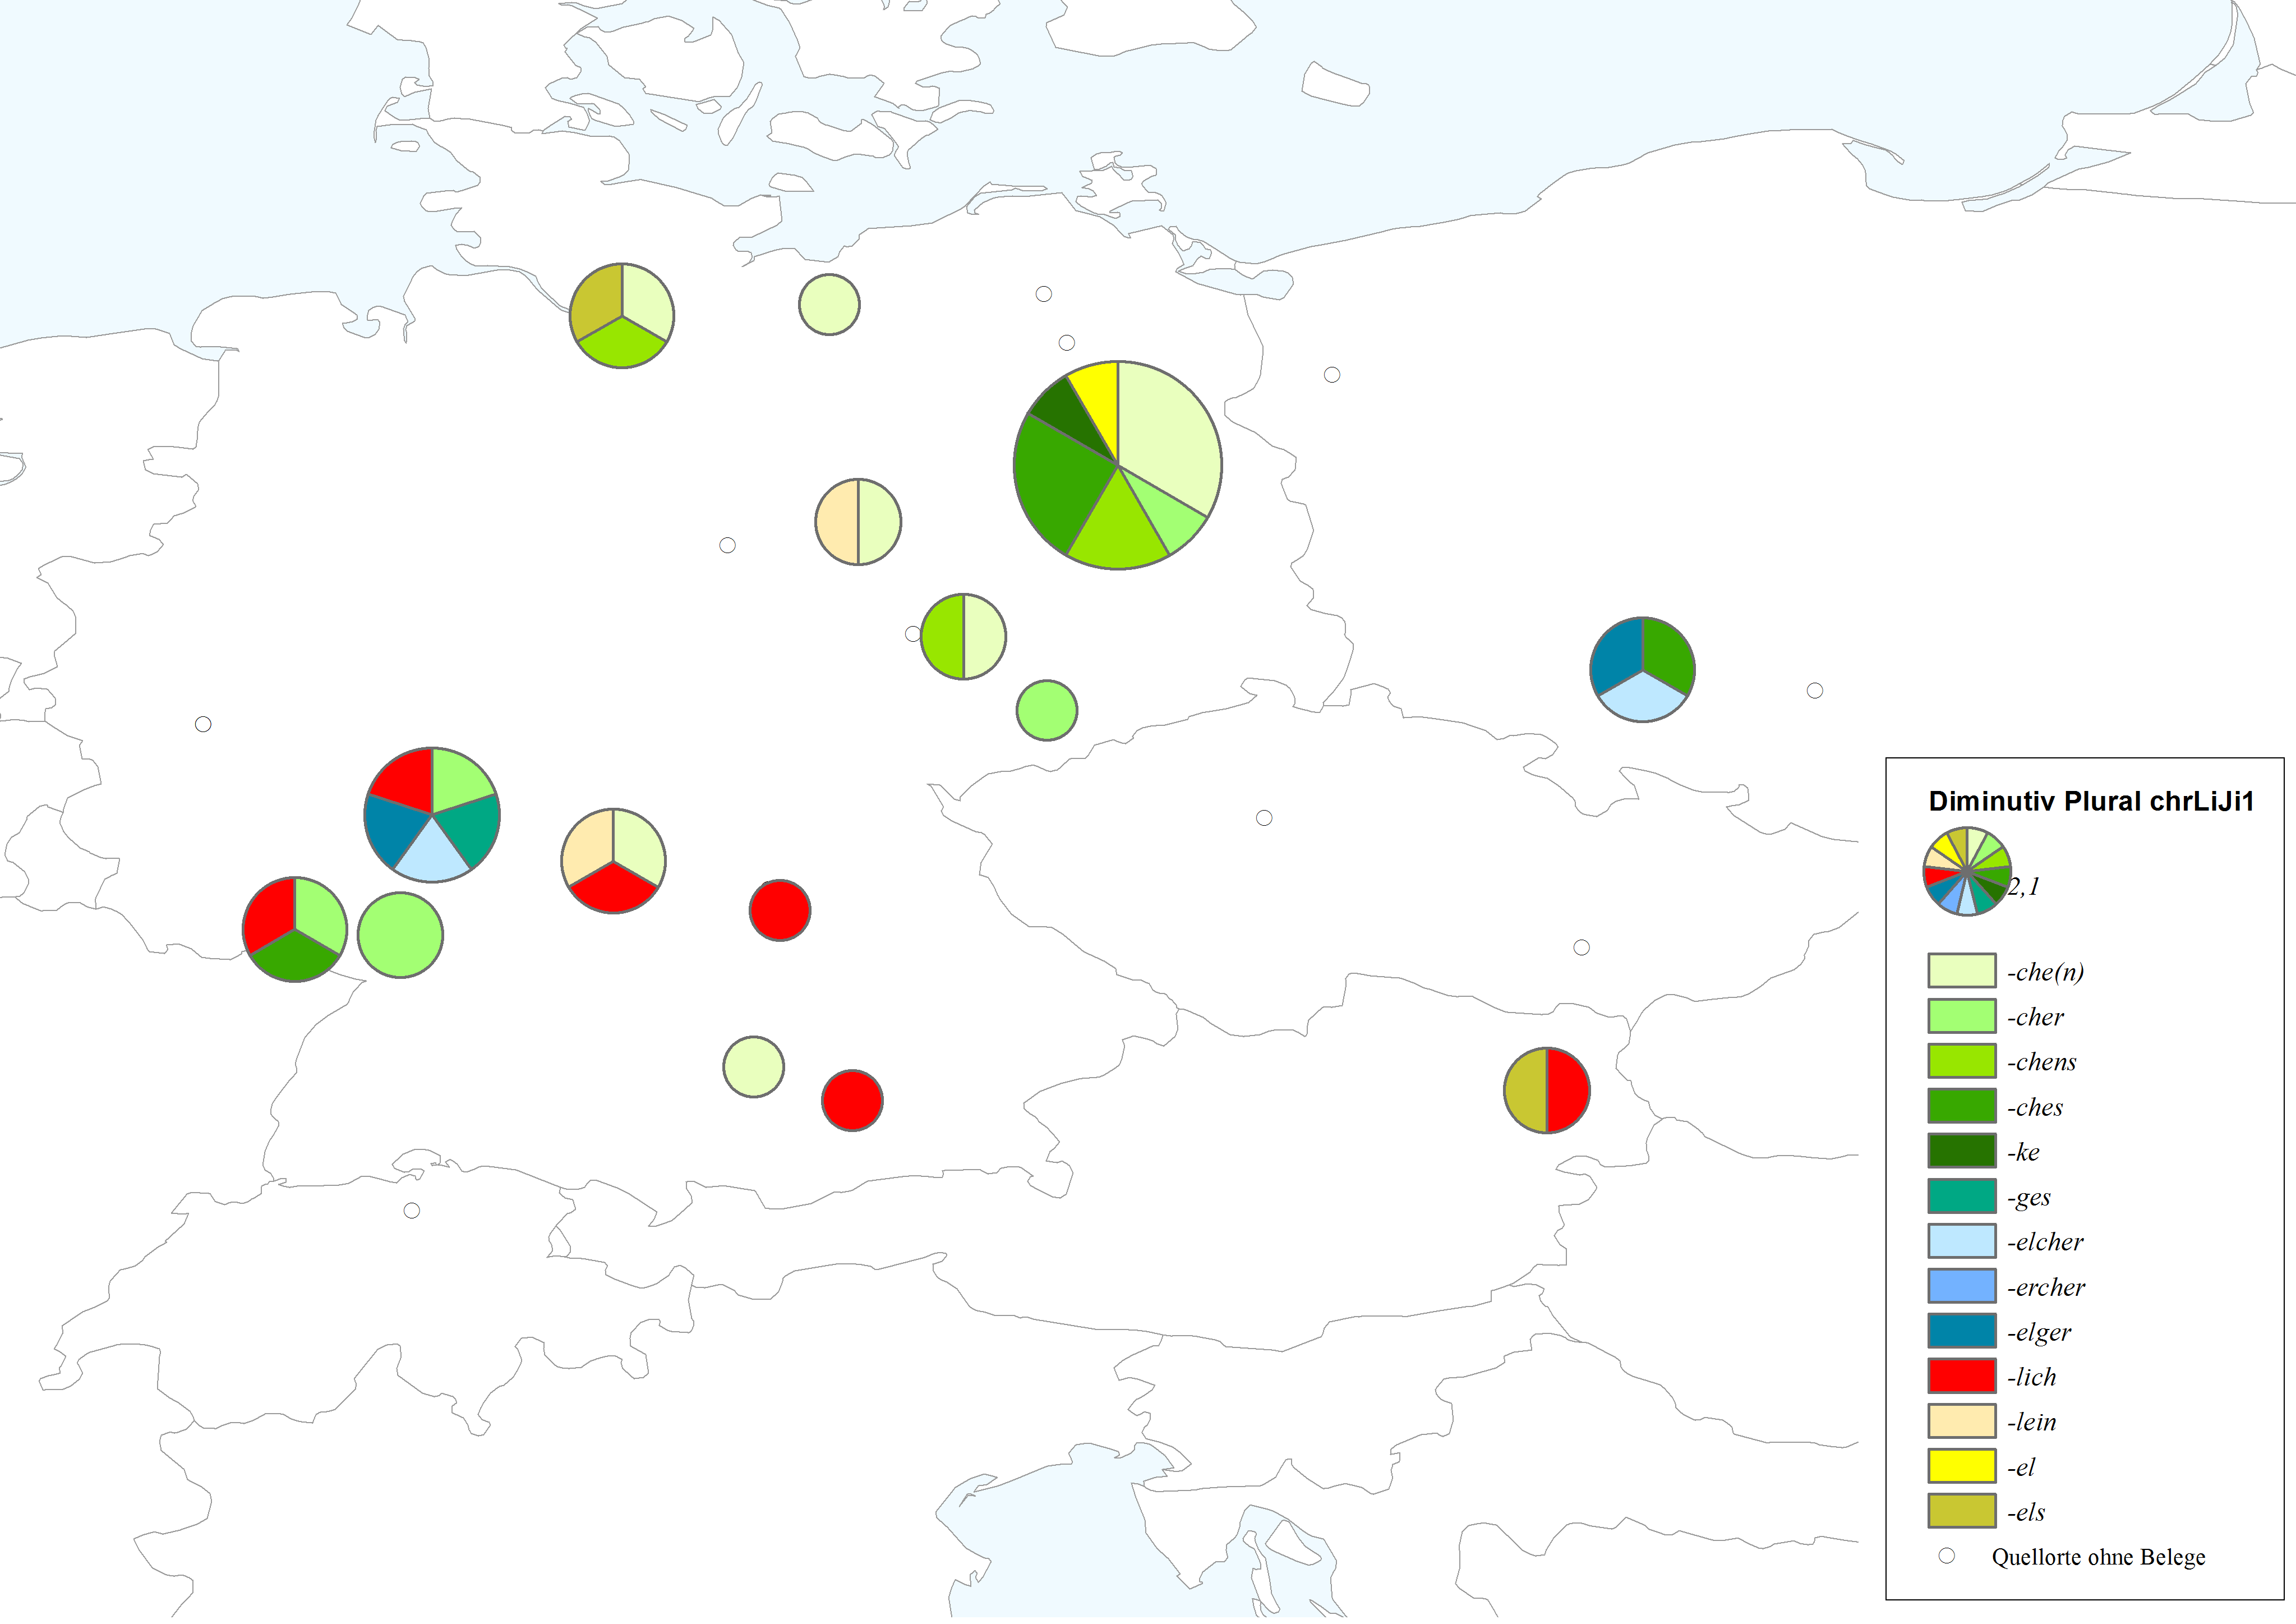
\includegraphics[width=\textwidth]{figures/DIM_PL.png}
		\caption{\label{Dimliji} Pluraldiminutionen im \hai{chrLiJi1} (Einzelsuffixe)}
		\end{figure}  
  
  
  
  \begin{figure} 

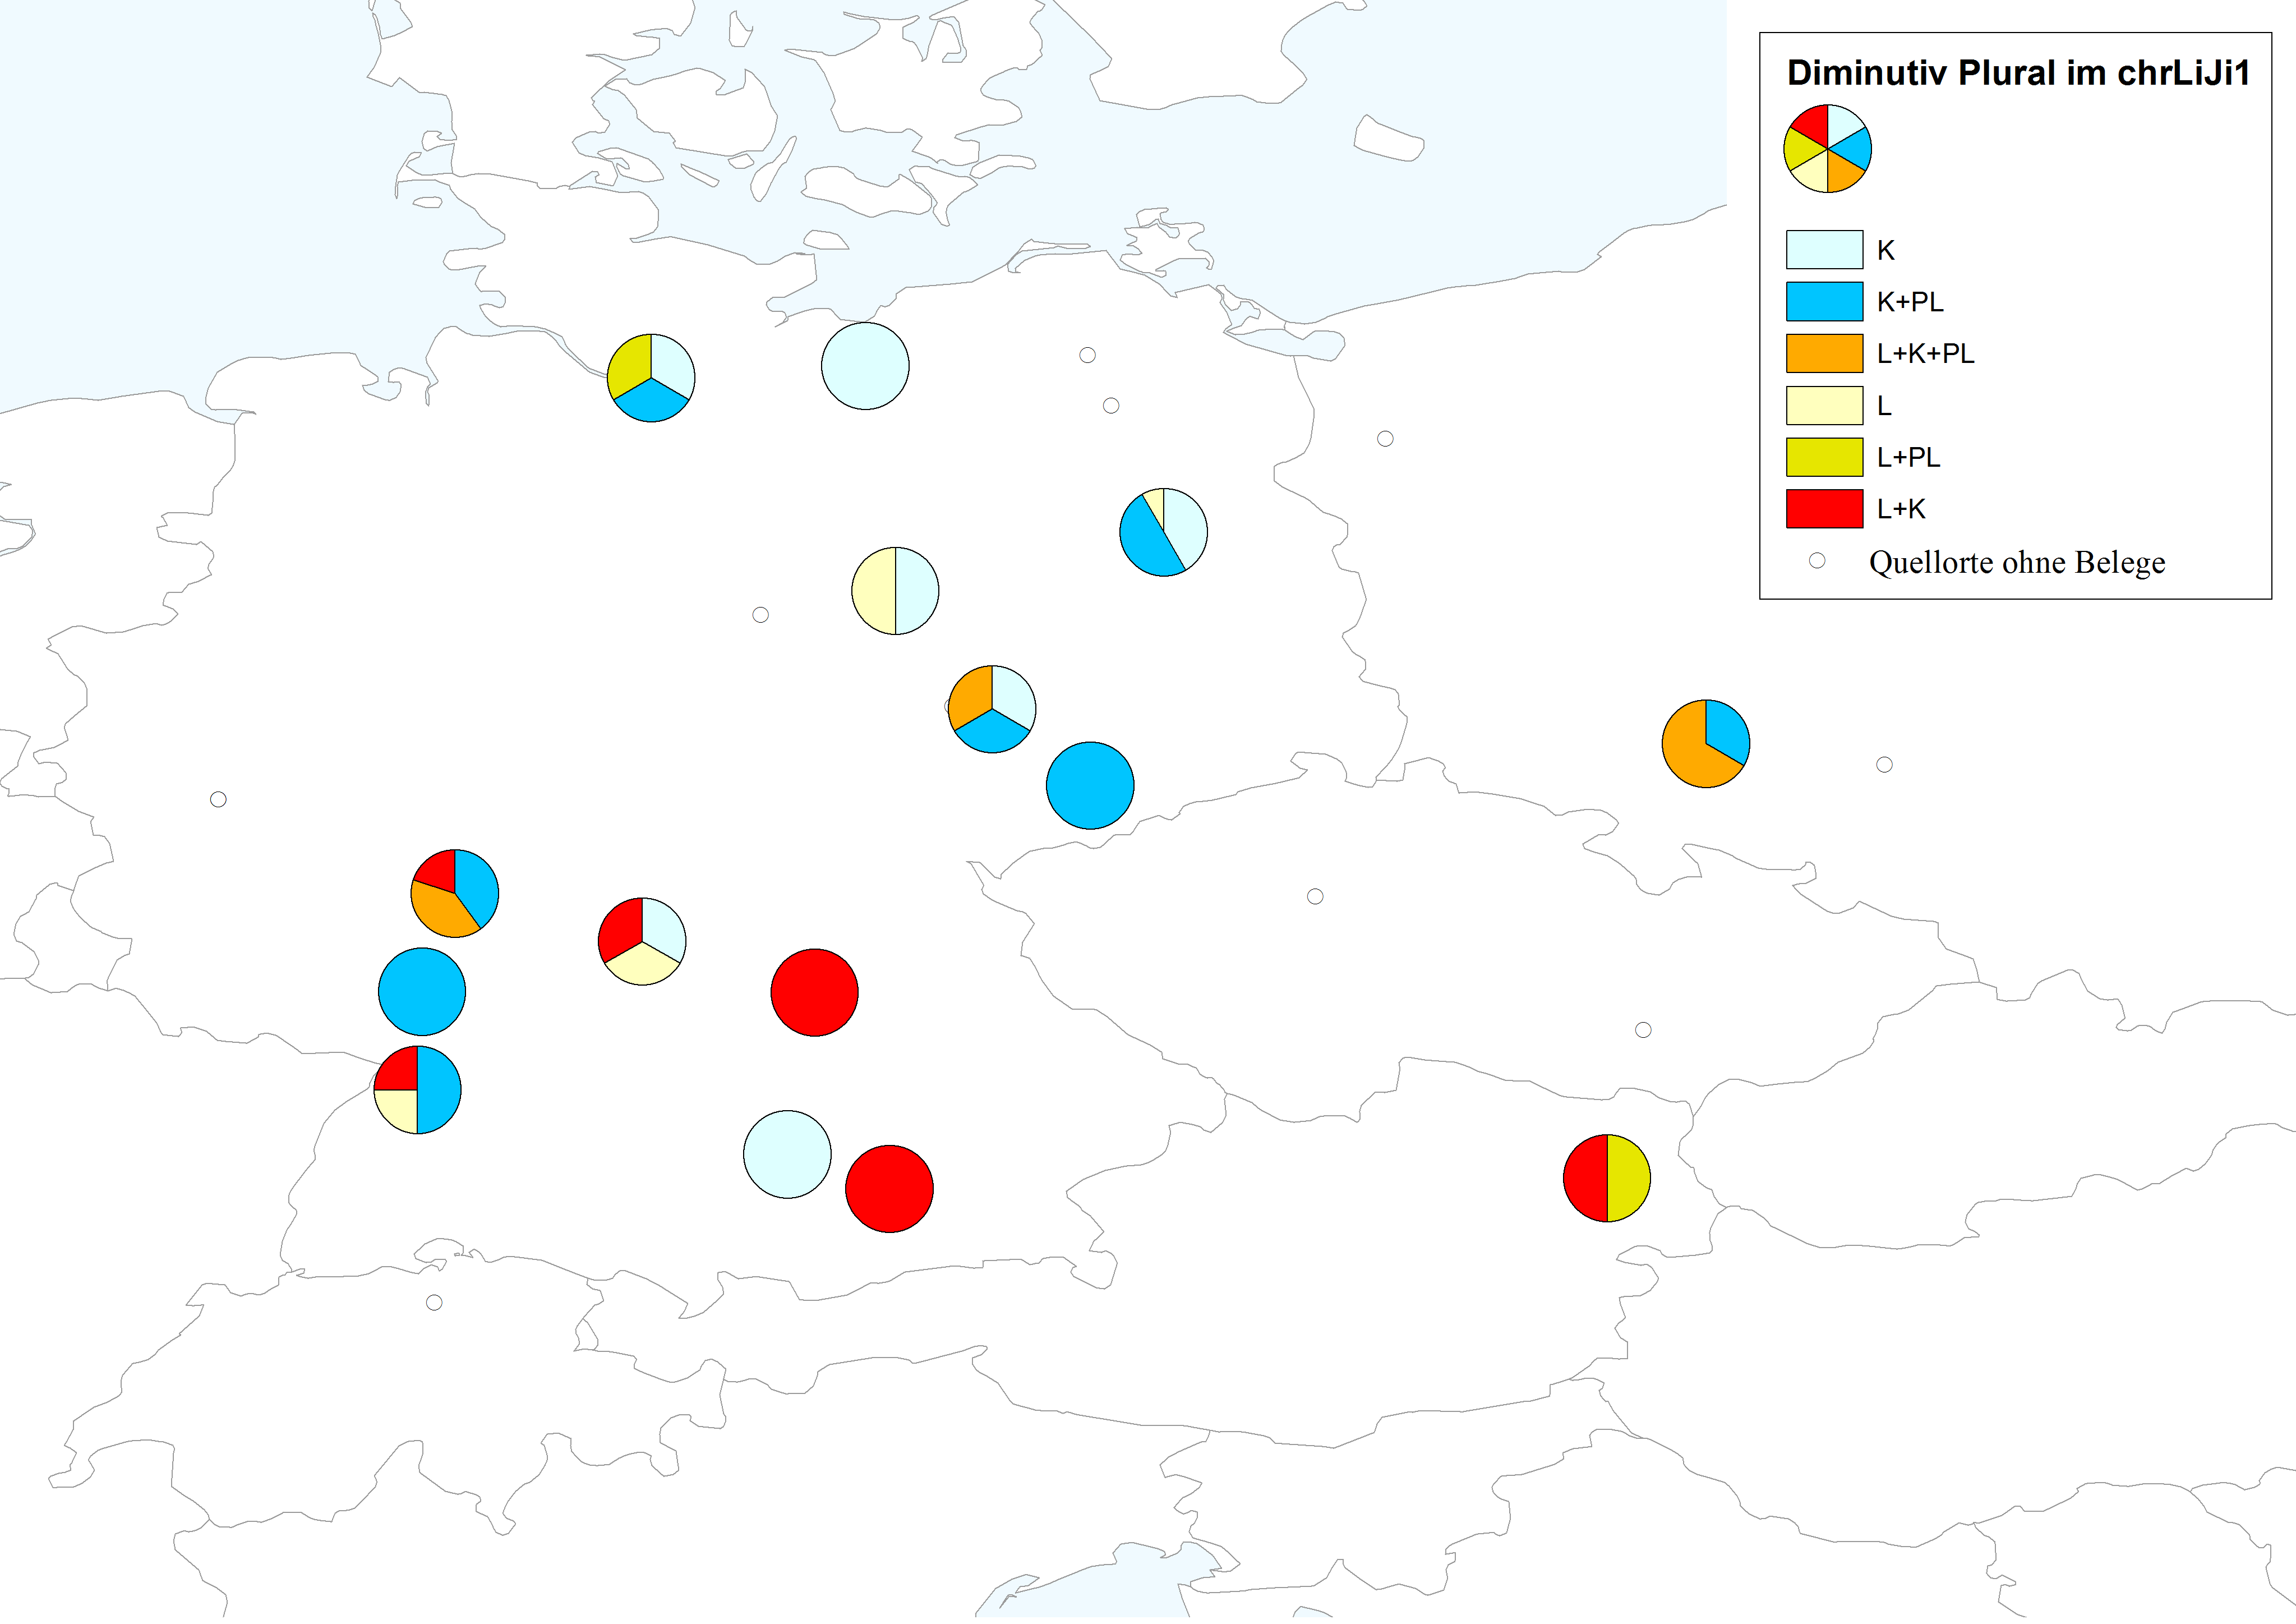
\includegraphics[width=\textwidth]{figures/DIM_PL_kurz.png}
		\caption{\label{Dimlijikurz} Pluraldiminutionen im \hai{chrLiJi1} (Grundmuster)}
		\end{figure}  
  
   
 
 
  
 


  \begin{figure} 

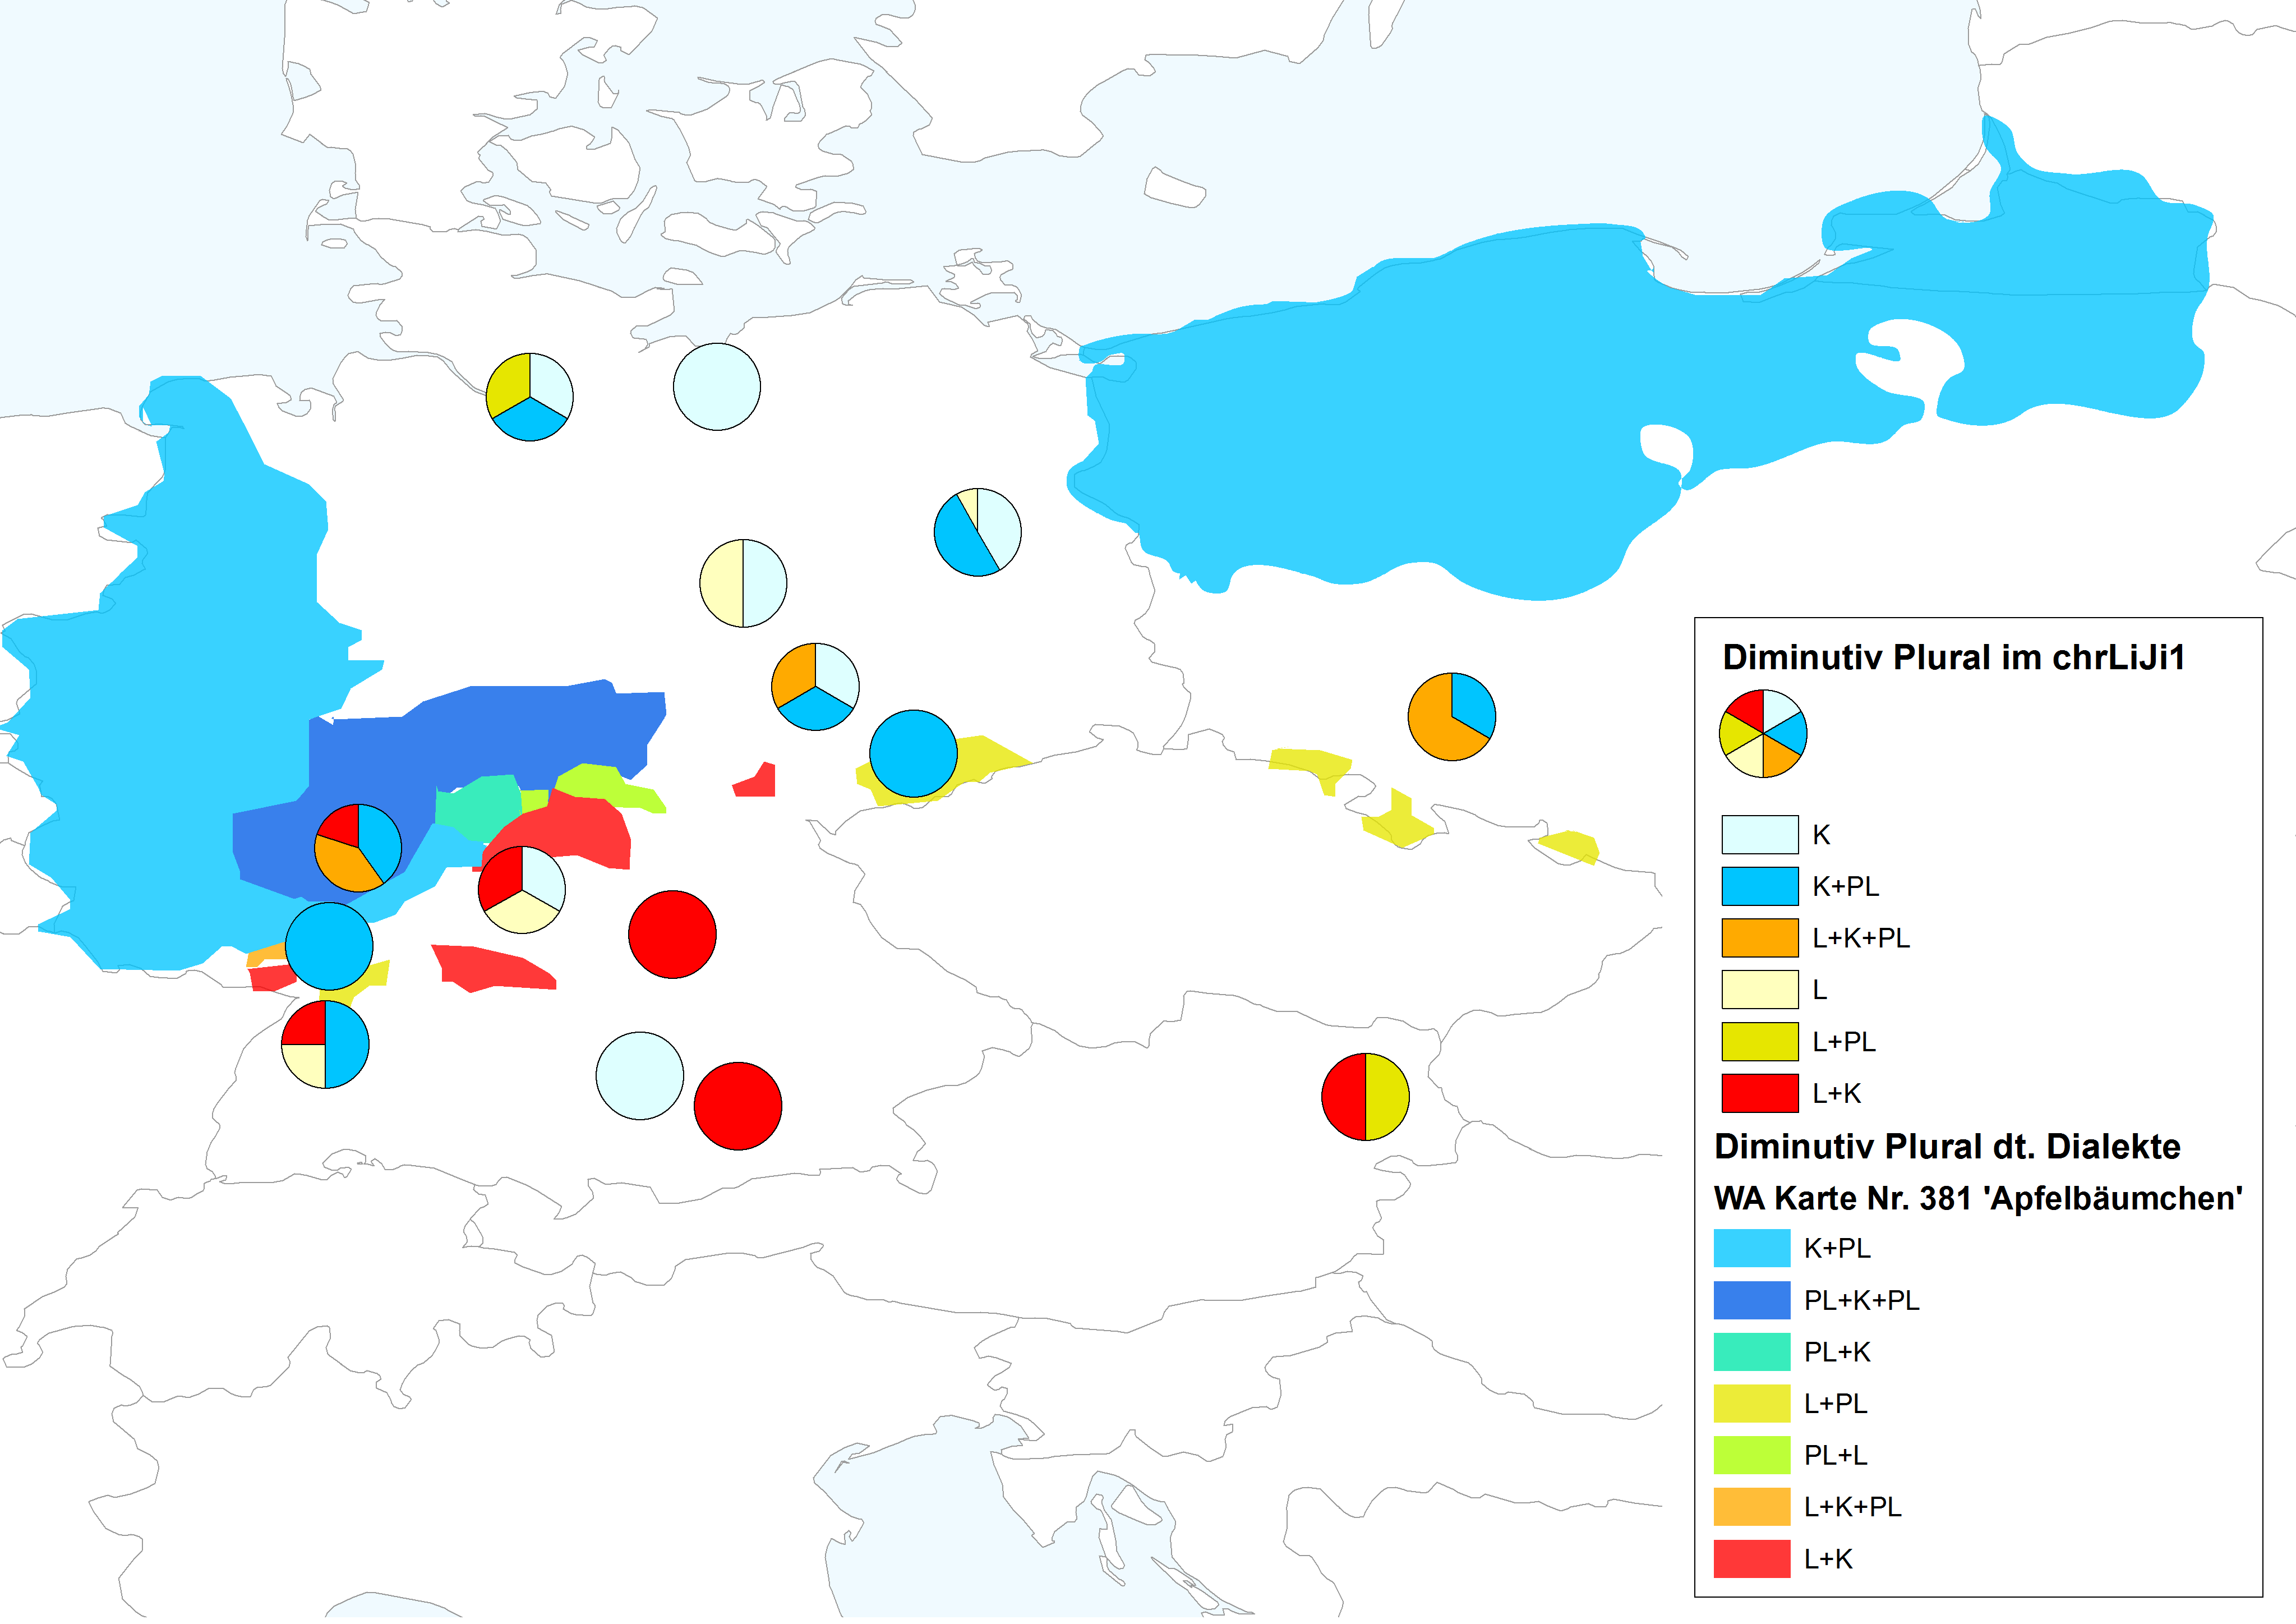
\includegraphics[width=\textwidth]{figures/DIM_PL_DSA_Kurz.png}
		\caption{\label{DimDSALiJi} Pluraldiminutionen im \hai{chrLiJi1} und den dt. Dialekten (\hai{WA} Karte Nr. 381 \sem{Apfelbäumchen})}
		\end{figure}  
 



\begin{figure} 

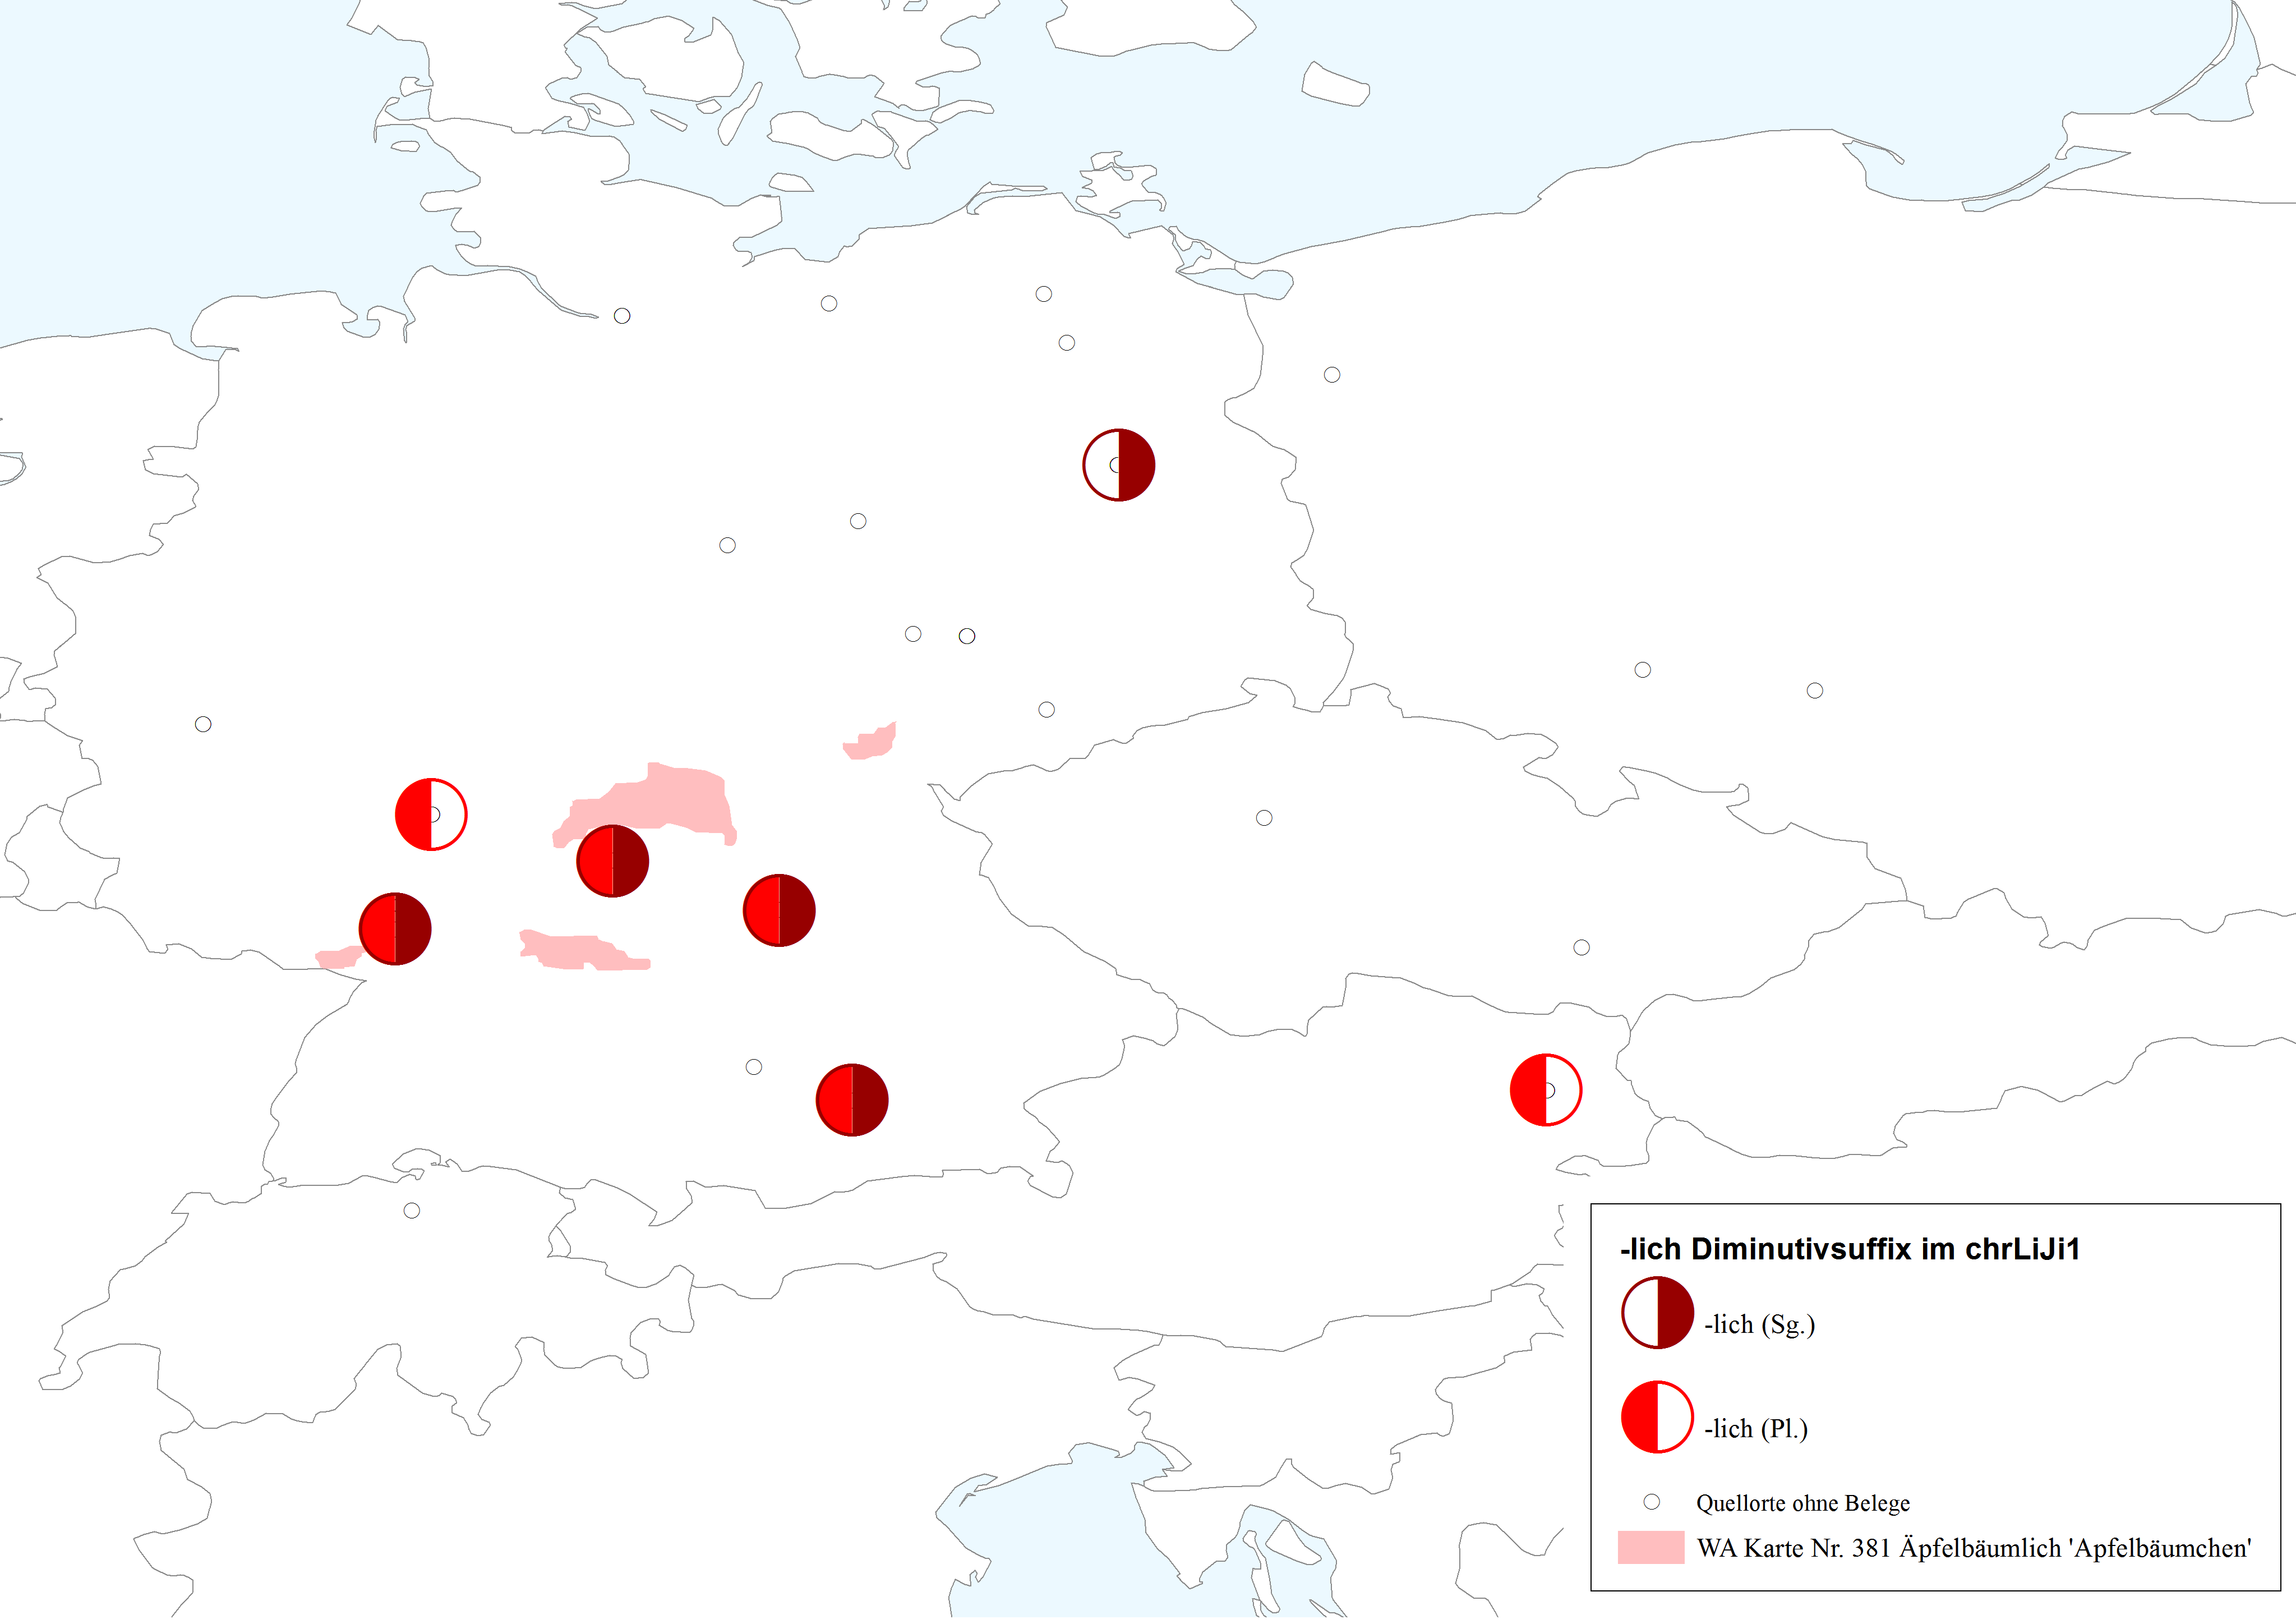
\includegraphics[width=\textwidth]{figures/lich_Dim_pl_sg_DSA.png}
		\caption{\label{DimDSALiJilich} -\textit{lich}-Diminutionen im \hai{chrLiJi1} und den dt. Dialekten (\hai{WA} Karte Nr. 381 \sem{Apfelbäumchen})}
		\end{figure}
  
\newpage 
\subsection{Diminution im \hai{jüdLiJi1} }\label{DIMjüdLiJi1}
%  %\noindent 
Auch im \hai{jüdLiJi1} findet sich eine Vielzahl an Diminutionen. Diese sind in allen der zehn untersuchten Texte belegt. Die Quellen aus Berlin (\hai{GuS1–23}, \hai{PBerlin1–2}) zeigen im Singular wie im Plural allesamt das schriftsprachliche Suffix \textit{-che(n)} (vgl.\, Tabelle \ref{tblDIMjüdliji1SG}). Die südlicheren Quellen verwenden hingegen \hai{L}-Diminutionen. Nur im Fall von \hai{PBreslau} finden sich alle drei Diminutionstypen (\hai{K}, \hai{L}, \hai{L + K}) parallel. 


  \begin{table}
		\begin{tabularx}{\columnwidth}{lXr}
\lsptoprule
\textbf{Suffix} &\textbf{Beispiel} & \textbf{Quellen} \\ \midrule 

\textit{-che(n)} & \textit{Lokomotivche} \sem{Lokomotive\textsubscript{{\Dim} {\Sg}}} (\hai{GuS1}:\,5), \textit{Liedche} \sem{Lied\textsubscript{{\Dim} {\Sg}}} (\hai{GuS5}:\,9), \textit{Geschäftchen} \sem{Geschäft\textsubscript{{\Dim} {\Sg}}}  (\hai{GuS23}:\,12), \textit{Demonschtratziönche} \sem{Demonstration\textsubscript{{\Dim} {\Sg}}} (\hai{PBerlin2}:\, 2.\,Sp.), \textit{Wörtche} \sem{Wort\textsubscript{{\Dim} {\Sg}}} (\hai{PBerlin1}:\,2) & 8 \\ 

 
 \textit{-elche} & \textit{Jüngelche} \sem{Junge\textsubscript{{\Dim} {\Sg}}} (\hai{PBreslau}:\,339) & 1 \\
 
 \textit{-le} & \textit{Schreibebriefle} \sem{Brief\textsubscript{{\Dim} {\Sg}}} (\hai{PAlsleben}:\,Titel, 3) & 1\\

 \textit{-el}/\textit{-l} & \textit{Päckel} \sem{Packet\textsubscript{{\Dim} {\Sg}}} (\hai{PBreslau}:\,342),  \textit{Stückel} \sem{Stück \textsubscript{{\Dim} {\Sg}}} (\hai{PDebrecen}:\,7, 13) & 2 \\
 
 \textit{-ele} & \textit{Büchele} \sem{Buch\textsubscript{{\Dim} {\Sg}}} (\hai{PDebrecen}:\,9),  \textit{Haisele} \sem{Hase \textsubscript{{\Dim} {\Sg}}} (\hai{PDebrecen}:\,13) & 1 \\ 
 
     \lspbottomrule
 \end{tabularx}
		 \caption{Diminutivsuffixe Singular im \hai{jüdLiJi1}}
		 \label{tblDIMjüdliji1SG}
		 \end{table}


  \begin{table}
		\begin{tabularx}{\columnwidth}{lXr}

	\lsptoprule

\textbf{Suffix} &\textbf{Beispiel} & \textbf{Quellen} \\ \midrule 
  \textit{-cher} & \textit{Ameischer} \sem{Ameise\textsubscript{{\Dim} {\Pl}}} (\hai{GuS1}:\,3),  \textit{Perzentcher} \sem{Prozent\textsubscript{{\Dim} {\Pl}}} (\hai{GuS5}:\,7),  \textit{Schwebelhölzcher} \sem{Schwefelholz\textsubscript{{\Dim} {\Pl}}} (\hai{GuS10}:\,5), \textit{Tröppcher} \sem{Tropfen\textsubscript{{\Dim} {\Pl}}} (\hai{PBerlin1}:\,2)  & 4 \\

  \textit{-che(n)} & \textit{Kreppchen} \sem{Krapfen\textsubscript{{\Dim} {\Pl}}} (\hai{GuS15}:\,3), \textit{Bettchen} \sem{Bet\textsubscript{{\Dim} {\Pl}}} (\hai{PBerlin1}:\,2), \textit{Affzierche} \sem{Offizier\textsubscript{{\Dim} {\Pl}}} (\hai{PBerlin2}:\,1.\,Sp.) & 3 \\

 
  \textit{-chers} & \textit{Offißierchers} \sem{Offizier\textsubscript{{\Dim} {\Pl}}} (\hai{PBerlin2}:\,2.\,Sp.) & 1 \\
 
 
  \textit{-ercher} & \textit{Gesetzercher} \sem{Gesetz\textsubscript{{\Dim} {\Pl}}} (\hai{PBerlin1}:\,4) & 1 \\
 
   \textit{-che(n)s} & \textit{Bäckches} \sem{Backe\textsubscript{{\Dim} {\Pl}}} (\hai{PBerlin1}:\,2), \textit{Kupperhütchens} \sem{Kupferhut\textsubscript{{\Dim} {\Pl}}} (\hai{GuS10}:\,10) & 3 \\
   
   \textit{-lech} & \textit{Jidlech} \sem{Jude\textsubscript{{\Dim} {\Pl}}} (\hai{PDebrecen}:\,7),  \textit{Zeitungblättlech} \sem{Zeitungsblatt\textsubscript{{\Dim} {\Pl}}} (\hai{PDebrecen}:\,14)  & 1 \\
  
\lspbottomrule
 \end{tabularx}
		 \caption{Diminutivsuffixe Plural im \hai{jüdLiJi1}}
		 \label{tblDIMjüdliji1PL}
		 \end{table}

 
    
    Besonders authentisch bezüglich der \isi{Diminution} präsentiert sich \hai{PDebrecen}, wo wir den einzigen Beleg einer Pluraldiminution mittels \textit{-lech} finden. Bemerkenswert daran ist, dass wir hier bereits die ostjiddische Vokalisierung des Suffixes antreffen und nicht die westjiddische (\textit{-lich}), wie sie im \hai{chrLiJi1} belegt ist. In den \hai{GuS1–10} finden wir ausschließlich die Pluralsuffixe \textit{-cher} und \textit{-chen} (vgl.\, Tabelle \ref{tblDIMjüdliji1PL}). Eine besondere Vielfalt an Diminutionssuffixen im Plural findet sich in \hai{PBerlin1} (\textit{-chen}, \textit{-ches}, \textit{-ercher}, \textit{-chers}) und \hai{PBerlin2} (\textit{-che}, \textit{-ches}, \textit{-chens}). Diese Suffixe funktionieren nach dem Prinzip \hai{K}+\hai{{\Pl}} (bzw. in einem Fall \hai{{\Pl}}+\hai{K}+\hai{{\Pl}}) und bauen damit auf die \hai{K}-\isi{Diminution} auf. Es findet sich, vom \textit{-lech}-Beleg aus \hai{PDebrecen} abgesehen, kein einziger Beleg für Pluraldiminutiva der Fusionsformen, wie wir sie im \hai{chrLiJi1} besonders im Nordosten finden (vgl.\, S.\, \pageref{LKinberlin}). Hierin besteht also ein deutlicher Unterschied zwischen \hai{chrLiJi1} und \hai{jüdLiJi1}. 

Zusammenfassend lässt sich feststellen, dass im \hai{jüdLiJi1} weniger Aufwand betrieben wurde, Suffixe zu wählen, die nicht der örtlichen deutschen \isi{Diminution} entsprechen, als es im \hai{chrLiJi1} der Fall ist. Das Besondere an den Belegen zur \isi{Diminution} im \hai{jüdLiJi1} ist, dass diese vergleichbar hoch frequent sind wie im \hai{chrLiJi1}. Es ist also vielmehr die reine Präsenz von \isi{Diminution} als deren konkrete morphologische Struktur, die die Gemeinsamkeit beider Formen des \hai{{\LiJieins}} ausmacht. Diminutive können durch die ironische, scherzhafte Funktion des \hai{C2}-Typs provoziert sein und wären damit textsortenspezifisch. Mit Blick auf die Situation im \hai{chrLiJi1} liegt es jedoch nahe, \isi{Diminution} als figurenspezifisch \quein{jüdisch} anzusehen. Darüber hinaus bestärken die Belege aus dem \hai{jüdLiJi1} die Vermutung, dass die Diminutionsmorphologie (insbes. Singulardiminution) im Westjiddischen vielfältig ist und kleinräumige regionale Muster anzunehmen sind. Doch für weitere Ergebnisse dieser Art ist das \isi{Korpus} zum \hai{jüdLiJi1} zu klein und die geographische Streuung der Quellen (auch die aller potenzieller Quellen) zu gering.

 \subsection{Funktionen von Diminution im \hai{{\LiJi}} }\label{DIMFunktionen}
%  %\noindent
   Die Funktion der Diminutivsuffixe im \hai{chrLiJi1} ist schwer auszumachen. Zum einen ist es möglich, dass mit ihnen  eine tatsächliche Sprachrealität abgebildet wird, die aufgrund der dünnen Quellenlage nicht klar umrissen werden kann, zum anderen aber sind die Formen areal und diachron zu wahllos verbreitet, als dass dies Rückschlüsse auf feinere Strukturen zuließe. Was grobe Raumstrukturen betrifft, so bieten die Daten des \hai{chrLiJi1} immerhin Ansätze für weitere Untersuchungen. Durch authentische Quellen zu prüfen wären besonders die Hypothesen, dass \hai{L+K}-Fusionsformen im Singular im Nordosten des Westjiddischen verbreitet waren oder dass die Pluraldiminution mittels -\textit{lich} lediglich im Süden des Sprachgebiets tatsächlich verwendet wurde, während im Norden andere, auf \hai{K}-Diminutionen aufbauende Formen, präsent waren.


Die Analyse hat gezeigt, dass sich die Quellen des \hai{jüdLiJi1}  ähnlich den koterritorialen Quellen des \hai{chrLiJi1} verhalten. Andererseits irritiert besonders, dass wir im \hai{chrLiJi1} eine solch große Variation an Suffixen vorfinden, die uns aus den jiddischen Varietäten nicht bekannt ist (vgl.\, Abschnitt \ref{dimJIDDISCH}) und auch nicht durch Daten des \hai{jüdLiJi1} bestätigt wird. Hinzu kommt, dass sich \isi{Diminution} außerhalb des \hai{{\LiJi}} als Charakteristikum der jiddischen Sprache etabliert haben muss, anders ist nicht zu erklären, warum sie bereits vielfach in den frühesten Quellen belegt ist (vgl.\, Abbildung \ref{REGDIMSG}). Dies spricht dafür, anzunehmen, dass \isi{Diminution} an sich, also unabhängig der morphologischen Struktur des Suffixes, besonders stark als grammatische Kennfunktion \textit{jüdischer Sprache} agiert. Um ein besseres Bild der Funktionen von \isi{Diminution} im \hai{{\LiJi}} zu gewinnen, bedarf es allerdings weiterer Daten der gesprochenen und geschriebenen Sprache. Erst dann könnte geklärt werden, ob ein äußerst hoher Gebrauch an Diminutiva tatsächlich der jiddischen Sprachrealität entspricht oder nicht. 

 \section{Plurale}\label{pl}
 %\noindent

\largerpage[-1]
In einigen Fällen weist das \hai{{\LiJi}} Pluralformen auf, die vom Schriftdeutschen abweichen. Besonders populär ist dabei die Verwendung des  \textit{s}-Plurals (vgl.\, Unterabschnitte S.\, \pageref{sPlural} u. S.\, \pageref{sPluralLiJi}). Eine weitere, jedoch deutlich seltener auftretende Pluralmorphemalternanz wird in Unterabschnitt \ref{erPLURAL} vorgestellt. Bevor auf die Daten zum \hai{{\LiJi}} näher eingegangen wird, gibt der nachfolgende Unterabschnitt \ref{plDEUJI} einen allgemeinen Überblick zu den Grundmustern der Pluralbildung im Jiddischen und Deutschen.


 
\subsection{Grundmuster der Pluralmorphologie im Jiddischen und Deutschen}\label{plDEUJI}
%  %\noindent 
 Das Pluralsystem
%  in den deutschen Dialekten 
der deutschen Dialekte ist alles andere als einheitlich. Nicht nur, dass dialektale Variation bei der Wahl der Pluralisierungsstrategie vorliegt, sondern es gibt  in den Dialekten  Strategien, wie z.\,B.\, Pluralmarkierung durch \isi{Subtraktion} (vgl.\, \citealt{GolstonWiese1996,HolsingerHouseman1999,Knaus2003,BirkenesDiss}), die die Schriftsprache nicht kennt (vgl.\, \citealt[414–443]{Schirmunski1962}; \citealt{Nuebling2005}; \citealt[insbes. 155–169]{Wiese2009}). Pluralisierung im Jiddischen folgt in den meisten Fällen Strategien, die auf die germanische Komponente zurückgehen. Der Plural wird überwiegend nach den folgenden Prinzipien gebildet: -\textit{er}, -\textit{(e)n}, -\textit{∅},  -\textit{(e)s},\footnote{Ob sich die Existenz eines \textit{s}-Plurals im Jiddischen auf die alt- bzw. mittelhochdeutsche Komponente zurückführen lässt, ist anzweifelbar (vgl.\, etwa \citealt{King1990,Timm2007}). Da dies eine Strategie ist, die germanischen Sprachen an sich nicht fremd ist. Denn selbst wenn der \textit{s}-Plural im Jiddischen nicht genuin deutschen Ursprungs ist, so wird das germanische Grundgerüst des Jiddischen, welches einen alt-/\,mittelhochdeutschen Ur\-sprung hat, die Aufnahme dieses Plurals begünstigt und katalysiert haben. Weiter ist zu sagen, dass der einfache -\textit{e}-Plural ± \isi{Umlaut} im Jiddischen durch die \isi{Apokope} abgebaut wurde (\citealt[29]{Timm2007}).\label{FNsplural}} ± \isi{Umlaut} (\ref{PLji1erUmlaut}–\ref{PLji1nurUmlaut} zitiert n. \citealt[163]{Jacobs2005}). Hinzu kommt die aus der \ili{hebräisch}-aramäischen Komponente stammende Pluralbildung mittels  -\textit{im}/ -\textit{em}, die überwiegend auf Lexeme dieser Komponente angewendet wird (\ref{PLji1Hebr} zitiert n. \citealt[165]{Jacobs2005}) und nur in wenigen Ausnahmefällen Lexeme anderer Komponenten betrifft (\ref{PLji1Hebrgerm} zitiert n. \citealt[165]{Jacobs2005}). 
 Wie bereits gezeigt, verfügt das Jiddische über eine gesonderte Pluralbildung im Rahmen der \isi{Diminution} (vgl.\, Abschnitt \ref{dim}).

Wie in den deutschen Dialekten, so gibt es auch in den jiddischen Dialekten areale Variation (\ref{PLji1dialekt}). Zur Situation in den westjiddischen Dialekten fehlt es noch an Detailanalysen, es ist aber anzunehmen,  dass dort ebenso wie in den deutschen und ostjiddischen Dialekten diatopische Variation zu erwarten ist, welche u.\,U. sogar parallel zu denen der deutschen Dialekte liegt. So finden wir etwa in einer unserer ältesten Quellen des gesprochenen Westjiddischen, der \qu{Hochzeit zu Grobsdorf}, bereits  Belege für Interferenzen mit den örtlichen hessischen Dialekten, wo der \textit{-er}-Plural besonders \isi{produktiv} ist (s. \ref{PLWJgrob};vgl.\, \citealt[83]{Friebertshaeuser1987}). %rs + "s. Bsp. "

\newpage 

 \eenumsentence{
 \item {\Sg} \RL{לא\makebox(-1.5,-7.5)[r]{\libertineGlyph{uni207B}}נד} \textit{land} \sem{Land} – {\Pl} \RL{לענדער} \textit{lender} \sem{Länder} \label{PLji1erUmlaut} 
 \item {\Sg} \RL{וו{יי}\makebox(-1.5,-3.5)[r]{\libertineGlyph{uni207B}}ב} \textit{vayb} \sem{Weib, Frau} – {\Pl} \RL{וו{יי}\makebox(-1.5,-7.5)[r]{\libertineGlyph{uni207B}}בער} \textit{vayber} \sem{Weiber, Frauen} \label{PLji1nurer}
 \item {\Sg} \RL{ט{יי}\makebox(-1.5,-3.5)[r]{\libertineGlyph{uni207B}}ך} \textit{taykh} \sem{Fluss} – {\Pl} \RL{ט{יי}\makebox(-1.5,-7.5)[r]{\libertineGlyph{uni207B}}כן} \textit{taykhn} \sem{Flüsse} \label{PLji1n} 
  \item {\Sg} \RL{זינגער} \textit{zinger} \sem{Sänger} – {\Pl} \RL{זינגערס} \textit{zingers} \sem{Sänger} \label{PLji1s} 
 \item {\Sg} \RL{הא\makebox(-1.5,-7.5)[r]{\libertineGlyph{uni207B}}נט} \textit{hant} \sem{Hand} – {\Pl} \RL{הענט} \textit{hent} \sem{Hände} \label{PLji1nurUmlaut}
 \item {\Sg} \RL{למדן} \textit{lamdn} \sem{Gelehrter} – {\Pl} \RL{למדים} \textit{lomdem} \sem{Gelehrte} \label{PLji1Hebr}  
  \item {\Sg} \RL{ד{א\makebox(-1.25,-1.25)[r]{\libertineGlyph{uni05B8}}}קטער} \textit{dokter} \sem{Arzt} – {\Pl} \RL{ד{א\makebox(-1.25,-1.25)[r]{\libertineGlyph{uni05B8}}}קטוירים} \textit{doktoyrim} \sem{Ärzte} \label{PLji1Hebrgerm} 
 \item Standard {\oj} u. \hai{{\NOJ}}: {\Sg} \RL{נ{א\makebox(-1.25,-1.25)[r]{\libertineGlyph{uni05B8}}}ז} \textit{noz} \sem{Nase} – {\Pl}  \RL{נעזער} \textit{nezer};\\
 \hai{{\ZOJ}}: {\Sg} \RL{נ{א\makebox(-1.25,-1.25)[r]{\libertineGlyph{uni05B8}}}ז} \textit{noz} \sem{Nase} –  {\Pl} \RL{נייז} \textit{neyz};\\
 \hai{{\SÜJ}} {\Sg} \RL{נ{א\makebox(-1.25,-1.25)[r]{\libertineGlyph{uni05B8}}}ז} \textit{noz} \sem{Nase} –  {\Pl} \RL{נ{א\makebox(-1.25,-1.25)[r]{\libertineGlyph{uni05B8}}}זן} \textit{nozn} \sem{Nasen}\\
 (Bsp. zitiert n. \citealt{Weinreich1960b};\citeyear[9–11]{Weinreich1962})\label{PLji1dialekt} 
    \item {\Sg} \RL{סלו{פ\makebox(-1,4)[r]{\libertineGlyph{afii57807}}}} \textit{slup} \sem{Pfahl} – {\Pl} \RL{סלו{פ\makebox(-1,4)[r]{\libertineGlyph{afii57807}}}ס} \textit{slups} \sem{Pfähle} \label{PLji1sslav} 
    \item {\Pl} \RL{מענשער} \textit{mensher} \sem{Menschen} (\qu{Die Hochzeit zu Grobsdorf} 1822:\,33) \label{PLWJgrob}    
 }
 
 
 %\subsection{Der \textit{s}-Plural im Jiddischen und Deutschen} %ls zusammengefasst mit vorangegangener subsection
 
 %  %\noindent
 Ein besonders umstrittenes Thema in der Germanistik und Jiddistik ist die Genealogie des \textit{s}-Plurals (vgl.\, Fn. \ref{FNsplural}).\label{sPlural} Die Pluralbildung mittels der Suffigierung des Konsonanten \textit{s} ist in vielen modernen romanischen und germanischen Sprachen zu finden. Neben Deutsch und Jiddisch haben z.\,B.\, Französisch, Spanisch, Portugiesisch, Englisch, Niederländisch (und die niederdt. Dialekte), Afrikaans, (West-)Friesisch und  festlandskandinavische Sprachen ein \isi{Pluralsuffix} \textit{-s}; hingegen nicht zu finden \,%rs - ","
 ist es im Isländischen, Färöischen, Italienischen oder Rumänischen\footnote{Im Lateinischen gibt es allerdings Plurale auf -s.} (vgl.\, \citealt{NueblingSchmuck2010}; \citealt[88]{Hoekstra2001}). Obwohl dieser Konsonant damit als Pluralmarker im \quein{Europäischen Sprachbund} sehr weit verbreitet ist, unterscheiden sich die einzelnen Sprachen 
deutlich sowohl im synchronen Gebrauch als auch in den diachronen Entwicklungen zu stark voneinander, als dass ein gemeinsamer Ursprung klar erkennbar wäre. Generell sind Plurale auf \textit{-s} ein eher junges Phänomen der romanischen und germanischen Sprachen und es tritt in den meisten Sprachen zwischen dem 9. und 15. Jahrhundert erstmals in Erscheinung (vgl.\, \citealt{NueblingSchmuck2010}). Es ist gut möglich, dass die \textit{s}-Plurale in den europäischen Sprachen unabhängig voneinander durch internen Sprachwandel entstanden sind und dieser Konsonant aus phonologischen Gründen in diesen Sprachen eine leichte Strategie zur Pluralbildung problematischer Lexeme und untypischer phonologischer Strukturen (wie sie vorwiegend in Fremdwörtern zu finden sind) darstellt (vgl.\, \citealt{Wiese2009}).
 
  
 In den festlandgermanischen Sprachen tritt ein \textit{s}-Plural erstmals im Mittelniederländischen auf (\citealt{NueblingSchmuck2010}; \citealt[422–425]{Schirmunski1962}). Seine Herkunft ist stark umstritten. Manch einer nimmt einen romanischen (altfranzösischen) Einfluss an; andere wiederum sehen den altsächsischen (bzw. altenglischen) \textit{os}/\textit{as}-Plural als Vorbild an (vgl.\, \citealt{Philippa1981, Philippa1982,Oehmann1924}). \,%rs großbuchstabe
 Gegen den französischen Einfluss spricht besonders, dass zum Zeitpunkt des erstmaligen Aufkommens von \textit{s}-Pluralen im Niederländischen (frühes 13. Jahrhundert) dieser im Altfranzösischen selbst noch gar nicht ausgebildet war und nur für Maskulina im \isi{Akkusativ} Plural galt (\citealt[150]{NueblingSchmuck2010}). Und auch ein altsächsischer Einfluss wäre äußerst ungewöhnlich und ist auch besonders problematisch, da eine Überlieferungslücke von \textit{os}/\textit{as}- bzw. \textit{s}-Plural zwischen dem frühen 12. und dem 13. Jahrhundert vorliegt (\citealt[151]{NueblingSchmuck2010}).

 
Während der  \textit{s}-Plural im Niederländischen und Niederdeutschen äußerst \isi{produktiv} wird, ist er für das Hochdeutsche kaum belegt. Erst im Mittelhochdeutschen ist er erstmals bezeugt. Ein französischer Einfluss ist hier weitgehend auszuschließen, u.\,a.\, da er bei französischen Entlehnungen nicht belegt ist und auch nicht besonders frequent in Dialekten entlang der deutsch–\ili{französisch} Sprachgrenze ist, sondern im Gegenteil der \textit{s}-Plural dort kaum üblich ist (\citealt[122–126]{Oehmann1924}). Eine Genese des Mittelhochdeutschen \textit{s}-Plurals aus dem Niederdeutschen ist problematisch, da dieser zwar im Altniederdeutschen noch belegt ist, für das Mittelniederdeutsche, also der Kontaktsprache zum Mittelhochdeutschen, aber nicht bezeugt ist, in den modernen niederdeutschen Dialekten aber hingegen wieder äußerst \isi{produktiv} ist (\citealt[147–150]{Lindowetal1998}). Auch im Frühneuhochdeutschen ist der \textit{s}-Plural noch äußerst selten belegt. Ab 1700 steigen die Belegzahlen besonders bei Lehn- und Fremdwörtern langsam an; in autochthon deutschen Lexemen ist er aber nach wie vor, besonders im niederdeutschen und nördlichen westmitteldeutschen Raum, \,%rs + ,…,
verbreitet (\citealt[266]{Wegera1987}). \,%rs Zitierbefehl fehlte
Ein überzeugendes Szenario für die Herleitung des \textit{s}-Plurals im Gegenwartsdeutsch geht davon aus, dass der \textit{s}-Plural auf das Genitiv-\textit{s} bei \isi{Eigennamen} (insbes. Familiennamen) zurückgeht (\citealt[93]{Wegener2004}; \citealt{NueblingSchmuck2010};vgl.\, \citealt[436f]{Schirmunski1962}).
   
Im gegenwärtigen Hochdeutschen finden wir den \textit{s}-Plural besonders bei Neutra (4,7\% Tokens), selten bei Maskulina (1,4\% Tokens) und äußerst selten bei Feminina (0,2\% Tokens) (\citealt[45–48]{Pavlov1995}). Deutlich häufiger sind Lehn- und Fremdwörter von der Pluralisierung mittels \textit{s} betroffen. \citealt{Wegener2004} zeigt, dass der \textit{s}-Plural hier oft als \quein{Übergangssuffix} fungiert und ein Lexem oft die Deklinationsklasse wechselt sobald es grammatisch integriert ist  (\textit{Pizzas} > \textit{Pizzen}, \textit{Kontos} > \textit{Konten}). Dies ist aber keine Regel und viele Fremdwörter, insbes. gekürzte Fremdwörter, behalten den \textit{s}-Plural (\textit{Autos} > *\textit{Auten}, \textit{Limos} > *\textit{Limen}).
   
 Im modernen Jiddischen ist der \textit{s}-Plural deutlich frequenter als im Deutschen (\citealt{Timm2007}). Er wird z.\,B.\, auf fast alle Maskulina auf -\textit{er}, alle Feminina auf -\textit{in}, viele zweisilbigen Wörter auf -\textit{n}, den überwiegenden Teil aller Substantive der slawischen Komponente (\ref{PLji1sslav} zitiert n. \citealt[163]{Jacobs2005}) und alle auf Vokal ausgehenden Lehnwörter angewandt (\citealt{Timm2007}). Für die diachrone Entwicklung zeigt \cite{Timm2007} drei in (\ref{sPluraljiddischTIMM}) zusammengefasste Phasen auf, 
 in denen sich der \textit{s}-Plural im Jiddischen mehr und mehr ausbreitet. Während \cite[28, 115]{Bin-Nun1973} und \cite{Timm2007} für einen romanischen (Loez) Ursprung des jiddischen \textit{s}-Plurals plädieren (vgl.\, \citealt{Neuberg2007}), sprechen sich \cite[37]{Birnbaum1922}, \cite{King1990}, \cite[399]{Krogh2001} und \cite[402]{Jacobsetal2013} für eine hebräische Genese aus dem Plural für Feminina \RL{ות}- \textit{-ot} und der aschkenasischen Frikativierung von {\hebr} \RL{ת} \textit{t} zu \textit{s} aus. Nur \cite[63–68]{Weinreich1973} verbindet beide Hypothesen und meint, dass sowohl Alt\ili{französisch} als auch Hebräisch dazu beigetragen haben, im Jiddischen den \textit{s}-Plural zu begünstigen. Prinzipiell können alle Argumente, die gegen einen romanischen Ursprung der hoch- und niederdeutschen \textit{s}-Plurale sprechen, auch auf das Jiddische angewandt werden. 
 
  \eenumsentence{
 \item [] \textbf{Phase 1 (11. Jh. – ca.\, 1435):} \textit{s}-Plural in ca.\, 50 Lexemen bezeugt; nicht auf bestimmte Deklinationstypen begrenzt.
 \item [] \textbf{Phase 2 (von 1435–1580):} Zwei Drittel der Belege sind Feminina auf {\mhd} -\textit{in(ne)}. Das restliche Drittel sind Fremd-, Lehnwörter u. Internationalismen.
\item [] \textbf{Phase 3 (seit 1580):} Der \textit{s}-Plural macht die Hälfte aller Pluralbelege aus.
 } \label{sPluraljiddischTIMM}
 

 Der Unterschied zwischen Jiddisch und Deutsch liegt damit nicht nur in der unterschiedlich starken Verwendung des \textit{s}-Plurals, sondern auch in der unterschiedlichen historischen Entwicklung 
dieses Plurals. 
Besonders auffällig ist, dass das Jiddische wesentlich früher als Deutsch einen \textit{s}-Plural etabliert. Mit Blick auf die Stadien \citeauthor{Timm2007}s (\citeyear{Timm2007};
 s. \ref{sPluraljiddischTIMM}) fällt auf, dass besonders während der frühneuhochdeutschen Zeit (1350–1545) der \textit{s}-Plural im Jiddischen einen Zuwachs erfahren hat und systematisiert wurde. In dieser Zeit fanden entscheidende Entwicklung im Jiddischen statt, die es vom Deutschen und seinen Varietäten deutlich entfernte (\citealt{Timm2005,Santorini1992, Santorini1993b, Santorini1993a}). Es ist damit m.\,E. ein durchaus plausibles Szenario, anzunehmen, dass der Unterschied bezüglich der Verwendung und \isi{Frequenz} des \textit{s}-Plurals zwischen 
% modernem 
dem modernen
Deutsch und
%  modernem
dem modernen Jiddisch mit der starken Auseinanderentwicklung beider Varietäten in früh-frühneuhochdeutscher Zeit erklärbar ist (\citealt{Timm2005}). Ein gemeinsamer Ursprung des \textit{s}-Plurals – ggf. im Jiddischen durch den hebräischen Plural zusätzlich begünstigt – wäre damit anzunehmen. Dafür spricht besonders, dass in beiden Sprachen Fremd- und Lehnwörter mittels \textit{s} pluralisiert werden. Die hohe \isi{Frequenz} an \textit{s}-Pluralen bei Nomen der slawischen Komponente spräche für eine funktionale Nähe zum Deutschen, wo dies eine übliche Pluralbildung für Lehn- und Fremdwörter ist (s.\,o.; vgl.\, \citealt{Wegener2004}). 
 
 
 
  \subsection{Der \textit{s}-Plural im Literaturjiddischen}\label{sPluralLiJi}
  %  %\noindent  
  19 Quellen des \hai{chrLiJi1} verwenden einen \textit{s}-Plural, wo er im Schriftdeutschen unüblich ist. Er findet sich im \hai{chrLiJi1} in allen Genera und auch eine Präferenz bestimmter Kasus ist nicht zu erkennen. Eine Quelle (\hai{NW} Berlin, 1804) zeigt ihn in fünf unterschiedlichen Kontexten (\isi{Gallizismus}, \isi{Hebraismus}, \textschwa-Plural, ∅-Plural, \isi{Diminution}); sechs Quellen verwenden das Plural\textit{-s} in je zwei unterschiedlichen Kontexten. Das Gros der Korpustexte (zwölf Quellen) zeigt den \textit{s}-Plural nur in einem morphologischen Kontext. In drei Lexemen findet sich der \textit{s}-Plural an Lexemen, wo er im Standardostjiddischen üblich ist  (s. Tabelle \ref{tblsPLURAL}). Die übrigen Lexeme jedoch werden im Ostjiddischen anders pluralisiert oder gehören erst gar nicht zum ostjiddischen Lexikon (in Tabelle  \ref{tblsPLURAL} markiert als [{\oj} –] ). 
  
  Besonders häufig findet er sich als Fusionssuffix mit Diminutivum (13 Quellen) und  an der Position, wo die deutsche Schriftsprache den ∅-Plural verwendet (6 Quellen inkl. alter Kollektiva). Diminutiva mit \textit{s}-Plural sind in den deutschen Dialekten besonders im niederdeutschen Raum zu finden (Westfälisch, Ostpommersch, Hoch- u. Niederpreußisch; vgl.\, \hai{WA} Karte Nr. 502). Eine Kurzbefragung von Muttersprachlern des Deutschen aus dem Süden und der Mitte ergab jedoch, dass Pluralbildungen mit \textit{-s} am Diminutivsuffix \textit{-chen} durchaus akzeptabel sind. Auch finden sich  Belege dieser Art in der Literatur des 19. und 20. Jahrhunderts wie z.\,B.\, in den Briefen Hugo Balls, der unter keinem niederdt. Einfluss stand: \textit{Und die Blümchens blühen immer noch im Wasserglas} (\citealt[256]{Ball2003}). Der \textit{s}-Plural am Diminutivum ist demnach ein nicht auszuschließendes Phänomen des Deutschen und muss nicht zwangsläufig Teil der sprachlichen Manipulation jüdischer Figurenrede sein. Im \hai{chrLiJi1} finden wir das Plural\textit{-s} jedoch vor allem an Diminutivsuffixen, die nicht der Schriftsprache (\textit{-chen}) entsprechen. Es findet sich in den folgenden Suffixen und Quellen: \textit{-ges} (\hai{PA} Frankfurt, 1834); \mbox{\textit{-els}} (\hai{AB} Hamburg, 1850; \hai{JD} Wien, 1866; \hai{PA} Frankfurt, 1834); \textit{-elches} (\hai{BW} Leipzig, 1826); \textit{-chens} (\hai{BW} Leipzig, 1826; \hai{HJ} Berlin, 1811; \hai{{\PP}} Berlin, 1839; \hai{JP} Altona, 1867); \textit{-ches} (\hai{NW} Berlin, 1804; \hai{JK} Breslau, 1810; \hai{MV} Berlin, 1862; \hai{AJ} Berlin, 1825; \hai{PG} Speyer, 1835) (vgl.\, Abschnitt \ref{dim}, insbes. Tabelle \ref{tblDIMPL}). 

  
   Unter den Galliszismen tritt besonders das Lexem \textit{Dame} mit \textit{s}-Plural auf. Nach den Angaben des \hai{DW} (\citeyear[Bd. 2, Sp. 702]{DeutschesWB}) ist dieses französische \isi{Lehnwort} zwar erst ab der 2. Hälfte des 17. Jahrhunderts im Deutschen belegt, für das späte 18. Jahrhundert ist jedoch bereits die Pluralisierung mittels \textit{-en} bezeugt, wie sie im modernen Schriftdeutschen üblich ist. Es könnte sich bei den Belegen für \textit{Dames} im \hai{chrLiJi1} um gezielt eingesetzte Gallizismen handeln (vgl.\, Abschnitt \ref{galliliji1}). Über den französischen \textit{s}-Plural wird das Lexem zurück verfremdet.
     
  Bei Hebraismen wird der \textit{s}-Plural in einer Quelle (\hai{JK} Breslau, 1810:\,27) an einem Maskulinum verwendet (s. Tabelle \ref{tblsPLURAL}). Wahrscheinlich hat hier die Regel aus dem Neuhochdeutschen gewirkt, den \textit{s}-Plural auf Fremd- und Lehnwörter anzuwenden.

Die Verwendung des \textit{s}-Plurals in dem Schriftdeutschen unüblichen Kontexten zeigt eine auffällige Anhäufung in der ersten Hälfte des 19. Jahrhunderts (vgl.\, Abbildung \ref{histoSPLURAL}). Dafür gäbe es eine soziolinguistische Erklärung: In dieser Zeit wuchs das französische Feindbild, welches auch die deutschen Juden mit dem Vorwurf der Kollaboration zu spüren bekamen (vgl.\, Abschnitten \ref{assimiliert} u. \ref{galliliji1}). Der \textit{s}-Plural mag hier tatsächlich den französischen \textit{s}-Plural imitieren, um die \qu{moralische Durchtriebenheit} der deutschen Juden mittels \qu{sprachlicher Durchtriebenheit} zu illustrieren.\footnote{Dass der \textit{s}-Plural aus gemanistischer Sicht gerne mit dem französischen Pluralsystem assoziiert wird, zeigt sich auch im wissenschaftlichen Diskurs (vgl.\, S. \ref{sPlural}).} Dafür sprechen besonders die Belege aus dem Rhein-Main-Gebiet (aber auch aus Berlin), wo es einen besonders starken Kontakt zu den Truppen Napoleons gab. Die Quellen aus dieser Region zeigen besonders zwischen 1778 und 1844 Belege für den \textit{s}-Plural. Dieser Erklärungsansatz ist jedoch hypothetisch und bedarf der empirischen Sicherung.
 
Ein anderer Erklärungsansatz für die auffallend systematische Streuung der Belege in der Diachronie wäre es, diese Belege als Reflexe des westjiddischen Pluralsystems zu verstehen. Prinzipiell ist anzunehmen, dass im Westjiddischen der \textit{s}-Plural produktiver als im Deutschen war, zumindest sofern die Daten \citeauthor{Timm2007}s (\citeyear{Timm2007}) generalisierbar sind und Jiddisch seit 1580 seine deutliche Profilierung des \textit{s}-Plurals abgeschlossen hat (vgl.\, S. \ref{sPlural}). Dagegen spricht allerdings die fehlende Evidenz für eine vom Schriftdeutschen abweichende Verwendung des \textit{s}-Plurals in den westjiddischen Quellen.

 %%%o > u Diagramm%\begin{flushleft}	
\begin{figure} 
 \fittable{
	\begin{tikzpicture}
		\begin{axis}[only marks, width=0.82\textwidth,height=0.25\textheight,
		legend style={at={(1,1)},xshift=+0.2cm,yshift=-0.02cm,anchor=north west,nodes=left},
			%title={Funktionstypen des sp\"aten Westjiddisch},
			xtick={1700, 1725, 1750, 1775, 1800, 1825, 1850, 1875, 1900, 1925, 1950, 1975}, ytick=\empty,
			x tick label style={/pgf/number format/1000 sep=}, 
			y tick label style={/pgf/number format/1000 sep=},
			%extra y ticks={456.1, 1022.4},
			%extra y tick labels={{456,1},{1022,4}},
			extra y tick style={grid=major,
				tick label style={, ,}},
				ymin=0.5,
				ymax=4.9,
			ylabel={Phänomenbelege},
			enlarge x limits=0.03];	

			






\addplot [mark=*, black] table [x=jahr, y=NULLPLURAL] {figures/splura_NULLPL.txt};%4.5

\addplot [mark=*, gray] table [x=jahr, y=DIM] {figures/splura_DIM.txt};

\addplot [mark=triangle*] table [x=jahr, y=ePLURAL] {figures/splura_EPLURAL.txt};

\addplot [mark=square*, black] table [x=jahr, y=Gall] {figures/splura_GALL.txt};


\addplot [mark=square*, gray] table [x=jahr, y=Hebr] {figures/splura_HEBR.txt};


\addplot [mark=triangle*, gray] table [x=jahr, y=sonst] {figures/splura_SONST.txt};

\addplot [mark=o,black] table [x=jahr, y=NO] {figures/splura_NO.txt};%1.5

 

			% Andere Formen a={mark=square*,blue},% b={mark=triangle*,red},% c={mark=o,draw=black}}
						\legend{bei ∅-Plural,  bei Diminutiv, bei ə-Plural, bei \isi{Gallizismus}, bei \isi{Hebraismus}, bei Sonstigen, keine Manipulation} %macht Legende 
						
		\end{axis}
	\end{tikzpicture}
	}
	\caption{Diachrone Verteilung vom \textit{s}-Plural im \hai{chrLiJi1}}
	\label{histoSPLURAL}	
\end{figure}


 
 
 
 Doch nicht nur die zeitliche Streuung der Belege des \textit{s}-Plurals ist auffällig, auch die areale Verbreitung zeigt interessante Strukturen (vgl.\, Abbildung \ref{sPluralKarte}). So ist der \textit{s}-Plural bei schriftdeutschem ∅-Plural nahezu ausschließlich im Rhein-Main-Gebiet bezeugt. Belege für den \textit{s}-Plural bei Gallizismen erstrecken sich über das gesamte Quellgebiet. Auch der \textit{s}-Plural am Diminutivum findet sich in allen Regionen des Untersuchungsgebiets. Viele der Belege für einen untypischen \textit{s}-Plural aus dem niederdeutschen Sprachgebiet können auch auf Interferenzen zu den deutschen Dialekten zurückgeführt werden, wo \textit{s}-Pluralisierungen deutlich häufiger sind als im Hochdeutschen (vgl.\, Unterabschnitt S.\, \pageref{sPlural}; \citealt[147–150]{Lindowetal1998}). Für eine Interferenz spricht hier auch, dass einige dieser Quellen, die \textit{s}-Plural im \hai{chrLiJi1} aufweisen, vom Niederdeutschen überdacht sind und nicht vom Hochdeutschen (z.\,B.\, \hai{UT} Stavenhagen, 1862; \hai{DP} Pyrzyce, 1874). 

% \todo{Habe zweite Zeile rechtsbündig gesetzt (an stelle von "Q"); weiß aber nicht wie es aussieht}

\begin{figure} 

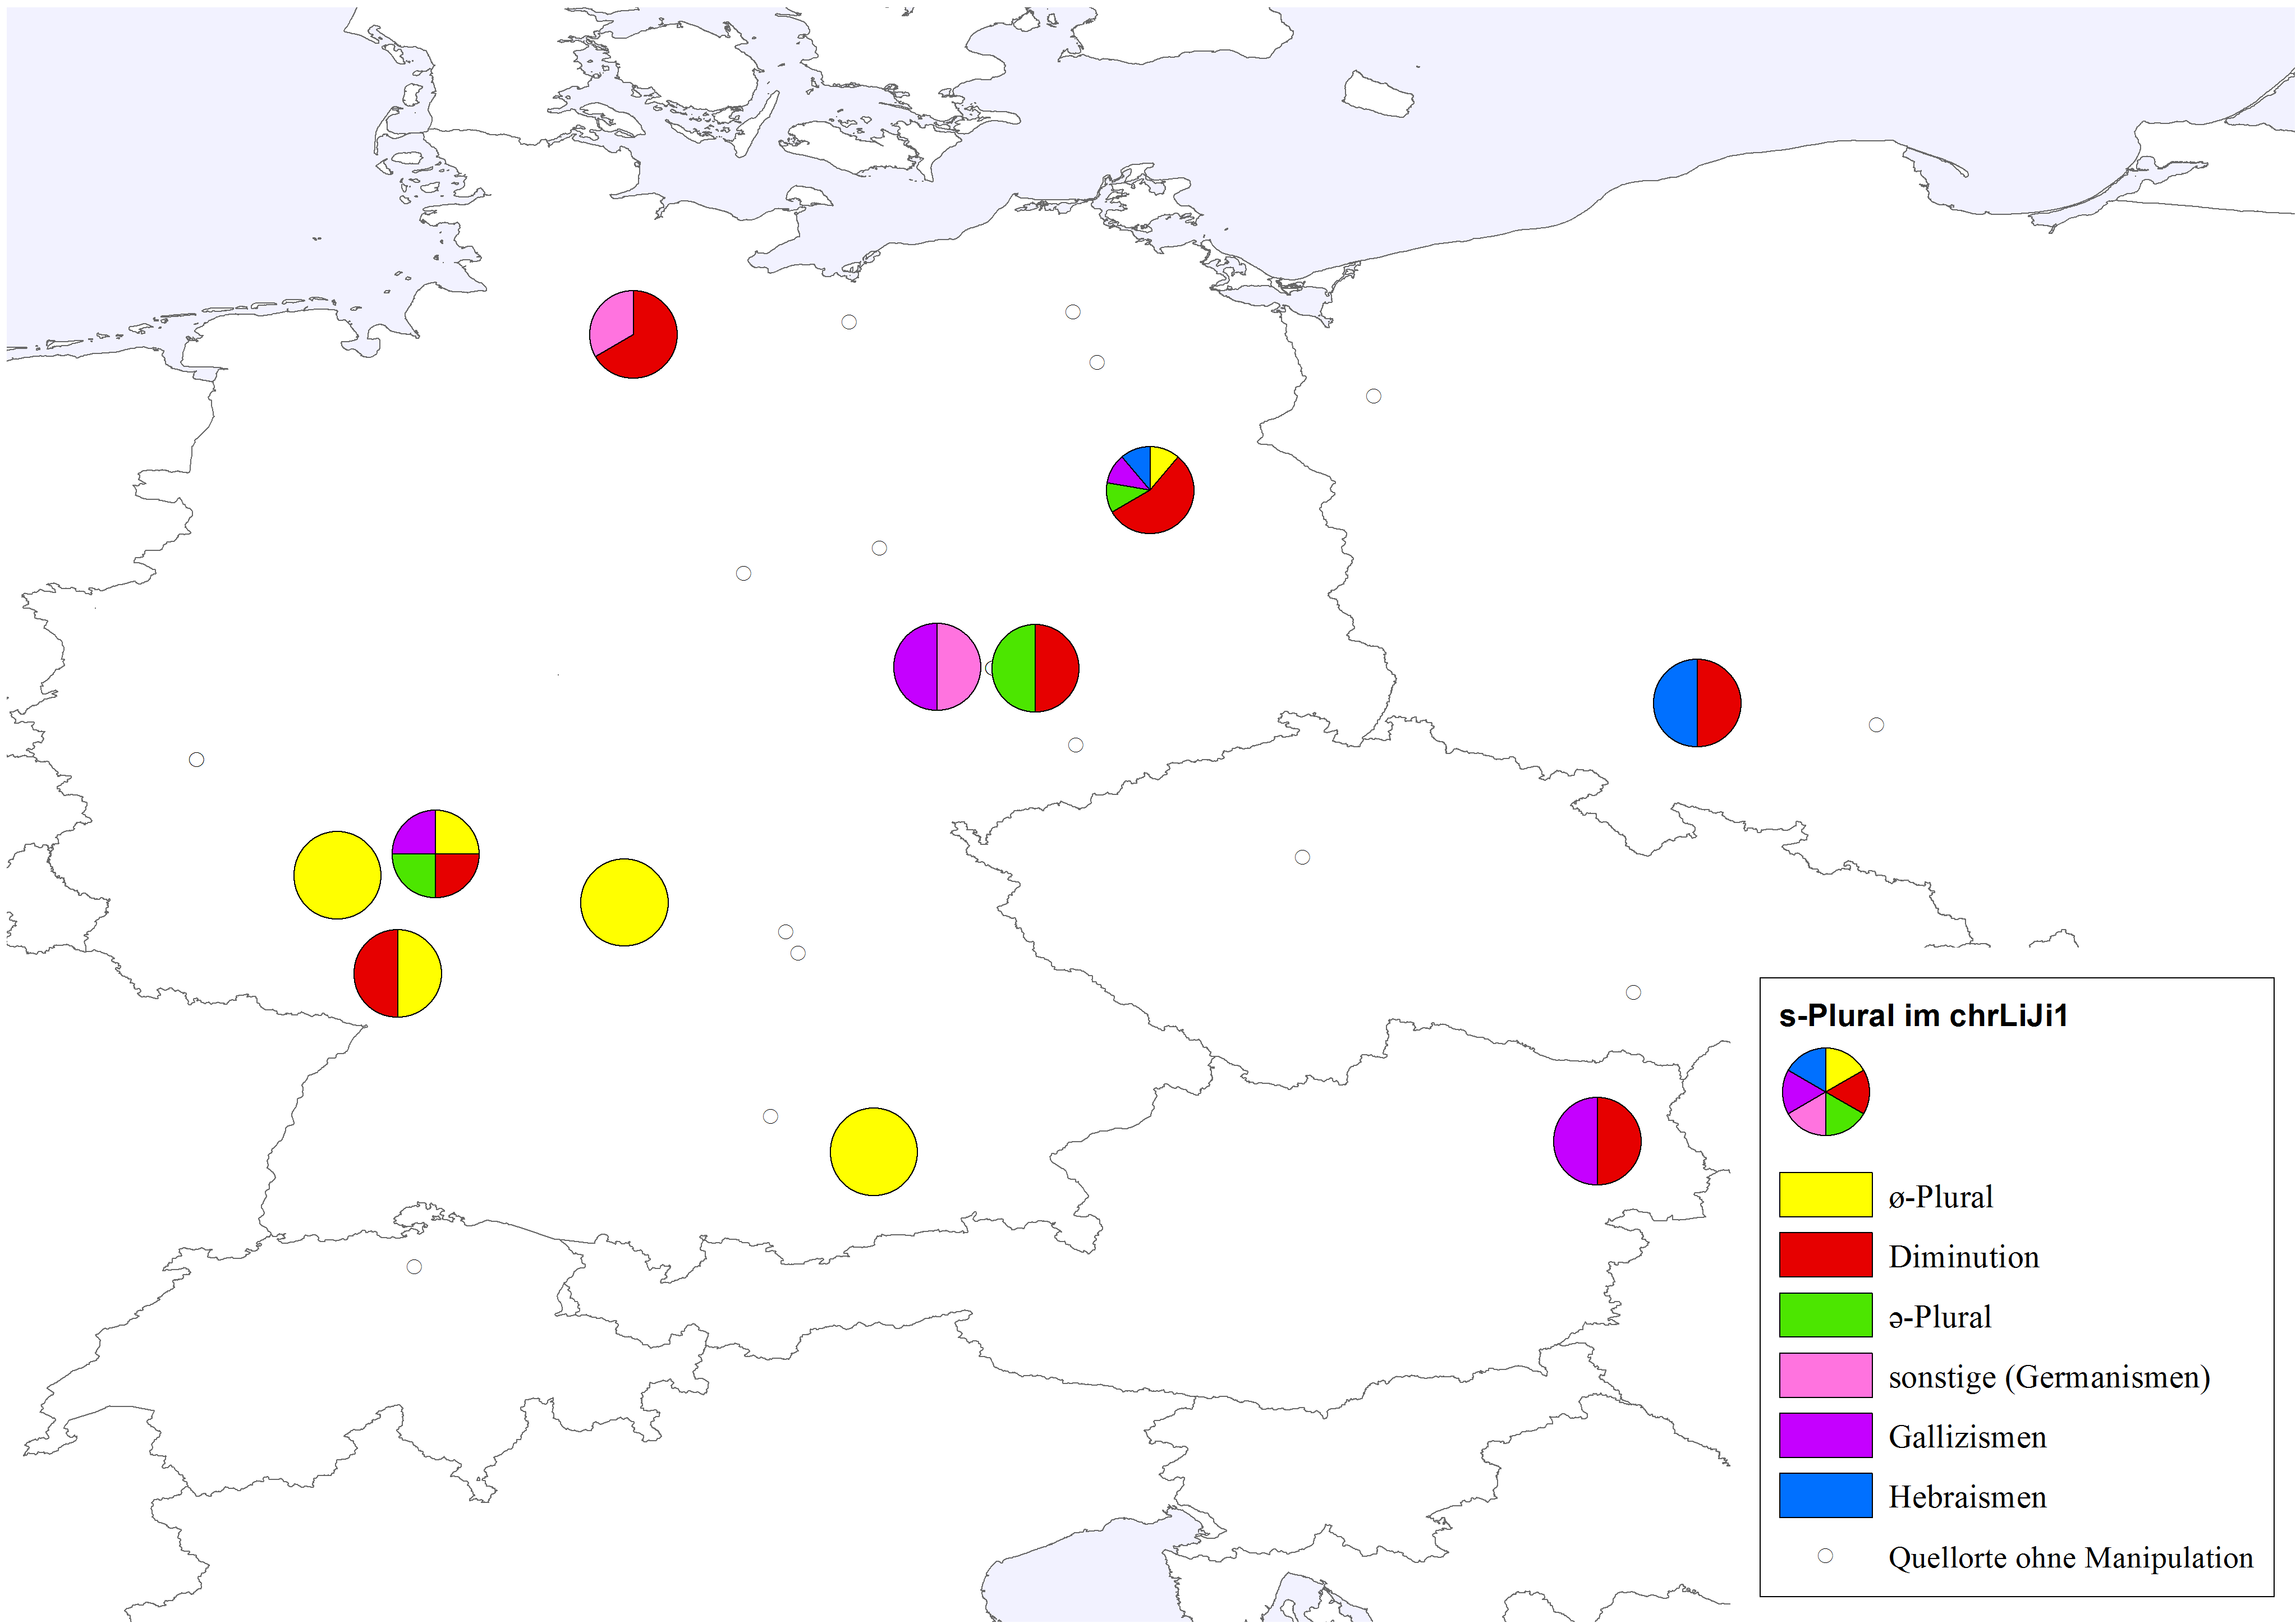
\includegraphics[width=\textwidth]{figures/sPluralKUCHEN2.png}
		\caption{\label{sPluralKarte} \textit{s}-Plural im \hai{chrLiJi1}}
		\end{figure}

		
		
		   \begin{table}
%
		\begin{tabularx}{\columnwidth}{QQr}

	\lsptoprule
\textbf{Typen} & \textbf{Belege} [Pluralsuffix im mod. \hai{{\OJ}}]& \textbf{Quellen}   \\ \midrule
\textbf{nhd. ∅-Plural}  &
\textit{Fischers} \sem{Fischer\textsubscript{{\Pl}}} (\hai{PG}:\,63) [{\oj} \RL{-ס}]; %\ili{OJ}
\textit{Feuerzettels} \sem{Feuerzettel\textsubscript{{\Pl}}} (\hai{NW}:\,9) [{\oj} \RL{-ען}]; \textit{Frackärmels} \sem{Frackärmel\textsubscript{{\Pl}}} (\hai{SV}:\,6) [{\oj} ∅-] \textit{Busens} \sem{Busen\textsubscript{{\Pl}}} (\hai{VD}:\,16) [{\oj} \RL{-ס}]; %\ili{OJ}  
& 4 \\


\textbf{alte Kollektiva (nhd. ∅-Plural)}  &
\textit{Gelärms} \sem{Gelärme\textsubscript{{\Pl}}} (\hai{FL}:\,38)\,[{\oj} –]; 
\textit{Gelafs} \sem{Gelaufe\textsubscript{{\Pl}}} (\hai{FL}:\,38) [{\oj} –];\textit{Ungewitters} \sem{Unwetter, Gewitter\textsubscript{{\Pl}}} (\hai{LM}:\,18)  [{\oj} –]; 
 & 2 \\

\textbf{\isi{Diminution}  (schriftl. nhd. ∅-Plural; {\oj} \RL{לעך}-, \RL{עלעך}-)}  & z.\,B.\, \textit{Blümches} \sem{Blume\textsubscript{{\Dim} {\Pl}}} (\hai{MV}:\,152), \textit{Baanches} \sem{Bein\textsubscript{{\Dim} {\Pl}}} (\hai{PG}:\,44), \textit{Gesellschaftges} \sem{Gesellschaft\textsubscript{{\Dim} {\Pl}}} (\hai{PA}:\,23),  \textit{Schicksels} \sem{Schickse\textsubscript{{\Dim} {\Pl}}, Nichtjüdin\textsubscript{{\Dim} {\Pl}}} (\hai{BP}:\,6; \hai{JP}:\,44), \textit{Gomolches} \sem{Kamel\textsubscript{{\Pl}}} (\hai{NW}:\,33) & 13 \\


\textbf{ə-Plural} &  
\textit{Kerls} \sem{Kerl\textsubscript{{\Pl}}} (\hai{VD}:\,18; \hai{AD}:\,138) [{\oj} –];  \textit{Schnauzbarts} \sem{Schnauzbart\textsubscript{{\Pl}}} (\hai{AD}:\,139) [{\oj} ∅-]; \textit{Teppichs} \sem{Teppich\textsubscript{{\Pl}}} (\hai{NW}:\,8) [{\oj} \RL{-ער}]; 
 & 3\\  



\textbf{Hebraismen}  &
\textit{Gois} \sem{Nichtjude\textsubscript{{\Pl}}} (\hai{JK}:\,27) [{\oj} \RL{-ים}]
 & 1\\



\textbf{Gallizismen}  &
\textit{Dames} \sem{Damen\textsubscript{{\Pl}}} (\hai{NW}:\,71; \hai{PA}:\,5; \hai{TH}:\,135) [{\oj} \RL{-ן}\,\RL{-ס}]; %\ili{OJ}    
\textit{Cavalierers} \sem{Cavalier\textsubscript{{\Pl}}} (\hai{DW}:\,71) [{\oj} –] & 4\\



\textbf{Sonstige}  &
\textit{Herrens} \sem{Herr\textsubscript{{\Pl}}} (\hai{TH}:\,135) \mbox{[{\oj} –]};
\textit{Ette's} \sem{Vater\textsubscript{{\Pl}}} (\hai{JP}:\,44) [Lexem nicht im {\oj} vorhanden] & 2 \\ \lspbottomrule

 \end{tabularx}
		 \caption{\textit{s}-Plurale im \hai{chrLiJi1}}
		 \label{tblsPLURAL}
		 \end{table}

 


Obwohl aus den authentischen Quellen des Westjiddischen keine auffällige Verwendung des Plural-\textit{s} bekannt ist, finden sich im \hai{jüdLiJi1} sehr wohl Belege, die denen des \hai{chrLiJi1} ähneln (vgl.\, \ref{bspSjürliji1_1}–\ref{bspSjürliji1_8}). Unter den acht Belegen finden sich auch zwei Fälle, in denen ein \textit{s}-Plural dem ostjiddischen Standard entspräche (\ref{bspSjürliji1_3}), (\ref{bspSjürliji1_4}). Besonders frequent sind auch hier \textit{s}-Plurale bei nhd. ∅-Plural (\ref{bspSjürliji1_1}–\ref{bspSjürliji1_4}).  Der \textit{en}-Plural findet sich gehäuft im Lexem \sem{Junge} in den \hai{GuS} (\ref{bspSjürliji1_5}). Für Plural-\textit{s} anstelle \,%rs Duden empfiehlt "anstelle"
des Schriftdeutschen ə-Plurals gibt es nur einen Beleg im \hai{jüdLiJi1} (\ref{bspSjürliji1_8}). Besonders augenscheinlich an den Belegen für den \textit{s}-Plural im \hai{jüdLiJi1} ist, dass er ausschließlich in den Berliner Quellen, also umgeben vom niederdeutschen Substrat, auftritt, nicht aber in den Quellen aus dem ostmitteldeutschen bzw. ungarischen Raum. Da der \textit{s}-Plural im Niederdeutschen äußerst \isi{produktiv} ist (vgl.\, \citealt[147–150]{Lindowetal1998}), liegt es nahe, diese Belege als Interferenz mit dem deutschen Dialekt zu deuten. 

 
Die Daten aus den zwei Korpora deuten einen Rückgang an \textit{s}-Pluralen im \hai{{\LiJi}} an. Die Funktion des \textit{s}-Plurals im Literaturjiddischen bleibt fragwürdig. Denkbar sind neben tatsächlichen Imitationen des (Ost-)Jiddischen auch Interferenzen mit den deutschen Dialekten. Zumindest im niederdeutschen Raum ist dies durchaus plausibel. Aber auch eine Markierung der Sprache als \quein{fremd} und besonders als \quein{mit-dem-Französischen-sympathisierend} kann mit Hilfe der \textit{s}-Plurale beabsichtigt sein.

\eenumsentence{
\item \textit{Italieniers} \sem{Italiener\textsubscript{{\Pl}}} (\hai{GuS1}:\,3); vgl.\, {\oj} ∅-\RL{איטא\makebox(-1.5,-7.5)[r]{\libertineGlyph{uni207B}}ליענער} \textit{italiener-∅} \label{bspSjürliji1_1}
\item \textit{Kellers} \sem{Keller\textsubscript{{\Pl}}} (\hai{GuS5}:\,4); vgl.\, {\oj} \RL{קעלער-ן} \textit{keler-n}\label{bspSjürliji1_2}
\item \textit{Schreibers} \sem{Schreiber\textsubscript{{\Pl}}} (\hai{PBerlin1}:\,4); vgl.\, {\oj} \RL{שר{יי}\makebox(-1.5,-3.5)[r]{\libertineGlyph{uni207B}}בער-ס} \textit{shrayber-s}\label{bspSjürliji1_3} %\ili{OJ}
\item \textit{Bergers} \sem{Bürger\textsubscript{{\Pl}}} (\hai{PBerlin2}:\,1.Sp., 2.Sp.); vgl.\, {\oj} \RL{בירגער-ס} \textit{birger-s}\label{bspSjürliji1_4} %\ili{OJ}
 


\item \textit{Jungens} \sem{Junge\textsubscript{{\Pl}}} (\hai{GuS10}:\,11; \hai{GuS15}:\,5; \hai{GuS23}:\,4); vgl.\, {\oj} \RL{{{יי}\makebox(-1.5,-5.5)[r]{\libertineGlyph{afii57807}}}נגל-עך} \textit{jingl-ekh}\label{bspSjürliji1_5}


 \item \textit{Schtrümps} \sem{Strumpf\textsubscript{{\Pl}}} (\hai{PBerlin2}:\,1.Sp.); vgl.\, {\oj} \RL{שטריפ-∅} \textit{shtrimp-∅}\label{bspSjürliji1_8} 

}


\subsection{Der \textit{er}-Plural im \hai{{\LiJi}}}\label{erPLURAL}
%  %\noindent
Neben dem starken Gebrauch von \textit{s}-Pluralen und Diminutivpluralen zeigt das \hai{{\LiJi}} wenig Abweichungen vom Schriftdeutschen bei der Pluralbildung. Ein weiteres Phänomen deutet sich jedoch bereits im Rahmen der Pluraldiminution an (vgl.\, Unterabschnitt \ref{dimsg}). Eine häufige Strategie zur Bildung eines Pluraldiminutivums (im \hai{{\LiJi}} wie auch in den dt. Dialekten) ist die Addition des Pluralmorphems \textit{-er} an ein Diminutivsuffix, z.\,B.\, in \textit{Stickelcher} \sem{Stück\textsubscript{{\Dim} {\Pl}}} (\hai{VD} Frankfurt, 1916:\,17, vgl.\, Tabelle \ref{tblDIMPL}). Der \textit{er}-Plural findet sich auch bei der normalen Pluralbildung in zwei Quellen des \hai{chrLiJi1} an schriftsprachlich untypischen Positionen (\ref{bspERliji_1})--(\ref{bspERliji_2}) und im \hai{jüdLiJi1} in zumindest einem Beleg (\ref{bspERjüdliji}). Immerhin einer der drei Belege entspricht der Pluralbildung des modernen Ostjiddischen (\ref{bspERliji_2}). 

Aus \qu{Der Hochzeit zu Grobsdorf} kann eine besondere Verwendung dieses Pluralmorphems zumindest in Diminutiva (\ref{bspERgrob0}) und erstarrten Diminutiva (\ref{bspERgrob}) nachgewiesen werden. In Kontexten wie etwa (\ref{bspERliji_1}) findet es sich jedoch nicht (\ref{bspERgrob2}). 
Eine besondere Profilierung des \textit{er}-Plurals wäre vor allem im Mitteldeutschen und den koterritorialen jiddischen Varietäten anzunehmen. Der Beleg der fränkischen Quelle aus, vgl. (\ref{bspERliji_1}) könnte somit unter Umständen tatsächlich auf eine Sprachrealität, wenn auch auf eine deutsch-dialektale, verweisen.


\eenumsentence{
\item \textit{Bahner} \sem{Bein\textsubscript{{\Pl}}} (\hai{GP} Nürnberg, 1831:\,28); vgl.\, {\oj} \RL{ביין-ער} \textit{beyn-er} \sem{Knochen} (vgl.\, Fn. \ref{fuss} S.\, \pageref{fuss})\label{bspERliji_1} %Nürnberg

\item \textit{Teppicher} \sem{Teppich\textsubscript{{\Pl}}} (\hai{AK} Zürich, 1948:\,224); vgl.\, {\oj} \RL{טע{פ\makebox(-1,4)[r]{\libertineGlyph{afii57807}}}עך-ער} \textit{tepekh-er}\label{bspERliji_2}
%\ili{OJ}! vgl.\, AK hat auch n-Plural

\item \textit{Menscher} \sem{Mensch\textsubscript{{\Pl}}}(\hai{GuS5}:\,5);  vgl.\, {\oj} \RL{מענטש-ן} \textit{mentsh-n} \label{bspERjüdliji}

\item \RL{ווייבערכער} \textit{weibercher} \sem{Weib\textsubscript{{\Dim} {\Pl}}}\\
(\qu{Die Hochzeit zu Grobsdorf} 1822:\,85)\label{bspERgrob0}

\item \RL{מערערכער} \textit{merercher} \sem{Mädchen\textsubscript{({\Dim}) {\Pl}}}\\ 
(\qu{Die Hochzeit zu Grobsdorf} 1822:\,70, 74, 90, 92, 95)  \label{bspERgrob}

\item \RL{בא\makebox(-1.5,-7.5)[r]{\libertineGlyph{uni207B}}ה} \textit{bah} \sem{Bein\textsubscript{{\Pl}}} (\qu{Die Hochzeit zu Grobsdorf} 1822:\,12)\footnote{Es handelt sich hier um einen ∅-Plural (keine \isi{Subtraktion}); vgl.\, \RL{בא\makebox(-1.5,-7.5)[r]{\libertineGlyph{uni207B}}ה} \textit{bah} \sem{Bein\textsubscript{{\Sg}}} (\qu{Die Hochzeit zu Grobsdorf} 1822:\,69).} \label{bspERgrob2}

}


\subsection{Der \textit{en}-Plural im \hai{{\LiJi}}}\label{enPLURAL}
%  %\noindent
Desweiteren finden sich in wenigen Quellen Belege für den \textit{en}-Plural, wo er im Schriftdeutschen nicht verwendet wird. So etwa in einer niederdeutschen Quelle (\ref{bspENliji_1}), \,%rs Spatum fehlt
 in der eine Interferenz mit dem deutschen Dialekt anzunehmen ist. Im \hai{chrLiJi1} finden sich wenige, einzelne Belege in vier Quellen (\ref{bspENliji_1}–\ref{bspENliji_5}); Im \hai{jüdLiJi1} (\ref{bspENjüliji1_1}) in einer Quelle. In (\ref{BSPENPL}) sind alle Belege für untypische \textit{en}-Plurale in den beiden Korpora angeführt. Es fällt dabei auf, dass dieses Suffix überwiegend an der Position von schriftsprachlich -ə (+ \isi{Umlaut}) steht (\ref{bspENliji_1}), (\ref{bspENliji_5}). Die beiden übrigen Belege (\ref{bspENliji_3} u. \ref{bspENliji_4}) betreffen mit einem \isi{Hebraismus} ein \isi{Fremdwort}. Immerhin zwei der fünf Quellen des \hai{chrLiJi1}, die einen von der Schriftsprache abweichenden \textit{-(e)n} Plural in jüdischer Figurenrede verwenden, entsprechen damit der ostjiddischen Form (\ref{bspENliji_1} u. \ref{bspENliji_5}), wenngleich ein niederdeutscher Einfluss im Beleg \ref{bspENliji_1} der Quelle \hai{UT} (Stavenhagen, 1862) nicht auszuschließen ist. Die Quelle \hai{AK} (Zürich, 1948), die bereits bei der Verwendung des ostjiddischen \textit{er}-Plurals aufgefallen ist (\ref{bspENliji_5}), zeigt auch hier die \quein{korrekte} {\oj} Pluralform (\ref{bspERliji_2}, S.\, \pageref{bspERliji_2}). 

 \eenumsentence{\label{BSPENPL}
 
\item \textit{Gerichten} \sem{Gericht\textsubscript{{\Pl}}} (\hai{UT} Stavenhagen, 1862:\,Kap.\, 3); vgl.\, {\oj} \RL{געריכט-ן} \textit{gericht-n}\label{bspENliji_1}

\item \textit{Goyen} \sem{Christ, Goy\textsubscript{{\Pl}}} (\hai{MS} Bonn, 1822:\,363L); vgl.\, {\oj} \RL{גוי-ם} \textit{goy-im} \label{bspENliji_3}

\item \textit{Schabbesgoien} \sem{Christ, Goy\textsubscript{{\Pl}}} (\hai{JK} Breslau, 1810:\,13); vgl.\, {\oj} s.\,o.\label{bspENliji_4} %ls! hier wäre die genaue Stelle von s.o. schön

 \item \textit{Kanaln} \sem{Kanal\textsubscript{{\Pl}}} (\hai{AK} Zürich, 1948:\,247); vgl.\, {\oj} \RL{קא\makebox(-1.5,-7.5)[r]{\libertineGlyph{uni207B}}נא\makebox(-1.5,-7.5)[r]{\libertineGlyph{uni207B}}ל-ן} \textit{kanal-n}\label{bspENliji_5}%\ili{OJ}


\item \textit{Tellern} \sem{Teller\textsubscript{{\Pl}}} (\hai{GuS23}:\,13); vgl.\, {\oj} \RL{טעלער-∅} \textit{teler-∅}\label{bspENjüliji1_1}

}


 
 \section{Flexion von Eigennamen}\label{dativnamen}
 %\noindent
 Jiddisch flektiert den \isi{Dativ} und z.\,T. auch den \isi{Akkusativ} bei \isi{Eigennamen}, Familientermini und pränominalen Genitiven mittels der Suffigierung von -\textit{n} (\citealt[161f]{Jacobs2005};vgl.\, \ref{dativOJ1}–\ref{dativOJ2}). \cite[161]{Jacobs2005} spricht hier von einem obliquen Kasus. Seinen Ursprung haben diese Formen in der germanischen Komponente der schwachen \isi{Flexion} bei \isi{Eigennamen} des Alt- und Mittelhochdeutschen (vgl.\, \citealt[insbes. 230f]{Nuebling2012}). Im Schriftdeutschen ging diese Eigennamenflexion, die durch Suffigierung von \textit{-e(n)} [± \isi{Umlaut}] erfolgte, im Verlauf des 19. Jahrhunderts vollständig verloren und wurde von Bildungen, die nun nur mehr den Plural vom Singular mittels \textit{-s}-Suffigierung markieren, abgelöst (z.\,B.\, \ref{BSPsNAME}, vgl.\, \citealt[240]{Nuebling2012}).\footnote{In erstarrter Form erhalten blieb die alte \isi{Flexion} im Gegenwartsdeutsch – wohl aufgrund des Reimes – in der Phrase \textit{Futtern wie bei Muttern}.} In den hochdeutschen Mundarten blieben die alten Formen zum Teil konserviert. Bekannt ist dies etwa für die bairischen Mundarten Tirols (z.\,B.\, \ref{BSPDATIVTIROL}, vgl.\, \citealt[50]{Schatz1903}). Defizitär, aber wesentlich vitaler ist die Eigennamenflexion mittels \textit{-e(n)} noch in friesischen und niederländischen Dialekten (\citealt{Hoekstra2010}). Im Niederdeutschen ist die Eigennamenflexion jedoch nur mehr im pränominalen \isi{Genitiv} üblich (vgl.\, \citealt[144]{Lindowetal1998}). 

 Im \hai{chrLiJi1} finden sich in zwei Quellen insgesamt drei Belege für die Eigennamenflexion an männlichen Vornamen (\ref{dativ1})--(\ref{dativ2.2}). Nur ein Beleg für die \isi{Flexion} eines weiblichen Vornamens tritt im \hai{jüdLiJi1} auf (\ref{dativ3}). Dieses Phänomen ist damit generell kein frequentes Mittel zur Figurenmarkierung im \hai{{\LiJi}}. Was es dennoch bemerkenswert macht, ist, dass es ausschließlich in nord-östlichen Quellen (Pyritz, Stavenhagen, Berlin), darunter die beiden niederdeutschen Quellen des \hai{chrLiJi1}-\isi{Korpus}, belegt ist. In Fritz Reuters \hai{UT} (Stavenhagen, 1862) findet sich die \isi{Flexion} von \isi{Eigennamen} auch im sprachlich unmarkierten Text, z.\,B.\, \ref{UTFRITZENNDT}. Man könnte nun annehmen, dass hier der ostjiddische Einfluss mitunter stärker gewirkt haben mag, als andernorts. Viel wahrscheinlicher, als ein ostjiddischer Einfluss ist im vorliegenden Fall aber eher eine Entlehnung aus dem umliegenden Niederdeutschen.
 


\eenumsentence{

\item \RL{ר{ב\makebox(-0.8,9)[r]{\libertineGlyph{uni207B}}}קהן} \textit{rivken} \sem{Rebekka\textsubscript{{\Dat}/{\Akk}}} (zitiert n. \citealt[161]{Jacobs2005})\label{dativOJ1} 

\item \RL{ב{א\makebox(-1.25,-1.25)[r]{\libertineGlyph{uni05B8}}}בן} \textit{bobn} \sem{Großmutter\textsubscript{{\Dat}/*{\Akk}}} (zitiert n. \citealt[161]{Jacobs2005})\label{dativOJ2} 

 \item \textit{Die zwei Peters} \sem{Die zwei Peter\textsubscript{{\Pl}}} (vgl.\, \citealt[240]{Nuebling2012})\label{BSPsNAME}
 
 \item \textit{i soks föttərn} \sem{ich sage es dem Vetter\textsubscript{{\Dat}}} (Ötztal, zitiert n. \citealt[50]{Schatz1903})\label{BSPDATIVTIROL}
 
\item \textit{Würd Mosissen dat doch geling'n}  
 \sem{würde Moses\textsubscript{{\Dat}} das doch gelingen} (\hai{DP} Pyrzyce, 1874:\,9)\label{dativ1} %Pyritz Sprache Niederdeutsch
 
 \item \textit{Rufen Sie Daviden} \sem{Rufen Sie David\textsubscript{{\Akk}}}(\hai{UT} Stavenhagen, 1862:\,Kap.\, 45) %Niederdeutsch
 
 \item \textit{\qu{Frau Pastorin}, säd Bräsig, \qu{mit Mosessen, das is woll 'ne bloße Erscheinung for Sie gewesen}}  
 \sem{\quein{Frau Pastorin}, sagt Bräsig, \quein{das mit Moses\textsubscript{{\Dat}} ist wohl eine bloße Erscheinung für Sie gewesen.}} (\hai{UT} Stavenhagen, 1862:\,Kap.\, 45)\label{dativ2.2}%Niederdeutsch

 
  \item \textit{Grüße mir Riwken} \sem{Grüß mir Rebekka\textsubscript{{\Akk}}} (\hai{GuS1}:\,6)\label{dativ3} %jüd\ili{LiJi1} = Berlin
 
 
 \item \textit{Hawermann was desen Morgen mit Franzen nah Gürlitz tau Kirchen gahn} 
 \sem{Hawermann war diesen Morgen mit Franz\textsubscript{{\Dat}} nach Gürlitz zur Kirche gegangen} (\hai{UT} Stavenhagen, 1862:\,Kap.\, 11)\label{UTFRITZENNDT}
 }
 
 \section{Kasussynkretismen}\label{kasus} 
%\noindent
 Das Kasussystem des modernen Ostjiddischen unterscheidet sich in vielfacher Weise vom Deutschen (vgl.\, \citealt[154–222]{Jacobs2005}) und auch das Westjiddische zeigt einige dieser aus dem Ostjiddischen bekannten Strukturen (vgl.\, \citealt{Fleischer2014,FleischerSchaefer2012}; \citealt[61–66]{Reershemius2007}).  So verwundert es kaum, dass auch im \hai{{\LiJi}} Unterschiede gegenüber dem Schriftdeutschen im Bereich der Kasus zu finden sind.
  
\cite[102]{Richter1995} stellt in den von ihm untersuchten Quellen des \hai{{\LiJi}} den häufigen Gebrauch \qu{des Akkusativs anstelle des Dativs} fest. Er geht jedoch nicht näher auf die einzelnen Belege ein. Im \isi{Korpus} zum \hai{chrLiJi1} konnten Kasussynkretismen in drei Bereichen festgestellt werden: bei vollen Objekten in Nominalphrasen (Unterabschnitt \ref{kasusobj}), bei vollen Objekten in Präpositionalphrasen (Unterabschnitt \ref{kasuspräp}) und bei \isi{Pronomen} in Nominal- und Präpositionalphrasen (Unterabschnitt \ref{kasuspron}). Im Folgenden werden damit erstmals systematisch die Abweichungen des \hai{{\LiJi}} vom Schriftdeutschen erfasst und mit den vorhandenen Daten zum West- und Ostjiddischen verglichen.

 \subsection{Kasus bei vollen Objekten}\label{kasusobj}

Zum Kasussystem des Alt- oder Westjiddischen ist noch wenig Genaues bekannt. Die einzige Beschreibung eines westjiddischen Kasussystems, welches deutlich von der niederdeutschen Kontaktsprache gezeichnet ist, liefert bislang \citet[61–66]{Reershemius2007}. Prinzipiell ist anzunehmen, dass sich \ili{Westjiddisch}  in einem ähnlichen Maß, wohl aber in unterschiedlichen Bereichen, vom Schriftdeutschen unterscheidet, wie das Ostjiddische. Da es an Vergleichsdaten fehlt, können lediglich die Situation im Ostjiddischen herangezogen  und die Belegdaten  aus den Korpora des \hai{{\LiJi}} vorgestellt werden. 

 Das Standardjiddische  und -deutsche Kasussystem bei vollen Objekten\footnote{Darunter verstanden werden \hai{{\NP}}s nach dem Muster \textit{\isi{Artikel} (+ \isi{Adjektiv}) + Nomen}.} unterscheidet sich in nur wenigen Punkten. Im Jiddischen ist der Genitivabbau weiter umgesetzt als im Schriftdeutschen, so dass man hier eher vom \quein{Possessiv} als vom \quein{Genitiv} spricht (\citealt[110f]{Wolf1969}; \citealt[172]{Jacobs2005}; \citealt[403f]{Jacobsetal2013}). Im Singular entspricht die Form des Possessivs der des Dativs; im Plural hingegen des Akkusativs. Die zwei weiteren Unterschiede zum Deutschen sind die Synkretismen von {\Akk} {\Sg} {\mask} mit {\Dat} {\Sg} {\mask} zugunsten des Dativs und von {\Dat} {\Pl} mit {\Akk} {\Pl} zugunsten der Nominativ- bzw. Akkusativform. 
 
Das Kasussystem des Standardjiddischen entspricht weitestgehend dem der meisten jiddischen Dialekte (\citealt[129]{Wolf1969}). Eine Ausnahme findet sich im \hai{{\SÜJ}}, wo die Form des {\Dat} {\f} mit der des {\Akk} zusammengefallen ist (\citealt[129]{Wolf1969}). Ein weitaus umfassenderer \isi{Synkretismus} fand im \hai{{\NOJ}} statt, wo \isi{Akkusativ} und \isi{Dativ} zu einem obliquen Objektkasus (\qu{\RL{{א\makebox(-1.25,-1.25)[r]{\libertineGlyph{uni05B8}}}ביעקט-בויגפא\makebox(-1.5,-7.5)[r]{\libertineGlyph{uni207B}}ל}}) zusammengefallen sind (\citealt[160]{Zaretski1929}; \citealt[117]{Wolf1969}).\label{FNKASUSDIALEKT} \\
 

 \begin{table}
%\begin{longtable}{ccc|ccc}

		\begin{tabular}{lllll}

		\lsptoprule

\textbf{Quelle} &\textbf{{\Sg} {\mask}} & \textbf{{\Sg} {\n}} & \textbf{{\Sg} {\f}} &\textbf{{\Pl}}  \\ \midrule 

\hai{LS} & {\Nom} statt {\Akk} & –	& –	& {\Nom}/{\Akk} statt {\Dat}\\

\hai{SS} & {\Dat} statt {\Akk} & –	& –	& –\\ 
 
\hai{AK} & {\Nom} statt {\Akk} & –	& –	& –\\ 
 
  \lspbottomrule
 \end{tabular}
		 \caption{Kasussynkretismen im \hai{chrLiJi1} bei vollen Objekten}
		 \label{tblOBJKASUS}
		 \end{table}
         
         
	Tabelle \ref{tblOBJKASUS} fasst alle Typen von Kasussynkretismen im \hai{chrLiJi1} zusammen. Eine Quelle (\ref{SS_DAT}) setzt tatsächlich den ostjiddischen \isi{Zusammenfall} im {\Sg} {\mask} um und eine weitere (\ref{LS_PL}) zeigt den \isi{Synkretismus} von {\Akk} und {\Dat} im Plural. Daneben zeigt diese Quelle im Beleg (\ref{LS_NOM}) zumindest in einer Position Manipulationen, wo sich das Ostjiddische vom Schriftdeutschen unterscheidet ({\Sg} {\mask} {\Akk}), wenn auch der ostjiddische \isi{Synkretismus} nicht den Nominativ betrifft. Hier ließe sich eine Hypernorm analog zum Plural (\ref{LS_PL}) annehmen. Für die Quelle \hai{AK} (Zürich, 1948) kann man von einer Interferenz mit dem Alemannischen ausgehen, wo sich der {\Nom}-{\Akk}-\isi{Synkretismus} durchgesetzt hat (vgl.\, \citealt[665f]{Schirmunski1962};s. \ref{AK_NOM}).

\eenumsentence{
\item \textit{ich hob doch gekennt} [\textit{Ihrem Tate}]\textsubscript{{\Dat}} \textit{und Ihre Mammele} (\hai{SS} Berlin, 1907:\,9)\\
\sem{ich habe doch [Ihren Vater]\textsubscript{{\Akk}}  und Ihre Mutter gekannt}\label{SS_DAT}


\item \textit{Helf ich} [\textit{die Lait}]\textsubscript{{\Nom}/{\Akk}} \textit{aus der Not} (\hai{LS} Bonn, 1925:\,13)\\
\sem{Helfe ich [den Leuten]\textsubscript{{\Dat}} aus der Not}\label{LS_PL}

\item \textit{und laß mer nicht nehme} [\textit{mei ehrlicher Name}]\textsubscript{{\Akk}} (\hai{LS} Bonn, 1925:\,4)\\
\sem{und lasse mir nicht [meinen ehrlichen Namen]\textsubscript{{\Dat}} nehmen}\label{LS_NOM}


\item \textit{Madam varstehn} [\textit{kein Spaß}]\textsubscript{{\Nom}}\textit{?}  (\hai{AK} Zürich, 1948:\,235)\\
\sem{Madam verstehen [keinen Spaß]\textsubscript{{\Akk}}?}\label{AK_NOM}

}


Für einen ostjiddischen Einfluss spricht besonders die diachrone Verteilung der Belege (s. Abbildung \ref{histokasusNP}). Aber auch die geographische Lage der Quelle \hai{SS} (Berlin, 1907) spräche für einen möglichen Kontakt zum Ostjiddischen. Manipulationen des Kasus bei vollen Objekten sind beinahe ausschließlich in Quellen des 20. Jahrhunderts belegt.

  
  \begin{figure} 
\fittable{
	\begin{tikzpicture}
		\begin{axis}[only marks, width=0.82\textwidth,height=0.2\textheight,
		legend style={at={(1,1)},xshift=+0.2cm, yshift=-0.1cm,anchor=north west,nodes=left},
			xtick={1700, 1725, 1750, 1775, 1800, 1825, 1850, 1875, 1900, 1925, 1950, 1975}, ytick=\empty,
			x tick label style={/pgf/number format/1000 sep=}, 
			y tick label style={/pgf/number format/1000 sep=},
			extra y tick style={grid=major,
				tick label style={, ,}},
				ymin=0.7,
				ymax=3.5,
			ylabel={Phänomenbelege},
			enlarge x limits=0.03]	
	
\addplot [mark=square*, black] table [x=jahr, y=PL_NOM] {figures/KASUS_NP_PL_NOM.txt};			


\addplot [mark=square*, gray] table [x=jahr, y=SG_M_DAT] {figures/KASUS_NP_SG_M_DAT.txt};


\addplot [mark=*, gray] table [x=jahr, y=SG_M_NOM] {figures/KASUS_NP_SG_M_NOM.txt};



\addplot [mark=o,black] table [x=jahr, y=NO] {figures/KASUS_NP_NO.txt};%1.5
 

						\legend{{\Akk} statt {\Dat} {\Pl}, {\Nom} statt {\Akk} {\Sg}{\mask}, {\Dat} statt {\Akk} {\Sg}{\mask}, keine Manipulation} %macht Legende
		\end{axis}
	\end{tikzpicture}
}
	\caption{Diachrone Verteilung von Kasussynkretismen bei vollen Objekten im \hai{chrLiJi1}}
	\label{histokasusNP}	
\end{figure}



Doch auch ein deutsch-dialektaler Einfluss ist nicht auszuschließen. Den Daten \citeauthor{Shrier1965}s (\citeyear{Shrier1965}) zufolge können zumindest die Singularbelege auf koterritoriale Formen zurückgeführt werden: So findet sich der \isi{Zusammenfall} von \isi{Akkusativ} und Nominativ (beim {\Sg} {\mask}) im gesamten Südwesten (Alemannisch, Mosel- u. Rheinfränkisch und z.\,T.\, im Brandenburgischen; \citealt[423f]{Shrier1965}).\, Die zwei Quellen des \hai{chrLiJi1}, die diesen \isi{Synkretismus} zeigen, stammen aus Zürich und Bonn, also eben jenen Regionen. Der \isi{Zusammenfall} von \isi{Akkusativ} und \isi{Dativ} (beim {\Sg} {\mask}) findet sich hingegen besonders im Ostmitteldeutschen, im gesamten Niederdeutschen und in Teilen des Mittel- und Südbairischen (\citealt[423f]{Shrier1965}). Die Quelle, die diesen \isi{Synkretismus} aufweist, stammt aus Berlin und damit wiederum aus eben jenem Gebiet, in dem der Akkusativ-Dativ-\isi{Synkretismus} auch bei den Pronomina recht prominent ist. Wenn auch sicherlich nicht beabsichtigt, so mag unterschwellig die eigene Dialekt- bzw. Regiolektkompetenz der einzelnen Autoren in die Imitationen hinein gespielt haben.
 

Abschließend lässt sich festhalten, dass Kasusmarkierungen am vollen Objekt im \hai{{\LiJi}} ein eher peripheres Phänomen darstellen. In wenigen Fällen konnten Synkretismen, die aus dem Ostjiddischen bekannt sind, nachgewiesen werden. Die sich mittlerweile andeutende Tendenz des \hai{{\LiJi}}, sich morphosyntaktisch stärker als etwa phonologisch am Ostjiddischen zu orientieren, könnte sich auch hier bestätigt sehen. Um die Situation jedoch sicher bewerten zu können, fehlt es an Daten zu den (west-)jiddischen Dialekten.
 
   \subsection{Kasus nach Präposition}\label{kasuspräp}
  %  %\noindent
  
Im Deutschen regieren Präpositionen die Kasuszuweisung. Dabei hängt diese von den semantischen Bedingungen (statisch vs. direktional) ab (\citealt[23]{PittnerBerman2007}). So fordern Präpositionen in direktionaler \isi{Semantik} den \isi{Akkusativ} (\ref{BSPAKKDIREKTIONAL}); in statischer \isi{Semantik} jedoch den \isi{Dativ} (\ref{BSPDATSTATISCH}). Im modernen Jiddischen hingegen spielt die \isi{Semantik} keinerlei Rolle. Auf eine Präposition folgt immer der \isi{Dativ} (\ref{BSPJIDDIREKT}–\ref{BSPJIDSTAT}) (\citealt[202]{Jacobs2005}; \citealt{FleischerSchaefer2012}). Das ostjiddische Muster vom \isi{Dativ} als \quein{Einheitskasus} nach \isi{Präposition} findet sich ebenso im Süd- und Zentralwestjiddischen z.\,B.\, in (\ref{BspDATGROBS}) (\citealt{FleischerSchaefer2012}; \citealt[24]{GuggenheimGruenberg1966}) und kann als eines der Indizien für die gemeinsame Genese von Ost- und \ili{Westjiddisch} gelten (\citealt{Fleischer2014}).
 
 
 \eenumsentence{


 \item dt. \textit{er geht in die Stadt}\textsubscript{lokal-direktional}\label{BSPDATSTATISCH}
 
  \item dt. \textit{er wohnt in der Stadt}\textsubscript{lokal-statisch}\label{BSPAKKDIREKTIONAL}
 
 
   \item mod. \ili{Ostjiddisch} \textit{er geyt in der shtot}\textsubscript{lokal-direktional}\label{BSPJIDDIREKT}
   
 
  \item mod. \ili{Ostjiddisch} \textit{er voynt in der shtot}\textsubscript{lokal-statisch}\label{BSPJIDSTAT}

  
 \item {\RL{איץ ווא\makebox(-1.5,-7.5)[r]{\libertineGlyph{uni207B}}רד אופפעם דא\makebox(-1.5,-7.5)[r]{\libertineGlyph{uni207B}}נץ געמא\makebox(-1.5,-7.5)[r]{\libertineGlyph{uni207B}}רשירט} }\\
  \textit{iz ward uffem danz gemarschirt}\textsubscript{lokal-direktional} \\
  \sem{Jetzt wird auf den (wörtl. dem) Tanz marschiert}\\
  (\qu{Die Hochzeit zu Grobsdorf} 1822:\,53) \label{BspDATGROBS}
  
  
  \begin{flushright}
  (\ref{BSPDATSTATISCH}–\ref{BSPJIDSTAT} zitiert n. \citealt[415]{FleischerSchaefer2012};\\
  \ref{BspDATGROBS} vgl.\, \citealt[423]{FleischerSchaefer2012})
    \end{flushright}
 
 
 }
  
   Im Plural sind \isi{Akkusativ} und \isi{Dativ} in Ost- und \ili{Westjiddisch} in die Akkusativform zusammengefallen (vgl.\, Unterabschnitt \ref{kasusobj} S.\, \pageref{kasusobj}). Dies spiegelt sich auch im Kasus nach \isi{Präposition} wider (\citealt{FleischerSchaefer2012}). Von einer jiddischen Varietät ist daher im Plural der \isi{Akkusativ} anstelle des Dativs zu erwarten. 
   Im \hai{{\NOJ}}, wo \isi{Dativ} und \isi{Akkusativ} generell zusammengefallen sind (s.\,o. S.\, \pageref{FNKASUSDIALEKT}; \citealt[160]{Zaretski1929}), verhalten sich hingegen Singular und Plural identisch. Das Jiddische Nordpolens (\citealt{Herzog1965}) und das nordöstliche \ili{Westjiddisch} zeigen ein zum standardostjiddischen komplementäres System (\citealt{FleischerSchaefer2012}; \citealt[130–132]{Herzog1965}). Hier  ist der Einheitskasus nach \isi{Präposition} der \isi{Akkusativ}, nicht der \isi{Dativ}. Ob und wie weit diese Form ins östliche \hai{{\ZWJ}}, \hai{{\SWJ}} bzw. \hai{{\SÜJ}} hineinstreut, konnte aufgrund der dünnen Quellenlage noch nicht geklärt werden. \cite{FleischerSchaefer2012} finden jedoch Anhaltspunkte, dass der \isi{Akkusativ} nach \isi{Präposition} ggf. auch in den dortigen jiddischen Varietäten verbreitet war. Entsprechende Daten, wie sich die deutschen Mundarten flächendeckend beim Kasus nach \isi{Präposition} verhalten, liegen bislang keine vor. 
 
Die Analyse des \hai{{\LiJi}} kann nur \quein{Verstöße} gegen das deutsche Schriftsystem erfassen, also nur die Fälle, in denen der \isi{Dativ} an der Position von deutsch \isi{Akkusativ} erscheint bzw. der umgekehrte Fall eintritt. Hier werden zunächst nur volle \hai{{\NP}}s nach \isi{Präposition} behandelt. Darauf, wie sich \isi{Pronomen} nach Präpositionen im \hai{{\LiJi}} verhalten, wird in Abschnitt \ref{kasuspron} näher eingegangen. Die Tabellen \ref{tblpräpkasus1} und \ref{tblpräpkasusjüdliji}  
geben die Belege dieser Verstöße an. 23 Quellen (43\%) des \hai{chrLiJi1} und 8 (von 10) Quellen des \hai{jüdLiJi1} 
zeigen solcherlei \quein{Verstöße}. 

 \begin{table} 


\fittable{
		\begin{tabular}{lllll}

		\lsptoprule 

\textbf{Quelle} &\textbf{{\Sg} {\mask}} & \textbf{{\Sg} {\n}} & \textbf{{\Sg} {\f}} &\textbf{{\Pl}}  \\ 
\midrule 

\hai{{\PP}} &	–	  &	–	& –	&  {\Akk} $>$ {\Dat}	\\
 
\hai{BW} &	–	  &	{\Dat} $>$ {\Akk}	& –	& –	\\
 
\hai{LM} &	–	  &	–	&	{\Akk} $>$ {\Dat} & –	\\
 
\hai{BP} &	–	  &	{\Dat} $>$ {\Akk}	& –	& {\Dat} $>$ {\Akk}\\
 
\hai{GP} &	–	  &	–	& {\Dat} $>$ {\Akk}	& {\Dat} $>$ {\Akk}	\\
 
\hai{PG} &	–	  &	–	&	{\Dat} $>$ {\Akk};{\Akk} $>$ {\Dat} & {\Dat} $>$ {\Akk} 	\\
 
\hai{TH} &	–	  &	–	&	{\Dat} $>$ {\Akk} & {\Dat} $>$ {\Akk} 	\\
 
\hai{AJ} &	–	  &	{\Dat} $>$ {\Akk}	&	{\Dat} $>$ {\Akk}& {\Dat} $>$ {\Akk}	\\
 
\hai{MS} &	–	  &	–	& –	& {\Akk}	\\
 
\hai{PA} &	–	  &	–	& {\Dat} $>$ {\Akk}	& –	\\
 
\hai{WA} &	–	  &	{\Dat} $>$ {\Akk}	&	{\Dat} $>$ {\Akk} &  {\Dat} $>$ {\Akk};{\Akk} $>$ {\Dat}	\\
 
\hai{UT} ({\ndt})&	–	  &	{\Dat} $>$ {\Akk}	& –	& 	{\Dat} $>$ {\Akk}\\
 
\hai{AB} &	–	  &		{\Dat} $>$ {\Akk}& –	& –	\\
 
\hai{JP} &	–	  &	{\Dat} $>$ {\Akk}	&	{\Dat} $>$ {\Akk}& –	\\
 
\hai{SS} &		{\Akk} $>$ {\Dat}  &	–	& –	& –	\\
 
\hai{FL} &	–	  &	–	&{\Dat} $>$ {\Akk}	& {\Dat} $>$ {\Akk}	\\
 
\hai{VD} &	–	  &		{\Akk} $>$ {\Dat} &	{\Akk} $>$ {\Dat} & {\Dat} $>$ {\Akk}	\\
 
\hai{AD} &	–	  &	–	&	{\Dat} $>$ {\Akk}& {\Dat} $>$ {\Akk}	\\
 
\hai{MV} &	–	  &{\Dat} $>$ {\Akk}&{\Dat} $>$ {\Akk}	& –	\\
 
 \hai{DG} &	–	  &	–	&	{\Dat} $>$ {\Akk}& {\Dat} $>$ {\Akk}	\\
 
\hai{GW} &	–	  &	{\Akk} $>$ {\Dat}	& –	& –	\\
 
 \hai{SV} &	–	  &	{\Dat} $>$ {\Akk}	& –	& –	\\
 
 \hai{AK} &	{\Dat} $>$ {\Akk}  &	{\Dat} $>$ {\Akk}	& –	& {\Dat} $>$ {\Akk}	\\
  \lspbottomrule
 \end{tabular}
}
		 \caption{Diachrone Verteilung von Verstößen gegen das schriftdeutsche Kasussystem im \hai{chrLiJi1} bei Präpositionalphrasen}
		 \label{tblpräpkasus1}
		 \end{table}


	 \begin{table}


\fittable{
		\begin{tabular}{lllll}

		\lsptoprule 

\textbf{Quelle} &\textbf{{\Sg} {\mask}} & \textbf{{\Sg} {\n}} & \textbf{{\Sg} {\f}} &\textbf{{\Pl}}  \\ \midrule 

 \hai{GuS1} &	–	  &	{\Dat} $>$ {\Akk}		& {\Dat} $>$ {\Akk}		& –	\\
 
\hai{GuS5} &	–	  &	{\Dat} $>$ {\Akk}		& {\Dat} $>$ {\Akk}		& –	\\
 
 \hai{GuS10} &	{\Dat} $>$ {\Akk}		  &	–	& {\Dat} $>$ {\Akk}	& {\Dat} $>$ {\Akk}		\\
 
 \hai{GuS15} &	–	  &	–	& {\Dat} $>$ {\Akk}		& –	\\
 
 \hai{GuS23} &	–	  &	–	& –	& {\Dat} $>$ {\Akk}		\\
 
 \hai{PBreslau} &	–	  &	{\Dat} $>$ {\Akk}		& –	& –	\\
 
 \hai{PBerlin1} &	{\Dat} $>$ {\Akk}	  &	{\Dat} $>$ {\Akk};{\Gen} (Hyperform)	& {\Dat} $>$ {\Akk}		& {\Dat} $>$ {\Akk}		\\
 
 \hai{PBerlin2} &	–	  &	{\Dat} $>$ {\Akk}		& –	& –	\\
  
  \lspbottomrule 
 \end{tabular}
}
		 \caption{Verstöße gegen das schriftdeutsche Kasussystem im \hai{jüdLiJi1} bei Präpositionalphrasen}
		 \label{tblpräpkasusjüdliji}
		 \end{table}

Besonders auffällig ist, dass im Plural in allen beiden Korpora vielfach und beinahe ausschließlich der \isi{Akkusativ} als Markierung eingesetzt wird. Der \isi{Akkusativ} im Plural findet sich in 13 Quellen des \hai{chrLiJi1} und in drei Quellen des \hai{jüdLiJi1}.  
Lediglich zwei Quellen des \hai{chrLiJi1} (\hai{{\PP}} Berlin, 1839 u. \hai{WA}) setzen den \isi{Dativ} anstelle des Akkusativs im Plural. Das heißt, dass sich das \hai{{\LiJi}} zumindest im Plural deutlich am jiddischen System orientiert und dieses korrekt umsetzt. Belege für den \isi{Akkusativ} im Plural finden sich im gesamten Untersuchungsgebiet (vgl.\, Abbildung \ref{kartepaepPL}). Areal auffällig verhalten sich die zwei Belege für den \isi{Dativ} im Plural. Deren Vorkommen im Nordosten kann jedoch auch ein rein zufälliges Raumbild sein.

Im Singular tritt die jiddische Verwendung des Dativs nur selten hervor. Im \hai{chrLiJi1} finden sich hierfür lediglich drei Belege im Femininum, zwei im Neutrum und ein Beleg im Maskulinum. Das \hai{jüdLiJi1} hingegen zeigt in keiner einzigen Quelle diese Form.

An Stelle einer Markierung jüdischer Figuren über den \isi{Dativ} nach \isi{Präposition} findet sich in einer deutlichen Vielzahl der Quellen der \isi{Akkusativ} statt des Dativs nach \isi{Präposition} mit lokal-statischer \isi{Semantik}. Wir finden dies in allen zwei Korpora. Im \hai{chrLiJi1} findet sich der \isi{Akkusativ} nach \isi{Präposition} anstelle des Dativs in einer Quelle im Maskulinum, in zehn im Neutrum und in elf im Femininum. Im \hai{jüdLiJi1} ist eine ähnliche Verteilung auf die drei Genera gegeben: zwei Quellen verwenden den \isi{Akkusativ} an der Position des Dativs im Maskulinum, fünf im Neutrum und fünf im Femininum. Den \isi{Akkusativ} als Einheitskasus nach \isi{Präposition} finden wir besonders im nordöstlichen \ili{Westjiddisch} und im Ostjiddischen Nordpolens (s.\,o.). Für das \hai{jüdLiJi1}, dessen Quellen aus genau dieser Region des Akkusativs als Einheitskasus nach \isi{Präposition} stammen, hieße dies, dass hier eine tatsächliche Sprachrealität wiedergegeben wird. 

 
Die areale Staffelung der Belege für den Singular zeigt ein interessantes Bild (Abbildung \ref{kartepaepSG}): Die deutliche Mehrzahl der (wenigen) Belege für den \isi{Dativ} nach Präpositionen mit lokal-direktionaler \isi{Semantik} findet sich im Rhein-Main-Gebiet und damit im Gebiet des westlichen Westjiddischen, in welchem diese Form zu erwarten wäre (vgl.\, \citealt{FleischerSchaefer2012}). Ein weiterer Beleg 
% stammt aus 
findet sich in % \todo{rephrase}
Berlin, wo hingegen ein ostjiddischer Einfluss plausibel wäre. Die Quellen, in denen \isi{Akkusativ} anstelle vom schriftdeutschen \isi{Dativ} steht, finden sich besonders im Osten des Erhebungsgebiets. \hai{ChrLiJi1} liefert hiermit weitere Hinweise für die Annahme, dass dieser \isi{Akkusativ} weiter in den Südosten hinein streut als bislang angenommen (vgl.\, \citealt{FleischerSchaefer2012}). Allerdings finden sich auch einige Belege für den \isi{Akkusativ} im äußersten Westen, was wiederum gegen die areale Relevanz des Datenmaterials spricht.

 \begin{figure}[t]
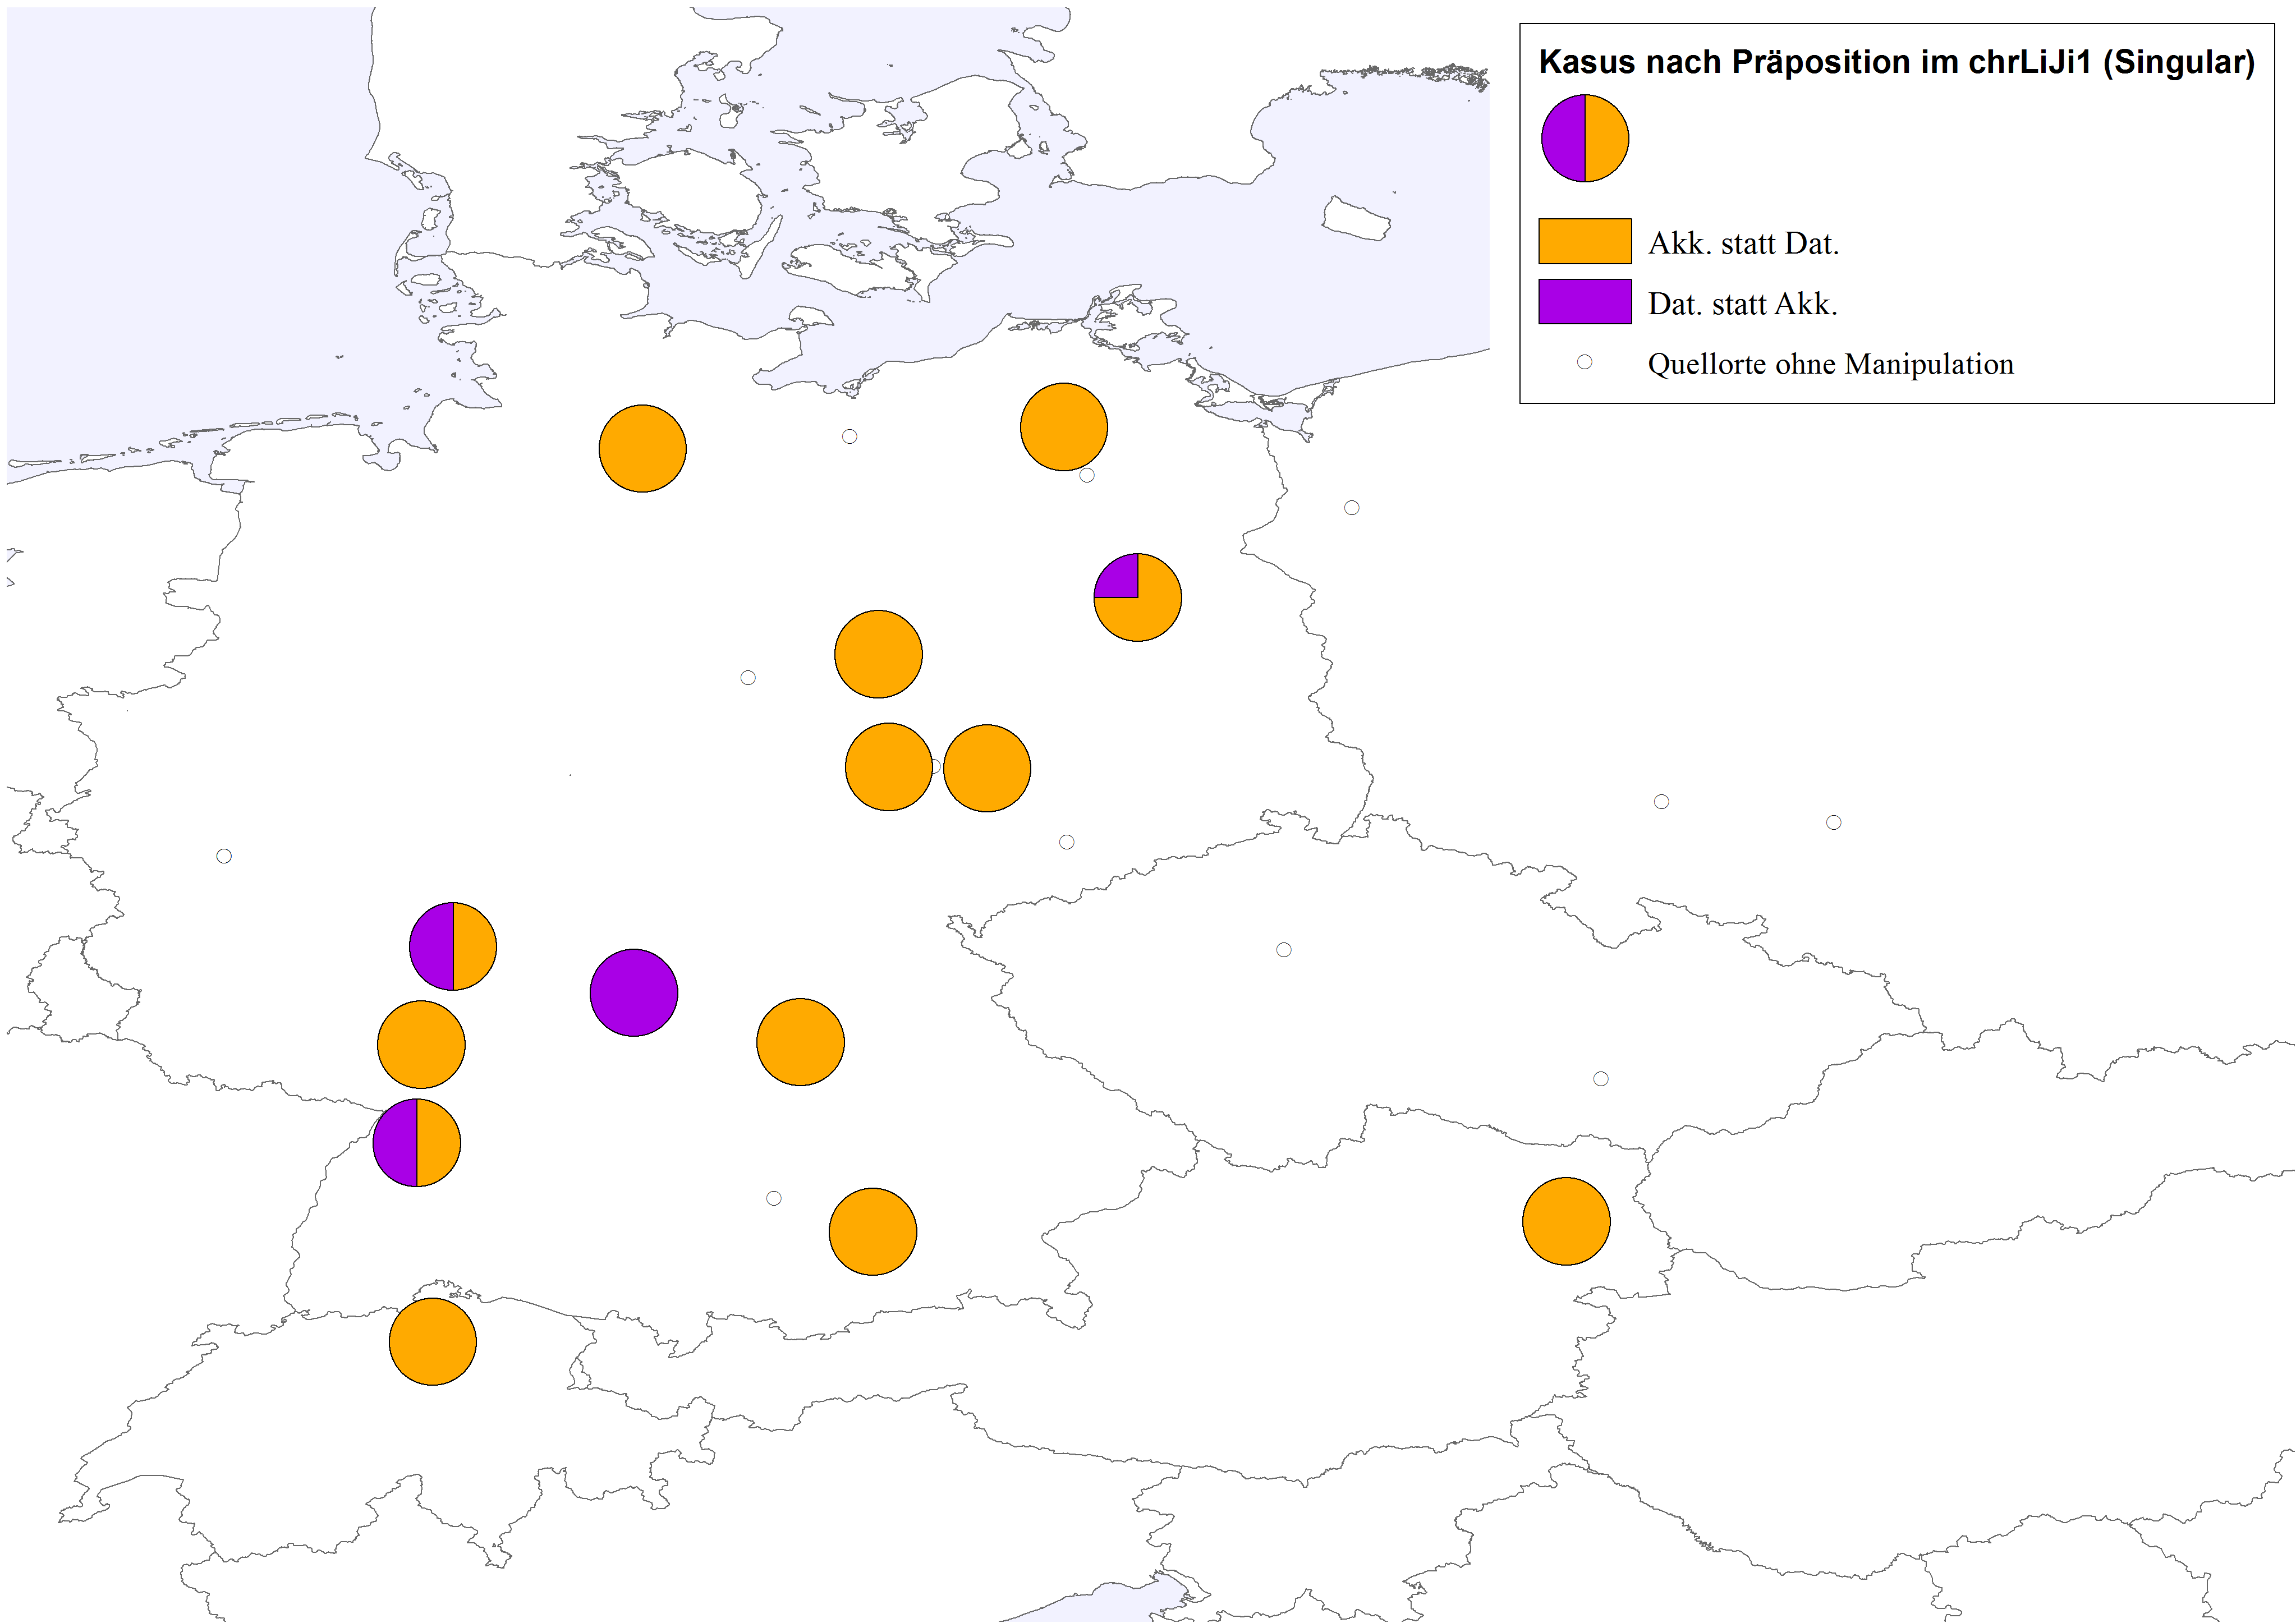
\includegraphics[width=\textwidth]{figures/KARTE_KASUS_PAEP_SG.png}
\caption{\label{kartepaepSG} Kasus nach \isi{Präposition} im \hai{chrLiJi1} (Singular)}
\end{figure}  
 
	



% \todo{Die nachfolgenden Tabellen und Grafiken nicht ins nächste Kapitel einrücken lassen!}

\begin{figure}[t] 
\fittable{
	\begin{tikzpicture}
		\begin{axis}[only marks, width=0.82\textwidth,height=0.2\textheight,
		legend style={at={(1,1)},xshift=+0.2cm, yshift=-0.0cm,anchor=north west,nodes=left},
			%title={Funktionstypen des sp\"aten Westjiddisch},
			xtick={1700, 1725, 1750, 1775, 1800, 1825, 1850, 1875, 1900, 1925, 1950, 1975}, ytick=\empty,
			x tick label style={/pgf/number format/1000 sep=}, 
			y tick label style={/pgf/number format/1000 sep=},
			%extra y ticks={456.1, 1022.4},
			%extra y tick labels={{456,1},{1022,4}},
			extra y tick style={grid=major,
				tick label style={, ,}},
				ymin=0.7,
				ymax=6.3,
				y=4.5mm,
			ylabel={Phänomenbelege},
			enlarge x limits=0.03]	
            
\addplot [mark=square*, black] table [x=jahr, y=PL_DAT] {figures/Kasus_Pron_PL_DAT.txt};	
	
\addplot [mark=square*, gray] table [x=jahr, y=PL_AKK] {figures/Kasus_Pron_PL_AKK.txt};			


\addplot [mark=*, black] table [x=jahr, y=DAT_statt_AKK] {figures/Kasus_Pron_DAT_statt_AKK.txt};


\addplot [mark=*, gray] table [x=jahr, y=AKK_statt_DAT] {figures/Kasus_Pron_AKK_statt_DAT.txt};



\addplot [mark=o,black] table [x=jahr, y=NO] {figures/Kasus_Pron_NO.txt};%1.5
 

						\legend{{\Dat} statt {\Akk} {\Pl}, {\Akk} statt {\Dat} {\Pl}, {\Dat} satt {\Akk} {\Sg}, {\Akk} statt {\Dat} {\Sg}, keine Manipulation} %macht Legende
		\end{axis}
	\end{tikzpicture}
}
	\caption{Verstöße gegen das schriftdeutsche Kasussystem im \hai{chrLiJi1} bei Präpositionalphrasen}
	\label{histokasusPP}	
\end{figure}




Die diachrone Verteilung der Belege des \hai{chrLiJi1} zeigt ein auffälliges Bild (s. Abbildung \ref{histokasusPP}): Markierungen am Kasus nach \isi{Präposition} treten, von wenigen Ausreißern abgesehen, ab den 1820er Jahren auf und finden sich ab diesem Zeitpunkt in beinahe jeder Quelle. Dabei sind Belege für den \isi{Dativ} im Singular, also die standardostjiddische und west-westjiddische Form eher in den Quellen des 20. Jahrhunderts anzutreffen. Hingegen tritt der \isi{Akkusativ} als Einheitskasus bereits in den frühesten Belegen (1778, 1802) einer Manipulation des Kasus nach \isi{Präposition} auf.

  

	\begin{figure}[t]
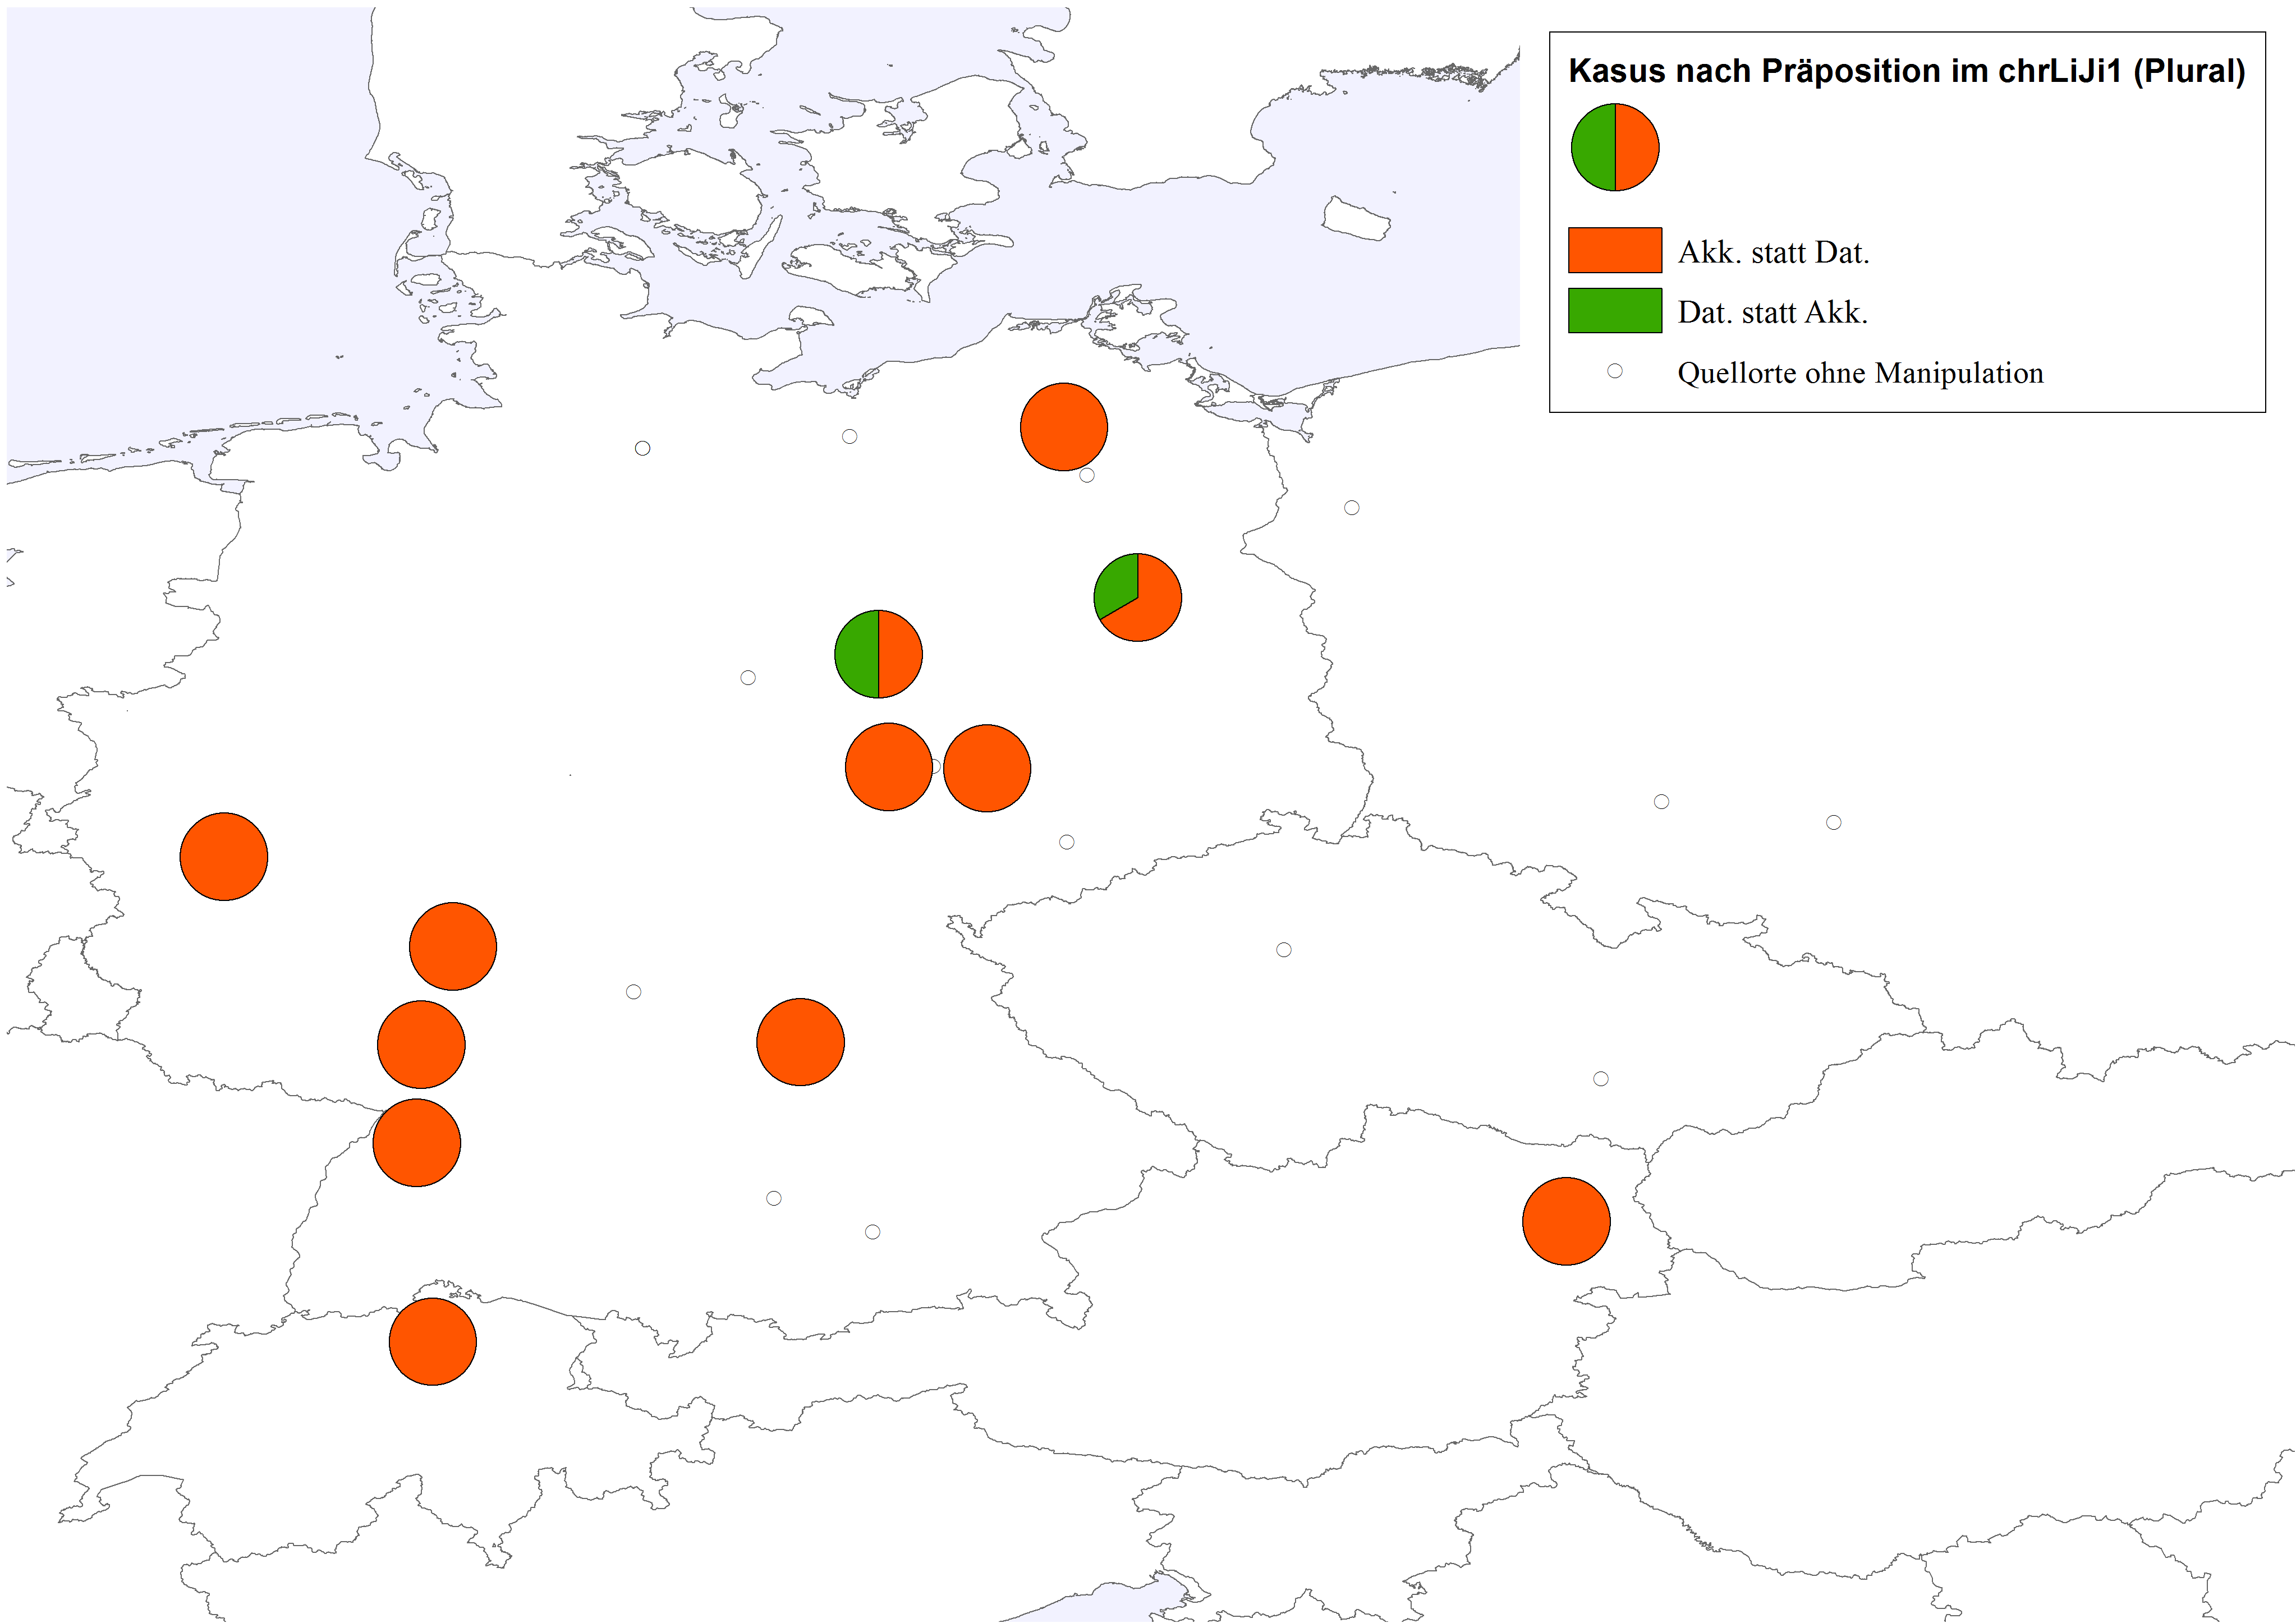
\includegraphics[width=\textwidth]{figures/KARTE_KASUS_PAEP_PL.png}
		\caption{\label{kartepaepPL} Kasus nach \isi{Präposition} im \hai{chrLiJi1} (Plural)}
		\end{figure}
  	 
  
      \subsection{Kasus bei Pronomen}\label{kasuspron}
 %  %\noindent
\largerpage[-1]
Das Pronominalsystem des Jiddischen fußt auf Lexemen der germanischen Komponente. Im Vergleich mit dem gegenwärtigen Schriftdeutschen stechen allerdings einige Synkretismen ins Auge. So sind im modernen Jiddisch die Personalpronomen der 3. Singular maskulin \isi{Akkusativ} und \isi{Dativ} zu \RL{ים} \textit{im} zusammengefallen (\citealt[115]{Wolf1969}; \citealt[185]{Jacobs2005}). In der 3. Plural ist der \isi{Dativ} mit der Form des Nominativs und Akkusativs \RL{זיי} \textit{zey} zusammengefallen. Desweiteren fand der \isi{Zusammenfall} von 1. Plural Nominativ und 1. Singular \isi{Dativ} zu \RL{מיר} \textit{mir} statt. Die Unterschiede zwischen Jiddisch und Deutsch sind bezüglich der Personalpronomina nicht sonderlich groß. Deutlich anders verhält sich modernes Standardjiddisch (und \hai{{\NOJ}}) beim Reflexivpronomen \RL{זיך} \textit{zikh}, welches nicht dekliniert wird. Darüber hinaus übernimmt dieses \isi{Pronomen} im Ostjiddischen syntaktische Funktionen, die dem deutschen Reflexivum nicht zukommen  und die höchst wahrscheinlich durch den Kontakt zu slawischen Sprachen begünstigt, wenn nicht sogar provoziert wurden (vgl.\, \citealt[185]{Jacobs2005}). Die pronominale Anredeform (Höflichkeitsform, \textit{T–V distinction}) wird im Jiddischen immer mittels der Form der 2. Person Plural \RL{איר} \textit{ir} gebildet. Darin unterscheidet es sich stark vom Deutschen, welches im Nominativ und \isi{Akkusativ} \textit{Sie} und im \isi{Dativ} \textit{Ihnen} verwendet. Die \isi{Pronomen} der Anredeform entsprechen hier also der 3. Person Plural.

Die Situation im Westjiddischen ist noch weitgehend unbeschrieben. In der zentralwestjiddischen Quelle \qu{Die Hochzeit zu Grobsdorf} findet sich ein Pronominalsystem mit deutlich stabiler Kasusdistinktion. Vom Schriftdeutschen abweichende Synkretismen können hier nur in der 3. Person Plural und beim Reflexivum festgestellt werden. Es findet sich die morphologische Form des Nominativs bzw. \isi{Akkusativ} \RL{זיע} \textit{sie} bei syntaktischem \isi{Dativ} (\ref{GrobSIE}). Wie im Ostjiddischen (und in den meisten hochdeutschen Dialekten) sind hier die Formen der 1. Person Plural Nominativ und der 1. Person Singular \isi{Dativ} unter \textit{mir} zusammengefallen (\ref{GrobMIR}–\ref{GrobSICH}). Weiterhin zeigt sich ein \isi{Synkretismus} beim Reflexivpronomen der 1. Plural \isi{Dativ}/\isi{Akkusativ} und der 3. Plural \isi{Dativ}/\isi{Akkusativ}  (\ref{GrobSICH}). Obwohl dieser \isi{Synkretismus} auch aus dem Ostjiddischen bekannt ist (s.\,o.), müssen die Belege aufgrund fehlender weiterer Evidenz in anderen westjiddischen Quellen aber eher auf Interferenzen mit dem zentralhessischen Dialekten zurückgeführt werden, für die dies ein typischer \isi{Zusammenfall} ist (\citealt[29]{Kehrein1860}). 


   \eenumsentence{
  
  \item {\RL{
וועממער בייא דיע הונד איס מוס מער מיט זיע גויטצע.}}\\
 \textit{wemmer bei die hund is mus mer mit sie gautze/goutze.}\\
  \sem{Wenn man bei den Hunden ist, muss man mit ihnen (wörtl. sie) bellen.} \\(\qu{Die Hochzeit zu Grobsdorf} 1822:\,76) \label{GrobSIE}
  

 \item {\RL{דערנויך ד{א\makebox(-1.25,-1.25)[r]{\libertineGlyph{uni05B7}}}נצע מיר וויררער.}}\\
 \textit{dernauch/dernouch danze mir wirrer.} \\
  \sem{Danach tanzen wir (wörtl. mir) wieder.} \\(\qu{Die Hochzeit zu Grobsdorf} 1822:\,85) \label{GrobMIR}
   
\newpage 
  
  \item {.\RL{מיר {{ג}\makebox(-0.5,-2.1)[r]{\libertineGlyph{uni05B5}}}יהן  אהַאם און {{ל}\makebox(-0.5,-2.1)[r]{\libertineGlyph{uni05B5}}}יעגע זיך בייא אונזער ווייבערכער}}\\
   \textit{mir geihn aham un leige sich bei unser weibercher.} \\
  \sem{Wir gehen heim und legen uns (wörtl. sich) zu unseren Frauen.} \\(\qu{Die Hochzeit zu Grobsdorf} 1822:\,85) \label{GrobSICH}
   
   }
   
   
   In den jiddischen Dialekten gibt es, soweit bekannt, keine starken Abweichungen vom Standard. Im \hai{{\NOJ}} sind \isi{Akkusativ} und \isi{Dativ} auch im Pronominalsystem zu einem obliquen Kasus zusammengefallen (s.\,o.). Bei den \isi{Pronomen} übernehmen die historischen Dativformen diesen Kasus (\citealt[184]{Jacobs2005}; \citealt[139–149]{Wolf1969}). Auch für das \hai{{\NÜJ}} ist ein \isi{Zusammenfall} der 1., 2. und 3. Person  Singular feminin der Personalpronomen von \isi{Dativ} und \isi{Akkusativ} zugunsten des Dativs z.\,T. belegt (vgl.\, \citealt[139–149]{Wolf1969}). Im \hai{{\NOJ}} und \hai{{\NÜJ}} ist also eine deutliche Profilierung des Dativs gegenüber dem \isi{Akkusativ} zu verzeichnen. Für das \hai{{\NWJ}} Aurichs stellt \cite[63]{Reershemius2007} ein unsicheres System der Personalpronomen im \isi{Akkusativ} und \isi{Dativ} der 1. und 2. Person Singular fest. Die ostjiddischen Synkretismen von 3. Person Singular maskulin \isi{Akkusativ} und \isi{Dativ} und von der 1. Person Plural Nominativ und 1. Person Singular \isi{Dativ} fanden hier jedoch nicht statt.  An weiteren Daten zum Westjiddischen fehlt es zur Zeit noch. 


Von sprachlichen Manipulation im Bereich der Pronominalmorphologie sind im \hai{{\LiJi}} ausschließlich Personal- und Reflexivpronomen betroffen. Insgesamt  zeigen 28 Quellen eine Manipulation des Kasus eines oder mehrerer \isi{Pronomen}. Pronomensynkretismen finden sich im \hai{{\LiJi}} besonders zwischen den Formen des Akkusativs und Dativs. Betroffen sind die 1., 2. und 3. Person  Singular maskulin der Personalpronomen (\ref{BSPDAT1})– (\ref{BSPAKK3}); aber auch die Homophonie von 1.  Person Plural Nominativ und  der 1. Person Singular \isi{Dativ} ist belegt (\ref{BSPmirPL}). Darüber hinaus spielten Abweichungen vom Schriftdeutschen bezüglich der Höflichkeitsform eine große Rolle im \hai{{\LiJi}}. Auch hier findet sich die Form des Nominativs/Akkusativs an der Position des Dativs (\ref{BSPNOMHoefl}) oder umgekehrt (\ref{BSPDATHoefl}). Nirgends aber wird die 2. Person Plural für die pronominale Anredeform verwendet, wie es für das Standard\-ostjiddische üblich wäre. Das sich besonders stark vom Deutschen absetzende ostjiddische System der Reflexivierung ist in keiner Quelle des \hai{{\LiJieins}} thematisiert. Reflexivpronomem sind zwar auch betroffen (\ref{BSPPRONREFLEXIV}), verhalten sich jedoch entsprechend dem Deutschen, wo sich das Reflexivum nur in der 3. Person von den Personalpronomen abhebt, in allen anderen Fällen aber lexikalisch identisch mit ihnen ist. 
 
   \eenumsentence{

 
 \item \textit{Taibche, Du kennst mir} (\hai{JP} Altona, 1867:\,12)\\
 \sem{Täubchen, du kennst mich}\label{BSPDAT1} 
  
  \item \textit{is mich ganz egal} (\hai{UT} Stavenhagen, 1862:\,Kap.\, 45)\\
   \sem{ist mir ganz egal}\label{BSPAKK1} 

  \item \textit{laß dir drücken an mein Herz} (\hai{AJ} Berlin, 1825:\,22)\\
   \sem{lass dich  drücken an mein Herz}\label{BSPDAT2} 

 \item \textit{Bleibet ich elahn bei dich zurück?} (\hai{IA} Erlangen, 1840:\,69)\\
 \sem{Bleibe ich allein bei dir zurück}\label{BSPAKK2} 
 
 \item \textit{hott en gewaltike Zurand genumme unn iss uff em gehuppft} (\hai{PG} Speyer, 1835:\,33)\\
 \sem{hat ihn gewaltig ran genommen und ist auf ihn  gehüpft}\label{BSPDAT3}
  
  \item \textit{hat er ihn gegeben ä Dachstübche fer umsonst} (\hai{SV} München, 1890:\,4)\\
   \sem{hat er ihm ein Dachstübchen für umsonst gegeben}\label{BSPAKK3} 
 
 \item \textit{Mir willen Scholem} (\hai{AK} Zürich, 1948:\,219)\\
  \sem{Wir  wollen Frieden}\label{BSPmirPL}

\item \textit{dorf ich Sie was rothen?} (\hai{AO} Wien, 1770:\,84)\\
\sem{darf ich Ihnen etwas raten?}\label{BSPDATHoefl}  

 \item \textit{ich liebe Ihnen} (\hai{AD} Leipzig, 1846:\,129, 137)\\
  \sem{ich liebe Sie } \label{BSPNOMHoefl}

\item \textit{Versteckel d'r unter e Decke} (\hai{VD} Frankfurt, 1916:\,17)\\
  \sem{verstecke dich  unter der Decke} \label{BSPPRONREFLEXIV}
 }
 
Belege, in denen das \isi{Pronomen} innerhalb einer \hai{{\PP}} steht und somit seinen syntaktischen Kasus von der \isi{Präposition} erhält, sind in den unten stehenden Tabellen (\ref{tblpronomenchrLiJi1} und \ref{tblpronomenjüdLiJi1}) 
durch eckige Klammern markiert. Nur selten, zumeist in der Höflichkeitsform, spielt die syntaktische Position jedoch eine Rolle für die Kasuswahl im \hai{{\LiJi}}.

 %einfügen Tabelle:tblpronomenchr\ili{LiJi1}
%format!  Problem bei Tabelle, unten funktioniert sie aber, und auch in der Einzeldatei tabelle.tex
 



 
 \begin{table}[p]
% \small
		\begin{tabularx}{\textwidth}{p{1cm}CCCCC}
		\lsptoprule 

\textbf{Quelle} &
{\textbf{1.\,{\Sg}}}  & 
{\textbf{2.\,{\Sg}}} &  
{\textbf{3.\,{\Sg}\,{\mask}}} &
{\textbf{1.\,{\Pl}\,{\Nom}}}  & 
{\textbf{Höfl.}}\\
 \midrule 

\hai{{\PP}} & \midgraycell%Dat. $\gets$ {\Akk} 
& \whitecell & \whitecell &  \whitecell & \whitecell \\  
\hai{BW} 
& \whitecell \textsubscript{{\bs}PP}%\midgraycell/\textsubscript{\hai{{\PP}}}%  Dat. $\gets$ {\Akk}
& \midgraycell% Dat. $\gets$ {\Akk}
              & \whitecell & \whitecell & \whitecell \\ 
% &  &  \midgraycellpp%[Dat. $\gets$ {\Akk}]\textsubscript{\hai{{\PP}}}
% & &  & \\
\hai{LS} 
&\midgraycell%  Dat. $\gets$ {\Akk} 
             & \whitecell & \whitecell &  \whitecell & \whitecell \\ 
\hai{BP} 
&\midgraycell%  Dat. $\gets$ {\Akk}
& & & & \midgraycell%Dat. $\gets$ {\Akk}
\\
\hai{FE} 
& \midgraycell%Dat. $\gets$ {\Akk}  
              & \whitecell & \whitecell &  \whitecell &  \whitecell \textsubscript{{\bs}PP}%\darkgraycell/\textsubscript{\hai{{\PP}}}%Nom./{\Akk} $\gets$ Dat.
\\ 
% & &  & & &\darkgraycell\textsubscript{\hai{{\PP}}}% [Nom./{\Akk} $\gets$ Dat.]\textsubscript{\hai{{\PP}}} 
 %\\ 
\hai{AO} 
& \lightgraycell%{\Akk} $\gets$ Dat. 
                & \whitecell & \whitecell &  \whitecell &  \whitecell \textsubscript{{\bs}PP}%\darkgraycell/\textsubscript{\hai{{\PP}}}%Nom./{\Akk} $\gets$ Dat.
\\ 
% & &  & & & \darkgraycell\textsubscript{\hai{{\PP}}}%[Nom./{\Akk} $\gets$ Dat.]\textsubscript{\hai{{\PP}}} 
 %\\ 
\hai{GP} 
& \whitecell & \whitecell &   \darkgraycellpp%[{\Akk} $\gets$ Dat.]\textsubscript{\hai{{\PP}}}
& \whitecell & \whitecell \\  
\hai{PG} 
& \darkgraycellpp%[{\Akk} $\gets$ Dat.]\textsubscript{\hai{{\PP}}}  
& \whitecell & \midgraycellpp% [Dat. $\gets$ {\Akk}]\textsubscript{\hai{{\PP}}}
 & \whitecell & \whitecell \\  
\hai{JK} 
& \whitecell &  \midgraycellpp%[Dat. $\gets$ {\Akk}]\textsubscript{\hai{{\PP}}} 
& \whitecell & \whitecell & \darkgraycell% Nom./{\Akk} $\gets$ Dat.
\\ 
\hai{TH} 
& \darkgraycell%{\Akk} $\gets$ Dat. 
               & \whitecell & \whitecell &  \whitecell & \whitecell \\  
\hai{AJ} 
& \midgraycell%Dat. $\gets$ {\Akk} 
              & \whitecell \textsubscript{{\bs}PP}%\midgraycell/\textsubscript{\hai{{\PP}}}%Dat. $\gets$ {\Akk} 
                               & \whitecell & \whitecell &  \darkgraycellpp%[Nom./{\Akk} $\gets$ Dat.]\textsubscript{\hai{{\PP}}}
\\ 
%& & \midgraycell\textsubscript{\hai{{\PP}}}%[Dat. $\gets$ {\Akk}]\textsubscript{\hai{{\PP}}} 
%& & & \\ 
\hai{DP}*
& \midgraycell%Dat. $\gets$ {\Akk}  
               & \whitecell & \whitecell &  \whitecell & \whitecell \\  
\hai{UT}* 
& \darkgraycell%{\Akk} $\gets$ Dat.  
               &\midgraycell% Dat. $\gets$ {\Akk}  
                            & \whitecell & \whitecell & \whitecell \\  
\hai{PA} 
& \whitecell \textsubscript{{\bs}PP}%\midgraycell/\textsubscript{\hai{{\PP}}}%Dat. $\gets$ {\Akk} 
                 &\midgraycell% Dat. $\gets$ {\Akk}  
                              & \whitecell & \whitecell &  \midgraycell%Dat. $\gets$ {\Akk}
\\ 
%& \midgraycell\textsubscript{\hai{{\PP}}}%[Dat. $\gets$ {\Akk}]\textsubscript{\hai{{\PP}}}
%& & & & \darkgraycell\textsubscript{\hai{{\PP}}}%[Nom./Akk. $\gets$ Dat.]\textsubscript{\hai{{\PP}}} %Ricarda hier PP anders als ohne
%\\ 
\hai{IA} 
&\darkgraycellpp% [Akk. $\gets$ Dat.]\textsubscript{\hai{{\PP}}}  
                &\darkgraycellpp% [Akk. $\gets$ Dat.]\textsubscript{\hai{{\PP}}}
                                & \whitecell & \whitecell & \whitecell \\  
\hai{FM} 
& \midgraycell%Dat. $\gets$ Akk. 
                & \whitecell & \whitecell &  \whitecell &  \darkgraycell%Nom./Akk. $\gets$ Dat.
\\ 
\hai{AB} 
& \midgraycell%Dat. $\gets$ Akk. 
                & \whitecell & \whitecell &  \whitecell &  \darkgraycell%Nom./Akk. $\gets$ Dat.
\\ 
\hai{JP} 
&\midgraycell% Dat. $\gets$ Akk. 
             &\midgraycell% Dat. $\gets$ Akk. 
                         & \whitecell &   \blackcell%1. {\Sg} Dat. 
                                                           &\midgraycell% Dat. $\gets$ Akk.
 \\ 
\hai{SS} 
& \midgraycell%Dat. $\gets$ Akk. 
             & \whitecell & \whitecell &  \whitecell & \whitecell \\  
\hai{FL} 
& \whitecell & \whitecell &  \whitecell &   \blackcell%1. {\Sg} Dat.  
                                                             & \whitecell \\  
\hai{LP} 
& \whitecell & \whitecell &  \whitecell & \whitecell &  \midgraycell%Dat. $\gets$ Akk.
\\ 
\hai{VD} 
&\midgraycell% Dat. $\gets$ Akk. 
              & \midgraycell%Dat. $\gets$ Akk.  
                            & \whitecell & \whitecell & \whitecell \\  
\hai{AD} 
& \midgraycell% Dat. $\gets$ Akk.
              & \midgraycell%Dat. $\gets$ Akk.  
                            & \whitecell & \whitecell & \whitecell \textsubscript{{\bs}PP}%\midgraycell%Dat. $\gets$ Akk.;
 \\
%& & & & & \darkgraycell\textsubscript{\hai{{\PP}}}%[Nom./Akk. $\gets$ Dat.]\textsubscript{\hai{{\PP}}}
%\\  %Ricarda hier PP anders als ohne
\hai{MV} 
& \midgraycell% Dat. $\gets$ Akk. 
              & \whitecell & \whitecell &  \whitecell & \darkgraycellpp% [Nom./Akk. $\gets$ Dat.]\textsubscript{\hai{{\PP}}}
\\ 
\hai{DG} 
&\midgraycellpp% [Dat. $\gets$ Akk.]\textsubscript{\hai{{\PP}}}
               & \whitecell & \whitecell &  \whitecell & \whitecell \\  
\hai{GW} 
& \whitecell & \whitecell &  \whitecell &  \blackcell% 1. {\Sg} Dat.  
                                                            & \midgraycell%Dat. $\gets$ Akk.
\\ 
\hai{SV} 
& \midgraycell%Dat. $\gets$ Akk.
              & \whitecell &  \darkgraycell%Akk. $\gets$ Dat. 
                                           & \blackcell% 1. {\Sg} Dat.  
                                                              & \whitecell \\  
\hai{AK} 
& \whitecell & \whitecell &  \whitecell &  \blackcell% 1. {\Sg} Dat. 
                                                            & \whitecell \\ 
\midrule 

\midgraycell  & \multicolumn{5}{l}{\footnotesize{= {\Dat} statt {\Akk}}} \\
\darkgraycell & \multicolumn{5}{l}{\footnotesize{= {\Akk} statt {\Dat}}} \\
\blackcell    & \multicolumn{5}{l}{\footnotesize{= 1. {\Sg} {\Dat}}}  \\ 

\midrule 
   
\scriptsize{\hai{{\bs}PP}} & \multicolumn{5}{l}{neben Belegen mit \isi{Pronomen} nach Präposition}\\
\scriptsize{\hai{{\PP}}}  & \multicolumn{5}{l}{ausschließlich Belege mit \isi{Pronomen} nach Präposition}\\

\lspbottomrule
  \end{tabularx}
		 \caption{Kasussynkretismen bei Personalpronomen im \hai{chrLiJi1}.
%\todo[inline]{Ich habe versuct die tabelle zu vereinfachen; ohne Erfolg}
} 		 \label{tblpronomenchrLiJi1}


 
%\begin{tikzpicture}[remember picture,overlay]
%\path[fill=white,opacity=0.2](a.north west)--(a.south west) -- (a.south east) -- cycle;
%\path[fill=gray,opacity=0.3](a.north east)--(a.south east) -- (a.north west) -- cycle;
%
%\path[fill=white,opacity=0.2](b.north west)--(b.south west) -- (b.south east) -- cycle;
%\path[fill=gray,opacity=0.3](b.north east)--(b.south east) -- (b.north west) -- cycle;
%
%\path[fill=white,opacity=0.2](c.north west)--(c.south west) -- (c.south east) -- cycle;
%\path[fill=gray,opacity=0.3](c.north east)--(c.south east) -- (c.north west) -- cycle;
%
%
%\path[fill=white,opacity=0.2](d.north west)--(d.south west) -- (d.south east) -- cycle;
%\path[fill=gray,opacity=0.95](d.north east)--(d.south east) -- (d.north west) -- cycle;
%
%\path[fill=white,opacity=0.2](e.north west)--(e.south west) -- (e.south east) -- cycle;
%\path[fill=gray,opacity=0.95](e.north east)--(e.south east) -- (e.north west) -- cycle;
%
%\path[fill=gray,opacity=0.3](e2.north west)--(e2.south west) -- (e2.south east) -- cycle;
%\path[fill=gray,opacity=0.95](e2.north east)--(e2.south east) -- (e2.north west) -- cycle;
%\end{tikzpicture}
          

		 \end{table}

     % einfügen Tabelle tblpronomenjüd\ili{LiJi1}
     	 \begin{table} 

%\begin{longtable}{ccc|ccc}

		\begin{tabular}{lccccc}
		\lsptoprule 

\textbf{Quelle} &\textbf{1. {\Sg}}  & \textbf{2. {\Sg}} &  \textbf{3. {\Sg} {\mask}} &\textbf{1. {\Pl} {\Nom}}  & \textbf{Höfl.}\\ \midrule 

\hai{GuS1} & \whitecellpp{f}%\midgraycell%Dat. $\gets$ Akk. 
& \whitecell &  –& 
\blackcell%1. {\Sg} Dat.  
& –\\  
% & \midgraycell\textsubscript{\hai{{\PP}}}%[Dat. $\gets$ Akk.]\textsubscript{\hai{{\PP}}} 
% & && & \\
\hai{GuS5} & \midgraycell%Dat. $\gets$ Akk. 
& \whitecell &  –& \blackcell%1. {\Sg} Dat.
& –\\
\hai{GuS10} & \whitecellpp{g}%\midgraycell%Dat. $\gets$ Akk.  
& \midgraycell%Dat. $\gets$ Akk.  
& \whitecell &  –&  \darkgraycell%Nom./Akk. $\gets$ Dat.
\\
% & \midgraycell\textsubscript{\hai{{\PP}}}%[Dat. $\gets$ Akk.]\textsubscript{\hai{{\PP}}} 
% & && & \\
\hai{GuS15} & \midgraycell%Dat. $\gets$ Akk. 
& \whitecell &  –& \whitecell &   \darkgraycell%Nom./Akk. $\gets$ Dat.
\\
\hai{GuS23} & \midgraycell%Dat. $\gets$ Akk. 
& \whitecell &  \midgraycell%Dat. $\gets$ Akk.
& \whitecell &  \midgraycell%Dat. $\gets$ Akk.
\\
\hai{PAlsleben} & \midgraycell%Dat. $\gets$ Akk. 
& \whitecell &  –& \whitecell &  –\\
\hai{PBreslau} & \midgraycell%Dat. $\gets$ Akk.  
& \midgraycell%Dat. $\gets$ Akk.  
& \whitecell &  –& –\\
\hai{PBerlin1} & \whitecell &  – & \whitecell &  –&  \darkgraycell%Nom./Akk. $\gets$ Dat.
\\
\hai{PBerlin2} & \whitecell &  – & \whitecell &  \blackcell%1. {\Sg} Dat. 
& –\\
\midrule 
\midgraycell & \multicolumn{2}{l}{\footnotesize{= {\Dat} statt {\Akk}}} &
\darkgraycell & \multicolumn{2}{l}{\footnotesize{= {\Akk} statt {\Dat}}} \\
\blackcell & \multicolumn{5}{l}{\footnotesize{= 1. {\Sg} {\Dat}}}  \\ %\midrule 

\lspbottomrule
 \end{tabular}
		 \caption{Kasussynkretismen bei Personalpronomen im \hai{jüdLiJi1}}
		 \label{tblpronomenjüdLiJi1}
		 \end{table}

\begin{tikzpicture}[remember picture,overlay]
% \path[fill=white,opacity=0.2](f.north west)--(f.south west) -- (f.south east) -- cycle;
% \path[fill=gray,opacity=0.3](f.north east)--(f.south east) -- (f.north west) -- cycle;
% 
% \path[fill=white,opacity=0.2](g.north west)--(g.south west) -- (g.south east) -- cycle;
% \path[fill=gray,opacity=0.3](g.north east)--(g.south east) -- (g.north west) -- cycle;


\end{tikzpicture} 


 
 
 
23 Quellen des \hai{chrLiJi1} zeigen Wechsel der Akkusativ- und Dativformen in der 1. Person Singular. Die Dativform wird in 16 (18 inkl. \hai{{\PP}}) Fällen an der Position des Akkusativs gesetzt. Das Akkusativpronomen anstelle des Dativs findet sich in drei (5 inkl. \hai{{\PP}}) Quellen. In der 1. Person Singular profiliert damit deutlich der \isi{Dativ} über den \isi{Akkusativ}. 
 Ein ähnliches Bild zeigt sich bei der 2. Person Singular. Der \isi{Dativ} statt \isi{Akkusativ} findet sich in sieben (10 inkl. \hai{{\PP}}) Quellen; der \isi{Akkusativ} anstelle des Dativs hingegen in nur einem Beleg nach \isi{Präposition}.
 Die 3. Person Singular maskulin ist am seltensten von Manipulationen betroffen. Hier überwiegt der \isi{Akkusativ} leicht gegenüber dem \isi{Dativ}. Zwei Quellen (inkl. \hai{{\PP}}) zeigen den \isi{Akkusativ} statt des Dativs. Nur ein Beleg nach \isi{Präposition} zeigt die Dativform anstelle des Akkusativs. 
 Die Homophonie von der 1. Person Plural Nominativ und der 1. Person Singular \isi{Dativ} wird von fünf Texten des \hai{chrLiJi1} umgesetzt.
 Die Höflichkeitsform wird in 13 Quellen manipuliert; sechs Quellen setzen die Form des Dativs anstelle des Akkusativs. Fünf Quellen zeigen die Form des Nominativs/Akkusativs anstelle des Dativs. Sieben Quellen, einschließlich der sechs Quellen mit der Verwendung von Nominativ-/Akkusativform  anstelle des Dativs bei \hai{{\PP}}. 


 
 
 
 
 
 
 

 
Die nachfolgenden Karten (Abbildung \ref{kartePRON1}, \ref{kartePRON2}, \ref{kartePRON3}, \ref{kartePRON4}) und das Diagramm in Abbildung \ref{histokasusPRONOMEN} stellen nur die Daten für \isi{Pronomen} in vollen \hai{{\NP}}s dar. Die Belege für \isi{Pronomen} nach Präpositionen werden nicht weiter berücksichtigt, da sie die Stichprobe verfälschen würden.

 	\begin{figure} 

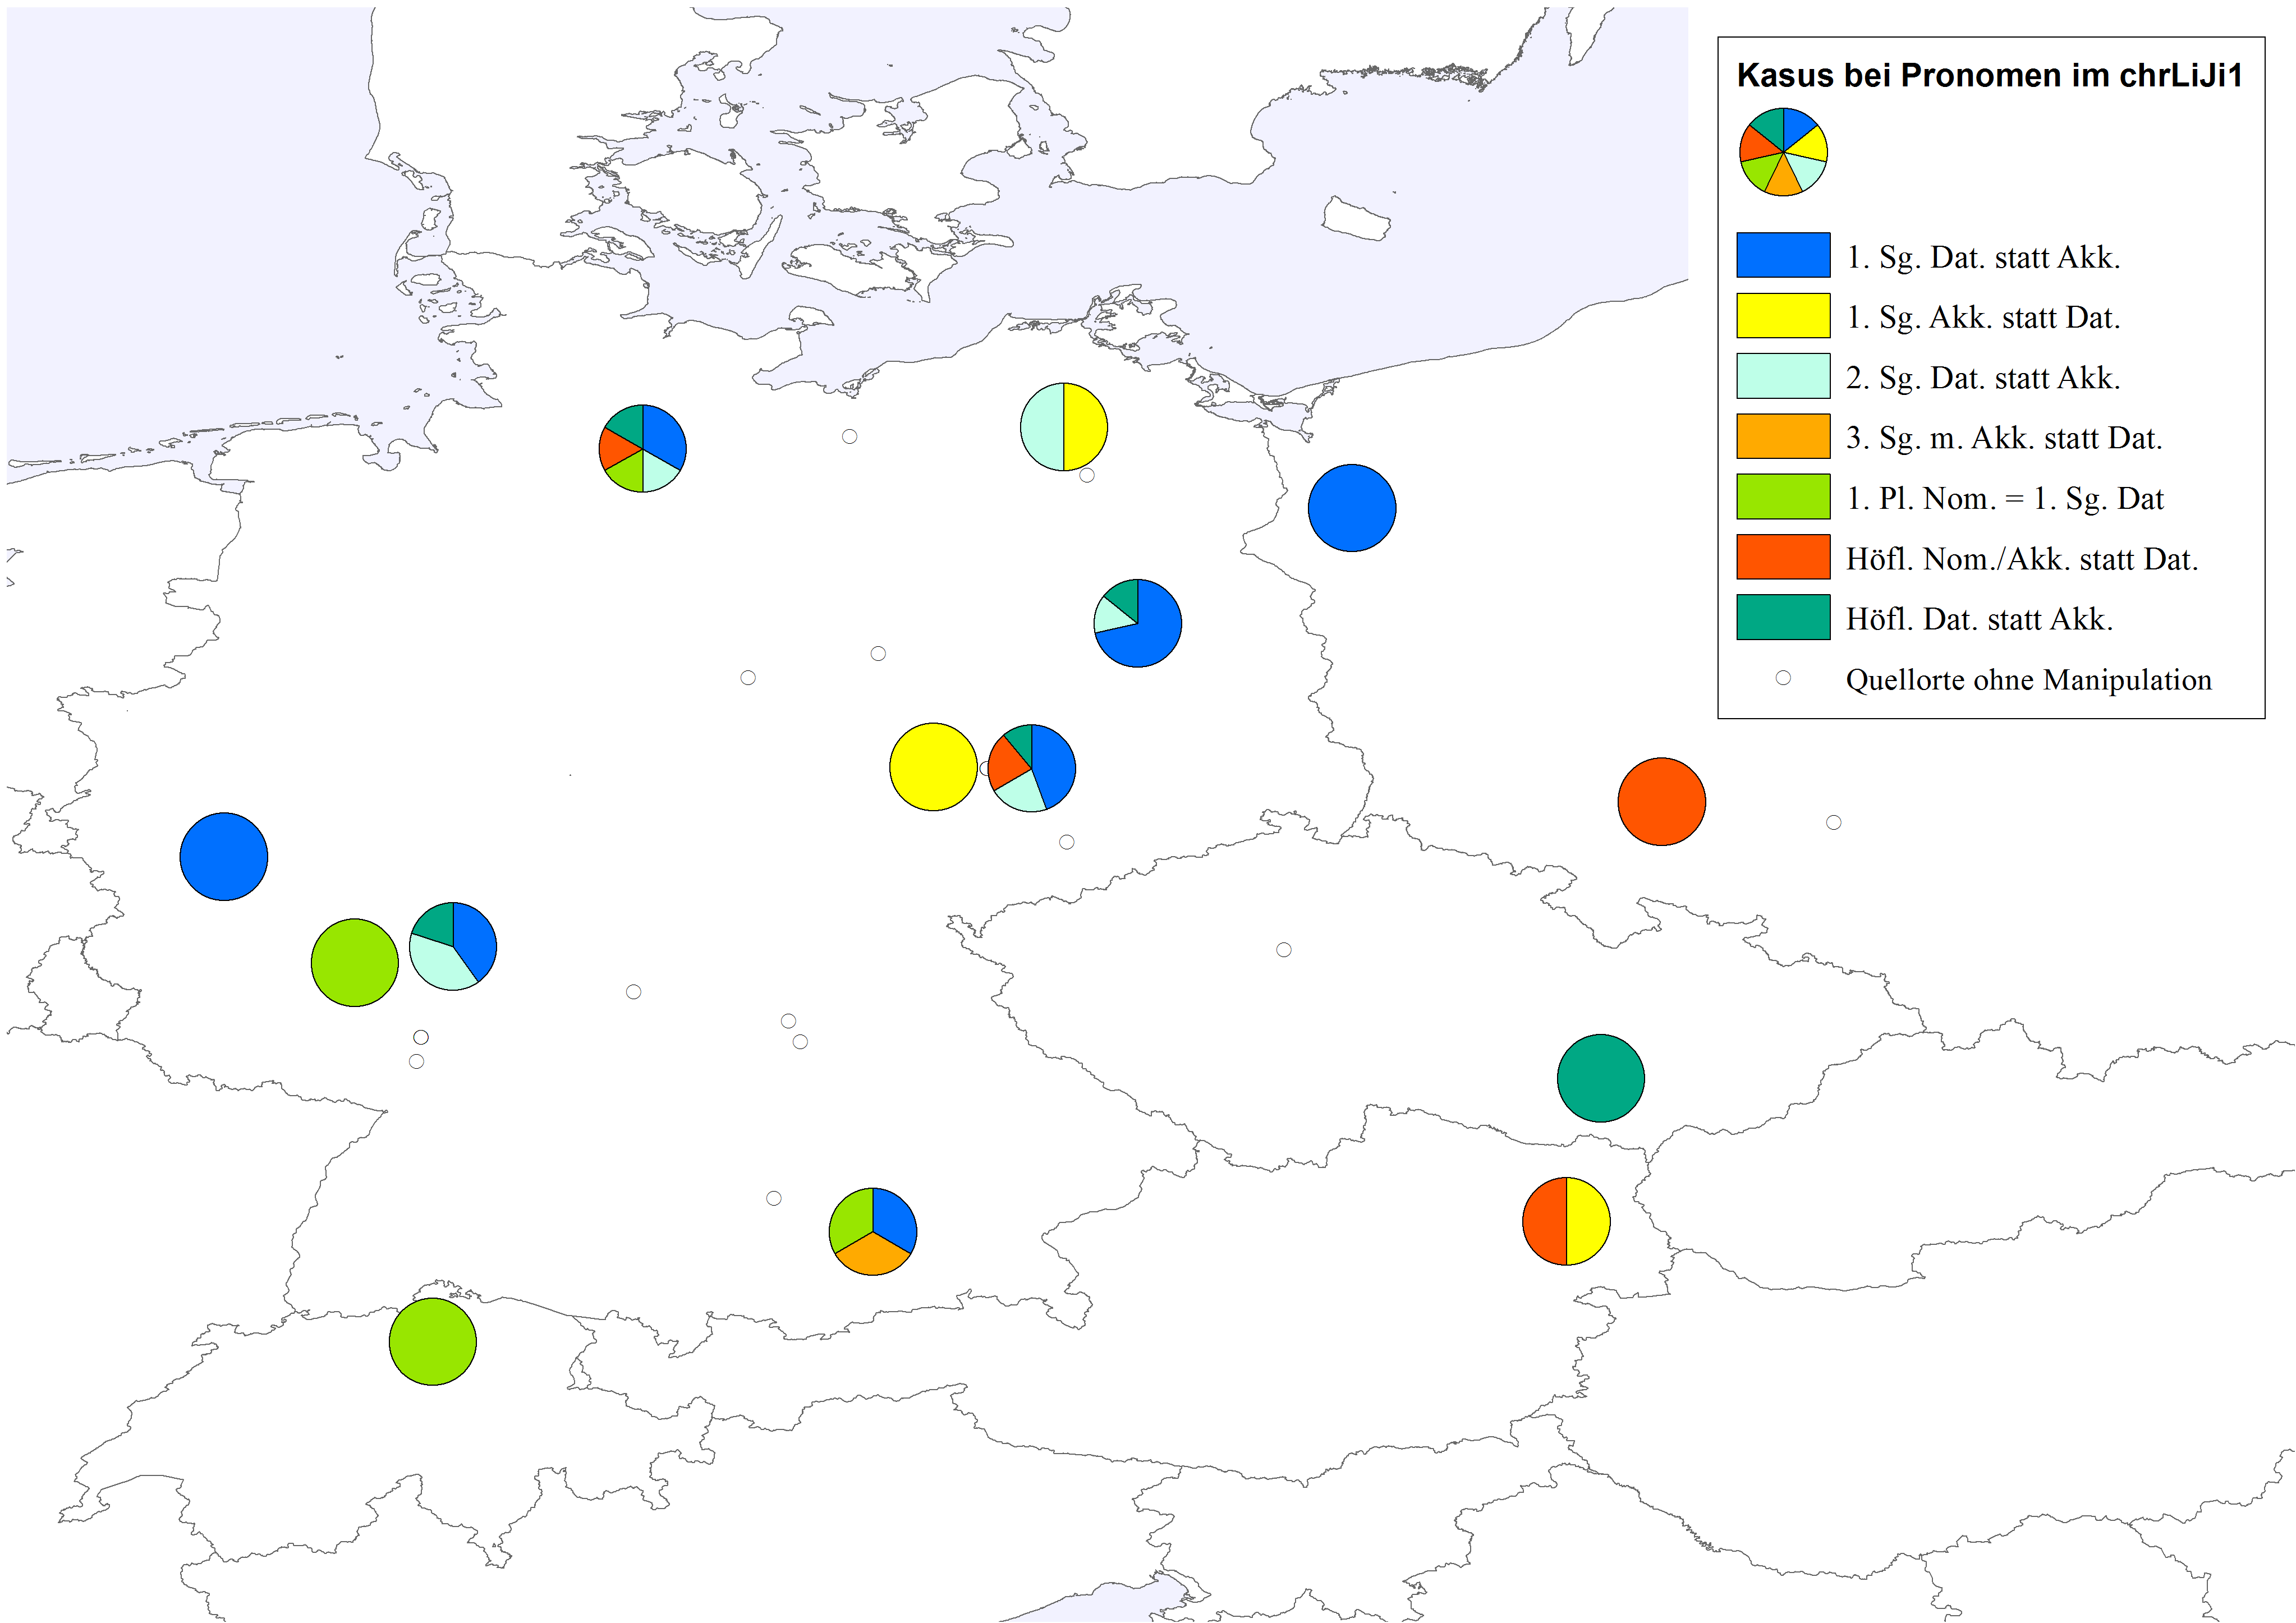
\includegraphics[height=.4\textheight]{figures/PRONOMEN_ALLE_Karte.png}
		\caption{\label{kartePRON1} Kasusmarkierung an Personalpronomen im \hai{chrLiJi1}}
		\end{figure}
  %farbe des meeres neu / heller!!!
		
	
	\begin{figure} 

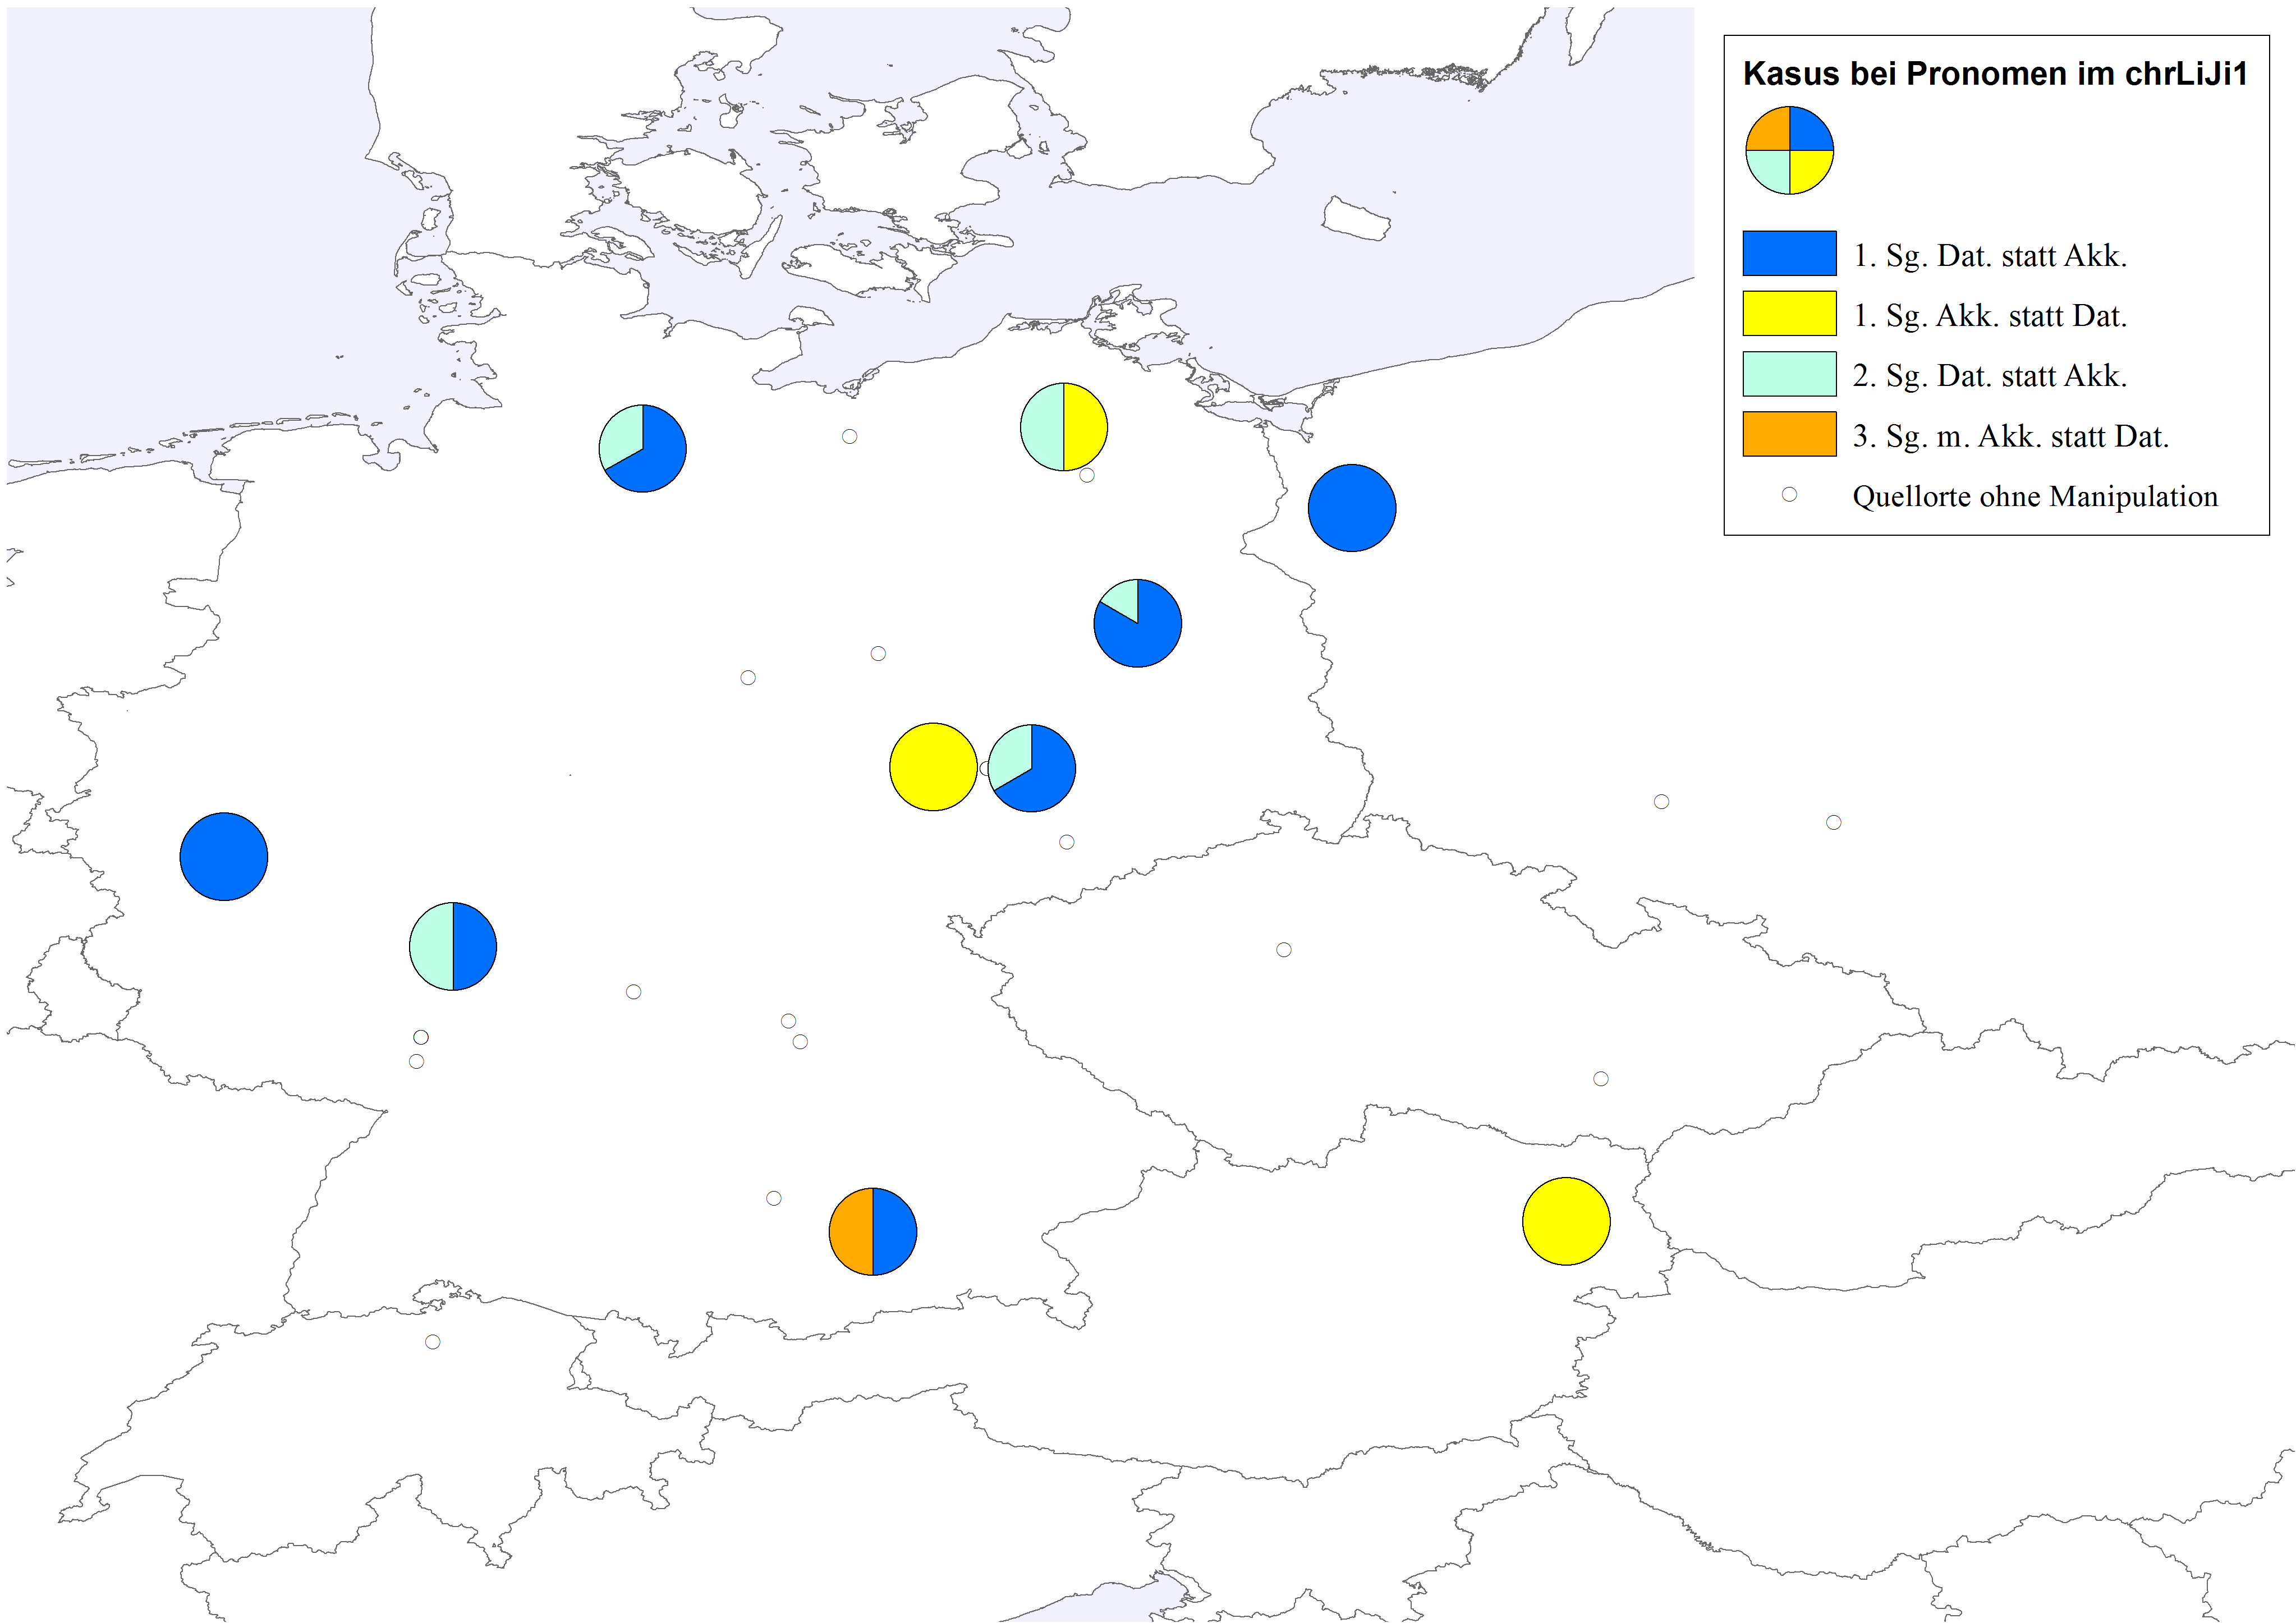
\includegraphics[height=.4\textheight]{figures/PRONOMEN_KARTE_allesSG.png}
		\caption{\label{kartePRON2} Kasusmarkierung von {\Akk}/{\Dat} an Personalpronomen im {\Sg}}
		\end{figure}
  %farbe des meeres neu / heller!!!
		

	
\begin{figure} 

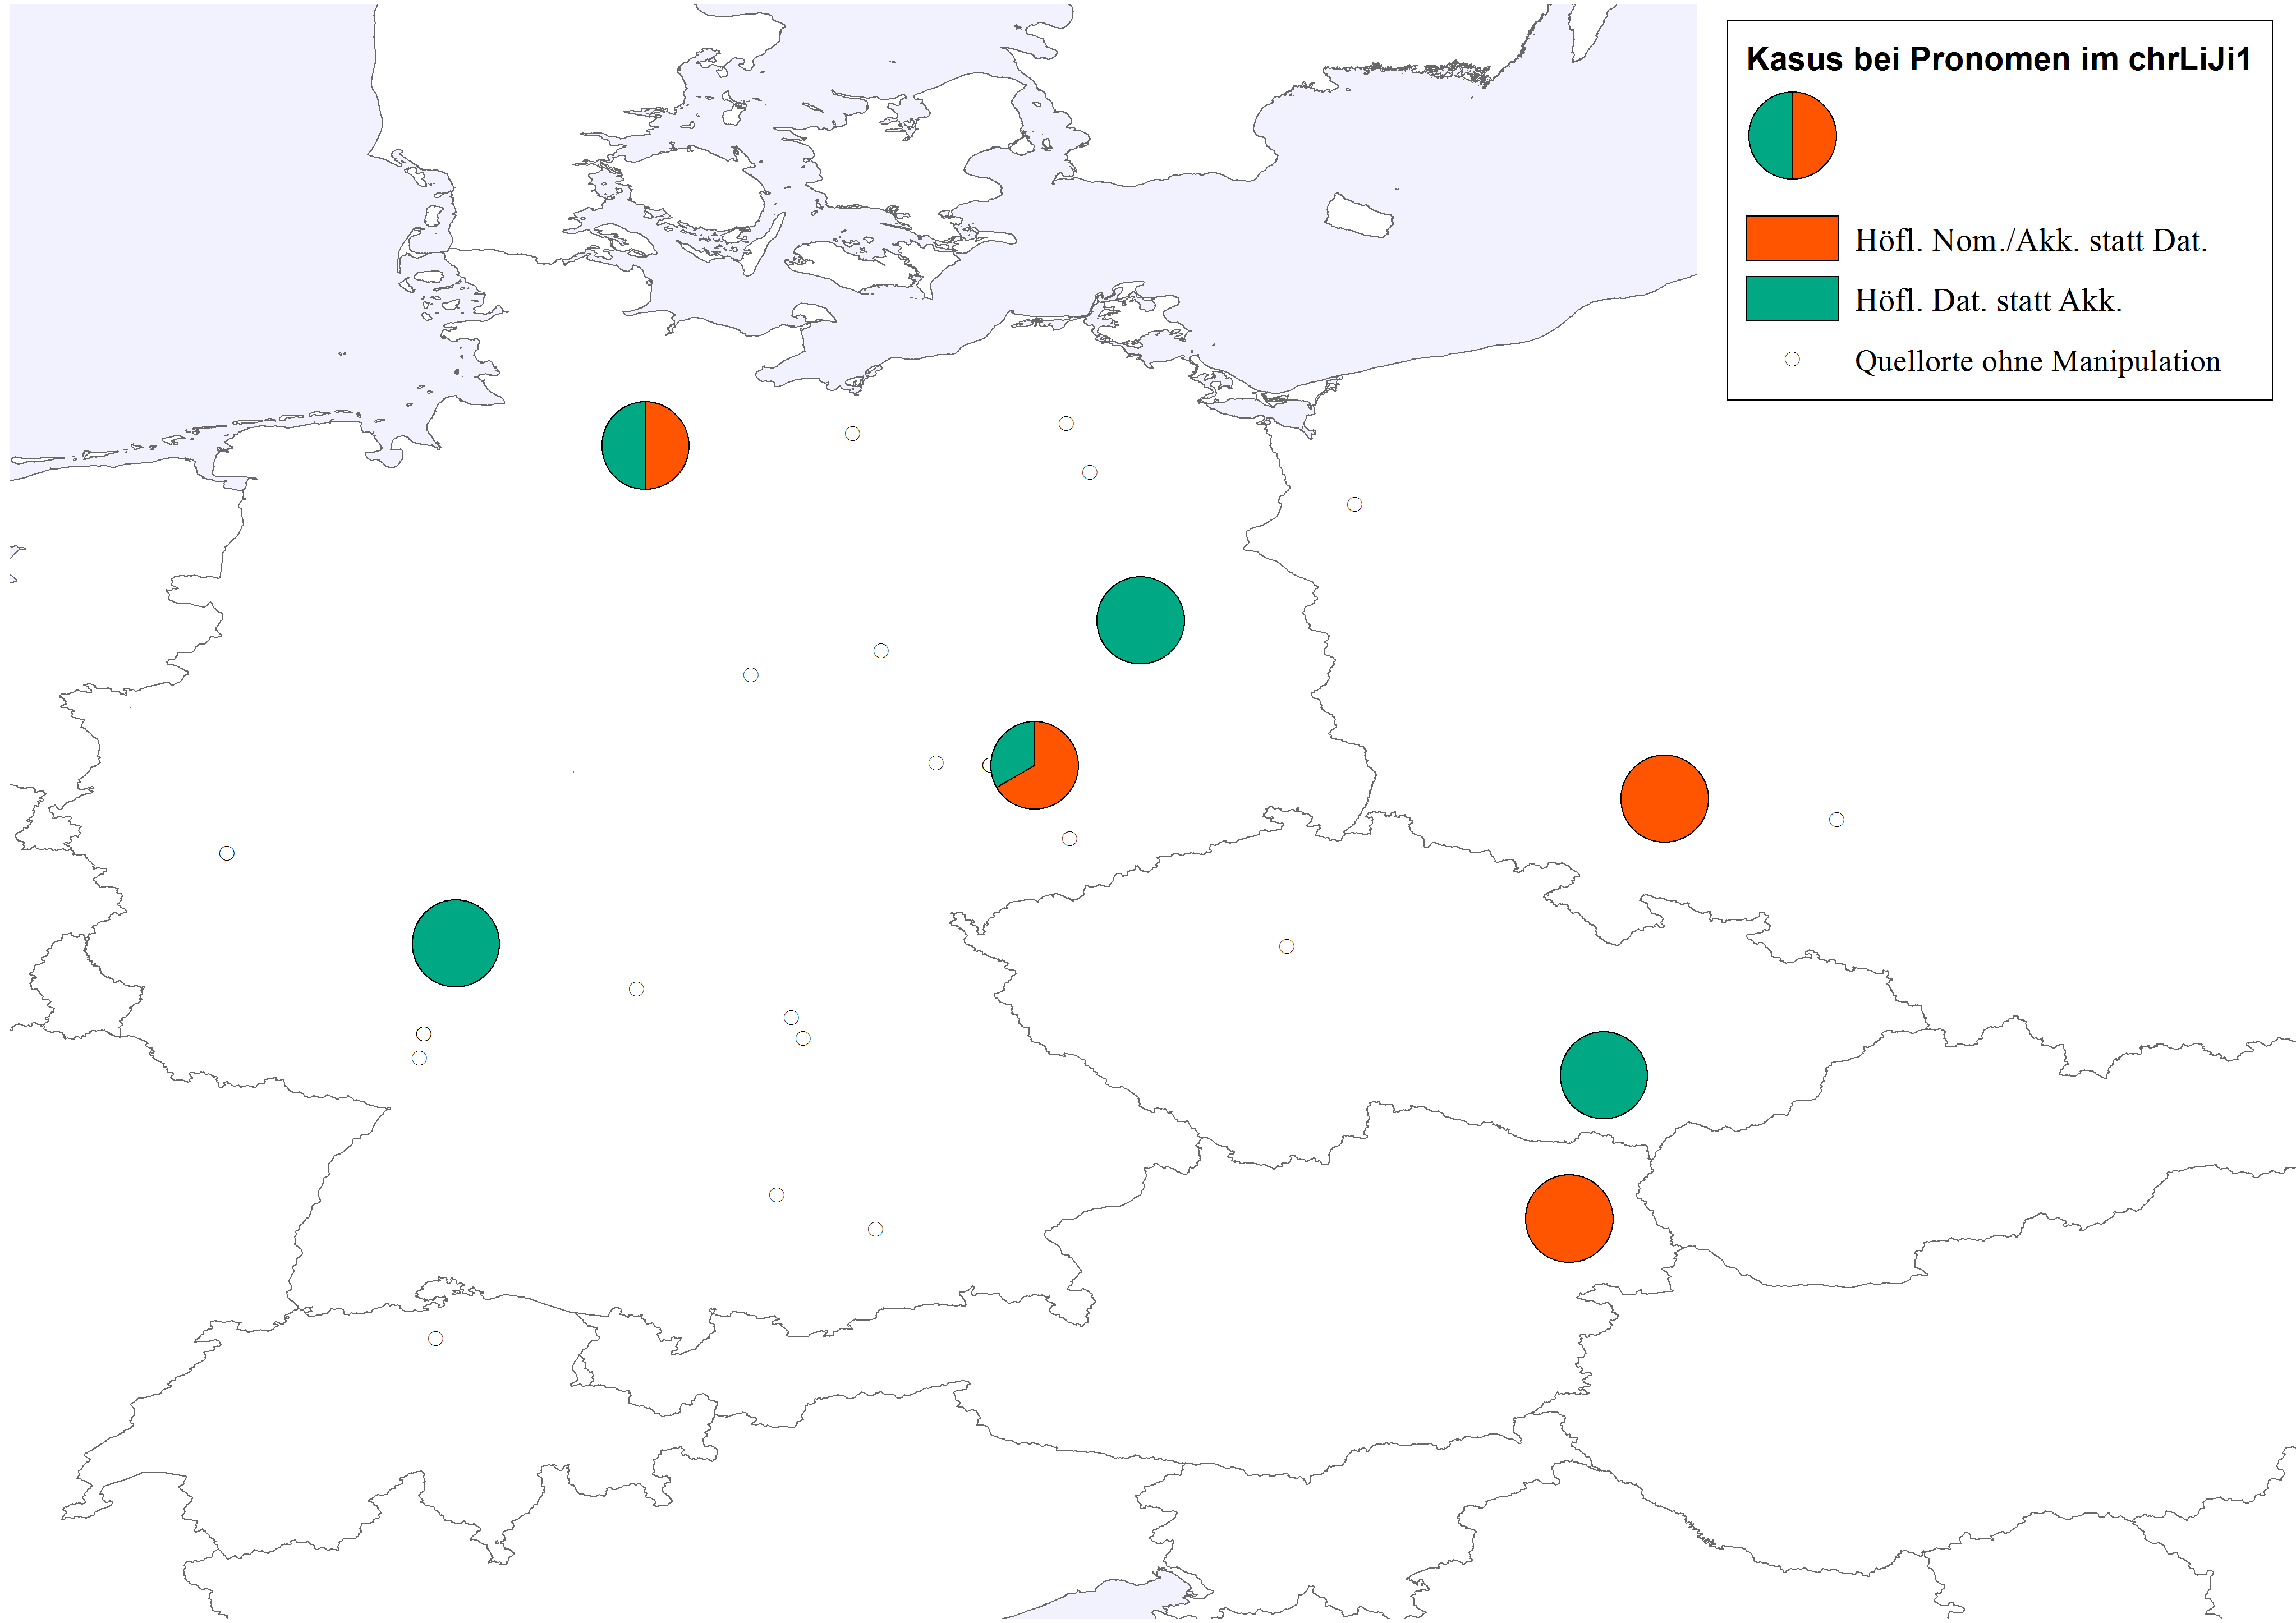
\includegraphics[height=.4\textheight]{figures/PRONOMEN_HOEFLICHKEITSFORMEN.png}
		\caption{\label{kartePRON3} Kasusmarkierung von {\Nom},{\Akk}/{\Dat} an Personalpronomen der Höflichkeitsform}
		\end{figure}
  %farbe des meeres neu / heller!!!
		
  

\begin{figure} 

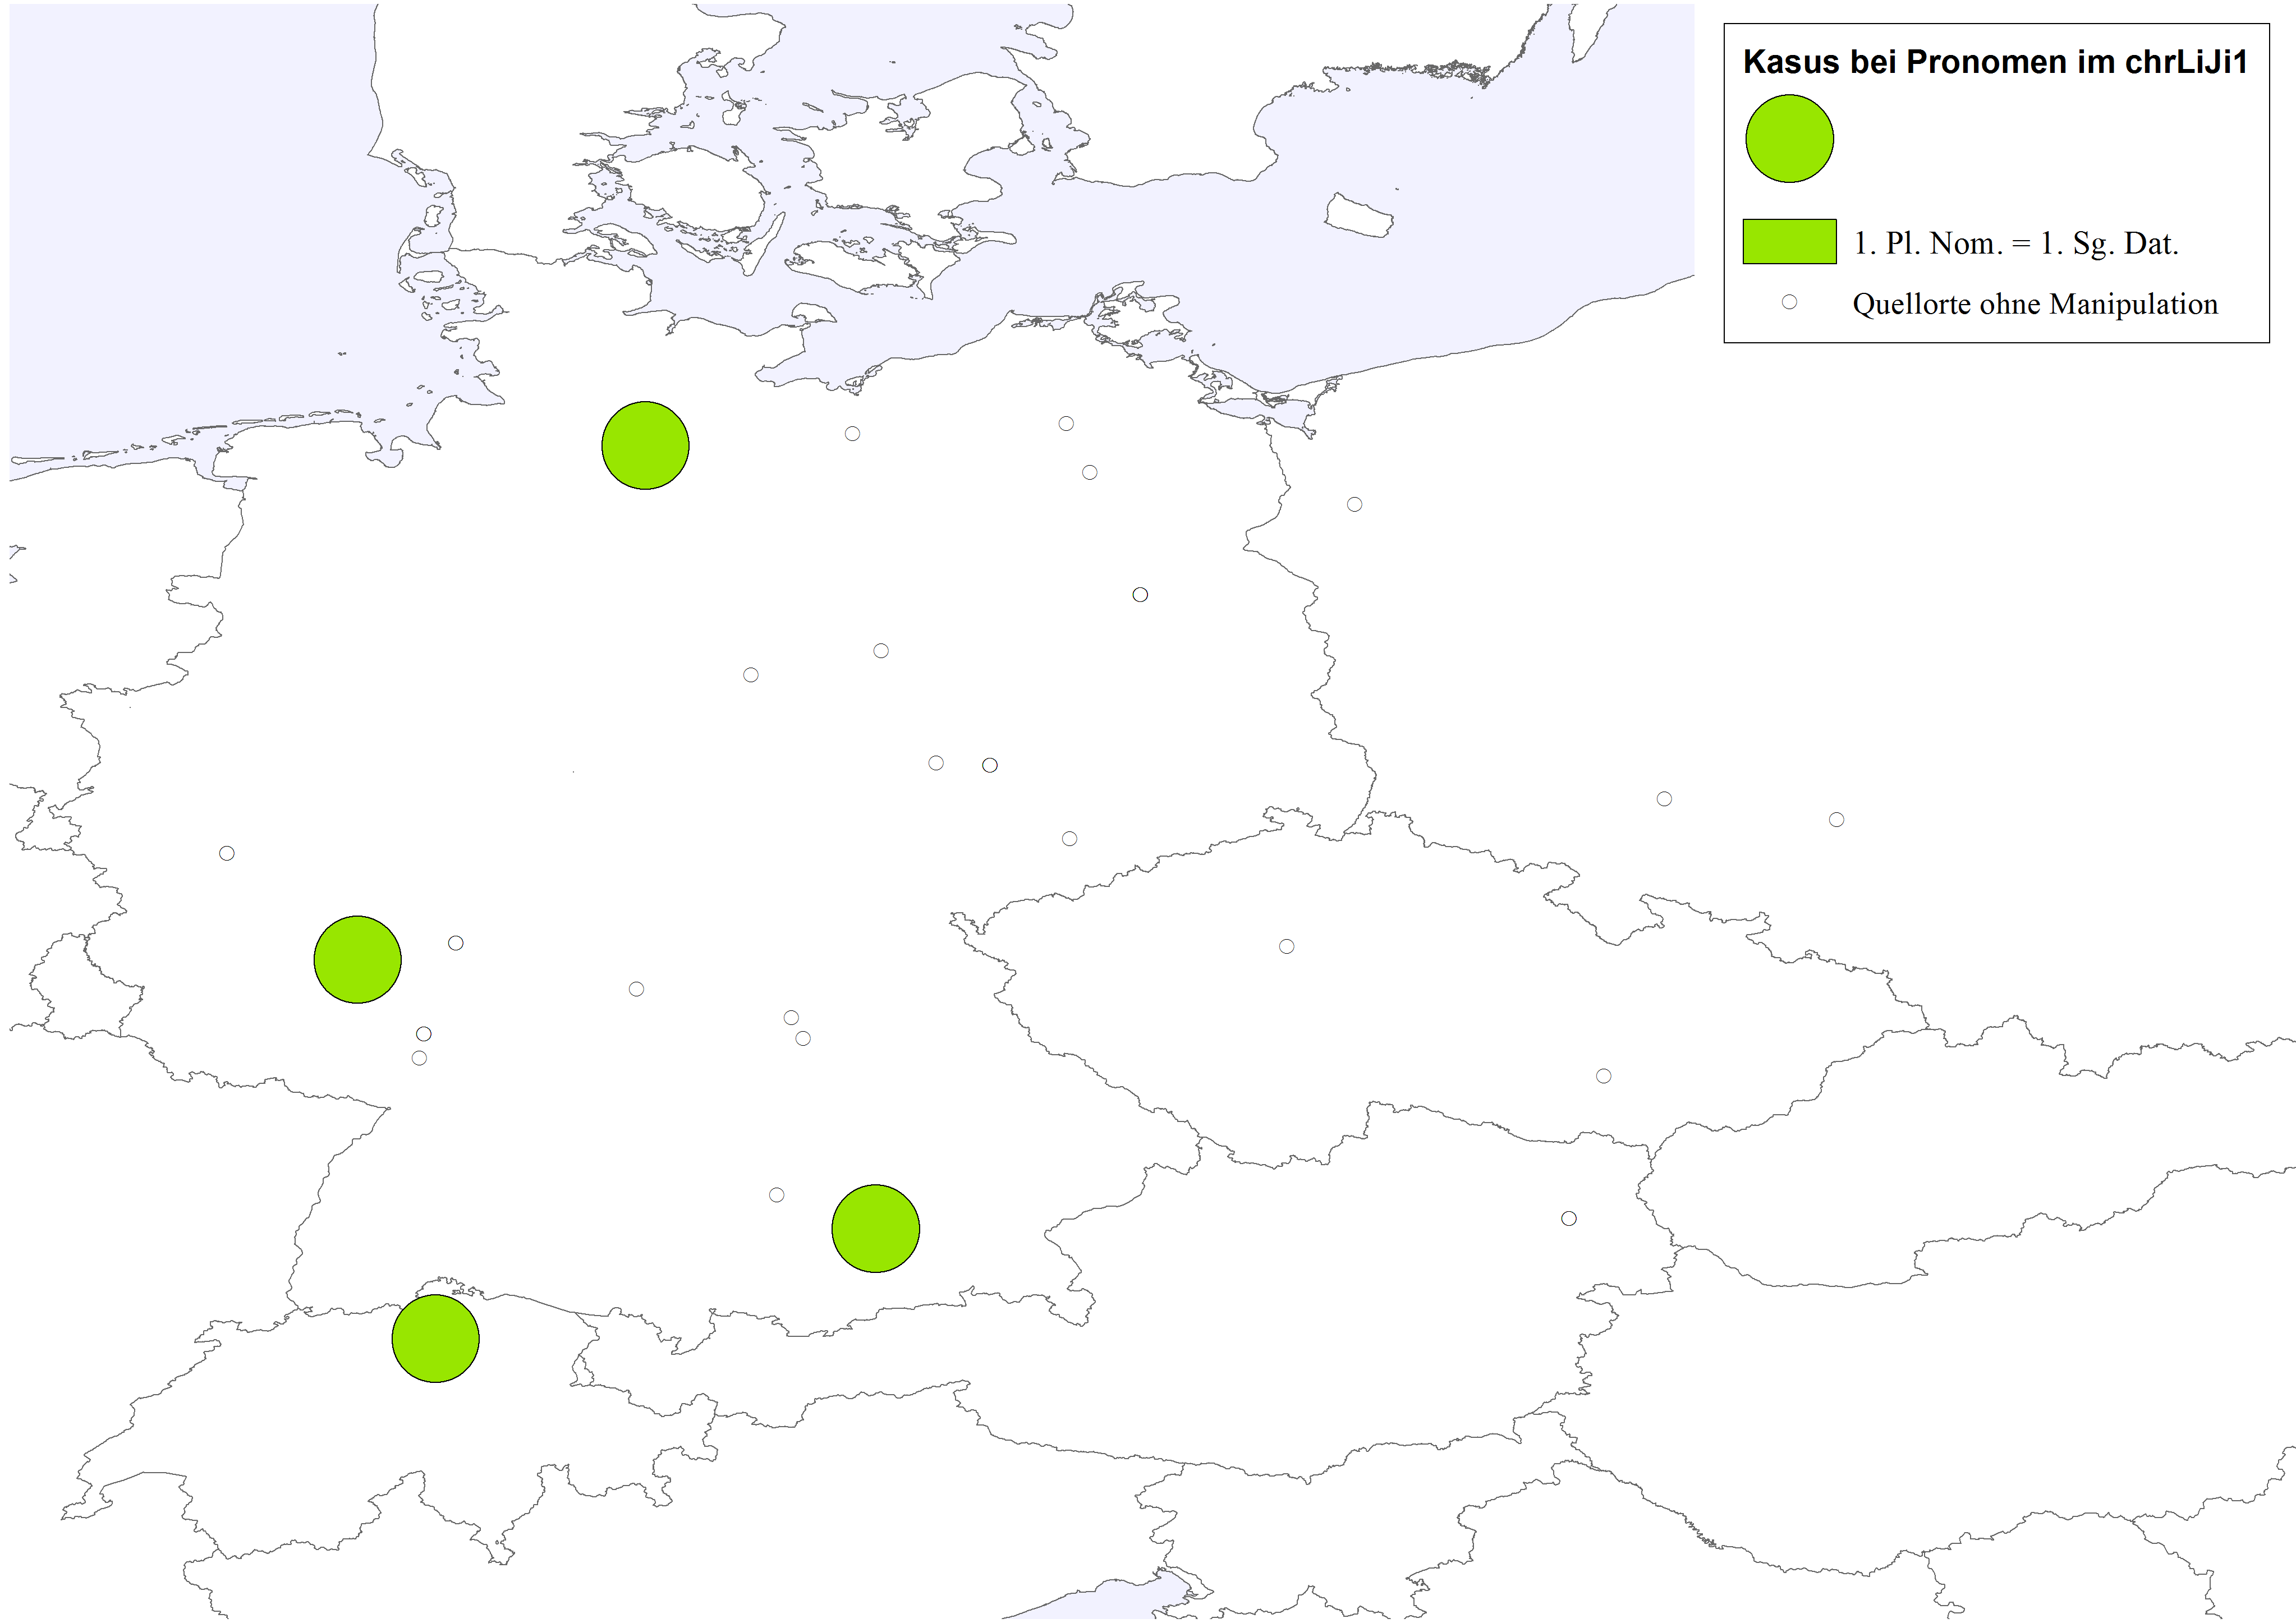
\includegraphics[height=.4\textheight]{figures/PRONOMEN_KARTE_1PLSYNKRETISMUS.png}
		\caption{\label{kartePRON4} \isi{Kasussynkretismus} der Personalpronomen 1. {\Pl} {\Nom} und 1. {\Sg} {\Dat} im \hai{chrLiJi1}}
		\end{figure}
  %farbe des meeres neu / heller!!!
	



\begin{figure}
\resizebox{\textwidth}{!}{
	\begin{tikzpicture}
		\begin{axis}[only marks, width=0.82\textwidth,height=0.32\textheight,
		legend style={at={(1,1)},xshift=+0.2cm, yshift=-0.15cm,anchor=north west,nodes=left},
			%title={Funktionstypen des sp\"aten Westjiddisch},
			xtick={1700, 1725, 1750, 1775, 1800, 1825, 1850, 1875, 1900, 1925, 1950, 1975}, ytick=\empty,
			x tick label style={/pgf/number format/1000 sep=}, 
			y tick label style={/pgf/number format/1000 sep=},
			%extra y ticks={456.1, 1022.4},
			%extra y tick labels={{456,1},{1022,4}},
			extra y tick style={grid=major,
				tick label style={, ,}},
				ymin=0.7,
				ymax=5.8,
			ylabel={Phänomenbelege},
			enlarge x limits=0.03]	

\addplot [mark=square, draw=black] table [x=jahr, y=1PLNOM_1SGDAT] {figures/Pronomen_1PLNOM_1SGDAT.txt};	
	
\addplot [ultra thick, mark=triangle*, gray] table [x=jahr, y=HOEF_NOM] {figures/Pronomen_HOEF_NOM.txt};			


\addplot [ultra thick, mark=triangle*, black] table [x=jahr, y=HOEF_DAT] {figures/Pronomen_HOEF_DAT.txt};
%


\addplot [mark=square*, gray] table [x=jahr, y=3SG_AKK] {figures/Pronomen_3SG_AKK.txt};	
	
\addplot [mark=square*, black] table [x=jahr, y=2SG_DAT] {figures/Pronomen_2SG_DAT.txt};			


\addplot [mark=*, gray] table [x=jahr, y=1SG_AKK] {figures/Pronomen_1SG_AKK.txt};


\addplot [mark=*, black] table [x=jahr, y=1SG_DAT] {figures/Pronomen_1SG_DAT.txt};



\addplot [mark=o,black] table [x=jahr, y=NO] {figures/Pronomen_NO.txt};%1.5
 

			% Andere Formen a={mark=square*,blue},% b={mark=triangle*,red},% c={mark=o,draw=black}}
						\legend{1. {\Pl} {\Nom} = 1. {\Sg} {\Dat}, Höfl. {\Nom}/{\Akk} statt {\Dat}, Höfl. {\Dat} statt {\Akk}, 3. {\Sg} {\mask} {\Akk} statt {\Dat} , 2. {\Sg} {\Dat} statt {\Akk}, 1. {\Sg} {\Akk} statt {\Dat}, 1. {\Sg} {\Dat} satt {\Akk}, keine Manipulation} %macht Legende
		\end{axis}
	\end{tikzpicture}
}
	\caption{Diachrone Verteilung von Synkretismen bei Personalpronomen im \hai{chrLiJi1}}
	\label{histokasusPRONOMEN}	
\end{figure}


Wie bereits beim Phänomen der Manipulationen am Kasus bei vollen Objekten nach \isi{Präposition} (vgl.\, Abbildung \ref{histokasusPP}) und in einfachen \hai{{\NP}}s (vgl.\, Abbildung \ref{histokasusNP}) zu sehen war, so zeigen auch die literaturjiddischen Eingriffe ins Pronominalsystem eine interessante Verteilung über die Zeitspanne hinweg (vgl.\, Abbildung \ref{histokasusPRONOMEN}). Auch dieses Phänomen gewinnt erst im Verlauf des 19. Jahrhunderts an Popularität innerhalb des \hai{chrLiJi1}.  Doch gibt es hier je nach \isi{Präposition} Unterschiede: So fällt ins Auge, dass die Setzung der Nominativ/Akkusativ-Form anstelle des Dativs in der Höflichkeitsform zwar noch im 18. Jahrhundert zu finden ist, aber im Laufe des 19. Jahrhunderts scheinbar \quein{abgelöst} wird durch das komplementäre Phänomen, der Setzung der Dativform anstelle des Akkusativs im Rahmen der Höflichkeitsform. Ähnliche Strukturen zeigt das \isi{Korpus} auch bei der Manipulation der Personalpronomen der 1. Person Singular: Die ältere und wesentlich seltener auftretende Manipulation ist die zugunsten des Akkusativs anstelle des Dativs. Ab 1825 nehmen aber Belege für die Setzung des Dativs anstelle des Akkusativs deutlich zu. Diachron ebenfalls auffällig verhält sich die Homophonie zwischen 1. Person Plural Nominativ mit der 1. Person Singular \isi{Dativ}. Dieses Phänomen, welches in den hochdeutschen Dialekten keine Seltenheit ist, findet sich im \hai{chrLiJi1} beinahe nur in Quellen aus dem letzten Drittel des 19. Jahrhunderts. 
	

		
Ein interessantes Raumbild liefert die Kartierung der Belege zur Manipulation der Höflichkeitspronomina (\ref{kartePRON3}). Mit der Ausnahme einer Frankfurter und einer Hamburger Quelle liegen alle übrigen Belege in nächster Nähe zum \hai{{\NÜJ}} bzw. \hai{{\SÜJ}}. Gegebenenfalls deuten die Daten des \hai{chrLiJi1} hier eine Eigenschaft dieser Varietäten an, die es durch authentischere Daten zu überprüfen gilt.
	
	 Interferenzen mit den deutschen Dialekten sind im Bereich der Pronomina durchaus anzunehmen. Zur Situation der pronominalen Anredeform in den deutschen Varietäten ist leider nichts flächendeckendes bekannt, womit die Daten des \hai{chrLiJi1} verglichen werden könnten. Die Belege für einen Akkusativ-Dativ-\isi{Synkretismus} in der 3. Person maskulin sprechen zwar für eine Anlehnung an das ostjiddische System, doch ist dies andererseits kein unüblicher \isi{Synkretismus} in den deutschen Dialekten. Nach \cite[426f]{Shrier1965} findet sich dieser etwa in großen Teilen des Niederdeutschen, Ostmitteldeutschen und Bairischen. Auch der \isi{Zusammenfall} von 1. Person Plural Nominativ unter die 1. Person Singular \isi{Dativ} ist ein in den hochdeutschen Mundarten weit verbreitetes Phänomen (vgl.\, \hai{WApron}:\,5). 
     Hier zeigt besonders die geographische Verteilung der Daten eine deutliche Überschneidung mit dem hochdeutschen Raum (s. Abbildung \ref{kartePRON4}).  Besonders aufschlussreich sind die Daten zur 1. Person Singular. Hier ist ein \isi{Synkretismus} von \isi{Akkusativ} und \isi{Dativ}, wie wir ihn im \hai{chrLiJi1} häufig antreffen, für die niederdeutschen Dialekte bekannt (\citealt[427f, 432 Karte 9]{Shrier1965}). Die Setzung des Akkusativs anstelle des Dativs ist hier besonders im Ostfälischen und Westbrandenburgischen verbreitet, während der \isi{Zusammenfall} zugunsten der Dativform im übrigen niederdeutschen Sprachgebiet auftritt. Ein großer Teil der Quellen, die diesen \isi{Synkretismus} zeigen, stammen aus dem niederdeutschen Raum und könnten so durch die deutschen Mundarten begünstigt sein (vgl.\, \ref{kartePRON2}). Bei allen Spekulationen über einen Einfluss der deutschen Dialekte darf nicht vergessen werden, dass nicht nur das \ili{Literaturjiddisch}, sondern  auch die tatsächlichen jiddischen Varietäten in ständigem \isi{Sprachkontakt} zu den deutschen Dialekten standen, aus dem Interferenzen hervorgegangen sind (vgl.\, \citealt{Schaefer2013}). Die Spuren deutscher Dialekte, die wir im \hai{{\LiJieins}} finden, schließen somit eine authentische Wiedergabe des jiddischen Sprachstandes nicht aus. Besonders aber die Belege einer Profilierung des Dativs gegenüber dem \isi{Akkusativ} im Singular sprächen für eine besondere Nähe des \hai{chrLiJi1} zum \hai{{\NÜJ}} und \hai{{\NOJ}} (s.\,o.).
     
     
     Die Daten des \hai{jüdLiJi1} unterstützen nur bedingt  diese Hypothese (Tabelle \ref{tblpronomenjüdLiJi1}). Hier findet sich fast ausschließlich eine starke Profilierung des Dativs gegenüber dem \isi{Akkusativ}, lediglich die Situation der Höflichkeitsform springt aus dem Rahmen. Besonders stark ist auch hier die 1. Person Singular von Manipulationen betroffen. Da ein Großteil der Quellen im Berliner Raum zu verorten ist, also einem Gebiet, in dem ebendieser \isi{Synkretismus} auch in den deutschen Dialekten stattfand  (vgl.\,  \citealt[427f, 432 Karte 9]{Shrier1965}), ist kaum zu entscheiden, ob eine Interferenz zwischen \ili{Literaturjiddisch} und deutschem Dialekt oder zwischen Jiddisch und deutschem Dialekt vorliegt.
     

	 
%      \todo{die folgenden abbildungen rutschen ins daruffolgende kapitel}
     
     


 
 
  \section{Verbmorphologie}\label{verbscheiße} 
 \subsection{Flexionen von \textit{sein}}\label{sein}
 %  %\noindent

 In zehn Quellen des \hai{chrLiJi1} finden sich Belege des unflektierten Infinitivs von \textit{sein} wie in (\ref{sein1})–(\ref{sein3}).  Das Suppletivverb \textit{sein}, dessen Paradigma aus mehreren Verbstämmen zusammengesetzt ist, zeigt in den meisten deutschen Dialekten Abweichungen von der Schriftsprache (\citealt[571–574]{Schirmunski1962}; \citealt{Nuebling2000}). Die Setzung des Infinitivs, wie es im \hai{chrLiJi1} vorliegt, ist jedoch nur für die \mbox{1. Person} Singular Präsens aus dem Oberhessischen bekannt (\citealt[572]{Schirmunski1962}; \citealt[93]{Friebertshaeuser1987}). Von diesen deutsch-dialektalen Formen scheint das Westjiddische jedoch nicht beeinflusst gewesen zu sein. So findet sich in \qu{Die Hochzeit zu Grobsdorf} im Sprechtext eines zentralhessisch redenden Bauers zwar die in diesem Dialektraum typische Form der 2. Person Singular Präsens \textit{seist} (\ref{seistgrobsdorf}, vgl.\, \citealt[93]{Friebertshaeuser1987}), jedoch im westjiddischen Haupttext taucht nirgends eine solche oberhessische Verbform auf, weder in der 2. Person Singular Präsens (\ref{bistgrobsdorf2}), noch in der 1. Person Singular Präsens (\ref{bingrobsdorf2}). Das Westjiddische in dieser Quelle entspricht bei der \isi{Flexion} von \textit{sein} immer der deutschen Schriftsprache. Das standardjiddische Paradigma von \RL{ז{יי}\makebox(-1.5,-3.5)[r]{\libertineGlyph{uni207B}}ן} \textit{seyn} unterscheidet sich im Präsens nur bezüglich der 1. und 3. Person Plural \RL{ז{{יי}\makebox(-1.5,-3.5)[r]{\libertineGlyph{uni207B}}}נען} \textit{saynen} (\hai{{\ZOJ}} \RL{זענען} \textit{senen}) \sem{sind} und der 2. Person Plural \RL{זענט} \textit{sent} \sem{seid} vom Schriftdeutschen (\citealt[216]{Jacobs2005}). Man könnte die Belege des \hai{chrLiJi1}, wo \textit{sein}/\textit{sain} in der 1., 2., 3. Person Singular Präsens und in der Höflichkeitsform auftritt (vgl.\, \ref{sein1}–\ref{sein3};Tabelle \ref{tblpronomenseinliji1}), \,%rs + Spatium
 mit einer Tilgung von \textit{-en} der ostjiddischen Form \textit{saynen} erklären. Eine solche Kürzung in der gesprochenen Sprache ist durchaus plausibel. Die \mbox{(zentral-)}ostjiddische Form der 1. und 3. Person Plural von \sem{sein} ist einzig in drei Quellen (\hai{AK} Zürich, 1948; \hai{DW} Wien, 1773 u. \hai{GW} n.a., ca.\, 1900) belegt (z.\,B.\, \ref{sennenAK}–\ref{sennenDW}). Da die Flexionslosigkeit also kaum auf einer \,%rs einer
 tatsächliche Sprechrealität fußen kann, ist anzunehmen, dass dieses Phänomen ausschließlich der Pejoration gilt. Erstmals hätten wir damit ein sprachliches Mittel, dessen sich das Literaturjiddische bedient, welches nicht auf einen möglichen Einfluss jiddischer oder deutscher Varietäten zurückgeführt werden kann.
 
\largerpage[2]

 \eenumsentence{
 \item \textit{bis ich sain ä raicher Jüd} \sem{bis ich ein reicher Jude bin} (\hai{JK} Breslau, 1810:\,5)\label{sein1}
 
 
  \item \textit{mer sein frei} \sem{wir sind frei} (\hai{LS} Bonn, 1925:\,26)\label{sein2}
 
 
 
  \item \textit{Die Kristche sein zwitschen sich selbst wahre Heidche!} \\
  \sem{Die Christen sind unter sich selbst wahre Heiden!} (\hai{WA}:\,158)\label{sein3b}


 
 \item \textit{Sie sein unser Retter} \sem{Sie sind unser Retter} (\hai{LS} Bonn, 1925:\,23)\label{sein3} 
 
 \item \textit{Mir alle sennen glicklich} \sem{Wir alle sind glücklich} (\hai{AK} Zürich, 1948:\,219)\label{sennenAK} 

 \item \textit{wenn alle a suy schlimm sennen} \sem{wenn alle so schlimm sind} (\hai{DW} Wien, 1773:\,16)\label{sennenDW} 



\item imitiertes hess. \RL{דא\makebox(-1.5,-7.5)[r]{\libertineGlyph{uni207B}}ן זייסט {ד{\makebox(0,9)[l]{\libertineGlyph{uni02D9}}{ו}}א} א\makebox(-1.5,-7.5)[r]{\libertineGlyph{uni207B}}הך א\makebox(-1.5,-7.5)[r]{\libertineGlyph{uni207B}}הן {א\makebox(-1.25,-1.25)[r]{\libertineGlyph{uni05B8}}}רמער שעלם} \\
\textit{dan seist dou ahch ahn oremer schelm}\\
 \sem{dann bist (wörtl. seist) du auch ein armer Schelm}\\
(\qu{Die Hochzeit zu Grobsdorf} 1822:\,2)\label{seistgrobsdorf}


\item {\wj} \RL{ד{א\makebox(-1.25,-1.25)[r]{\libertineGlyph{uni05B8}}}ס דוא פון גר{א\makebox(-1.25,-1.25)[r]{\libertineGlyph{uni05B8}}}בסדארף ביסט}\\
 \textit{dos du fun grobsdorf bist} \\
 \sem{dass du aus Grobsdorf bist}\\  
 (\qu{Die Hochzeit zu Grobsdorf} 1822:\,9)\label{bistgrobsdorf2}

\largerpage
\item {\wj} \RL{איך בין {א\makebox(-1.25,-1.25)[r]{\libertineGlyph{uni05B8}}}בער אה קערלכה}\\
 \textit{ich bin ober ah kerlche} \\
 \sem{Ich bin aber ein Kerlchen}\\
 (\qu{Die Hochzeit zu Grobsdorf} 1822:\,8)\label{bingrobsdorf2}

 }
 
 \begin{table}
%\begin{longtable}{ccc|ccc}
 \begin{center}
		\begin{tabular}{lllll}
		\lsptoprule 

\textbf{Quelle} &\textbf{1. {\Sg}}  & \textbf{1. {\Pl}} &  \textbf{3. {\Pl}}  &\textbf{Höflichkeitsform}\\ \midrule 


\hai{LS} &  \textit{sein}  & \textit{sein} &– &  \textit{sein} \\
\hai{JK} &  \textit{sain}  & \textit{sain}/ \textit{sayn}   && \\
\hai{MS} & – & –& \textit{sein} & –\\
\hai{DP} & – & – &  \textit{sain}  &  \textit{sain}  \\
\hai{PAb} & –  & –&–& \textit{sain}  \\
\hai{WA} & –&– & \textit{sein} &– \\
\hai{FM} &– & \textit{sein}  &–&– \\
\hai{JP} & –& \textit{sein}  & \textit{sein} &– \\
\hai{LP} & –&– &\textit{sein} &\textit{sein}  \\
\hai{GW} &– &– &–&\textit{sein}  \\
	
  \lspbottomrule 

 \end{tabular}\end{center}
		 \caption{Unflektiertes \sem{sein} im \hai{chrLiJi1}}
		 \label{tblpronomenseinliji1}
		 \end{table}
		% \end{longtable}	

 
Die areale Verteilung der Belege für unflektiertes \textit{sein} im \hai{chrLiJi1} zeigt deutlich eine Anhäufung im \hai{{\NÜJ}} und \hai{{\SÜJ}} (Abbildung \ref{kartesein}). Aber auch im mitteldeutschen Raum (Bonn, Frankfurt), wo immerhin in den oberhessischen Dialekten diese Form für die 1. Person Singular bekannt ist, findet sich dieses Phänomen. Belege für die zentralostjiddische Form \textit{sennen} findet sich ausschließlich in südlichen Quellen.

\begin{figure} 

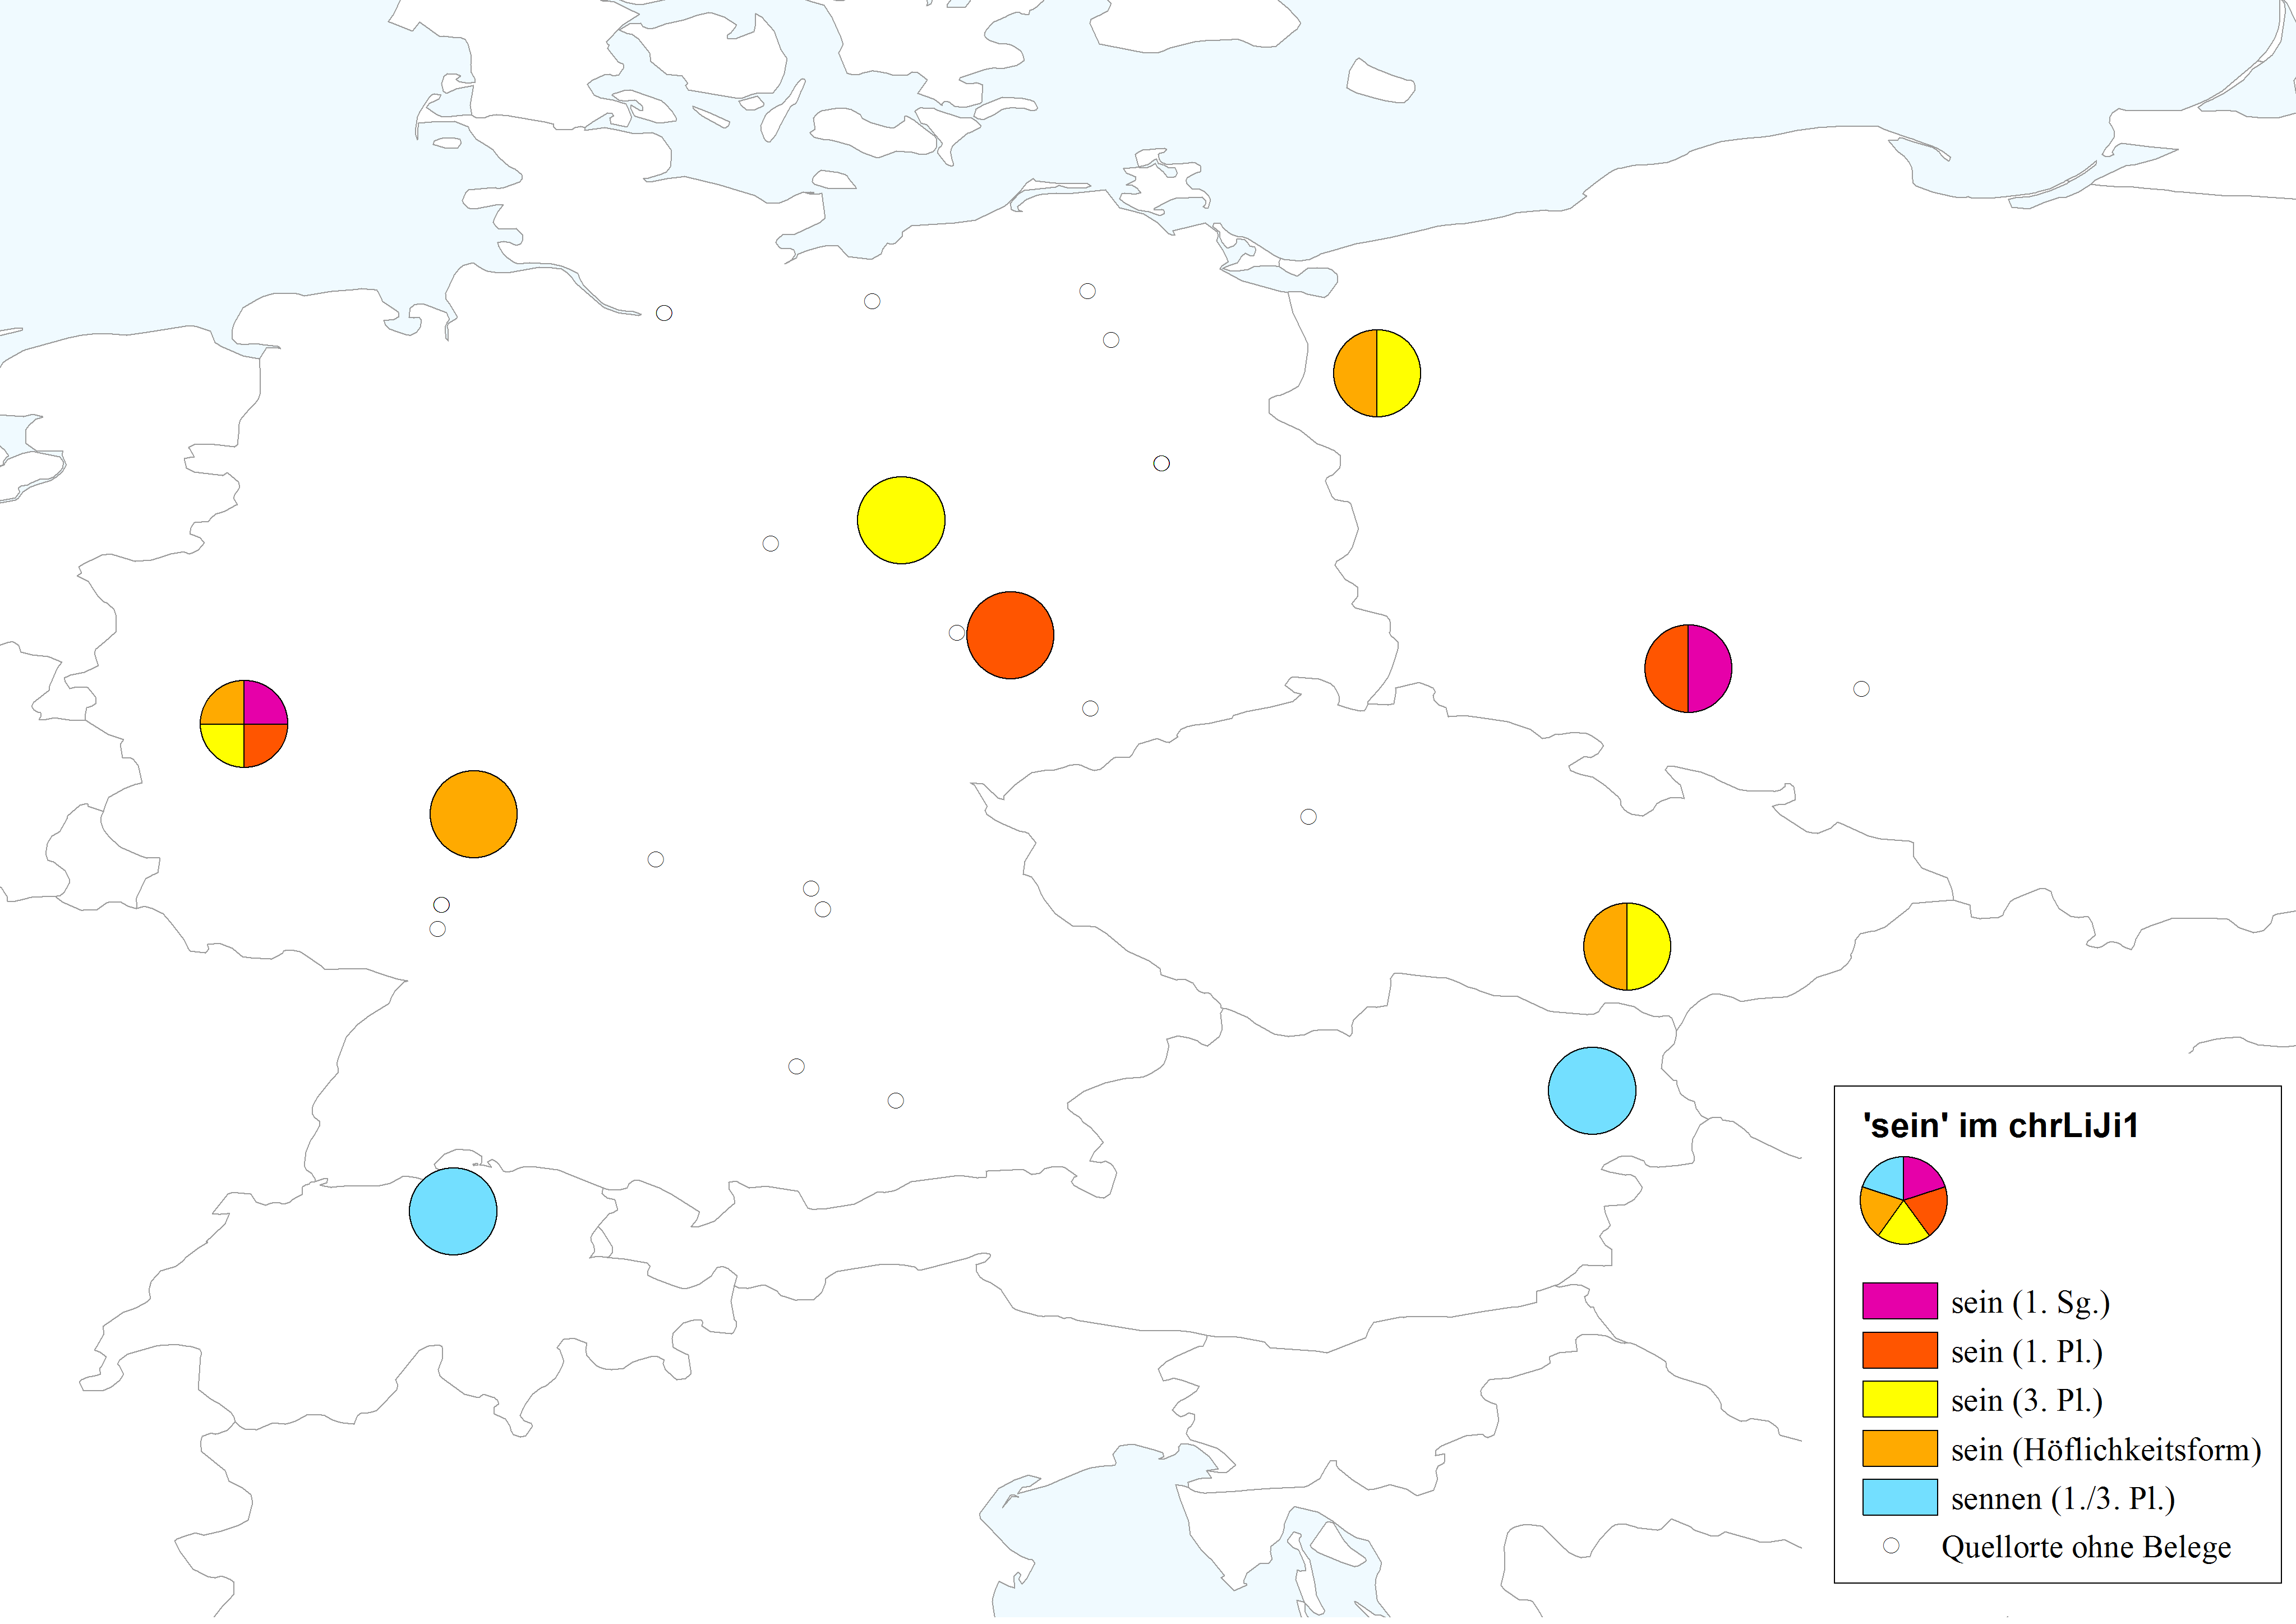
\includegraphics[width=\textwidth]{figures/sein.png}
		\caption{\label{kartesein} Flexionen  von \sem{sein} im \hai{chrLiJi1}}
		\end{figure}
  


Besonders auffällig gestaltet sich die zeitliche Streuung des Phänomens (s. Abbildung \ref{histosein}). \,%rs + "s. Abbildung" 
Obzwar zentral\ili{ostjiddisch} \textit{sennen} schon in den frühesten Quellen belegt ist, treten Belege für unflektiertes \textit{sein} erst im 19. Jahrhundert – insbesondere in der 2. Hälfte des Jahrhunderts – auf. Auch hier zeigt das \hai{{\LiJieins}} eine morphologische Manipulation erstmals in den späteren Quellen.

%\todo{Changed Legend Style, inserted a resizebox} 
\begin{figure} 
\resizebox{\textwidth}{!}{\begin{tikzpicture}
		\begin{axis}[only marks, width=0.82\textwidth,height=0.24\textheight,
			legend style={legend pos=outer north east, cells={anchor=west},font=\footnotesize},
% 		        legend style={at={(1,1)},xshift=+0.2cm, yshift=-0.1cm,anchor=north west,nodes=left},
			%title={Funktionstypen des sp\"aten Westjiddisch},
			xtick={1700, 1725, 1750, 1775, 1800, 1825, 1850, 1875, 1900, 1925, 1950, 1975}, ytick=\empty,
			x tick label style={/pgf/number format/1000 sep=}, 
			y tick label style={/pgf/number format/1000 sep=},
			%extra y ticks={456.1, 1022.4},
			%extra y tick labels={{456,1},{1022,4}},
			extra y tick style={grid=major,
				tick label style={, ,}},
				ymin=0.1,
				ymax=4.5,
			ylabel={Phänomenbelege},
			enlarge x limits=0.03]	
                \addplot [mark=*, gray] table [x=jahr, y=SENNEN] {figures/sein_SENNEN.txt};	
                \addplot [mark=square*, gray] table [x=jahr, y=HOEF] {figures/sein_HOEF.txt};	
                \addplot [mark=square*, black] table [x=jahr, y=3PL] {figures/sein_3PL.txt};		
                \addplot [ultra thick, mark=triangle*, black] table [x=jahr, y=1PL] {figures/sein_1PL.txt};
                \addplot [mark=*, black] table [x=jahr, y=1SG] {figures/sein_1SG.txt};
                \addplot [mark=o,black] table [x=jahr, y=NO] {figures/sein_NO.txt};%1
 		% Andere Formen a={mark=square*,blue},% b={mark=triangle*,red},% c={mark=o,draw=black}}
		\legend{\textit{sennen} (1./3. {\Pl}), \textit{sein} (Höfl.), \textit{sein} (3. {\Pl}), \textit{sein} (1. {\Pl}), \textit{sein} (1. {\Sg}),  keine Manipulation} %macht Legende
		\end{axis}
	\end{tikzpicture}}
	\caption{Diachrone Verteilung der Flexionen  von \sem{sein} im \hai{chrLiJi1}}
	\label{histosein}	
\end{figure}


Es überrascht, dass sich unflektiertes \sem{sein} auch im \hai{jüdLiJi1} findet (Tabelle \ref{tblpronomenseinjuedliji1}). 
Zentralostjiddisches \textit{sennen} in der Position der 1. und 3. Person Plural Präsens findet sich in den \qu{Gedichten und Scherzen in jüdischer Mundart} (\hai{GuS1}, \hai{GuS5}, \hai{GuS10}, \hai{GuS23}). Die unflektierte Form tritt im \hai{jüdLiJi1}, wie im \hai{chrLiJi1}, in der 1. Person Singular/Plural, der 3. Person Plural sowie (in einem Beleg)\footnote{Hinter der Form \textit{seun} (\hai{GuS1}:\,5) könnte sich jedoch auch ein Konjunktiv verbergen.} in der Höflichkeitsform auf (vgl.\, Tabelle \ref{tblpronomenseinjuedliji1}). Die Belege im \hai{jüdLiJi1} entsprechen auch der Verbreitung im \hai{chrLiJi1} (vgl.\, Abbildung \ref{kartesein}).


Es muss offen bleiben, wie dieses Phänomen zu interpretieren ist; ob nun als \quein{fehlerhafte Flexion}, die eine \quein{Fehlerhaftigkeit der Sprache} darstellen soll, oder sich dahinter eine Kürzung von \ili{Ostjiddisch} \textit{saynen} verbirgt, die im tatsächlich gesprochenen Jiddisch gegeben war. Für das Eindringen einer ostjiddischen Form spricht die diachrone Streuung: Erst ab Mitte des 19. Jahrhundert kann man von einem Bewusstsein der ostjiddischen Sprache in der gesellschaftlichen Breite ausgehen. Hingegen ist auch gerade das späte Auftreten dieses Phänomens im \hai{{\LiJieins}} ein Indiz für eine \quein{fiktive} Form, da ab etwa 1850 der direkte \isi{Sprachkontakt} zum gesprochenen (West-)Jiddischen nur mehr äußerst gering ausfällt.


\begin{table} 
  \begin{tabular}{lllll}
  \lsptoprule 

  \textbf{Quelle} &\textbf{1. {\Sg}}  & \textbf{1. {\Pl}} &  \textbf{3. {\Pl}}  &\textbf{Höflichkeitsform}\\ \midrule 



  \hai{GuS1} &– &– &–&\textit{seun}  \\
  \hai{PBerlin1} &– &\textit{sein} &\textit{sein}&–  \\
  \hai{PBerlin2} &\textit{sein} &\textit{sein} &\textit{sein}&–  \\


\lspbottomrule
  \end{tabular} 
  \caption{Unflektiertes \sem{sein} im \hai{jüdLiJi1}}
  \label{tblpronomenseinjuedliji1}
\end{table} 

\subsection{{\textit{ge}-Präfix} bei sekundärem Wortakzent}\label{ge}
%  %\noindent	
\ref{GEYES}
In den modernen Standardsystemen des Jiddischen und Deutschen können nur erstbetonte Verbstämme ihr \isi{Partizip} mittels des \textit{ge-}Präfix bilden 
(\ref{GEYESji}) und (\ref{GEYES}).
Mehrfüßige und damit nicht erstbetonte Partizipien, wie in 
(\ref{GENOji}) und (\ref{GENO}), %\,%rs + und
 können kein Präfix hinzuziehen (\citealt[213]{Jacobs2005}; \citealt[92]{Wiese2000}). Dies betrifft besonders Fremdwörter 
 (\ref{GENO}). 
 Bei Partikelverben wird im Jiddischen wie im Deutschen das {\textit{ge}}-Präfix gesetzt, da hier die \isi{Partikel} einen eigenen \isi{Wortakzent} trägt z.\,B.\, (\ref{GEPartikel1dt}), (\ref{GEPartikel1oj}). Bei Präfixverben wie in (\ref{GEPartikel1}) und (\ref{GEPartikel1q}) hingegen entfällt das Präfix aufgrund des Wortakzents (vgl.\, \citealt[213]{Jacobs2005}; \citealt[92]{Wiese2000}). Allerdings liegen prosodische Unterschiede zwischen Jiddisch und Deutsch vor, so dass ein Verb  wie \textit{übersetzen} in (\ref{GEPartikel1})–(\ref{GEPartikel1q}) im Deutschen den \isi{Wortakzent} eines Präfixverbs zeigt, im Jiddischen hingegen \textit{über-} als \isi{Partikel} intoniert wird und dementsprechend mittels \textit{ge-}Präfix flektiert wird (\ref{uebersetzen1OJ}). Da uns im \hai{{\LiJi}} nur schriftsprachliches Material vorliegt, ist es akustisch nicht zu entscheiden, ob ein Präfix oder eine \isi{Partikel} vorliegt. Daher sind Belege aus periphrastischen Verben nur unter Vorbehalt zu beurteilen.

\eenumsentence{
	\item {\oj} {\RL{שר{יי}\makebox(-1.5,-3.5)[r]{\libertineGlyph{uni207B}}בן}} \textit{shraybn} $\to$  {\RL{געשריבן}} \textit{geschrieben}/ {\RL{שריבן*}} \textit{schrieben}\label{GEYESji}
	\item \textit{schreiben $\to$  geschrieben/*schrieben}\label{GEYES}

\item {\oj} {\RL{שטודירן}} \textit{shtudirn} $\to$  {\RL{געשטודירט*}} \textit{geshtudirt}/ {\RL{שטודירט}} \textit{studirt}\label{GENOji}
\item dt. \textit{studieren $\to$ *gestudiert/studiert}\label{GENO}

	\item dt. \textit{\textipa{\textprimstress}an\textipa{\textsecstress}schreiben} $\to$ \textit{angeschrieben}/*\textit{anschrieben}\label{GEPartikel1dt} %Partikelverb1Dt

\item {\oj} {\RL{אנשר{{יי}\makebox(-1.5,-3.5)[r]{\libertineGlyph{uni207B}}}בן}} \textipa{\textprimstress}\textit{on}\textipa{\textsecstress}\textit{shraybn}  $\to$ {\RL{אנגעשריבן}}\textit{ongeshribn}/ {\RL{אנשריבן*}} \textit{onshribn}\label{GEPartikel1oj} %Partikelverb1\ili{OJ}
	
	\item dt. \textit{\textipa{\textprimstress}über\textipa{\textsecstress}setzen} $\to$ \textit{übergesetzt}/*\textit{übersetzt};z.\,B.\, \textit{Er ist mit dem Boot übergesetzt.}\label{GEPartikel1} %Partikelverb

\item dt. \textit{\textipa{\textsecstress}über\textipa{\textprimstress}setzen} $\to$ *\textit{übergesetzt}/\textit{übersetzt};z.\,B.\, \textit{Er hat das Buch übersetzt.}\label{GEPartikel1q}%Präfixverb


\item {\oj} {\RL{ז{{יי}\makebox(-1.5,-3.5)[r]{\libertineGlyph{uni207B}}}נע ביכער […] ז{{יי}\makebox(-1.5,-3.5)[r]{\libertineGlyph{uni207B}}}נען געוו{א\makebox(-1.25,-1.25)[r]{\libertineGlyph{uni05B8}}}רן איבערגעזעצט אויף א\makebox(-1.5,-7.5)[r]{\libertineGlyph{uni207B}}נדערע ש{פ\makebox(-1,4)[r]{\libertineGlyph{afii57807}}}רא\makebox(-1.5,-7.5)[r]{\libertineGlyph{uni207B}}כן}} \\
\textit{zayne bikher} […] \textit{zaynen gevorn ibergesetst oyf andere shprakhn}\\
\sem{Seine Bücher […] wurden in andere Sprachen übersetzt}.
(zitiert n. \hai{CMY} 
{\RL{לעבנס־{{פ\makebox(-0.8,9)[r]{\libertineGlyph{uni207B}}}}רא\makebox(-1.5,-7.5)[r]{\libertineGlyph{uni207B}}גן}}
 2007.09-10)\label{uebersetzen1OJ}
}

Der Blick auf eine andere germanische Sprache mit \textit{ge}-\isi{Partizip}, das Niederländische, zeigt, dass die Regel der Erstbetonung keine Grundeigenschaft dieses Suffixes ist. So entsprechen im modernen Niederländischen Formen wie (\ref{GEYESNDL}) \,%rs sonst keine Klammern
 durchaus dem Standard (\citealt{Rathert2009}). Und auch in älteren Sprachstufen des Deutschen (\ref{GEYESMHD}), (\ref{GEYESFRNH}) und in einigen deutschen Dialekten (\ref{GEYESHOHENEMS}) wirkt diese Regel nicht. So verwundert es kaum, dass auch für das Westjiddische Formen belegt sind, in denen das Präfix trotz sekundärem \isi{Wortakzent} auftritt (\ref{BspGEGROBS}).


\eenumsentence{
%	\item dt. \textit{besprechen $\to$ *gebesprochen/besprochen}\label{GENOPRAE}	
	\item  {\ndl} \textit{studeren $\to$ gestudeert/*studeert} (zitiert n. \citealt[164]{Rathert2009})\label{GEYESNDL}
	\item {\aleman} \textit{marschiera $\to$ g’marschiert} (Hohenems (AT), zitiert n. \citealt[255]{Schallert2012})\label{GEYESHOHENEMS}
	\item  {\mhd} \textit{studieren $\to$  gestudiert} (zitiert n. Rathert 2009:\,164)\label{GEYESMHD}
	\item {\frnhd} \textit{er habe denn zuvor durch ander leute hulff gestudiret} \\(M. Luther, zitiert n. \hai{DWB} \citealt[Bd. 20, Sp. 275]{DeutschesWB})\label{GEYESFRNH}
  
  \item {\wj} {\RL{איץ ווא\makebox(-1.5,-7.5)[r]{\libertineGlyph{uni207B}}רד אופפעם דא\makebox(-1.5,-7.5)[r]{\libertineGlyph{uni207B}}נץ געמא\makebox(-1.5,-7.5)[r]{\libertineGlyph{uni207B}}רשירט}} \\
  \textit{iz ward uffem danz gemarschirt} \\
  \sem{Jetzt wird auf den Tanz marschiert.}\\
  (\qu{Die Hochzeit zu Grobsdorf} 1822:\,53) \label{BspGEGROBS}
   
 }

Im \hai{chrLiJi1} finden sich einige wenige Belege für die Setzung des \textit{ge-}Präfix bei sekundärem \isi{Wortakzent} in fünf Quellen (\ref{ge1}–\ref{ge5}). Im Fall von \ref{ge4} \,%rs () streichen
liegt uns zwar ein Verstoß gegen den deutschen \isi{Wortakzent} vor, allerdings entspricht dieser Beleg der ostjiddischen Form, in der \textit{über}- als \isi{Partikel} und nicht als Präfix getrennt wird (\ref{uebersetzen1OJ}). Es fällt auf, dass im \hai{{\LiJi}} besonders Fremdwörter mit mehrsilbigem \,%rs -m
Präfix das \textit{ge-}Präfix aufweisen.  Auch sind nicht nur Partikelverben betroffen, sondern auch Fremdwörter, die im Deutschen auf Grund des Wortakzents im \isi{Partizip} das \textit{ge-}Präfix nicht zu sich nehmen (vgl.\, \ref{ge2q}–\ref{ge1q}).  Zeitlich tritt dieses Phänomen besonders in der Frühphase des \hai{{\LiJi}} auf. Besonders im Vergleich zu unseren Daten aus dem \hai{{\ZWJ}} (\ref{BspGEGROBS}) wiegt der Umstand, dass wir diese Quellen des \hai{chrLiJi1} neben Berlin besonders auf den mitteldeutschen sprich zentralwestjiddischen Raum verorten. \,%rs wir…verorten
Wieder kann damit nicht ausgeschlossen werden, dass hier entweder deutsch-dialektale Formen, oder aber authentisch westjiddische Strukturen ins \hai{chrLiJi1} Eingang gefunden haben. 
	%Ein Beleg zeigt dieses Phänomen auch bei Nominalisierung (\ref{geNOMINALISIERUNG}).
	
		 \eenumsentence{

  \item \textit{ausgemöbliert} \sem{ausmöbliert} (\hai{LM} Würzburg, 1844:\,Titel)\label{ge1}
  
 \item \textit{ausgestudiert} \sem{ausstudiert} (\hai{LM} Würzburg, 1844:\,Titel)\label{ge2}
 
 \item \textit{gestudiert} \sem{studiert} (\hai{FE} Leipzig, 1792:\,71)\label{ge2b}

 
 \item \textit{übergelassen} \sem{überlassen} (\hai{AJ} Berlin, 1825:\,2), vgl.\, {\oj} \RL{איבערגעל{א\makebox(-1.25,-1.25)[r]{\libertineGlyph{uni05B8}}}זן} \textit{ibergelozn} \label{ge4}%\ili{OJ}

 \item \textit{geprofitiert} \sem{profitiert} (\hai{AJ} Berlin, 1825:\,1)\label{ge2q}
 
\item \textit{gepaßirt} \sem{passiert} (\hai{FL} Mannheim, 1778:\,39)\label{ge1q}

  \item \textit{gespezziren} \sem{spazieren} (\hai{MV} Berlin, 1862:\,60)\label{ge5}

}


Für ein mögliches Areal sprechen auch Belege aus dem \hai{jüdLiJi1}, wo, besonders in den \qu{Gedichten und Scherzen in jüdischer Mundart}, aber auch in den Berliner Pamphleten, die {\textit{ge}}-Präfigierung an nicht-erstsilbenbetonten Verben zu finden sind (\ref{ge6})--(\ref{ge12}). 

 \eenumsentence{
 \item \textit{geamüserirt} \sem{amüsiert} (\hai{GuS1}:\,4, 5)\label{ge6}


 \item \textit{getransportirt} \sem{transportiert} (\hai{GuS5}:\,3)\label{ge7}


 \item \textit{geexpedirt }\sem{expediert} (\hai{GuS5}:\,4)\label{ge8}


 \item \textit{getaxirt} \sem{taxiert} (\hai{GuS5}:\,4)\label{ge9}


 \item \textit{eingequartiert} \sem{einquartiert} (\hai{GuS15}:\,4)\label{ge10}


 \item \textit{gepassirt} \sem{passiert} (\hai{PBerlin1}:\,2)\label{ge11}

 
 \item \textit{gepessirt/gepassiert} \sem{passiert} (\hai{PBerlin2}:\,1.Sp., 2.Sp.)\label{ge12}

 	} 
    
      \section{Zusammenschau morphologischer Manipulationen}\label{fazitmorph}
%\noindent
In der Summe finden sich 19 morphologische Phänomene, die wiederholt in den Quellen des \hai{chrLiJi1} eingesetzt werden. Darunter finden sich vorwiegend Verletzungen des Standarddeutschen Kasussystems. Das heißt auch, dass vorwiegend die Nominalmorphologie beeinflusst wird. Die Verbalmorphologie wird nur mit zwei Strategien (\textit{sein} \sem{bin} u. \textit{ge}-\isi{Partizip}) manipuliert. Das häufigste Phänomen ist die Setzung des Akkusativs an der Position von Schriftdeutsch \isi{Dativ} im Singular (in 17 Quellen gegeben). Am seltensten treten Manipulationen am Kasus voller Objekte auf. Im Durchschnitt zeigt eine Quelle 2,4 morphologische Manipulationsstrategien ({$\sigma$}\,2,1). Die Quelle mit der höchsten Phänomendichte morphologischer Manipulationen ist \hai{PA} (Frankfurt, 1834) mit sieben Phänomenen, gefolgt von \hai{AD} (Leipzig, 1846), \hai{AJ} (Berlin, 1825), \hai{JP} (Altona, 1867) und \hai{SV} (München, 1890) mit je sechs Phänomenen.

Wie das Diagramm in Abbildung \ref{allstreumorph} \,%rs Abbildung 
 zeigt, treten morphologische Manipulationen im gesamten Untersuchungszeitraum auf. In den Quellen des Intervalls 1825 bis 1875 lässt sich ein vergleichsweise höheres Aufkommen morphologischer Strategien erkennen.

%streudiagramm morphologie %HILFE!!!! Ab lich-Dim Farben um eins verschoben!!!?!?!?!?! %TT
 
 \begin{figure} 
 \farbgrafik
	\begin{tikzpicture}
		\begin{axis}[only marks, width=0.82\textwidth,height=0.40\textheight,
		legend style={at={(1,1)},xshift=+0.2cm, yshift=-0cm,anchor=north west,nodes=left, font=\tiny},
			%title={Funktionstypen des sp\"aten Westjiddisch},
			xtick={1700, 1725, 1750, 1775, 1800, 1825, 1850, 1875, 1900, 1925, 1950, 1975}, ytick=\empty,
			x tick label style={/pgf/number format/1000 sep=}, 
			y tick label style={/pgf/number format/1000 sep=},
			%extra y ticks={456.1, 1022.4},
			%extra y tick labels={{456,1},{1022,4}},
			extra y tick style={grid=major,
				tick label style={, ,}},
				ymin=24.1,
				ymax=43.9,
				y=3.45mm,
			ylabel={Phänomene},
			enlarge x limits=0.03]	

%\isi{Morphologie}	
		
\addplot [very thick, mark=triangle*,  BrickRed] table [x=jahr, y=sein] {figures/all_sein_43.txt};
\addplot [very thick, mark=triangle*, WildStrawberry] table [x=jahr, y=Pluralsuffix] {figures/all_Pluralsuffix_42.txt};
\addplot [very thick, mark=triangle*, teal] table [x=jahr, y=PronomenHOEF_DAT] {figures/all_PronomenHOEF_DAT_41.txt};
\addplot [very thick, mark=triangle*, black] table [x=jahr, y=PronomenHOEF_NOM] {figures/all_PronomenHOEF_NOM_40.txt};
\addplot [very thick, mark=triangle*, green] table [x=jahr, y=Pronomen1PLNOM_1SGDAT] {figures/all_Pronomen1PLNOM_1SGDAT_39.txt};
\addplot [very thick, mark=triangle*, gray] table [x=jahr, y=Pronomen3SG_AKK] {figures/all_Pronomen3SG_AKK_38.txt};
 \addplot [very thick, mark=triangle*, Thistle] table [x=jahr, y=Pronomen2SG_DAT] {figures/all_Pronomen2SG_DAT_37.txt};
\addplot [very thick, mark=triangle*, Melon] table [x=jahr, y=Pronomen1SG_AKK] {figures/all_Pronomen1SG_AKK_36.txt};
\addplot [very thick, mark=triangle*, CornflowerBlue] table [x=jahr, y=Pronomen1SG_DAT] {figures/all_Pronomen35SG_DAT_35.txt};
\addplot [very thick, mark=triangle*, magenta] table [x=jahr, y=KasusPraepPL_DAT] {figures/all_KasusPraepPL_DAT_34.txt};
\addplot [very thick, mark=triangle*, ForestGreen] table [x=jahr, y=KasusPraepPL_AKK
] {figures/all_KasusPraepPL_AKK_33.txt};
\addplot [very thick, mark=triangle*, Dandelion] table [x=jahr, y=KasusPraepDAT_statt_AKK
] {figures/all_PraepDAT_statt_AKK_32.txt};
\addplot [very thick, mark=triangle*, SkyBlue] table [x=jahr, y=KasusPraepAKK_statt_DAT] {figures/all_PraepAKK_statt_DAT_31.txt};
 \addplot [very thick, mark=triangle*, YellowGreen] table [x=jahr, y=KasusnvolleNPPL_NOM] {figures/all_KasusnvolleNPPL_NOM_30.txt};
  \addplot [very thick, mark=triangle*, RoyalPurple] table [x=jahr, y=KasusnvolleNPSG_M_DAT] {figures/all_KasusnvolleNPSG_M_DAT_29.txt};
\addplot [very thick, mark=triangle*, orange] table [x=jahr, y=KasusnvolleNPSG_M_NOM] {figures/all_KasusnvolleNPSG_M_NOM_28.txt};
\addplot [very thick, mark=triangle*, Maroon] table [x=jahr, y=OJ_GENUS] {figures/all_OJGenus_27.txt};
\addplot [very thick, mark=triangle*, Goldenrod] table [x=jahr, y=gePartizip] {figures/all_gePart_26.txt};
\addplot [very thick, mark=triangle*, LimeGreen] table [x=jahr, y=lichPL] {figures/all_lichPL_25.txt};


\legend{\textit{sein}, Pluralsuffixe, {\Pron} Höfl.{\Dat}, {\Pron} Höfl.{\Nom}, {\Pron} 1.{\Pl}{\Nom}=1.{\Sg}{\Dat}, {\Pron} 3.{\Sg}Akk, {\Pron} 2.{\Sg}Dat, {\Pron} 1.{\Sg}Akk, {\Pron} 1.{\Sg}{\Dat}, Kasus (\hai{{\PP}}) {\Pl}{\Dat},  Kasus (\hai{{\PP}}) {\Pl}{\Akk}, Kasus (\hai{{\PP}}) {\Sg}{\Dat}, Kasus (\hai{{\PP}}) {\Sg}{\Akk}, Kasus (\hai{{\NP}}) {\Pl}{\Nom}, Kasus (\hai{{\NP}}) {\Pl}{\mask}{\Dat}, Kasus (\hai{{\NP}}) {\Sg}{\mask}{\Dat}, Kasus (\hai{{\NP}}) {\Sg}{\mask}{\Nom}, {\oj} \isi{Genus}, \textit{ge-}\isi{Partizip}, \textit{-lich} {\Pl} {\Dim}} %macht Legende
		\end{axis}
	\end{tikzpicture}
	\caption{Übersicht morphologischer Markierungen im \hai{chrLiJi1}}
	\label{allstreumorph}	
\end{figure}
%  \todo{Hier wäre es sehr schön, wenn Legende und Diagramm in Linie wären}


Die areale Distribution morphologischer Phänomene, gewichtet nach Distanz-basierter Interpolation (\hai{IDW}), zeigt ein durchaus interessantes Bild. Wie in Karte \ref{karteIDWMORPH} zu sehen, treten in Quellen aus dem  Westen des Untersuchungsgebiets deutlich mehr morphologische Markierungen auf. Der Südwesten zeigt damit ähnlich, wie dies bereits bezüglich der phonologischen Phänomene der Fall war (vgl.\, Abbildung \ref{kartelijiIDWQGIS}, \ref{kartelijiIDW}, S.\, \ref{kartelijiIDWQGIS}), eine deutliche höhere Phänomenvielfalt als andere Regionen. Dennoch unterscheidet sich die Verteilung morphologischer Phänomene von der phonologischer deutlich. 

\begin{figure} 

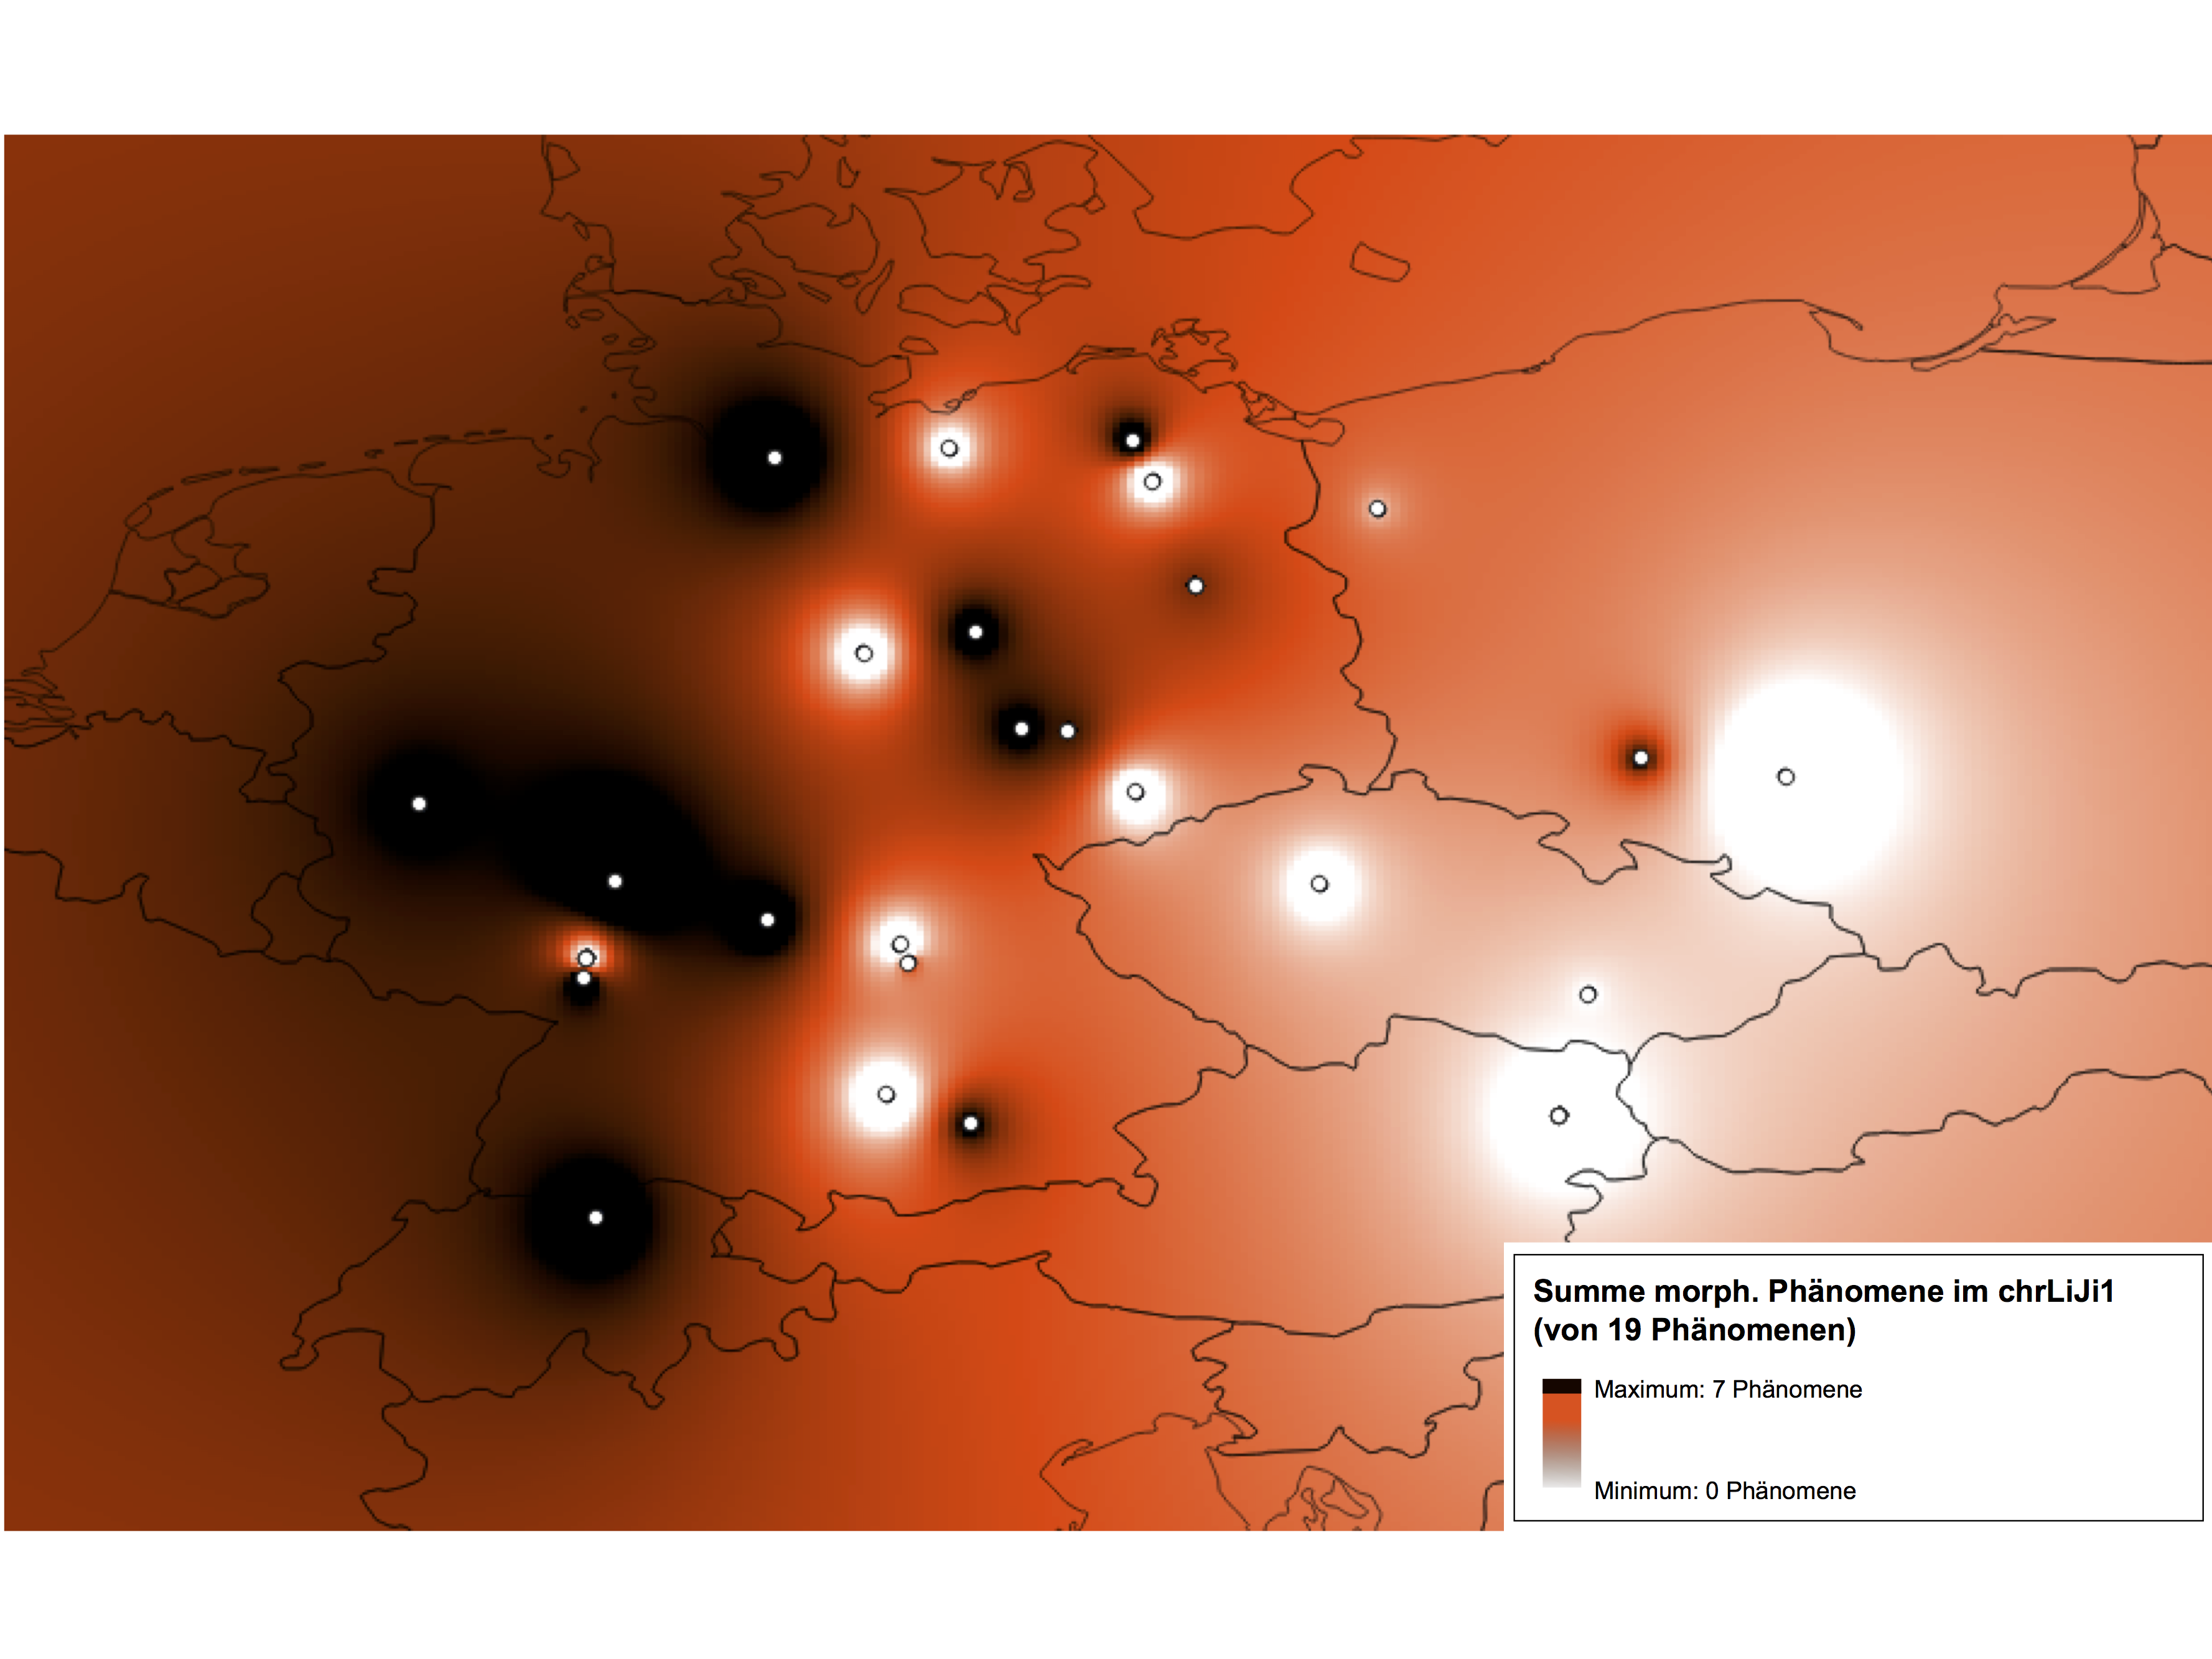
\includegraphics[width=\textwidth]{figures/morph_IDW_legende.png}
		\caption{\label{karteIDWMORPH} Summe morphologischer Phänomene des \hai{chrLiJi1} (\hai{IDW} berechnet mit \hai{QGIS})}
		\end{figure}
  

In der \isi{Morphologie} sind die quantitativen Schwankungen zwischen der Verwendung von vielen und gar keinen Phänomenen besonders gravierend: entweder erfüllt eine Quelle nahezu alle der 19 Phänomene oder aber gar keine, im Gegensatz zur Phonologie (vgl.\, Kapitel \ref{fazitphon}, S.\, \pageref{fazitphon}), wo eine \quein{Zwischenzone} zu erkennen ist (vgl.\, Abbildung \ref{kartelijiIDW}, S.\, \ref{kartelijiIDW}). 